\chapter{Web 2.0}\label{ch:ch2}

\subsubsection{2.1.1}

According to a number of scholars, the rise of Twitter publishing had to lead a new level of informational openness in social networks and to increase of press freedom. At the same time, some recent studies have shown significant criticism towards political efficacy of Twitter [7] (нужен источник). We analyze Twitter as a part of the hybridized media system [6] (нужен источник) suggesting after Adam and Pfetsch [1] (нужен источник) that political dimension of hybridization and spill-over effects between different media will be specific to the socio-political context. In terms of the media system modernization [15] (нужен источник) and hybridization context, Russian media system is the one bearing both unique and post-Communist-specific features. In our research, we aim at analyzing the role of Twitter in the process of agenda setting in the hybridized media system in Russia and finding out if the use of Twitter potentially leads to the formation of the ‘crossroads of opinions' or, in contrast, to encapsulation of political discussion and further fragmentation of public discourse.Our research focuses on structural and content aspects of discussion on anti-migrant bashings in Biryulyovo (Moscow) in October 2013. Methods of research include automated web crawling, framing analysis via semantic coding, and interpretation of descriptive statistics. Preliminary results suggest unexpectedly high level of mediatization of the discussion. The ‘crossroads' nature of the discussion showed up but in such a way that makes Twitter differ from elite communicative milieus like the Russian Facebook.

\subsubsection{2.4.1}

The community-based structure of communication on social networking sites has long been a focus of scholarly attention. However, the problem of discovery and description of hidden communities, including defining the proper level of user aggregation, remains an important problem not yet resolved. Studies of online communities have clear social implications, as they allow for assessment of preference-based user grouping and the detection of socially hazardous groups. The aim of this study is to comparatively assess the algorithms that effectively analyze large user networks and extract hidden user communities from them. The results we have obtained show the most suitable algorithms for Twitter datasets of different volumes (dozen thousands, hundred thousands, and millions of tweets). We show that the Infomap and Leiden algorithms provide for the best results overall, and we advise testing a combination of these algorithms for detecting discursive communities based on user traits or views. We also show that the generalized K-means algorithm does not apply to big datasets, while a range of other algorithms tend to prioritize the detection of just one big community instead of many that would mirror the reality better. For isolating overlapping communities, the GANXiS algorithm should be used, while OSLOM is not advised. 

\subsubsection{2.4.2}

Despite disputable possibility of extension of analysis of social relations on Twitter to real life, Twitter discussions are still being under attention of scholars studying structures and meanings of news- and issue-based ad-hoc public discourse. One of the socially relevant aspects of Twitter studies is that of influencers -- accounts that produce impact, either inside or outside Twitter. But there is still no agreement in the research community on how to defme and measure who is an influencer: either by 'absolute figures' or by network analysis metrics; this issue is even rarely discussed. Politically, today's mediatized public sphere where traditional media play the role of information hubs is highly uneven in terms of access to opinion expression; it privileges institutional players, including political elites, corporations, and media themselves. Hopes that Twitter would provide a more equal space for public deliberation are still not proven enough. Using web crawling and manual assessment of Twitter ad-hoc discussion on the Biryulyovo bashings of 2013, we show that users who post or even get commented most do not make it to the positions of most 'central' users by network metrics. We also demonstrate that usen that rank high by betweenness and pagerank centntrality form circles of reciprocal commenting that show the social cleavage wider than the discussion itself.

\subsubsection{2.4.3}

Today, a range of research approaches is used to define the so-called influencers in discussions in social media, and one can trace both conceptual and methodological differences in how influencers are defined and tracked. We distinguish between ‘marketing’ and ‘deliberative’ conceptualization of influencers and between metrics based on absolute figures and those from social network analytics; combining them leads to better understanding of user activity and connectivity measures in defining influential users. We add to the existing research by asking whether user activity necessarily leads to better connectivity and by what metrics in online ad hoc discussions, and try to compare the structure of influencers. To do this, we use comparable outbursts of discussions on inter-ethnic conflicts related to immigration. We collect Twitter data on violent conflicts between host and re-settled groups in Russia and Germany and look at top20 user lists by eight parameters of activity and connectivity to assess the structure of influencers in terms of pro/contra-migrant cleavages and institutional belonging. Our results show that, in both discussions, the number of users involved matters most for becoming an influencer by betweenness and pagerank centralities. Also, contrary to expectations, Russian top users all in all are, in general, more neutral, while Germans are more divided, but in both countries pro-migrant media oppose anti-migrant informal leaders.

\subsubsection{2.4.4}

Abstractive summarization is a technique that allows for extracting condensed meanings from long texts, with a variety of potential practical applications. Nonetheless, today’s abstractive summarization research is limited to testing the models on various types of data, which brings only marginal improvements and does not lead to massive practical employment of the method. In particular, abstractive summarization is not used for social media research, where it would be very useful for opinion and topic mining due to the complications that social media data create for other methods of textual analysis. Of all social media, Reddit is most frequently used for testing new neural models of text summarization on large-scale datasets in English, without further testing on real-world smaller-size data in various languages or from various other platforms. Moreover, for social media, summarizing pools of texts (one-author posts, comment threads, discussion cascades, etc.) may bring crucial results relevant for social studies, which have not yet been tested. However, the existing methods of abstractive summarization are not fine-tuned for social media data and have next-to-never been applied to data from platforms beyond Reddit, nor for comments or non-English user texts. We address these research gaps by fine-tuning the newest Transformer-based neural network models LongFormer and T5 and testing them against BART, and on real-world data from Reddit, with improvements of up to 2\%. Then, we apply the best model (fine-tuned T5) to pools of comments from Reddit and assess the similarity of post and comment summarizations. Further, to overcome the 500-token limitation of T5 for analyzing social media pools that are usually bigger, we apply LongFormer Large and T5 Large to pools of tweets from a large-scale discussion on the Charlie Hebdo massacre in three languages and prove that pool summarizations may be used for detecting micro-shifts in agendas of networked discussions. Our results show, however, that additional learning is definitely needed for German and French, as the results for these languages are non-satisfactory, and more fine-tuning is needed even in English for Twitter data. Thus, we show that a ‘one-for-all’ neural-network summarization model is still impossible to reach, while fine-tuning for platform affordances works well. We also show that fine-tuned T5 works best for small-scale social media data, but LongFormer is helpful for larger-scale pool summarizations.

\subsubsection{2.4.5}

\textit{Objectives.} Social media have become a place where the bulk of grassroots political discussion takes place. Today, the growing body of research is dedicated to cumulative patterns on online deliberation, the predecessors of which were the concept of the spiral of silence, the silent majority hypothesis, and influencer studies. However, when applied to the dissonant, disruptive, and discontinued online discussions of today where gatewatching is much less predictable and cumulation of support is often accompanied by communicative aggression, these concepts need to be reconsidered and re-tested. Also, the current public communication online is much more multi-level than before; even within one platform, several communication layers may be defined, and their inter-relations in terms of public opinion aggregation remain under-studied. \textit{Research goal.} This paper aims at discovering patterns of cumulative deliberation in online communication. We first discuss the umbrella concept of cumulative deliberation. Then, we test the dynamics of the discussion on Belarusian oppositional YouTube in terms of impact of cross-account commenting on growth of commenting within the cross-account community and the overall discussion. \textit{Method and sampling.} We have collected the data by YouTube crawling. The data include all user comments of 2018 for six salient Belarusian oppositional accounts. To define the cross-account commenters, we used Gephi-based web graph reconstruction. We manually coded user posts for interactivity, aggression, and criticism. Dependencies in the dynamics of the discussion were tested by correlational and cluster analysis. \textit{Results.} We have discovered that users diverged into two mutually exclusive modes of expression, namely aggressive-dialogical and (self-)critical. Of the cross-account commenters, several users demonstrated ‘cumulative’ behavior and personal opinion bubbles. While there were nearly no dependencies discovered in the dynamics of user posting, criticism and self-criticism show capacity of spurring/diminishing the dynamics of public communication online, even if commenting on the whole is cumulative, not dialogical.

\subsubsection{2.4.6}

Agendas in online media have become a scholarly focus nearly two decades ago, leading to shifting conceptualizations of what we see as agenda. Thus, agendas and agenda shifts \textit{inside} online discussions have shown its potential to influence offline deliberation, aggregate support, fuel protest, passing through and/or bypassing traditional media’s gatekeeping. Real-time (or nearly-real-time) learning about quick agenda movement inside globalized public debate might be particularly important for international organizations like UN or EU. However, we today lack both knowledge on how agendas move in such discussions and instruments on such analysis. In particular, we are next-to-unaware of to what extent globally relevant themes get contextualized within language-based discussion segments, as well as to what extent the latter depend on each other and lag behind each other in developing agendas and public opinion on quickly evolving issues or conflicts. In this paper, we propose a method of agenda detection based on neural-network text summarization and compare summaries of tweet packages across three languages within the Twitter hashtag \#jesuischarlie. We show that sentiment detection may allow for quality assessment of the text summaries, as compared to aggregated sentiment to the original tweets. We show that, outside France, agendas were more interpretational, abstract, and non-contextualized. The pattern of news changing to ‘issue outburt’ was simultaneous in dense discussion segments and lagged behind in a sparser one. We also show that, globally, main issues of the discussion may be spotted within the first hour.

\subsubsection{2.4.7}

With the emergence of discussion platforms like Twitter, the hopes rose that computermediated public sphere would become more even in access to discussion than massmediatized public sphere of the late 20th century. Scholars have argued that it will eventually form an ‘opinion crossroads’ where conflicts would be discussed by all the parties involved. But today, existing research provides mixed evidence on whether ordinary users, rather than mainstream media and institutional actors, can become influencers in discussions on current issues, e.g. relations between host and migrant communities. We focus on the Twitter discussion about an inter-ethnic conflict in Moscow’s Biryuliovo district in 2013, as well as the comparative ‘calm’ period in March 2014, and look at who were real influencers by reconstructing the discussion’s web graph, as well as analyzing and juxtaposing its metrics to figures indicating user activity. Our results show that ad hoc discussion differs dramatically from an issuebased one in terms of the influencer nature and composition; the role of active tweeting is questioned. We also show that nationalist accounts play a much bigger role than expected in both periods.

\subsubsection{2.5.1}

Конфликты с участием переселенцев «с глобального Юга» и их обсуждение в медиа и социальных сетях стали чертой современной публичной сферы в Европе и России. Сетевые дискуссии способны играть роль групп давления в формировании повестки обсуждения миграции и принятия политических решений, актуализируя как конфликтные, так и консенсусные общественные настроения. Важно знать, существуют ли закономерности в том, кого пользователи сети (в том числе иститутциональные) видят как виновников конфликтов и от кого ожидают его разрешения. Мы рассматриваем четыре конфликтные дискуссии в Твиттере в России и Германии 2013--2016 гг. и оцениваем связь статуса пользователя с паттернами присвоения вины и ответственности, а также сопоставляем дискурсивные стратегии обвинения в двух странах. Методология исследования включает веб-краулинг по заданному словарю, экспертную оценку аккаунтов пользователей, ручное кодирование твитов и описательную статистику. Итоги исследований говорят о том, что в целом обвинение направлено в первую очередь против трех групп: региональных властей, нацилнального лидера/правительства и иммигрантов; разрешения конфликтов пользователи ждут от федеральных властей, ответственных за изменение иммиграционной политики. Но если в Германии очевиден политический разлом между правыми (пронационалистическими) и левыми (феминистскими) стратегиями поиска виноватых, то в российском Твиттере доминирует обвинение и власти, и иммигрантов, а также распространены сниженные ожидания мирной политической разрядки межэтнической напряженности.

\subsubsection{2.5.2}

Recently, the growing role of social network users in content dissemination has brought to life the concept of secondary gatekeeping -- selection and republication of content already selected and published by traditional gatekeepers. Secondary gatekeeping is believed to be raising the media in-platform visibility, but it may also have negative effects such as adding to creation of echo chambers and deepening the gaps between conflicting views. Such studies are particularly relevant for emergencies or social conflicts where sharing relevant content may be crucial for lowering social unease. But till today the nature of secondary gatekeeping remains highly understudied. We have conducted a comparative study of three \textit{ad-hoc} Twitter discussions on heated ethnic/racial conflicts in the USA (Ferguson riots), Germany (Köln mass abuse), and Russia (Biryulyovo anti-migrant bashings) to assess the patterns of content sharing by active discussants. We used vocabulary-based web crawling and human coding of over 1,000 tweets in randomized samples. Our results show that, in all cases, there’s weak but significant correlation between the type of user and his/her attitude to minority with the attitudes expressed in content, while it is not always true that users prefer the same gatekeeper type, e.g. online or social media. As difference between individual users remains statistically significant, this may mean that the nature of heated \textit{ad-hoc} discussions facilitates formation of ‘individual-level filter bubbles’ in addition to bigger echo chambers.

\subsubsection{2.5.3}

With growth of Internet communication, hopes rose that online discussions will equalize ordinary users and institutional discussants. But what roles traditional media play in online discussions remains under-researched. We argue that mediatization of Twitter discourse is worth studying, as activity of registered media in online discussions may play a role in preserving the “offline” deliberative inequalities. To assess the roles of media in Twitter discussions, we look at two structural aspects of their presence: posting activity and users’ sharing of media content -- within heated \textit{ad hoc} Twitter discussions on inter-ethnic conflicts in Russia, the USA, and Germany. Our findings show huge national differences in mediatization patterns, including the roles of political media. But also we see that, in all the three cases, the discourse is shaped by “white majority media”, and outlets that would represent the oppressed minority are virtually absent in both posting and link sharing patterns.

\subsubsection{2.5.4}

Online communication platforms have rapidly become a substantial element of e-governance processes in Europe and beyond. Today, research has shown that, in cases of social unrest and/or emergency, political actors responsible for their resolution are able to efficiently use microblogging platforms (including Twitter) to promote the discourse of harmonization. But in today's Russia, where the growth of inter-ethnic conflicts between the re-settlers from the post-Soviet South (Central Asia and South Caucasus) and the host communities in cities and towns has coincided with the growth of online communication milieus and their radicalization, political actors as well as NGOs seem to play minor roles in online communication management, including the cases of social unrest. We explore two Twitter discussions on inter-ethnic conflicts in Moscow to describe the presence of political actors, their roles in conflict resolution, and the patterns of expectations of other users towards the politicians. We discover extremely low political participation, as well as the phenomenon of 'radical replacement' of the roles of political emergency managers by nationalist users.

\subsubsection{2.5.5}

Embeddedness of politicians and political organizations in a discussion defines its level of institutionalization and creates a public arena for collaboration between publics and institutional actors. Thus, testing whether traditional hierarchies (in terms of presence of politically institutionalized actors) show up in online discussions deserves scholarly research. Moreover, it is also important to see whether more democratic societies show patterns of public involvement of politically institutionalized users that would differ from those in more authoritarian contexts.

To assess the ‘influencer’ status of politically institutionalized actors on Twitter cross-culturally, we have selected conflictual Twitter discussions in Germany, the USA, and Russia, all based on violent inter-ethnic clashes. Using vocabulary-based web crawling, we collected data on them and formed samples of top users selected by four activity metrics and five network metrics, to assess the positions of political users in the top lists and correlations of user status with their top list ranks. To this, we added qualitative assessment of presence of political users in comparative perspective.

Our results show that, in all the cases, presence of political actors in online discussions is scarce; also, political actors tend to fail to link user groups or stay in the center of discussion. There is also meaningful divergence of Russia from the pattern that Germany and the USA show: while in these countries politicians gain user attention based on content, in Russia it is the status itself that matters, and political users tend to gain weight in the discussion structure despite low attention levels.

\subsubsection{2.5.6}

YouTube-based discussions are a growing area of academic attention. However, we still lack knowledge on whether YouTube provides for forming critical publics in countries with no established democratic tradition. To address this question, we study commenting to Belarusian oppositional YouTube blogs in advance of the major wave of Belarusian post-election protests of 2020. Based on the crawled data of the whole year of 2018 for six Belarusian political videoblogs, we define the structure of the commenters’ community, detect the core commenters, and assess their discourse for aggression, orientation of dialogue, direction of criticism, and antagonism/agonism. We show that, on Belarusian YouTube, the commenters represented a genuine adversarial self-critical public with cumulative patterns of solidarity formation and find markers of readiness for the protest spillover.

\section{Концептуальное назначение}\label{sec:ch2/sec1}

%\begin{figure}[ht]
%    \centerfloat{
%        \includegraphics[scale=0.27]{latex}
%    }
%    \caption{TeX.}\label{fig:latex}
%\end{figure}
%
%Для выравнивания изображения по-центру используется команда \verb+\centerfloat+, которая является во
%многом улучшенной версией встроенной команды \verb+\centering+.

\section{Принципы построения ресурсов}\label{sec:ch2/sect2}

%А это две картинки под общим номером и названием:
%\begin{figure}[ht]
%    \begin{minipage}[b][][b]{0.49\linewidth}\centering
%        \includegraphics[width=0.5\linewidth]{knuth1} \\ а)
%    \end{minipage}
%    \hfill
%    \begin{minipage}[b][][b]{0.49\linewidth}\centering
%        \includegraphics[width=0.5\linewidth]{knuth2} \\ б)
%    \end{minipage}
%    \caption{Очень длинная подпись к изображению,
%        на котором представлены две фотографии Дональда Кнута}
%    \label{fig:knuth}
%\end{figure}
%
%Те~же~две картинки под~общим номером и~названием,
%но с автоматизированной нумерацией подрисунков:
%\begin{figure}[ht]
%    \centerfloat{
%        \hfill
%        \subcaptionbox[List-of-Figures entry]{Первый подрисунок\label{fig:knuth_2-1}}{%
%            \includegraphics[width=0.25\linewidth]{knuth1}}
%        \hfill
%        \subcaptionbox{\label{fig:knuth_2-2}}{%
%            \includegraphics[width=0.25\linewidth]{knuth2}}
%        \hfill
%        \subcaptionbox{Третий подрисунок, подпись к которому
%            не~помещается на~одной строке}{%
%            \includegraphics[width=0.3\linewidth]{example-image-c}}
%        \hfill
%    }
%    \legend{Подрисуночный текст, описывающий обозначения, например. Согласно
%        ГОСТ 2.105, пункт 4.3.1, располагается перед наименованием рисунка.}
%    \caption[Этот текст попадает в названия рисунков в списке рисунков]{Очень
%        длинная подпись к второму изображению, на~котором представлены две
%        фотографии Дональда Кнута}\label{fig:knuth_2}
%\end{figure}
%
%На рисунке~\cref{fig:knuth_2-1} показан Дональд Кнут без головного убора.
%На рисунке~\cref{fig:knuth_2}\subcaptionref*{fig:knuth_2-2}
%показан Дональд Кнут в головном уборе.
%
%Возможно вставлять векторные картинки, рассчитываемые \LaTeX\ <<на~лету>>
%с~их~предварительной компиляцией. Надписи в таких рисунках будут выполнены
%тем же~шрифтом, который указан для документа в целом.
%На~рисунке~\cref{fig:tikz_example} на~странице~\pageref{fig:tikz_example}
%представлен пример схемы, рассчитываемой пакетом \verb|tikz| <<на~лету>>.
%Для ускорения компиляции, подобные рисунки могут быть <<кешированы>>, что
%определяется настройками в~\verb|common/setup.tex|.
%Причём имя предкомпилированного
%файла и~папка расположения таких файлов могут быть отдельно заданы,
%что удобно, если не~для подготовки диссертации,
%то~для подготовки научных публикаций.
%\begin{figure}[ht]
%    \centerfloat{
%        \ifdefmacro{\tikzsetnextfilename}{\tikzsetnextfilename{tikz_example_compiled}}{}% присваиваемое предкомпилированному pdf имя файла (не обязательно)
%        %\input{Dissertation/images/tikz_scheme.tikz}
%
%    }
%    \legend{}
%    \caption[Пример \texttt{tikz} схемы]{Пример рисунка, рассчитываемого
%        \texttt{tikz}, который может быть предкомпилирован}\label{fig:tikz_example}
%\end{figure}
%
%Множество программ имеют либо встроенную возможность экспортировать векторную
%графику кодом \verb|tikz|, либо соответствующий пакет расширения.
%Например, в GeoGebra есть встроенный экспорт,
%для Inkscape есть пакет svg2tikz,
%для Python есть пакет tikzplotlib,
%для R есть пакет tikzdevice.

\section{Сбор данных}\label{sec:ch2/sec3}

%\noindent Нумерованный список:
%\begin{enumerate}
%    \item Первый пункт.
%    \item Второй пункт.
%    \item Третий пункт.
%\end{enumerate}
%
%\noindent Маркированный список:
%\begin{itemize}
%    \item Первый пункт.
%    \item Второй пункт.
%    \item Третий пункт.
%\end{itemize}
%
%\noindent Вложенные списки:
%\begin{itemize}
%    \item Имеется маркированный список.
%          \begin{enumerate}
%              \item В нём лежит нумерованный список,
%              \item в котором
%                    \begin{itemize}
%                        \item лежит ещё один маркированный список.
%                    \end{itemize}
%          \end{enumerate}
%\end{itemize}
%
%\noindent Нумерованные вложенные списки:
%\begin{enumerate}
%    \item Первый пункт.
%    \item Второй пункт.
%    \item Вообще, по ГОСТ 2.105 первый уровень нумерации
%          (при необходимости ссылки в тексте документа на одно из перечислений)
%          идёт буквами русского или латинского алфавитов,
%          а второй "--- цифрами со~скобками.
%          Здесь отходим от ГОСТ.
%          \begin{enumerate}
%              \item в нём лежит нумерованный список,
%              \item в котором
%                    \begin{enumerate}
%                        \item ещё один нумерованный список,
%                        \item третий уровень нумерации не нормирован ГОСТ 2.105;
%                        \item обращаем внимание на строчность букв,
%                        \item в этом списке
%                              \begin{itemize}
%                                  \item лежит ещё один маркированный список.
%                              \end{itemize}
%                    \end{enumerate}
%
%          \end{enumerate}
%
%    \item Четвёртый пункт.
%\end{enumerate}

\section{Анализ пользовательских Web-графов}\label{sec:ch2/sec4}

\subsection{Detection of Hidden Communities in Twitter Discussions of Varying Volumes}\label{subsec:ch2/sec4/sub1}

\subsubsection{1. Introduction}

With the growth of the Internet, its complexity has also grown substantially. In particular, social networking has provided for formation of user clusters corresponding to an increasingly big number of communities at various levels, up to the cross-platform one. As previous research states, the formation of communities is based on user traits (e.g., group belonging, identity, spoken language, or location), discussion patterns (e.g., liking, commenting, mentioning, or reposting), and content features (e.g., political views, values, or cultural differences). Communities may also be situational, or ad hoc \cite{BrunsBurgess}, such as hashtag-based ones, or calculated, created by special curation \cite{BrunsBurgess2015}; in such cases, their borders are seen well enough. However, there are cases when hidden communities gradually accumulate online, e.g., within hashtagged discussions, and remain latent for non-involved observers; or, they are hidden on purpose, such as those created by terrorist groups. In any case, the detection of latent communities may serve not only as a metric for assessing the complexity of online discussions but also as a measure that can add to resolving burning social issues of security, political polarization, or cultural intolerance.

Despite the growing number of works dedicated to detection of intentionally hidden and/or latent self-cumulative communities on social media \cite{PerligerPedahzur,WangGongLiu}, a cumulation of communities in real-world discussions has so far mostly been an object of ‘one case/one model’ studies where tests on real data bear an illustrative function only, if at all. There is almost no comparative assessment of community detection models. Furthermore, the  and traits of discovered communities found by one model are not judged against those detected by other models, which, though, seems natural to do. Rare exceptions include works on several spectral algorithms for directed graphs \cite{VanLierdeDelvenneVanDooren} which consider clustering algorithms based on cyclic and acyclic patterns, as well as comparative evaluation of community detection algorithms \cite{GeorgeShujaeeKerwat} in which only two algorithms, Infomap and Louvain, are considered (also assessed in our paper -- see below). However, in these works, the authors do not assess the possibility of using methods for identifying communities on graphs of different sizes, especially large (around 100,000 nodes) and extra-large (more than 500,000 nodes), and also do not investigate user interactions in discussions. Another shortcoming of the current research on hidden communities is that the models are not compared on the datasets of varying size, despite the fact that not all the models work with large-scale data well enough.

Our research aims at partly covering the three aforementioned research gaps. The first gap is absence of comparative assessment of community detection models. The second one is selecting (or creating) the best model for real-world discussion data from social media. The third one is testing the models for the datasets belonging to one platform but significantly differing in size. Thus, the research design of this paper is the following: we test nine existing models of community detection in social media data on four datasets collected in 2013 to 2016 on Twitter by seven quality metrics that are considered precise in the previous literature. The old enough datasets are used, as they are virtually clean, in terms of botization and other types of computational propaganda, and are free from algorithmic impact upon the discussions cast by the platform itself.

The remaining part of this paper is organized as follows. Section 2 describes the difference between various clustering algorithms for networks seen as directed/undirected graphs. Section 3 provides the selection of community detection methods and metrics for their quality evaluation, while Section 4 tells of our research design. We demonstrate the results for four various datasets in Section 5 and discuss them in the Conclusion.

\subsubsection{2. Related Work}

\paragraph{2.1. Selecting Community Detection Algorithms} Community allocation methods can be divided into two categories.

The first category includes destiny-based clustering (DBSCAN, OPTICS, K-Means type) \cite{EsterKriegelSander,KriegelKrogerSander,Lloyd}. One of the advantages of these methods is the efficiency of the allocation of compacted clusters, but when applying these methods to graph analysis, the following problems arise:

\begin{enumerate}
	\item The need to use additional metrics to estimate the distance between vertices, and, in the case of oriented graphs, this choice is very narrow;
	\item The limitations of computing on large-dimensional graphs (with more than 50,000 nodes) (in particular, the speed of searching for new clusters is significantly reduced, and, on super-large graphs (with more than 500,000 nodes), this class of algorithms cannot get a result without additional optimization);
	\item Limited application to sparse data \cite{BodrunovaOrekhovBlekanov}.
\end{enumerate}

The second type includes graph methods for searching for hidden communities based on graph properties \cite{CauteruccioCorradiniTerracina} and the structure of connections of graph nodes \cite{RosvallAxelssonBergstrom,BlondelGuillaumeLambiotte,RaghavanAlbertKumara}. The advantages of these methods include the speed and the ability to calculate, including on large-scale graphs. However, when using such approaches, the number of hidden communities found in the graph can vary from several hundred to several thousand (although in many SNA tasks it is required to find up to several dozen). In addition, this class of algorithms is very sensitive to graph data. This is why a separate task within community detection in graphs is used to adapt existing methods to specific real data from the relevant subject area. In \cite{AgresteDeMeoFiumara}, the authors received high ratings of the efficiency of the Infomap \cite{RosvallAxelssonBergstrom} and LPA \cite{RaghavanAlbertKumara} algorithms on synthetic data and real web data of large size. In \cite{DengZhaiLv}, the authors compared their algorithm with the Infomap and OSLOM \cite{LancichinettiRadicchiRamasco} algorithms, where they obtained the best results in speed and floating quality results on billing network data. In \cite{AmatiAngeliniCruciani}, the authors used the Louvain \cite{BlondelGuillaumeLambiotte} algorithm as one of two algorithms for clustering large volumes of related data, and, in \cite{YuLiangJieJie,MotheMkhitaryanHaroutunian}, the authors also used graph algorithms for searching communities on real data, which showed high application efficiency. In studies \cite{DeitrickHu,ChenYinLi}, Infomap and SLPA (GANXiS) \cite{XieSzymanskiLiu} were also used in their work, but Infomap proved to be better.

As we can see from the above studies, there are few works dedicated to the analysis of user discussions on social networks. Individual tasks, such as topic modeling and sentiment analysis, are being investigated; however, user interaction within the discussion has not been investigated using these methods. Therefore, in this work, the main focus is on the application and testing of the most efficient methods for identifying hidden communities on real-data graphs of user discussions.

\paragraph{2.2. Communities in Networked Discussions: A Social Scientific Perspective} Testing algorithms and assessing their quality implies that they are tested either against known baseline results (by other methods or on marked-up data) or some pre-set ground truth. Establishing the latter requires a clear sociological task, e.g., for networked discussions, detection of politically polarized communities, sentiment-based grouping, and discursive or cultural divisions (as such a task would shape expectations on the number, size, and interaction patterns of the latent communities).

In this research, however, we cannot fix strict enough ground truth, as we compare the algorithms without setting a task. Yet, despite intentionally not setting the ground truth to compare to before testing, it is quite clear and commonsensical that social researchers who would like to use the algorithms for community detection usually aim at goals that imply a low number of communities. Thus, in political polarization studies or research on social group conflicts, the number of polarized views-based communities cannot be high \cite{BodrunovaBlekanovSmoliarova}. In general, studies of hidden communities are often necessary to detect the structure of conflict, such as (non-)binary political polarization, mutual hostility of social groups, opinion preferences towards burning issues on public agendas, recommender communities in marketing, or hidden chains of influencers \cite{BodrunovaBlekanovMaksimov}. In all these cases, it is expected that the discussion graphs are divided into a small number (2 to 5) of comparably large communities that represent social groups, political views, communities of practice, or center-periphery relations.

This is why, comparing the algorithms, we will not only look at the metrics calculated automatically (see below) but also judge qualitatively, by comparing the number and size of the detected communities, implying that algorithmic group detection should aim at finding a small number of robust communities.

\subsubsection{3. Models and Methods in SNA}

\paragraph{3.1. User Discussion Model} In this work, as a model of user discussion, we present a directed user web graph \(G\):

\begin{equation}
	\label{eqn:51}
	G_D = G(V,E),
\end{equation} where \(V = \{V_G,V_R, V_{GR}\}\) means all the users who took part in the discussion, \(V_G\) are the users who only generated content in the discussion \(D\), \(V_R\) are the users who only reacted to the content in discussion \(D\), and \(V_{GR}\) are the users who both generated content and reacted to other content. Furthermore, \(E\) refers to the connections that represent likes, comments, or reposts between the discussion participants. Visual representation of a networked discussion split by participation type according to \cref{eqn:51} is presented on Figure~\cref{fig:networkedDiscussionRepresentation}.

\begin{figure}[ht]
	\centerfloat{
		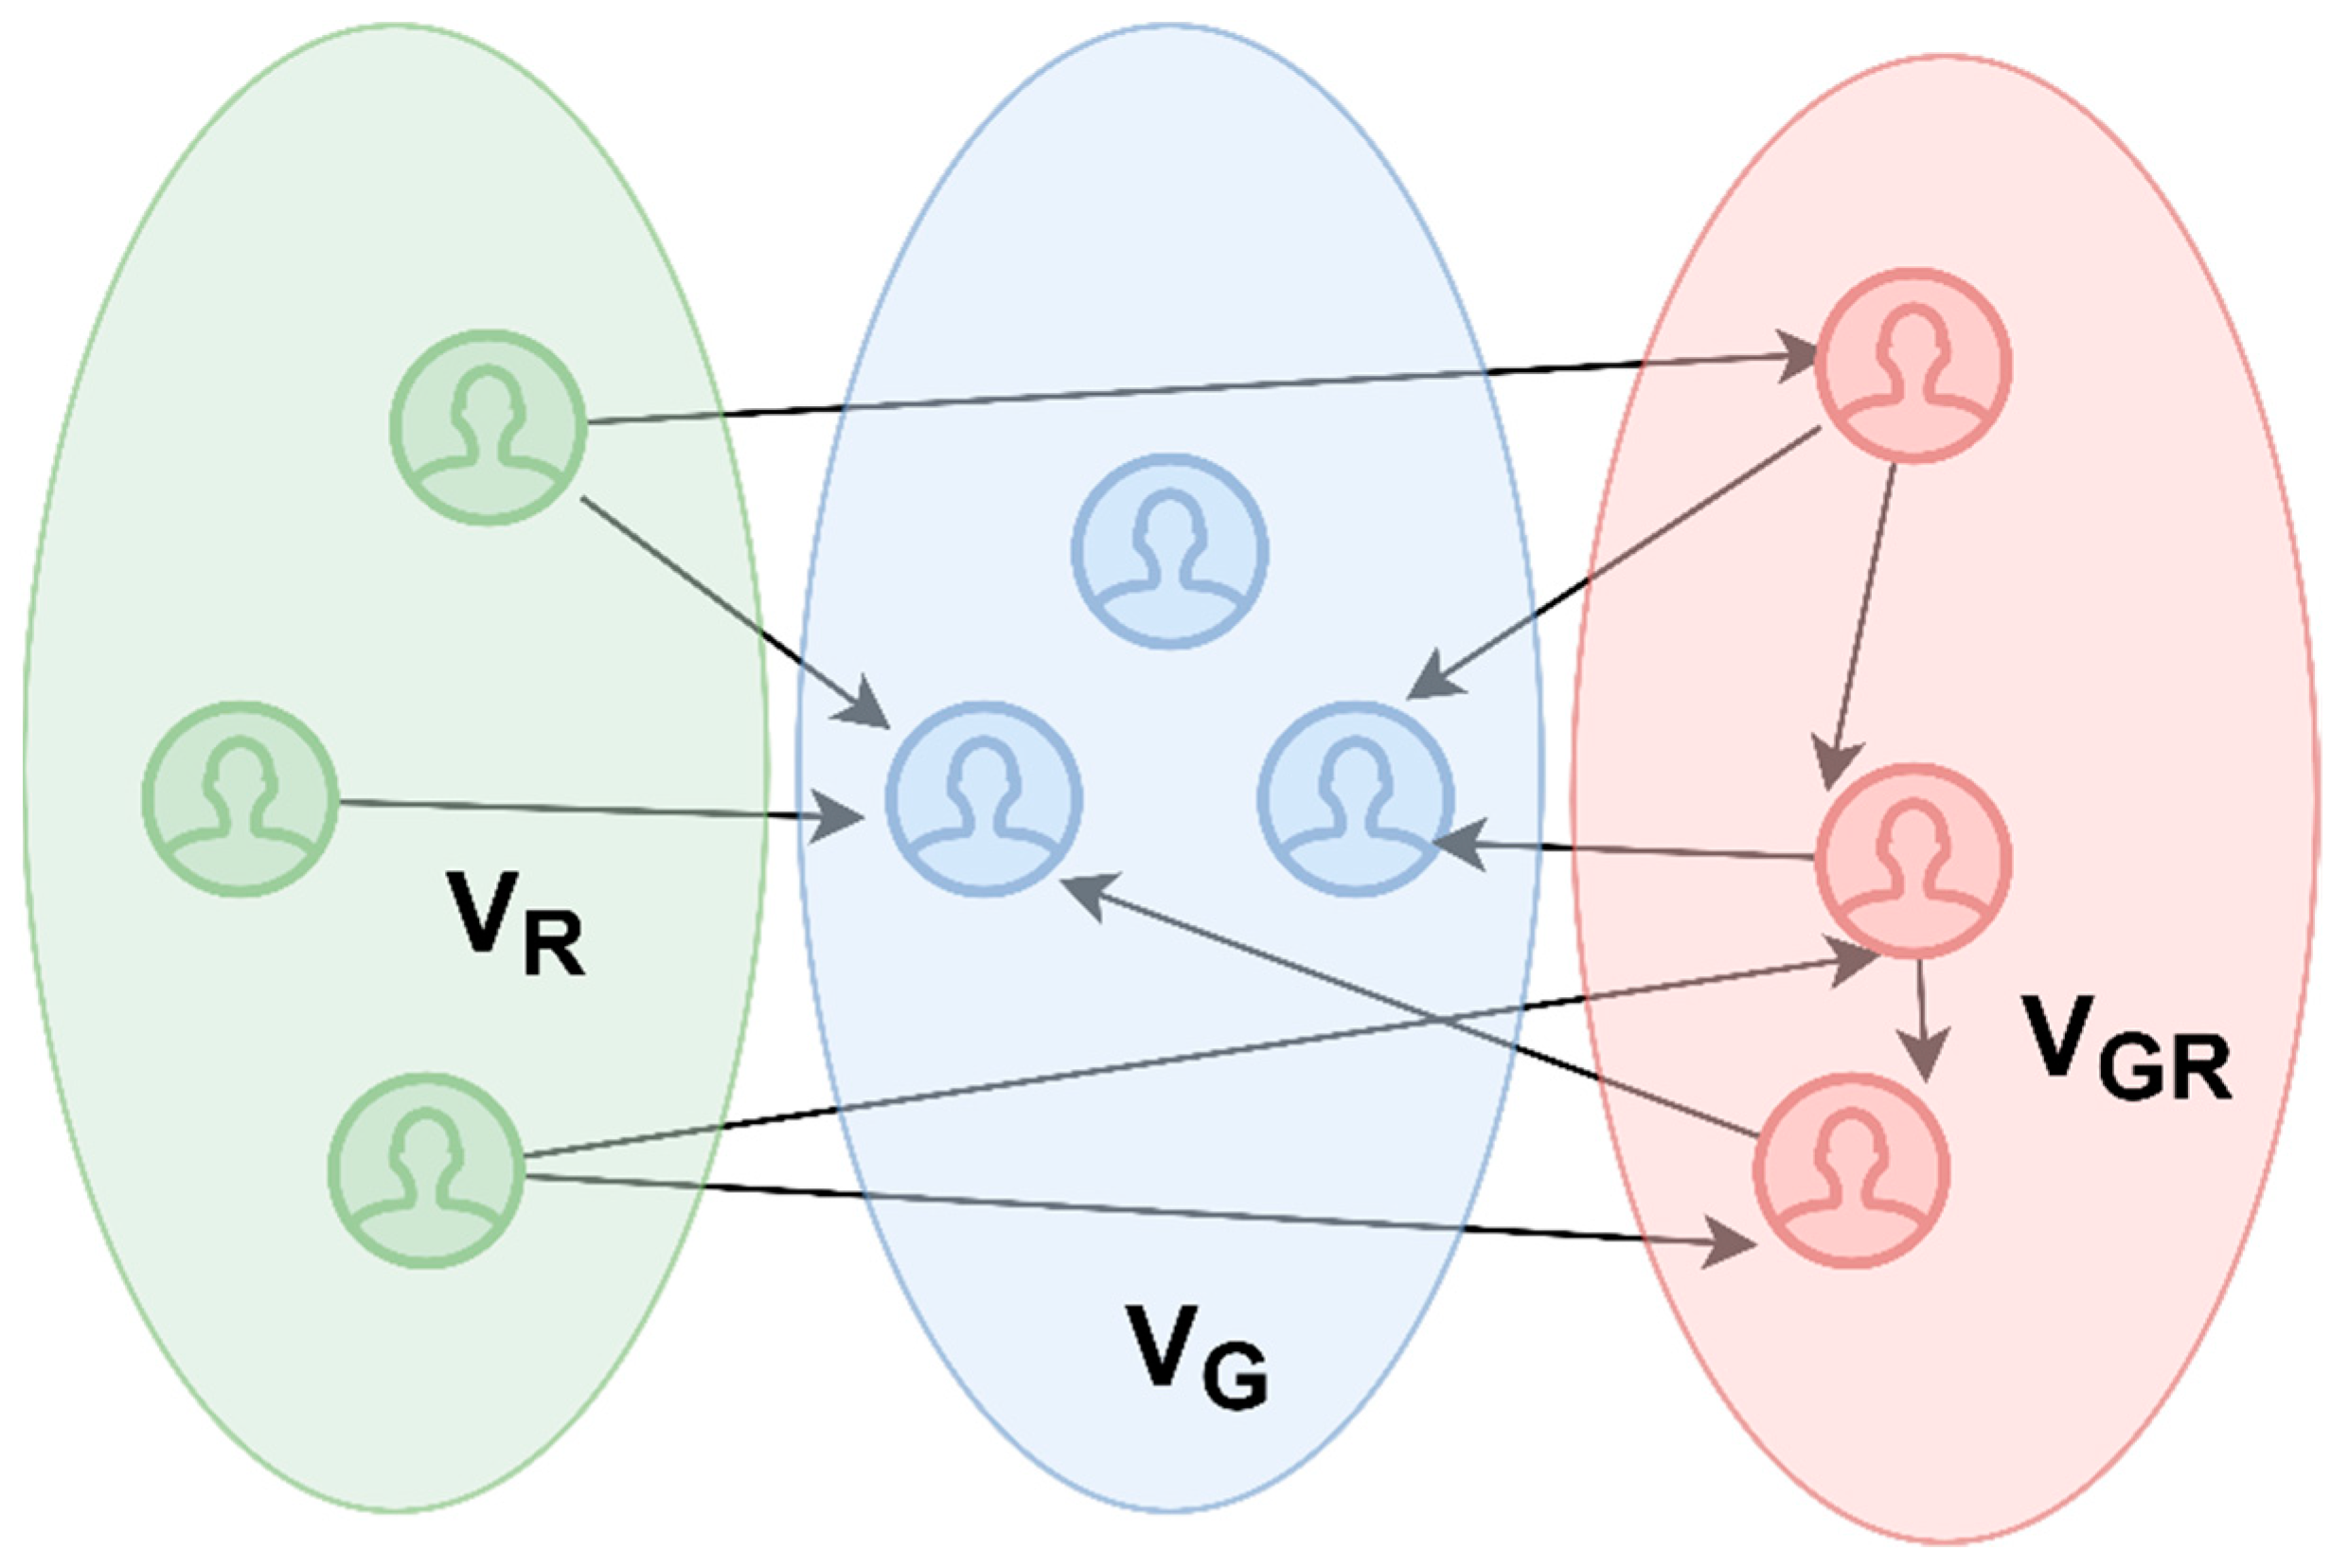
\includegraphics[scale=0.7]{networkedDiscussionRepresentation}
	}
	\caption{Visual representation of the structure of a networked discussion, by user type.}\label{fig:networkedDiscussionRepresentation}
\end{figure}

Let us assume that user \(A\) from \(V_G\) published a message on the social network on some event, and user \(B\) from \(V_R\) reacted to this post via a like, comment, or repost. Then there will be a connection \(B -- A\) (‘\(A\) caused by this publication a reaction from user \(B\)’) in an unweighted directed graph. 

Thus, in this paper, the search for communities in social graphs is the task of analyzing \cref{eqn:51} -- that is, finding sub-structures in a discursive community with three different participation strategies. The methods used for this analysis are discussed below.

\paragraph{3.2. Description of Community Detection Methods} This section will describe clustering techniques that have not yet been applied to \cref{eqn:51}.

\textit{3.2.1. The Directed Louvain Algorithm} Directed Louvain \cite{DuguePerez} is an extension for directed graphs of the greedy Louvain \cite{BlondelGuillaumeLambiotte} algorithm: starting from any set of vertices, the algorithm calculates the increase in modularity from moving vertices between communities. This increase is calculated using the following formula:
\[
	\Delta_{Q_d} = \frac{d^C_i}{m} - \left[\frac{d^{out}_i \cdot \sum_{tot}^{in} + d^{in}_i \sum_{tot}^{out}}{m^2}\right],
\] where \(d^C_i\) -- the degree of node \(i\) in community \(C\); \(d^{in}_i\) \((d^{out}_i)\) -- the indegree (outdegree) of node \(i\); \(sum^{in}_{tot}\) \((\sum_{tot}^{out})\) -- the incoming (outcoming) edges of community \(C\).

\textit{3.2.2. The Leiden Algorithm} The Leiden \cite{TraagWaltmanVanEck} algorithm is partially based on the smart local move algorithm, which can be seen as an improvement on the Louvain \cite{BlondelGuillaumeLambiotte} algorithm, and also uses the idea of speeding up local movement of nodes and the idea of moving nodes to random neighbors. The algorithm can use CPM or modularity as quality functions, and includes three stages:

\begin{enumerate}
	\item Local node movement;
	\item Improving partition;
	\item Enhanced partition-based network aggregation using a non-enhanced partition to
	create an initial partition for the aggregate network.
\end{enumerate}

\textit{3.2.3. The Directed Label Propagation Algorithm} The directed label propagation algorithm (DLPA) \cite{Li} is a development for directed graphs of the label propagation algorithm \cite{RaghavanAlbertKumara} method. LPA is one of the fastest community finding algorithms for undirected graphs. It can be used with large graphs, relies on topology, and is easy to implement:

\begin{enumerate}
	\item The algorithm assigns a unique label to each node;
	\item Each node selects a label among its neighbors based on the frequency of occurrence; 
	\item If the distribution of labels reaches a steady state, the algorithm stops, otherwise it returns to step 2;
\end{enumerate}

The principle of label selection looks like this:
\[
	l^{new}_v = \lvert N^l(v) \rvert,
\]
where \(v\) -- the node, \(l\) -- the node label, and \(N(v)\) -- neighbors of node \(v\).

DLPA differs from the original algorithm by the weighting rule for each edge:
\[
1 - \frac{E^{out}_S E^{in}_T}{k_S k_T}
\]
where \(E^{out}_S\) -- the outdegree of the source node, \(E^{in}_S\) -- the indegree of the target node, \(k_S\) -- the degree of the source node, and \(k_T\) -- the degree of the target node.

\textit{3.2.4. The Infomap Algorithm} The Infomap \cite{RosvallAxelssonBergstrom} algorithm works as follows: each node is assigned to a separate community. Then, in random sequential order, each node is moved to a neighboring com- munity, if this movement decreases the map equation value. The repetition is performed each time in a new random sequential order until no movement leads to a decrease in map equation. Then, the graph is rebuilt, and the communities of the last level are replaced by nodes at this level. Then, the procedure is repeated for this level. The network is rebuilt until the map equation result cannot be reduced any more.

\textit{3.2.5. The Generalized K-Means Algorithm} Generalized K-means using PageRank \cite{HajijSaidTodd} improves the k-means \cite{Lloyd} method, generalizing it to both directed and undirected graphs. Generalized k-means uses the PageRank algorithm as a measure of centrality and the Dijkstra’s algorithm as a metric for the distance between vertices for directed graphs.

Like the usual k-means, this algorithm consists of three stages:

\begin{enumerate}
	\item The initialization stage: k centroid vertices are randomly selected;
	\item The assignment stage: using Voronoi diagrams with centroids to divide the set of vertices into subsets;
	\item The update stage: building subgraphs, calculating PageRank for each subgraph, and updating the centroids.
\end{enumerate}

\textit{3.2.6. The Order Statistics Local Optimization Method} The order statistics local optimization method (OSLOM) \cite{LancichinettiRadicchiRamasco} is based on local optimization of the fitness function, which expresses the statistical significance of clusters in relation to random fluctuations, which is estimated using the extreme and order statistics tools. OSLOM can be used on its own or as a rework procedure for breaks/coverage provided by other methods. The method includes three phases:

\begin{enumerate}
	\item The search for significant clusters before convergence;
	\item Analysis of the resulting set of clusters to detect their internal structure or possible
	associations;
	\item Discovery of the hierarchical structure of clusters.
\end{enumerate}

\textit{3.2.7. The Speaker–Listener Propagation Algorithm} GANXiS, aka SLPA \cite{XieSzymanskiLiu}, is another extension of the LPA \cite{RaghavanAlbertKumara} algorithm that consists of three stages, as described below.

\begin{itemize}
	\item The memory of each node is initialized with the identifier of this node (unique label).
	\item The steps are repeated until the stopping criterion is met:
	\begin{enumerate}
		\item one node is selected as a listener;
		\item each neighbor of the selected node sends one tag following a certain conversation rule, e.g., choosing a random tag from its memory with a probability proportional to the frequency of occurrence of this tag in memory;
		\item the listener accepts a label from a collection of labels received from neighbors following a specific listening rule, e.g., choosing the most popular label from what it has observed at the current stage.
	\end{enumerate}
	\item Finally, post-processing based on in-memory labels of nodes is used to display communities.
\end{itemize}

SLPA utilizes an asynchronous update scheme, i.e., when updating a listener’s memory at time \(t\), some already-updated neighbors have memories of size \(t\) and some other neighbors still have memories of size \(t - 1\). SLPA reduces to LPA when the size of memory is limited to 1, and the stopping criterion is the convergence of all labels. Thus, SLPA is a joint version of the LPA algorithm that is suitable for detecting overlapping (fuzzy) clusters, while the disjoint version of the algorithm may be employed for finding non-fuzzy clusters and is used here for comparative purposes. We will name the joint algorithm GANXiSo, and the disjoint one GANXiSd.

\paragraph{3.3. Evaluation Metrics for Community Detection} In order to evaluate partitions, we decided to use various quality indicators that characterize how similar the structure of connections of a given network is to a community. The metrics are based on the idea that communities are collections of nodes with more connections inside and fewer connections outside. They were selected from a standard set of known metrics, which are commonly used to assess the graph properties of detected communities in a directed graph \cite{Rahman,LeichtNewman,Newman,Fagiolo,ChenNguyenSzymanski,KaurSinghKaushal}. Such properties, for example, include the ability to distinguish large communities in a graph, the density of internal connections within formed communities, the number of edges in a graph outside the community, and the ratio of incoming edges to the total number of community edges. In selecting the metrics, we also used the following logic: (1) the metrics must vary in terms of which graph properties they measure; (2) the metrics have to suit both the density-based and pattern-based clustering; and (3) taken together, the metrics must describe the main graph properties in terms of community detection. The metrics selected have no underlying ‘ground truth’ capacity; that is, none of them can tell whether a hidden community is found or not. However, taken together, the metrics provide for much better clarity on how well the algorithms cluster the graph nodes. The metrics, though, may provide for sociological meaning (e.g., stronger connection of nodes may reveal modularity based on opinion, group belonging, or expression sentiment), but the meaning of the result is task-dependent (e.g., we consider it better when a discussion is less modular, which would mean more equal spread of political opinion). It is not the peculiar sociological meaning that we demand from each metric; taken together, they are to provide for a bigger picture of how close a given algorithm is to finding a closer-to-life number of communities.

\begin{enumerate}
	\item The \textit{NEDindex} \cite{Rahman} value ranges from 0 to 1. Cluster nodes are more strongly con- nected to the entire graph if \textit{NEDindex} tends towards 1, and vice versa, cluster nodes are weakly connected if \textit{NEDindex} is close to 0. \[D(G) = 2 \sum_{1 \le i \le n}e_i,\] \[\textit{NED}(C) = \frac{\lvert V_c \rvert + \lvert E_c \rvert + D(C)}{\lvert V_c \rvert + \begin{pmatrix}
			\lvert V_c \rvert \\
			2 \\
	\end{pmatrix} + D(G,V_c)},\] \begin{equation} 
		\label{eqn:52} 
		\textit{NEDindex} = \sum_{1 \le i \le n} \frac{\textit{NED}(C_i) \cdot D(C_i)}{D(G)}. 
	\end{equation} This metric indicates the strength of the connection between the cluster vertices relative to the entire graph.
	
	\item Directed modularity \cite{LeichtNewman} is an extended version of the modularity metric \cite{Newman} for directed graphs. The higher the value, the better the result. \begin{equation}
		\label{eqn:53} 
		Q = \frac{1}{m} \sum_{ij}\left[A_{ij} - \frac{k^{in}_i k^{out}_j}{m}\right]\delta_{c_ic_j}
	\end{equation} Modularity reflects the concentration of edges within communities compared with random distribution of links between all nodes regardless of communities. Modularity also shows the effectiveness of the method to detect large communities.

	\item Clustering Coefficient is used in this paper as a version of the clustering coefficient \cite{Fagiolo} extended for directed and weighted graphs. \begin{equation}
		\label{eqn:54} 
		C^D = N^{-1} \sum_{i=1}^{N} C_i^D
	\end{equation} In this metric, the average value of the ratio of existing triangles based on the vertex \(i\) to all kinds of triangles based on this vertex is considered, that is, the completeness of the relationship between the vertices is considered. The closer the metric value is to 1, the better the community detection.

	\item Conductance \cite{ChenNguyenSzymanski} is the proportion of the total number of edges outside the commu- nity for unweighted networks or the proportion of the total weight of such edges for weighted networks. This metric allows you to know the “conductivity” of the resulting community. The closer the conductance value to 0, the better the quality of the community. \begin{equation}
		\label{eqn:55}
		\frac{\lvert E_c^{out} \rvert}{\lvert E_c^{in} \rvert + \lvert E_c^{out} \rvert}
	\end{equation}

	\item Contraction \cite{ChenNguyenSzymanski} measures the average number of edges per node within community C or the average weight per node of such edges. This metric shows how important this community is to the rest of the graph. The closer the contraction value to 1, the better the quality of the community. \begin{equation}
		\label{eqn:56}
		\frac{\lvert E_c^{in} \rvert}{c}
	\end{equation}

	\item Expansion \cite{ChenNguyenSzymanski} measures the average number of edges (per node) outside the community C, or the average weight per node of such edges. This metric shows how strongly this community is connected to the rest of the graph. The lower the expansion value, the better the quality of the community.\begin{equation}
		\label{eqn:57}
		\frac{\lvert E_c^{out} \rvert}{c}
	\end{equation}

	\item Community Fitness \cite{KaurSinghKaushal} calculates the ratio of the total indegree number of the community \(C\) to the total degree of \(\alpha\), where is \(\alpha\) a positive number that controls the size of communities. This allows you to find out the density of detected communities. The higher the community fitness value, the better result we get. \begin{equation}
		\label{eqn:58}
		\textit{comfit} = \frac{k_{in}^C}{(k_{in}^C + k_{out}^C)^\alpha}
	\end{equation}
\end{enumerate}

\subsubsection{4. Experiment}

\paragraph{4.1. Experiment Description} The methods suggested above will be applied to the four datasets, after which the resulting values will be evaluated by the metrics~\cref{eqn:52,eqn:53,eqn:54,eqn:55,eqn:56,eqn:57,eqn:58}. For completeness of the experiment, as test data, we take a graph of small size (about 10 thousand nodes), medium size (up to 50 thousand nodes), large size (up to 200 thousand nodes), and extra-large (more than 500 thousand nodes). Moving from a small dataset to large ones during testing, algorithms and metrics that do not perform efficiently on the task will be cut off. Next, two tables will be created for each dataset. The first table will contain the results of applying the metrics, highlighting the best results in each metric. The second table will contain the count of resulting clusters and the size of the seven largest of them. Based on the data obtained for each dataset, it will be possible to draw a conclusion on efficiency of the algorithms on the datasets of varying volume.

Our strategy differs from the ‘ground truth’ one: instead of having just one pre- analyzed discussion with known modularity as a ‘ground truth’ (which might lead to the situation of random closeness of this or that model to the content-based graph modularity), we take four discussions on various volume and set the sociological perspective for expectations, to see which algorithm(s) come closer to them on datasets of varying volume. This is why our design implies use of multiple metrics and multiple datasets.

\paragraph{4.2. The Datasets} To test and evaluate the extant tools, real-world datasets crawled from Twitter, a microblogging service with elements of a social network, were used. Each of these datasets was collected using the Twitter API during or immediately after high-profile, socially resonant events that triggered social unrest \cite{BodrunovaBlekanovSmoliarova,BodrunovaLitvinenkoBlekanov,BodrunovaBlekanov}. For accurate results, the datasets vary in size (the number of tweets), and testing will be carried out from the smallest to the largest one.

The mall size dataset (hereinafter referred to as “Biryulevo”) consists of the tweets posted on 17 to 31 October 2013, during the sharp phase of the riots in the Moscow district Biryulevo-Zapadnoe. Initially, it contains 20,106 links and 11,429 users, but, after cleaning from isolate users, 10,275 vertices and 20,093 edges remain.

The medium size dataset (hereinafter referred to as “Cologne”) contains the data collected for 1 to 31 January 2016, within the discussion on mass attacks on women in Cologne on the eve of 2016. Initially, it contained 40,117 users and 98,508 links, after cleaning from isolate users, the number of users decreased to 36,850, and the number of links to 96,244.

The large size dataset (hereinafter referred to as “Ferguson”) contains data from 22 to 31 August 2014, on the riots in Ferguson, USA, provoked by a murder of an African Ameri- can teenager by a white policeman. The dataset contains 169,676 users with 334,050 links, and, after cleaning from isolate users, 143,024 users with 325,369 links remain.

The extra-large dataset (hereinafter referred to as “Charlie Hebdo”) was obtained for the period of 7 to 10 January 2015 by collecting a response to a terrorist attack in the editorial office of the Charlie Hebdo magazine. The total number of participants is 719,503, connections are 981,131, and, after clearing, there are 617,041 users and 980,351 connections.

\subsubsection{5. Results}

As stated above, in this section we present the results of the experiment for four various datasets of different volumes.

The results of the task solution for the Biryulevo case are shown in Tables~\cref{tab:biryulevoMetricsEvaluation} and~\cref{tab:biryulevoCommunityNumber}. Each method has its own peculiarities:

\begin{itemize}
	\item The Infomap algorithm tends to highlight one large community, which can be used as a starting point for deeper research;
	\item Similar to the Infomap algorithm, GANXiS (both pure and overlapping versions) distinguishes one large society, but this set is smaller than for Infomap;
	\item The generalized K-means algorithm does not take into account the lack of connections between isolates, which is the reason for the unification of almost all small discussions (2-3-4 participants) into one large society;
	\item Directed Louvain shows good results. However, it was not able to get ahead in any metric, steadily holding on to the second or third place;
	\item Despite it only partially belonging to the directed graph clustering algorithms, Leiden (both the one that uses modularity and the one that uses the clique percolation method) shows good results, being ahead of the directed Louvain algorithm in almost every point. Its peculiarity is that it highlights the communities of average size and/or close to each other in size;
	\item DLPA allocates almost twice as many communities as other algorithms, all but the largest do not differ much in size;
	\item OSLOM identifies a large number of communities, which, moreover, can strongly overlap. 
\end{itemize}

\begin{table}[ht]%
	\centering
	\caption{Results of evaluations by metrics on the Biryulevo dataset.}%
	\label{tab:biryulevoMetricsEvaluation}% label всегда желательно идти после caption
	\begin{adjustbox}{width=1\textwidth}
		\small
		\begin{tabular}{ c  c  c  c  c  c  c  c }% Вертикальные полосы не используются принципиально, как и лишние горизонтальные (допускается по ГОСТ 2.105 пункт 4.4.5) % @{} позволяет прижиматься к краям
			\toprule
			& DirMod & ClusCoe & ComFit & NEDind & Conduc & Contrac & Expans\\
			\hline
			DLPA & 0.486 & \textbf{0.056} & 1.373 & 0.605 & 0.625 & \textbf{0.849} & 2.361 \\
			DirLouv & 0.574 & 0.039 & 6.548 & 0.793 & 0.286 & 0.766 & 0.715\\
			Infomap & 0.088 & 0.034 & 7.877 & \textbf{0.940} & \textbf{0.209} & 0.685 & \textbf{0.375}\\
			OSLOM & -- & 0.035 & 2.479 & 0.501 & 0.967 & 0.087 & 1.403 \\
			GKM & 0.390 & 0.0099 & 7.956 & 0.423 & 0.950 & 0.190 & 2.161 \\
			LeidMod & \textbf{0.584} & 0.039 & 6.686 & 0.806 & 0.278 & 0.761 & 0.686 \\
			LeidCPM & 0.571 & 0.040 & 5.052 & 0.676 & 0.365 & 0.828 & 1.001 \\
			GANXiSd & 0.406 & 0.040 & 2.538 & 0.661 & 0.526 & 0.841 & 1.681\\
			GANXiSo & -- & 0.049 & 3.295 & 0.643 & 0.550 & 0.848 & 2.282 \\
			\bottomrule
			\multicolumn{8}{@{}p{\textwidth}}{%
				\hspace*{2.5em}% абзацный отступ - требование ГОСТ 2.105
				Note. The best results are highlighted in bold.
			}\\
		\end{tabular}%
	\end{adjustbox}
\end{table}

\begin{table}[ht]%
	\centering
	\caption{The number of communities obtained on the Biryulevo dataset and the value of the seven largest of them for each algorithm.}%
	\label{tab:biryulevoCommunityNumber}% label всегда желательно идти после caption
%	\begin{adjustbox}{width=1\textwidth}
%		\small
		\begin{tabular}{ c  c  c  c  c  c  c  c  c }% Вертикальные полосы не используются принципиально, как и лишние горизонтальные (допускается по ГОСТ 2.105 пункт 4.4.5) % @{} позволяет прижиматься к краям
			\toprule
			& Count & 1 & 2 & 3 & 4 & 5 & 6 & 7\\
			\hline
			DLPA & 1159 & 741 & 205 & 171 & 115 & 111 & 108 & 105 \\
			DirLouv & 243 & 691 & 583 & 494 & 486 & 463 & 459 & 381 \\
			Infomap & 202 & 9276 & 232 & 86 & 41 & 33 & 28 & 26 \\
			OSLOM & 642 & 2637 & 1743 & 1425 & 847 & 763 & 737 & 619\\
			GKM & 200 & 3300 & 2815 & 1812 & 815 & 496 & 313 & 90 \\
			LeidMod & 238 & 716 & 464 & 458 & 451 & 416 & 388 & 356\\
			LeidCPM & 315 & 627 & 613 & 226 & 226 & 214 & 208 & 208 \\
			GANXiSd & 627 & 4881 & 190 & 146 & 129 & 113 & 103 & 101 \\
			GANXiSo & 647 & 4956 & 638 & 255 & 166 & 146 & 139 & 83 \\
			\bottomrule
		\end{tabular}%
%	\end{adjustbox}
\end{table}

The results for the Cologne case are shown in Tables~\cref{tab:cologneMetricsEvaluation} and~\cref{tab:cologneCommunityNumber}. At this dataset volume,~\cref{eqn:53} metric showed high computational complexity, so it was no longer used.

\begin{table}[ht]%
	\centering
	\caption{Results of evaluations by metrics on the Cologne dataset.}%
	\label{tab:cologneMetricsEvaluation}% label всегда желательно идти после caption
	\begin{adjustbox}{width=1\textwidth}
		\small
		\begin{tabular}{ c  c  c  c  c  c  c  c }% Вертикальные полосы не используются принципиально, как и лишние горизонтальные (допускается по ГОСТ 2.105 пункт 4.4.5) % @{} позволяет прижиматься к краям
			\toprule
			& DirMod & ClusCoe & ComFit & NEDind & Conduc & Contrac & Expans\\
			\hline
			DLPA & -- & \textbf{0.070} & 2.299 & 0.723 & 0.521 & 0.815 & 1.378 \\
			DirLouv & -- & 0.028 & 7.753 & 0.917 & 0.234 & 0.691 & 0.459 \\
			Infomap & -- & 0.024 & 8.468 & \textbf{0.949} & \textbf{0.201} & 0.653 & \textbf{0.344}\\
			OSLOM & -- & 0.034 & 3.380 & 0.495 & 0.963 & 0.098 & 1.249 \\
			GKM & -- & 0.013 & \textbf{28.498} & 0.422 & 0.934 & 0.209 & 2.600 \\
			LeidMod & -- & 0.028 & 7.764 & 0.916 & 0.233 & 0.693 & 0.459 \\
			LeidCPM & -- & 0.033 & 4.379 & 0.689 & 0.397 & 0.793 & 1.030 \\
			GANXiSd & -- & 0.031 & 3.057 & 0.693 & 0.501 & 0.807 & 1.798 \\
			GANXiSo & -- & 0.042 & 3.551 & 0.670 & 0.526 & \textbf{0.829} & 2.290 \\
			\bottomrule
			\multicolumn{8}{@{}p{\textwidth}}{%
				\hspace*{2.5em}% абзацный отступ - требование ГОСТ 2.105
				Note. The best results are highlighted in bold.
			}\\
		\end{tabular}%
	\end{adjustbox}
\end{table}

\begin{table}[ht]%
	\centering
	\caption{The number of communities obtained on the Cologne dataset and the value of the seven largest of them for each algorithm.}%
	\label{tab:cologneCommunityNumber}% label всегда желательно идти после caption
%	\begin{adjustbox}{width=1\textwidth}
%		\small
		\begin{tabular}{ c  c  c  c  c  c  c  c  c }% Вертикальные полосы не используются принципиально, как и лишние горизонтальные (допускается по ГОСТ 2.105 пункт 4.4.5) % @{} позволяет прижиматься к краям
			\toprule
			& Count & 1 & 2 & 3 & 4 & 5 & 6 & 7\\
			\hline
			DLPA & 2479 & 20,669 & 425 & 277 & 249 & 198 & 173 & 168 \\
			DirLouv & 735 & 4356 & 4105 & 4091 & 3604 & 3447 & 1933 & 1886  \\
			Infomap & 673 & 27,016 & 3726 & 1145 & 590 & 465 & 445 & 338 \\
			OSLOM & 1690 & 10,823 & 7336 & 3058 & 1881 & 1519 & 1466 & 921 \\
			GKM & 200 & 11,474 & 7737 & 4353 & 2971 & 2947 & 1859 & 1119  \\
			LeidMod & 734 & 4453 & 3882 & 3540 & 3212 & 3181 & 2686 & 1739 \\
			LeidCPM & 1221 & 2395 & 672 & 625 & 414 & 405 & 362 & 355 \\
			GANXiSd & 1864 & 24,911 & 128 & 110 & 108 & 94 & 89 & 80 \\
			GANXiSo & 1964 & 25,365 & 458 & 210 & 162 & 128 & 110 & 83 \\
			\bottomrule
		\end{tabular}%
%	\end{adjustbox}
\end{table}

For the mid-range dataset, the algorithms have shown the following results:

\begin{itemize}
	\item Infomap showed a more even selection of communities than on the Biryulevo dataset, nevertheless retaining the emphasis on the largest of them;
	\item GANXiS continued to highlight one large community, and the emphasis on this community grew;
	\item As in the case of the Biryulevo dataset, generalized K-means has combined minor discussions into one large group;
	Directed Louvain performed well again, continuing to hold on to second or third place;
	\item Unlike for the first dataset, the sizes of communities after the Leiden algorithm differ depending on the metric (CPM or modularity). The first option showed a large number of fairly small communities, while the second showed a smaller number of moderately large communities;
	\item DLPA on the Cologne dataset showed the risk of going into “overflow” of one community, not giving any other one chances to grow while, again, having twice as many	communities as other algorithms;
	\item OSLOM distinguished communities of not the best quality even in comparison with	GANXiS.
\end{itemize}

The results for the large dataset (Tables~\cref{tab:fergusonMetricsEvaluation} and~\cref{tab:fergusonCommunityNumber}) may be described the following way:

\begin{itemize}
	\item Infomap once again got four best metrics results, receiving, though, one large community;
	\item GANXiS kept the trend shown on small and medium datasets;
	\item The generalized K-Means algorithm has shown its inapplicability to sufficiently perform on large graphs, since both the computational cost and the memory cost made it impossible to use this algorithm;
	\item Directed Louvain retains its position relative to other algorithms;
	\item The Leiden algorithm kept the trend shown on the medium-sized dataset;
	\item DLPA identified more equal-sized communities than on the medium dataset, which demonstrates variability of the algorithm performance depending on the size of initial data;
	\item OSLOM got results worse than on medium dataset on every, except metric (8).
\end{itemize}

\begin{table}[ht]%
	\centering
	\caption{Results of evaluations by metrics on the Ferguson dataset.}%
	\label{tab:fergusonMetricsEvaluation}% label всегда желательно идти после caption
	\begin{adjustbox}{width=1\textwidth}
		\small
		\begin{tabular}{ c  c  c  c  c  c  c  c }% Вертикальные полосы не используются принципиально, как и лишние горизонтальные (допускается по ГОСТ 2.105 пункт 4.4.5) % @{} позволяет прижиматься к краям
			\toprule
			& DirMod & ClusCoe & ComFit & NEDind & Conduc & Contrac & Expans\\
			\hline
			DLPA & -- & \textbf{0.085} & 1.522 & 0.640 & 0.599 & \textbf{0.847} & 2.735 \\
			DirLouv & -- & 0.027 & 6.318 & 0.949 & 0.208 & 0.666 & 0.371 \\
			Infomap & -- & 0.026 & \textbf{6.476} & \textbf{0.959} & \textbf{0.199} & 0.655 & \textbf{0.340}\\
			OSLOM & -- & 0.034 & 2.426 & 0.493 & 0.964 & 0.096 & 1.305 \\
			GKM & -- & -- & -- & -- & -- & -- & -- \\
			LeidMod & -- & 0.027 & 6.244 & 0.945 & 0.212 & 0.670 & 0.380 \\
			LeidCPM & -- & 0.035 & 4.494 & 0.740 & 0.345 & 0.782 & 1.062 \\
			GANXiSd & -- & 0.031 & 3.303 & 0.772 & 0.422 & 0.773 & 1.260 \\
			GANXiSo & -- & 0.034 & 4.064 & 0.779 & 0.397 & 0.756 & 1.294 \\
			\bottomrule
			\multicolumn{8}{@{}p{\textwidth}}{%
				\hspace*{2.5em}% абзацный отступ - требование ГОСТ 2.105
				Note. The best results are highlighted in bold.
			}\\
		\end{tabular}%
	\end{adjustbox}
\end{table}

\begin{table}[ht]%
	\centering
	\caption{The number of communities obtained on the Ferguson dataset and the value of the seven largest of them for each algorithm.}%
	\label{tab:fergusonCommunityNumber}% label всегда желательно идти после caption
%	\begin{adjustbox}{width=1\textwidth}
%		\small
		\begin{tabular}{ c  c  c  c  c  c  c  c  c }% Вертикальные полосы не используются принципиально, как и лишние горизонтальные (допускается по ГОСТ 2.105 пункт 4.4.5) % @{} позволяет прижиматься к краям
			\toprule
			& Count & 1 & 2 & 3 & 4 & 5 & 6 & 7\\
			\hline
			DLPA & 18,389 & 3059 & 1224 & 1044 & 913 & 877 & 708 & 662 \\
			DirLouv & 4429 & 16,029 & 13,916 & 13,391 & 12,936 & 8827 & 4334 & 4053 \\
			Infomap & 4321 & 106,521 & 15,617 & 1651 & 1012 & 506 & 409 & 353\\
			OSLOM & 11,546 & 16,417 & 15,372 & 10,438 & 8874 & 6587 & 4081 & 3074 \\
			GKM & -- & -- & -- & -- & -- & -- & -- & -- \\
			LeidMod & 4481 & 15,804 & 12,715 & 12,212 & 11,385 & 9162 & 4355 & 4260 \\
			LeidCPM & 6226 & 1001 & 729 & 704 & 648 & 572 & 554 & 531 \\
			GANXiSd & 8472 & 98,344 & 211 & 184 & 159 & 104 & 100 & 97 \\
			GANXiSo & 7489 & 111,798 & 184 & 159 & 155 & 102 & 95 & 84\\
			\bottomrule
		\end{tabular}%
%	\end{adjustbox}
\end{table}

The results for the extra-large dataset (Tables~\cref{tab:charlieHebdoMetricsEvaluation} and~\cref{tab:charlieHebdoMetricsEvaluation}) are the following:

\begin{itemize}
	\item Infomap showed a better division into same-size communities, retaining the emphasis on the largest of them;
	\item It revealed that the GANXiS algorithm is not applicable to extra-large networks;
	\item As in the case of the large dataset, generalized K-means is not applicable to the networks of this size;
	\item The directed Louvain continued to evenly allocate communities;
	\item Leiden shown dramatically grown difference between the size of CPM and modularity metric-based communities;
	\item DLPA on an extra-large dataset has allocated a lot of small, smaller than before, communities;
	\item OSLOM has got even worse results than on the large dataset on every metric.
	
\end{itemize}

\begin{table}[ht]%
	\centering
	\caption{Results of evaluations by metrics on the Charlie Hebdo dataset.}%
	\label{tab:charlieHebdoMetricsEvaluation}% label всегда желательно идти после caption
	\begin{adjustbox}{width=1\textwidth}
		\small
		\begin{tabular}{ c  c  c  c  c  c  c  c }% Вертикальные полосы не используются принципиально, как и лишние горизонтальные (допускается по ГОСТ 2.105 пункт 4.4.5) % @{} позволяет прижиматься к краям
			\toprule
			& DirMod & ClusCoe & ComFit & NEDind & Conduc & Contrac & Expans\\
			\hline
			DLPA & -- & \textbf{0.027} & 1.375 & 0.672 & 0.514 & \textbf{0.764} & 1.550 \\
			DirLouv & -- & 0.012 & 4.395 & 0.953 & 0.163 & 0.604 & 0.256 \\
			Infomap & -- & 0.012 & 4.381 & 0.942 & 0.166 & 0.608 & 0.268 \\
			OSLOM & -- & 0.015 & 1.730 & 0.479 & 0.979 & 0.054 & 1.239 \\
			GKM & -- & -- & -- & -- & -- & -- & -- \\
			LeidMod & -- & 0.011 & \textbf{4.408} & \textbf{0.955} & \textbf{0.162} & 0.054 & 1.239 \\
			LeidCPM & -- & 0.016 & 3.351 & 0.758 & 0.276 & 0.713 & 0.663 \\
			GANXiSd & -- & -- & -- & -- & -- & -- & --  \\
			GANXiSo & -- & -- & -- & -- & -- & -- & --  \\
			\bottomrule
			\multicolumn{8}{@{}p{\textwidth}}{%
				\hspace*{2.5em}% абзацный отступ - требование ГОСТ 2.105
				Note. The best results are highlighted in bold.
			}\\
		\end{tabular}%
	\end{adjustbox}
\end{table}

\begin{table}[ht]%
	\centering
	\caption{The number of communities obtained on the Charlie Hebdo dataset and the value of the seven largest of them for each algorithm.}%
	\label{tab:charlieHebdoCommunityNumber}% label всегда желательно идти после caption
%	\begin{adjustbox}{width=1\textwidth}
%		\small
		\begin{tabular}{ c  c  c  c  c  c  c  c  c }% Вертикальные полосы не используются принципиально, как и лишние горизонтальные (допускается по ГОСТ 2.105 пункт 4.4.5) % @{} позволяет прижиматься к краям
			\toprule
			& Count & 1 & 2 & 3 & 4 & 5 & 6 & 7\\
			\hline
			DLPA & 84,409 & 1244 & 882 & 726 & 662 & 576 & 529 & 488  \\
			DirLouv & 26,415 & 68,217 & 45,678 & 44,734 & 40,369 & 26,807 & 22,583 & 18,774 \\
			Infomap & 26,497 & 164,839 & 33,635 & 32,111 & 25,038 & 20,098 & 17,226 & 14,033 \\
			OSLOM & 67,296 & 34,960 & 27,735 & 26,061 & 17,319 & 10,912 & 7614 & 6962 \\
			GKM & -- & -- & -- & -- & -- & -- & -- & -- \\
			LeidMod & 26,335 & 56,201 & 39,371 & 33,976 & 27,120 & 25,745 & 20,270 & 17,705 \\
			LeidCPM & 34,647 & 949 & 719 & 626 & 607 & 565 & 531 & 521 \\
			GANXiSd & -- & -- & -- & -- & -- & -- & -- & -- \\
			GANXiSo & -- & -- & -- & -- & -- & -- & -- & -- \\
			\bottomrule
		\end{tabular}%
%	\end{adjustbox}
\end{table}

\subsubsection{6. Discussion and Conclusions}

The experiments conducted have shown the relative mathematical efficiency of the selected methods for detecting user communities in the discussions of Twitter (the mi- croblogging service with elements of a social network) when the discussions are presented in the form of directed graphs of different sizes. Table~\cref{tab:modelSummaryEvaluation} clearly demonstrates that the Infomap algorithm can be called the best; however, due to the property of highlighting one large society, it can rather be used as a preparatory stage for the subsequent clustering by another algorithm, or the repeated application of Infomap. After Infomap comes the Leiden algorithm, which has shown the best results after Infomap, and does not have the ability to single out one large community. Therefore, these two algorithms can be used in conjunction. If it is necessary to isolate overlapping communities based on test results, the GANXiS algorithm should be used.

\begin{longtblr}[
	caption = {Results of evaluations by metrics on the Charlie Hebdo dataset.},
	label = {tab:modelSummaryEvaluation},
	remark{\hspace*{2.5em}Note} = {The best results for each case/algorithm are highlighted in bold.},
	]{
		colspec = {XXXXX}, 
		width = 1.0\linewidth,
		rowhead = 1,
	} 
			\toprule
			& Bir & Col & Fer & ChE \\
			\hline
			\SetCell[c=5]{c}DirMod \\
			\hline
			DLPA & 0.486 & -- & -- & -- \\
			DirLouv & 0.574 & -- & -- & --\\
			Infomap & 0.088 & -- & -- & --\\
			OSLOM & -- & -- & --  & --\\
			GKM & -- & -- & -- & --\\
			LeidMod & 0.39 & -- & -- & -- \\
			LeidCPM & \textbf{0.584} & -- & -- & --\\
			GANXiSd & 0.406 & -- & -- & -- \\
			GANXiSo & -- & -- & -- & -- \\
			\hline
			\SetCell[c=5]{c}ClusCoe \\
			\hline
			DLPA & \textbf{0.056} & \textbf{0.07} & \textbf{0.085} & \textbf{0.027} \\
			DirLouv & 0.039 & 0.028 & 0.027 & 0.012 \\
			Infomap & 0.034 & 0.024 & 0.026 & 0.012 \\
			OSLOM & 0.035 & 0.034 & 0.034 & 0.015\\
			GKM & 0.0099 & -- & -- & --\\
			LeidMod & 0.039 & 0.028 & 0.027 & 0.011 \\
			LeidCPM & 0.04 & 0.033 & 0.035 & 0.016 \\
			GANXiSd & 0.04 & 0.031 & 0.031 & -- \\
			GANXiSo & 0.049 & 0.042 & 0.034 & -- \\
			\hline
			\SetCell[c=5]{c}ComFit \\
			\hline
			DLPA & 1.373 & 2.299 & 1.522 & 1.375 \\
			DirLouv & 6.548 & 7.753 & 6.318 & 4.395 \\
			Infomap & 7.877 & 8.468 & \textbf{6.476} & 4.381\\
			OSLO & 2.479 & 3.38 & 2.426 & 1.73 \\
			GKM & \textbf{7.956} & \textbf{28.498} & -- & --\\
			LeidMod & 6.686 & 7.764 & 6.244 & \textbf{4.408} \\
			LeidCPM & 5.052 & 4.379 & 4.494 & 3.351 \\
			GANXiSd & 2.538 & 3.057 & 3.303 & -- \\
			GANXiSo & 3.295 & 3.551 & 4.064 & -- \\
			\hline
			\SetCell[c=5]{c}NEDind \\
			\hline
			DLPA & 0.605 & 0.723 & 0.64 & 0.672 \\
			DirLouv & 0.793 & 0.917 & 0.949 & 0.953 \\
			Infomap & \textbf{0.94} & \textbf{0.949} & \textbf{0.959} & 0.942 \\
			OSLO & 0.501 & 0.495 & 0.493 & 0.479 \\
			GKM & 0.423 & 0.422 & -- & --\\
			LeidMod & 0.806 & 0.916 & 0.945 & \textbf{0.955}  \\
			LeidCPM & 0.67 &6 0.689 & 0.74 & 0.758  \\
			GANXiSd & 0.661 & 0.693 & 0.772 & -- \\
			GANXiSo & 0.643 & 0.67 & 0.799 & -- \\
			\hline
			\SetCell[c=5]{c}Conduc \\
			\hline
			DLPA & 0.625 & 0.521 & 0.599 & 0.514 \\
			DirLouv & 0.286 & 0.234 & 0.208 & 0.163 \\
			Infomap & \textbf{0.209} & \textbf{0.201} & \textbf{0.199} & 0.166 \\
			OSLO & 0.967 & 0.963 & 0.964 & 0.979 \\
			GKM & 0.95 & 0.934 & -- & --\\
			LeidMod & 0.278 & 0.233 & 0.212 & \textbf{0.162} \\
			LeidCPM & 0.365 & 0.397 & 0.345 & 0.276  \\
			GANXiSd & 0.526 & 0.501 & 0.422 & -- \\
			GANXiSo & 0.55 & 0.526 & 0.397 & -- \\
			\hline
			\SetCell[c=5]{c}Contrac \\
			\hline
			DLPA & \textbf{0.849} & 0.815 & \textbf{0.847} & \textbf{0.764} \\
			DirLouv & 0.766 & 0.691 & 0.666 & 0.604  \\
			Infomap & 0.685 & 0.653 & 0.655 & 0.608  \\
			OSLO & 0.08 &7 0.098 & 0.096 & 0.054  \\
			GKM & 0.19 & 0.209 & -- & --\\
			LeidMod & 0.761 & 0.693 & 0.67 & 0.603 \\
			LeidCPM & 0.828 & 0.793 & 0.782 & 0.713   \\
			GANXiSd & 0.841 & 0.807 & 0.773 & -- \\
			GANXiSo & 0.848 & \textbf{0.829} & 0.756 & -- \\
			\hline
			\SetCell[c=5]{c}Expans \\
			\hline
			DLPA & 2.361 & 1.378 & 2.735 & 1.55\\
			DirLouv & 0.715 & 0.459 & 0.371 & 0.256\\
			Infomap & \textbf{0.375} & \textbf{0.344} & \textbf{0.34} & 0.268   \\
			OSLO & 1.403 & 1.249 & 1.305 & 1.239   \\
			GKM & 2.161 & 2.6 & -- & --\\
			LeidMod & 0.686 & 0.459 & 0.38 & \textbf{0.253}  \\
			LeidCPM & 1.001 & 1.030 & 1.062 & 0.663  \\
			GANXiSd & 1.681 & 1.798 & 1.26 & -- \\
			GANXiSo & 2.282 & 2.290 & 1.294 & -- \\
			\bottomrule
%		\end{tabular}%
%	\end{adjustbox}
\end{longtblr}

Table~\cref{tab:communitiesObtained} shows that the generalized K-means and GANXiS algorithms are not suitable for large-scale Twitter data. Infomap and Leiden (again), just as Direct Louvain, show very similar results as to the number of the detected communities, and the numbers are lower. Here, we need to repeat that, without a clear sociological task, we could not set the ground truth to which to compare the test results; the number of the detected communities (higher or lower) is better depending on the research goal. In general, the low number of robust communities is optimal. This is why we see these three algorithms as coming closer to possible ground truth in social research. Yet, it is also necessary to state that algorithmic results do not correspond to the logic of social studies designated in Section 2.2, as the methods come to either delineation of one large community or a much larger number of smaller communities detected. Of the three aforementioned algorithms with the best (lowest) number of communities, Infomap finds the largest groups, which might be considered the best result.

\begin{table}[ht]%
	\centering
	\caption{The number of communities obtained as compared by algorithm and the seven largest communities, summary table.}%
	\label{tab:communitiesObtained}% label всегда желательно идти после caption
	\begin{adjustbox}{width=1\textwidth}
		\small
		\begin{tabular}{ c  c  c  c  c  c  c  c  c  c  }% Вертикальные полосы не используются принципиально, как и лишние горизонтальные (допускается по ГОСТ 2.105 пункт 4.4.5) % @{} позволяет прижиматься к краям
			\toprule
			Algorithm & Case & Count & 1 & 2 & 3 & 4 & 5 & 6 & 7 \\
			\hline
			\multirow{4}{*}{DLPA} & Bir & 1159 & 741 & 205 & 171 & 115 & 111 & 108 & 105 \\
			& Col & 2479 & 20,669 & 425 & 277 & 249 & 198 & 173 & 168 \\
			& Fer & 18,389 & 3059 & 1224 & 1044 & 913 & 877 & 708 & 662\\
			& ChE & 84,409 & 1244 & 882 & 726 & 662 & 576 & 529 & 488 \\
			\hline
			\multirow{4}{*}{DirLouv} & Bir & 243 & 691 & 583 & 494 & 486 & 463 & 459 & 381 \\
			& Col & 735 & 4356 & 4105 & 4091 & 3604 & 3447 & 1933 & 1886 \\
			& Fer & 4429 & 16,029 & 13,916 & 13,391 & 12,936 & 8827 & 4334 & 4053 \\
			& ChE & 26,415 & 68,217 & 45,678 & 44,734 & 40,369 & 26,807 & 22,583 & 18,774 \\
			\hline
			\multirow{4}{*}{Infomap} & Bir & 202 & 9276 & 232 & 86 & 41 & 33 & 28 & 26 \\
			& Col & 673 & 27,016 & 3726 & 1145 & 590 & 465 & 445 & 338 \\
			& Fer & 4321 & 106,521 & 15,617 & 1651 & 1012 & 506 & 409 & 353 \\
			& ChE & 26,497 & 164,839 & 33,635 & 32,111 & 25,038 & 20,098 & 17,226 & 14,033 \\
			\hline
			\multirow{4}{*}{OSLOM} & Bir & 642 & 2637 & 1743 & 1425 & 847 & 763 & 737 & 619 \\
			& Col & 1690 & 10,823 & 7336 & 3058 & 1881 & 1519 & 1466 & 921 \\
			& Fer & 11,546 & 16,417 & 15,372 & 10,438 & 8874 & 6587 & 4081 & 3074 \\
			& ChE & 67,296 & 34,960 & 27,735 & 26,061 & 17,319 & 10,912 & 7614 & 6962 \\
			\hline
			\multirow{4}{*}{GKM} & Bir & 200 & 3300 & 2815 & 1812 & 815 & 496 & 313 & 90 \\
			& Col & 200 & 11,474 & 7737 & 4353 & 2971 & 2947 & 1859 & 1119 \\
			& Fer & --& --& --& --& --& --& --& --\\
			& ChE & --& --& --& --& --& --& --& --\\
			\hline
			\multirow{4}{*}{LeidMod} & Bir & 238 & 716 & 464 & 458 & 451 & 416 & 388 & 356\\
			& Col & 734 & 4453 & 3882 & 3540 & 3212 & 3181 & 2686 & 1739\\
			& Fer & 4481 & 15,804 & 12,715 & 12,212 & 11,385 & 9162 & 4355 & 4260  \\
			& ChE & 26,335 & 56,201 & 39,371 & 33,976 & 27,120 & 25,745 & 20,270 & 17,705 \\
			\hline
			\multirow{4}{*}{LeidCPM} & Bir & 315 & 627 & 613 & 226 & 226 & 214 & 208 & 208 \\
			& Col & 1221 & 2395 & 672 & 625 & 414 & 405 & 362 & 355 \\
			& Fer & 6226 & 1001 & 729 & 704 & 648 & 572 & 554 & 531 \\
			& ChE & 34,647 & 949 & 719 & 626 & 607 & 565 & 531 & 521 \\
			\hline
			\multirow{4}{*}{GANXiSd} & Bir & 627 & 4881 & 190 & 146 & 129 & 113 & 103 & 101 \\
			& Col & 1864 & 24,911 & 128 & 110 & 108 & 94 & 89 & 80 \\
			& Fer & 8472 & 98,344 & 211 & 184 & 159 & 104 & 100 & 97 \\
			& ChE & --& --& --& --& --& --& --& --\\
			\hline
			\multirow{4}{*}{GANXiSo} & Bir & 647 & 4956 & 638 & 146 & 139 & 83 & 255 & 166 \\
			& Col & 1964 & 25,365 & 458 & 128 & 110 & 83 & 210 & 162 \\
			& Fer & 7489 & 111,798 & 184 & 102 & 95 & 84 & 159 & 155 \\
			& ChE & --& --& --& --& --& --& --& --\\
			\bottomrule
		\end{tabular}%
	\end{adjustbox}
\end{table}

Yet, it would be too bold to call such a result satisfactory in sociological terms. Socio- logically, the use of the tested algorithms poses a general question on their applicability for current social science tasks, as well as the following questions:

\begin{itemize}
	\item How does the structure of hidden communities relate to the expected social, cultural, and/or political cleavages in the discussion?
	\item How can algorithmic detection of hidden communities come closer to detecting communities of views, as linked to communities of formal connections?	
\end{itemize}

Earlier, we had partly answered this question \cite{BodrunovaBlekanov} by using a complicated multi-step methodology of group views detection. However, the use of a combination of Infomap (to find the discussion core) and Leiden (to find modules within the core) might be a shorter way to find the communities based on social traits or views. This creates implications for further research that will show whether the formal community structure corresponds to the substantial divisions in the discourses.

Comparing our results to other works also shows the following. Despite the fact that, in our work, we did not test the algorithms on synthetic data, our performance on real data was better than that in \cite{VanLierdeDelvenneVanDooren} on synthetic data. However, since ground-truth testing also has its drawbacks on real data, further analysis of the clustering results is planned in future tests. Additionally, in the nearest future, we plan the following expansion of our work:

\begin{enumerate}
	\item Conduct semantic analysis of the quality of the results obtained using experts or NLP methods;
	\item Expand the work results by adding agglomerative clustering and Markov stopping moment for optimal clustering \cite{BodrunovaOrekhovBlekanov}.
\end{enumerate}

\subsection{Comparing influencers: activity vs. connectivity measures in defining key actors in twitter \textit{ad hoc} discussions on migrants in Germany and Russia}\label{subsec:ch2/sec4/sub3}

\subsubsection{1. Introduction}

Uneven representation of group interest in mediatized public discussions has been established in the research literature \cite{Nieminen} as one of the fundamental problems of public communication and public decision-making. Among the reasons for that, there is representation of newsmakers privileging institutional actors vs. ordinary citizens as \textit{vox populi} \cite{ScheufeleTewksbury}. Since Internet had emerged as a public communicative space less dependent on media, scholars expressed hopes that networked communication would provide for equalizing citizens with institutional actors within public discussions \cite{White1997} bypassing media who used to serve as gatekeepers of public agendas \cite{White1950}. But, till today, horizontalization of discursive relations online remains highly disputable \cite{Fuchs}; moreover, new societal cleavages emerge in hybrid media systems \cite{Chadwick} due to digital divide, interest- and value-based variance in media diets, and growing platform- oriented fragmentation of public arenas.

In online communicative milieus, the figures of \textit{newsmaker}, \textit{informer}, and \textit{opinion leader} are re-conceptualized as that of \textit{influencer} \cite{PattersonGrennyMaxfield}, partly based on an older idea of ‘influential’ \cite{Rogers}. Influencers combine beyond-the-average capacities of information dissemination with those of casting impact upon users’ opinions and formation of discussion circles often described as echo chambers \cite{Wallsten}, and thus are key structural elements of networked discussions \cite{Castells2007,BakshyRosennMarlow}.

Despite influencers’ expected crucial role in reshaping power relations between institutional and non-institutional participants of online discussions, they are, till today, under-studied in such aspects as dependence of influencer position upon user activity, institutional status, or taking sides in conflict. Social network analysis (SNA) tries to predict influencers technically, based on their activity and metadata, as well as on the discussion graph structure; other important works explore the interplay between the nature of the publics and constellations of influencers \cite{Habermas,Dahlgren,BrunsBurgess,Papacharissi,BrunsHighfeld2016}. Within this research cluster, Twitter as a microblogging platform has gained particular attention, but it is yet unclear whether this platform tends to democratize influencers in the so-called \textit{ad hoc} public discussions that rapidly rise and disseminate on events of high social relevance or on issues with high potential of social polarization.

To a large extent, this is due to the fact that very different approaches to defining and detecting influencers co-exist in computer science and communication disciplines. Earlier, we traced at least two concepts of influencer (based on user activity and user connectivity, respectively), as well as a methodological divide in detecting influencers via absolute-figure metrics and SNA metrics \cite{BodrunovaLitvinenkoBlekanov2016}; we also stated that few attempts had been made to juxtapose these ways of detecting influencers. Also, comparative studies beyond the Western and Arab Spring countries remain rare \cite{HladikStetka}.

Thus, the aim of this paper is twofold. First, we assess whether user activity necessarily leads to better connectivity, and by what metrics. Then, we try to compare the structure of influencers across countries in terms of their institutional belonging and pro-/anti-migrant stance. We do this by collecting and analyzing data on the Twitter discussion around anti-migrant bashings in Biryuliovo (Moscow) in 2013 and the one around the mass harassment in Cologne in 2016. To accomplish this, we have collected the discussion content, selected the metrics, applied them and formed user lists by activity and connectivity metrics (betweenness and pagerank centralities). We manually assessed the listed accounts to position them institutionally and politically.

Section 2 presents our conceptualization of ‘marketing’ vs. ‘deliberative’ influen- cers, while Sect. 3 reviews today’s approaches to defining influencers, including those based on user activity and connectivity metrics. Section 4 describes the cases, research hypotheses, and our methodology. Section 5 discusses our results.

\subsubsection{2. Actor Disparities in \textit{Ad Hoc} Twitter Discussions}

By 1990s, the public sphere theory had already stated that public discussions were arenas of high disparities in terms of who formed the opinions and influenced the discussion agendas. As mentioned above, institutional and elite representatives were naturally preferred by media; moreover, media themselves became the key nodes in information networks and performed agenda setting \cite{McCombsShaw,McCombs}. Another reason for criticism of media-based public spheres was their oppressive majority-oriented discourse \cite{Fraser,LaclauMouffe,FentonDowney,Dahlberg}; a lot of efforts have been put by countries in Europe and beyond to establish public media that would encompass at least some minority views.

With the rise of online platforms, hopes for better access of citizens to public discussion first rose \cite{Fuchs} and then faded, as both social \cite{Nakamura} and communicative \cite{Daniels} offline divides were accompanied by new disparities emerging due to divergent media consumption \cite{PfetschAdam,BodrunovaLitvinenko} and digital divide \cite{Norris,VanDeursenVanDijk}, among other reasons. Not even asking whether Twitter discussions have any impact upon real-world policymaking, scholars doubt even whether ‘Habermas is on Twitter’ \cite{BrunsHighfeld2016} \cite[p.~31]{Murthy}. Out of this, a range of research agendas have emerged on who become discussion leaders (influencers) and whether the disparities in influence persist. Also, we need to know how we define and detect the influencers, as their detection appears to be measure-dependent.

\textit{Defining an Influencer.} SNA is widely used to show deviant users in Twitter discussions. As we stated before \cite{BodrunovaLitvinenkoBlekanov2016}, there are at least three major divisions in SNA-based influencer studies that define influencers in differing ways.

Here, we will only shortly reconstruct our logic and show applicability of this logic to comparative studies. Thus, the three divisions may be conceptualized as follows. The first one is between ‘marketing’ and ‘deliberative’ influencers. The former generates a self-oriented ‘long tail’ of attention and support \cite[p.~1261]{DuboisGaffney} \cite{Aquino}; here, key characteristics of an influencer are \(N_{followers}\), the quantity and regularity of posting, and the vastness of ‘support waves’ of liking and retweeting. The latter, ‘deliberative’ influ- encer, helps in formation of a politically relevant and effective discussion by linking user groups with varying or even opposing views, as well as of intertwining topic-based echo chambers; also, such a user is linked to the maximum number of other users within the discussion by interacting with them. As inclusiveness and horizontality \cite{Papacharissi2010}, along with rationality and orientation to consensus, are key features of an effective ‘field of discursive connections’ \cite[p.~37]{Calhoun}, deliberative influencers are key for formation of ‘opinion crossroads’ \cite{BodrunovaLitvinenko,VanDeursenVanDijk} as a metaphor of an all-involving public discussion. Structurally, inter-linkage between clusters in a discussion and \(N_{users}\) involved in commenting and retweeting becomes the feature that defines an influencer. We consider these approaches mutually amplifying, as they both, in a way, are extensions of theory of two-step communication flow via opinion leaders \cite{Katz}.

To add, two more divisions may be traced: first, the one between user activity metrics (\(N_{posts}\), \(N_{likes}\), \(N_{retweets}\), \(N_{comments}\) left, \(N_{users}\) followed, \(N_{users}\) involved by a given user into any type of interaction) and user connectivity metrics (\(N_{likes}\), \(N_{retweets}\), \(N_{comments}\) received, \(N_{followers}\), \(N_{users}\) interacting with a given user, and centrality metrics that describe a user’s position in the web graph). And second, the same metrics are divided into absolute-figure ones measured for every user independently and graph-based metrics that, for every user, depend on the overall graph configuration \cite{BodrunovaLitvinenkoBlekanov2016}.

\textit{Conceptual Limitations in Twitter Studies of Influencers.} But before discussing particular ways of detecting influencers on Twitter, we need to mention that there are limitations for that; they are linked to the nature of the discussion, its level of rationality, and inherent Twitter mechanisms that technically privilege certain actors \cite{BodrunovaLitvinenkoBlekanov2016}.

In short, the first limitation is linked to the fact that ‘issue publics’ \cite[p.~422]{Habermas} \cite[p.~108]{VanDeursenVanDijk}, or \textit{ad hoc} publics \cite{BrunsBurgess}, become affective \cite{Papacharissi} and quickly rise and dissolve \cite[p.~74]{Dahlgren}. This, in its turn, raises two issues: (1) that of representability of \textit{ad hoc} discussion for stable discursive patterns outside the time of the event; (2) comparability of \textit{ad hoc} discussions in terms of their structure and the conclusions they allow for. In response to this, we may state that our experiments (work in progress) show that the structure of \textit{ad hoc} discussions changes the same way in six different discussions if isolated users are eliminated; that is, the patterns of \textit{ad hoc} discussions are, at least partly, comparable. In future, we will also test their comparability with stable discussions.

The issue of rationality has been debated among scholars since the appearance of Twitter itself. Twitter pessimists claim that the platform is home for depoliticized trivial content full of ‘white noise’ \cite{HartleyGreen} and subjected to slacktivist practices \cite{Morozov}. Other studies, though, show that migroblogging changes news agendas \cite{BroersmaGraham}, generates ‘sub-political’ discussion topics \cite{LindgrenLundstrom}, and may result into ‘self-generated public opinion’, as in long-text blogs \cite{KoltsovaKoltcov}; we share the latter opinion. Also, scholars have called Twitter the quickest platform for expression of public sentiment \cite{BrunsBurgessCrawford}; this is why we cannot dismiss the Twitter influencers’ potential of shaping the discussions.

The third limitation poses the question of structural limitations for all-involving discussion. Twitter networks resemble information-sharing ones and not offline social networks \cite[p.~264]{BastosRaimundoTravitzki} and, thus, privilege ‘gatewatchers’ \cite{Bruns} or ‘gateways’ \cite{BastosRaimundoTravitzki} who multiply and disseminate information from both outside the network and from influ- encers, as Twitter networks demonstrate ‘highly skewed distribution of followers and a low rate of reciprocated ties’ \cite[p.~263]{BastosRaimundoTravitzki}. But in our paper we try to see whether active users with a particular position towards migrants get to the influencer lists; later, we may check whether the structure of the network played a role in their promotion.

\subsubsection{3. Absolute Figures vs. Centrality Metrics in Detecting Influencers}

In our earlier case study, we have showed that existing research actually rarely links absolute-figure metrics to SNA-based graph-dependent metrics (centralities) \cite{BodrunovaBlekanovMaksimov}. Extremely wide SNA literature is dedicated to predicting the key nodes in discussion networks; a smaller bunch of works applies the network-based metrics to Twitter discussions (as examples, see \cite{DuboisGaffney,AlmindIngwersen}), using not only single metrics but also their combinations \cite{KwakLeePark,GonzalezBailonBorgeHolthoeferMoreno} and case-specific derivatives \cite{MairederWeeksDeZuniga}.

Several of these works have focused on the institutional nature of the key network nodes; mainly, researchers are looking at whether media continue to be information flow hubs -- and express significant doubts. Thus, authors \cite{BastosRaimundoTravitzki} have shown that it was content that mattered for generating ‘highly replicated messages... without relying on the activity of user hubs’ \cite[p.~260]{BastosRaimundoTravitzki}, and that the role of media outlets in forming retweet waves was much exaggerated \cite[p.~269]{AlmindIngwersen}. Other authors \cite{DuboisGaffney} have shown that media remained influencers only by indegree and eigenvalue metrics; another research group \cite{HilbertVasquezHalpern} has demonstrated that new groups of influential users join experts and media. Thus, we expect that media would still be among network-detected influencers but they will not be the leading ones.

But at the same time, research that uses absolute-figure metrics provides a more nuanced picture on who is labeled as influencer, which metrics to use for detecting them, and whether institutional (political, media, economic etc.) users remain among them. Earlier, we have shown that the majority of researchers have named \(N_{retweets}\) the most efficient metric to detect an influencer \cite{BodrunovaLitvinenkoBlekanov2016}. But other authors warn that \(N_{retweets}\) cannot actually help differentiate between ‘having a following’ due, e.g., a big number of tweets by a given user or a celebrity -- and ‘being seen as an expert’ whose tweets are genuinely shared more than those of other users \cite[p.~1263]{DuboisGaffney}; \(N_{tweets}\) has been shown to be a mediating factor for other metrics \cite{Jungherr}. This understanding corresponds to our ‘marketing’ vs. ‘deliberative influencers’ division.

Also, most of these works insist that institutionalized users remain highly influential in how discussions develop. Of course this partly due to another view on influencer as on ‘prestigious actor whose position is approved by the audience and who initiates more support than criticism’ \cite{Adam}, which does not take into account the user’s position in the network. In this line of research, several case studies have proved that Twitter strengthens the pre-existing hierarchies with media and political leaders \cite{WuHofmanMason,VaccariValerianiBarbera,JungherrJuergens}, as well as experts and long-established institutions \cite{FoxZickuhrSmith,Page}, still playing the key role in information dissemination. Using a composite measure named ‘mentions’ (that comprises several absolute-figure metrics), author \cite{Vis} shows that journalists and mainstream media were dominating the top100 accounts in the Twitter coverage of the UK 2011 riots. Similar results were received for New Zealand \cite{Bruns2014} where, of top16 Twitter accounts by retweet \& comment, 11 were institutional and included media. This may happen because journalists often retweet other journalists \cite{LotanGraeffAnanny}, but this can hardly influence the top lists selected out of several hundred thousand users
.
So far, only rare works tried to combine or juxtapose the absolute and network-based metrics \cite{BodrunovaLitvinenkoBlekanov2016,Adam,GruzdRoy,XuSangBlasiola}. To see the correlations between the two types of metrics, we will use the scheme we had elaborated earlier \cite{BodrunovaLitvinenkoBlekanov2016}. We will use both activity/connectivity and absolute/network-based divisions to describe the metrics we will juxtapose. Thus, the metrics we will use for top list formation are the following:

\begin{itemize}
	\item activity, absolute: \(N_{tweets}\);
	\item activity, network-based: outdegree centrality;
	\item connectivity, absolute: \(N_{retweets}\), \(N_{comments}\), \(N_{recom}\) -- retweets and comments combined (as it was conceptualized in \cite{Bruns2014});
	\item connectivity, network-based: indegree, betweenness, and pagerank centralities.
\end{itemize}

\subsubsection{4. The Cases, Research Hypotheses, and Methodology of the Study}

To formulate our research questions more precisely, we also need to take into con- sideration the context of the cases under scrutiny. The relevant aspects include the expectations from the Russian and German Twittersphere formulated in the existing research; the description of the cases; the societal cleavages inside it. This is done to help form our expectations of who would be the influencers within the discussions.

\paragraph{4.1 The Inter-ethnic Conflicts in Germany and Russia and Their Social and Communicative Context} 

To explore the issues described above, we have focused on comparable conflictual \textit{ad hoc} discussions. The topic of migrant crime and the following anti-migrant uprising provides cases that possess the following features: they have a rapid violent trigger, cause social polarization and street action, involve authorities, and get to national Twitter trending topics.

\textit{The German case.} According to statista.com, the number of regular Twitter users in Germany in 2015 was only 1.73 million (2\% of the population), with about twice that number using it occasionally \cite{Kissane}, and it seems not to grow since 2010 \cite{TumasjanSprengerSadner}.

The German media system belongs to the democratic corporatist model \cite{HallinMancini} with a strong tradition of freedom of expression combined with the tradition of corporatism, including the leading role of public TV. Also, the press market, despite the adherence to the notion of objectivity, is characterized by a degree of political polarization and media-political parallelism, as well as by powerful tabloids. The German Twitter, though being an undeniable news alert arena and one of the political facilitation tools in mass actions, has generated virtually no research on its structure and discussion features. Thus, our expectations are based on the overall structure of the media market, traditions of balanced reporting and public deliberation, and specific features of the German media market and civil society stated above. Thus, we expect German state actors and NGOs to be present in the discussion and perhaps even to become the discussion centers; supra-national mainstream media (like foreign newspapers or Euronews TV channel) will also be present.

The event under our scrutiny is the Köln mass harassment. During the New Year’s Eve 2015/2016 in Köln (Cologne), numerous sexual assaults were committed on women by groups of young men, allegedly mainly from the North African and Arab countries. The attacks triggered a new wave of far-right protests of the ultraconservative party ‘Alternative für Deutschland’ (AfD) and anti-migrants movement ‘Pegida’. Public support for refugee-welcoming politics of Angela Merkel has significantly dropped within several weeks \cite{Dearden}. The national media reported about the attacks with delay of several days, which led to new accusations of the mainstream media in pro-migrant bias and to escalation of the debate about the ‘lying press’ (‘Lügenpresse’) by AfD and Pegida. The Parliamentary Assembly of the Council of Europe reacted with a debate under urgent procedure on January 25, 2016, stating in Resolution 13961 that ‘media hold an important responsibility to report on objective facts without stigmatization. Partial, late or dishonest media reporting on crimes can feed in con- spiracy theories and fuel hatred against a part of the population. It can also contribute to mistrust in the authorities and the media’.

The Russian Case. After 1991, the Russian media system has seen fundamental transformation but, in political respect, it remained mostly post-Soviet \cite{Vartanova}. Today, the country’s media sphere is highly fractured along the lines of value-based cleavages between small cosmopolitan hyper-urban and huge mid-urban post-Soviet population clusters \cite{BodrunovaLitvinenko2013,BodrunovaLitvinenkoGavraYakunin}. Online, this division shows up in formation of platform-wide political echo chambers \cite{BodrunovaLitvinenkoGavraYakunin}, with the Russian Facebook serving as the best example.

Research on Russian Twitter is as well extremely scarce; it is hard even to estimate the overall use of Twitter in Russia. As for August 2015, figures varied from 8 to 11 mln subscribers, of which around 50\% seemed to be active users (used Twitter once a month or more, as estimated by TASS). The existing research on Russian Twitter provides mixed evidence on whether Twitter in Russia can play a role of an ‘opinion crossroads’. Several works have proved that political representation of pro- and anti-‘systemic’ actors on the Russian Twitter is virtually equal \cite{Greene,NikiporetsTakigawa}, but at the same time others stated that topic-based clusters with clear political bias were evident in earlier years \cite{BarashKelly}. Importantly, the latter work also stated the absence of any distinct nationalist clusters in the Russian blogs and on Twitter in particular. Except for our earlier works \cite{BodrunovaLitvinenkoBlekanov2016,BodrunovaBlekanovMaksimov}, there was no substantial attempt to study the nature and structural roles of influencers on the Russian Twitter. The newest work \cite{SanovichStukalPenfoldBrown} also proved extremely high ‘botization’ of political topics on the Russian Twitter; this is why we take as case the discussion of almost 4 years ago when it was not yet the case.

The events we analyze -- anti-migrant bashings in Biryuliovo district of Moscow -- happened in October 2013 and were in Twitter Trending Topics for over two days. The timeline included akilling of a Muscovite Egor Scherbakov by an Uzbek named Orkhan Zeinalov, the bashings at Biryuza trade center, its warehouse and the surroundings in Biryuliovo where the alleged killer should have resided along with many of his fellows, and the subsequent police street actions, several ‘gatherings’ of the locals, and arrest and trial of the suspect; the events were also accompanied by statements of federal and Moscow authorities. Thus, the actors that we may trace were: authorities (federal, Moscow, local); police; eyewitnesses; migrants. As the case was reported in federal and local media, we also expect high level of media involvement.

Expectations in Terms of Influencer Structure and Positioning. In both countries, we expect institutional actors to dominate top user lists, despite high levels of eyewitness posting. We expect national and local authorities, media, and police to be the main influencers; to a smaller extent, we expect NGOs and other pro-migrant speakers to form the lists. According to earlier research, we expect neither nationalists nor migrants to be highly influential in the Russian case, while we may expect anti-migrant citizens to show up in both cases; but taking into consideration the traditions of public discussion in Germany, we expect users and media to be mostly neutral.

\paragraph{4.2 Research Questions} 

Based on everything aforementioned, we have formulated four research questions.

\paragraph{RQ1. Do the users that post most become discussion centers in both absolute and network-based metrics? That is, does \(N_{tweets}\) significantly correlates to \(N_{retweets}\), \(N_{comments}\), \(N_{recom}\), outdegree, betweenness, and pagerank centralities in both cases?}

\paragraph{RQ2. Do institutionalized users dominate over ordinary users by both activity and connectivity metrics? Do the patterns of institutionalization differ a lot? We expect that, for Russia, pro- and anti-migrant users (like NGOs and nationalists) will be absent from both the lists of active (\(N_{tweets}\), indegree) and ‘central’ (betweenness and pagerank) top user lists; but in Germany we expect more political actors, social organizations, and NGOs to form the lists.}

\paragraph{RQ3. Do media occupy significant place in top user lists? Within the lists, are media of all views are represented?}

\paragraph{RQ4. Are institutional and most non-institutional top users neutral in terms of taking sides in the conflict?}

\paragraph{4.3 Methodology and Research Process} 

To collect the discussion bulk, we conducted vocabulary-based web crawling; then, we reconstructed the discussion web graphs. For this, we developed a specialized web crawler \cite{BlekanovSergeevMartynenko}. We used our own software to overcome limitations common for openly available API-based analogs; our algorithm is human-like, which allowed for unfolding of the discussion in the past and trespassing the time and quantity upload limits. To form the vocabularies, we first collected relevant keywords and hashtags at trendinalia.com and double-checked the lists on two other Twitter trending topics trackers.

Then, we added more hashtags based on manual snowballing of tweets in over 1,000 tweets for both cases. The vocabularies for Russia included 6 main hashtags/keywords, and for Germany -- 15 hashtags/keywords.

For Russia, the research period chosen was October 1 to 31, 2013, to capture the outburst of the discussion and its long tail. 3,574 users with 10,715 posts were identified as a result of crawling and formed the core dataset. One step further in crawling was made to identify those who commented or retweeted the collected tweets, to calculate properly the number of comments and retweets; this returned 12,040 users. For Germany, a similar strategy of uploading (January 1 to 31, 2016) discovered a significantly bigger discussion of 12,382 users involved with 64,874 posts posted; one step further returned 40,117 users.

For comparison, we used the user lists from the core datasets, but the data on commenting and retweeting for individual users are taken from the bigger datasets.

Then, we have conducted the following procedures:
\begin{enumerate}
	\item To calculate the SNA metrics, we reconstructed the discussion graphs. The graphs themselves were non-directed (as we were not interested in directions of interactions, only in numbers), but our data allowed for calculating in-/outdegrees independently.
	
	\item From the graphs, we received the values for the chosen variables: \(N_{tweets}\), \(N_{retweets}\), \(N_{comments}\), \(N_{recom}\), indegree, outdegree, betweenness, and pagerank for the core datasets.
	
	\item After that, we formed additional dataset of users with \(N_{tweets} \geq 10\) to include only those who actively participated in the discussion. This was done in order to exclude the discussion ‘long tails’ with large number of users who, though, posted only a few tweets each and, thus, would distort the results true for active users. For Germany, the list included 1,211 users; for Russia, only 178 users.
	
	\item Then, we conducted descriptive statistics (Spearman rho) to see to what extent the chosen metrics correlate in the core datasets and the datasets with \(N_{tweets} \ge 10\) (see Tables~\cref{tab:spearmanCorrelationRussiaCore} and~\cref{tab:spearmanCorrelationRussiaActive} for Russia and Tables~\cref{tab:spearmanCorrelationGermanyCore} and~\cref{tab:spearmanCorrelationGermanyActive} for Germany). We considered the use of Spearman’s rho appropriate despite we realized that absolute figures, including \(N_{tweets}\) and in-/outdegree values may play a role in formation of other centrality metrics, and we expect them to correlate, but it is the strength of correlation that we will be looking at. Also, as stated above, betweenness and pagerank are network-dependent, while in-/outdegree are calculated as absolute numbers of user interactions.
	
	\item We manually checked the user top lists, to assess the patterns user transposition from the lists by activity metrics to the lists by connectivity metrics, and those by absolute figures -- to those by network metrics; we also marked their institutional belonging and pro-/anti-migrant position (see Figs.~\cref{fig:topUsersRussia} and~\cref{fig:topUsersGermany}). To do so, we checked a user’s self-description, the collected tweets, and the user’s tweets closer to nowadays.
\end{enumerate}

The results assessed in comparative perspective are presented below.

\begin{table}[ht]%
	\centering
	\caption{Spearman’s correlation between activity and connectivity measures in Russia for the core dataset \((N_{users} = 3,574)\).}%
	\label{tab:spearmanCorrelationRussiaCore}% label всегда желательно идти после caption
	\begin{adjustbox}{width=1\textwidth}
		\small
		\begin{tabular}{ c  c  c  c  c  c  c  c  c }% Вертикальные полосы не используются принципиально, как и лишние горизонтальные (допускается по ГОСТ 2.105 пункт 4.4.5) % @{} позволяет прижиматься к краям
			\toprule
			& Tweets & Retweets & Comments & Recom & Indegree & Outdegree & BC & PRC \\
			\hline
			Tweets & 1,000 &  &  &  &  &  &  & \\
			Retweets & ,472** & 1,000 &  &  &  &  &  & \\
			Comments & ,408** & ,482** & 1,000 &  &  &  &  & \\
			Recom & ,489** & ,893** & ,753**  & 1,000 &  &  &  & \\
			Indegree & ,486** & ,226** & ,219** & ,238** & 1,000 &  &  & \\
			Outdegree & ,345** & ,168** & ,154** & ,179** & ,430** & 1,000 &  & \\
			Betweenness & ,410** & ,215** & ,200** & ,227** & ,493** & ,532** & 1,000 & \\
			Pagerank & ,403** & ,186** & ,185** & ,194** & ,808** & ,453** & ,513** & 1,000\\
			\bottomrule
		\end{tabular}%
	\end{adjustbox}
\end{table}

\begin{table}[ht]%
	\centering
	\caption{Spearman’s correlation between activity and connectivity measures in Russia for the
		dataset of active users, \(N_{tweets} \geq 10 (N_{users} = 178)\).}%
	\label{tab:spearmanCorrelationRussiaActive}% label всегда желательно идти после caption
	\begin{adjustbox}{width=1\textwidth}
		\small
		\begin{tabular}{ c  c  c  c  c  c  c  c  c }% Вертикальные полосы не используются принципиально, как и лишние горизонтальные (допускается по ГОСТ 2.105 пункт 4.4.5) % @{} позволяет прижиматься к краям
			\toprule
			& Tweets & Retweets & Comments & Recom & Indegree & Outdegree & BC & PRC \\
			\hline
			Tweets & 1,000 &  &  &  &  &  &  & \\
			Retweets & ,461** & 1,000 &  &  &  &  &  & \\
			Comments & ,417** & ,753** & 1,000 &  &  &  &  & \\
			Recom & ,453** & ,954** & ,893**  & 1,000 &  &  &  & \\
			Indegree & ,443** & ,444** & ,354** & ,429** & 1,000 &  &  & \\
			Outdegree & ,182* & ,190* & ,233** & ,208** & ,505** & 1,000 &  & \\
			Betweenness & ,335** & ,320** & ,344** & ,340** & ,646** & ,754**  & 1,000 & \\
			Pagerank & ,644** & ,414** & ,437** & ,357** & ,420** & ,873** & ,850** & 1,000\\
			\bottomrule
		\end{tabular}%
	\end{adjustbox}
\end{table}

\begin{table}[ht]%
	\centering
	\caption{Spearman’s correlation between activity and connectivity measures in Germany for the core dataset \((N_{users} = 12,382)\).}%
	\label{tab:spearmanCorrelationGermanyCore}% label всегда желательно идти после caption
	\begin{adjustbox}{width=1\textwidth}
		\small
		\begin{tabular}{ c  c  c  c  c  c  c  c  c }% Вертикальные полосы не используются принципиально, как и лишние горизонтальные (допускается по ГОСТ 2.105 пункт 4.4.5) % @{} позволяет прижиматься к краям
			\toprule
			& Tweets & Retweets & Comments & Recom & Indegree & Outdegree & BC & PRC \\
			\hline
			Tweets & 1,000 &  &  &  &  &  &  & \\
			Retweets & ,470** & 1,000 &  &  &  &  &  & \\
			Comments & ,481** & ,681**  & 1,000 &  &  &  &  & \\
			Recom & ,503** & ,941** & ,864**  & 1,000 &  &  &  & \\
			Indegree & ,485** & ,960** & ,777** & ,958** & 1,000 &  &  & \\
			Outdegree & ,368** & ,309** & ,431** & ,369** & ,378** & 1,000 &  & \\
			Betweenness & ,446** & ,608** & ,654** & ,662** & ,687** & ,748** & 1,000 & \\
			Pagerank & ,395** & ,786** &,767** & ,843** & ,861** & ,285** & ,629** & 1,000\\
			\bottomrule
		\end{tabular}%
	\end{adjustbox}
\end{table}

\begin{table}[ht]%
	\centering
	\caption{Spearman’s correlation between activity and connectivity measures in Germany for the
		dataset of active users, \(N_{tweets} \geq 10 (N_{users} = 1,211)\).}%
	\label{tab:spearmanCorrelationGermanyActive}% label всегда желательно идти после caption
	\begin{adjustbox}{width=1\textwidth}
		\small
		\begin{tabular}{ c  c  c  c  c  c  c  c  c }% Вертикальные полосы не используются принципиально, как и лишние горизонтальные (допускается по ГОСТ 2.105 пункт 4.4.5) % @{} позволяет прижиматься к краям
			\toprule
			& Tweets & Retweets & Comments & Recom & Indegree & Outdegree & BC & PRC \\
			\hline
			Tweets & 1,000 &  &  &  &  &  &  & \\
			Retweets & ,461** & 1,000 &  &  &  &  &  & \\
			Comments & ,417** & ,753** & 1,000 &  &  &  &  & \\
			Recom & ,453** & ,954** & ,893**  & 1,000 &  &  &  & \\
			Indegree & ,443** & ,444** & ,354** & ,429** & 1,000 &  &  & \\
			Outdegree & ,182* & ,190* & ,233** & ,208** & ,505** & 1,000 &  & \\
			Betweenness & ,335** & ,320** & ,344** & ,340** & ,646** & ,754**  & 1,000 & \\
			Pagerank & ,644** & ,414** & ,437** & ,357** & ,420** & ,873** & ,850** & 1,000\\
			\bottomrule
		\end{tabular}%
	\end{adjustbox}
\end{table}

\begin{figure}[ht]
	\centerfloat{
		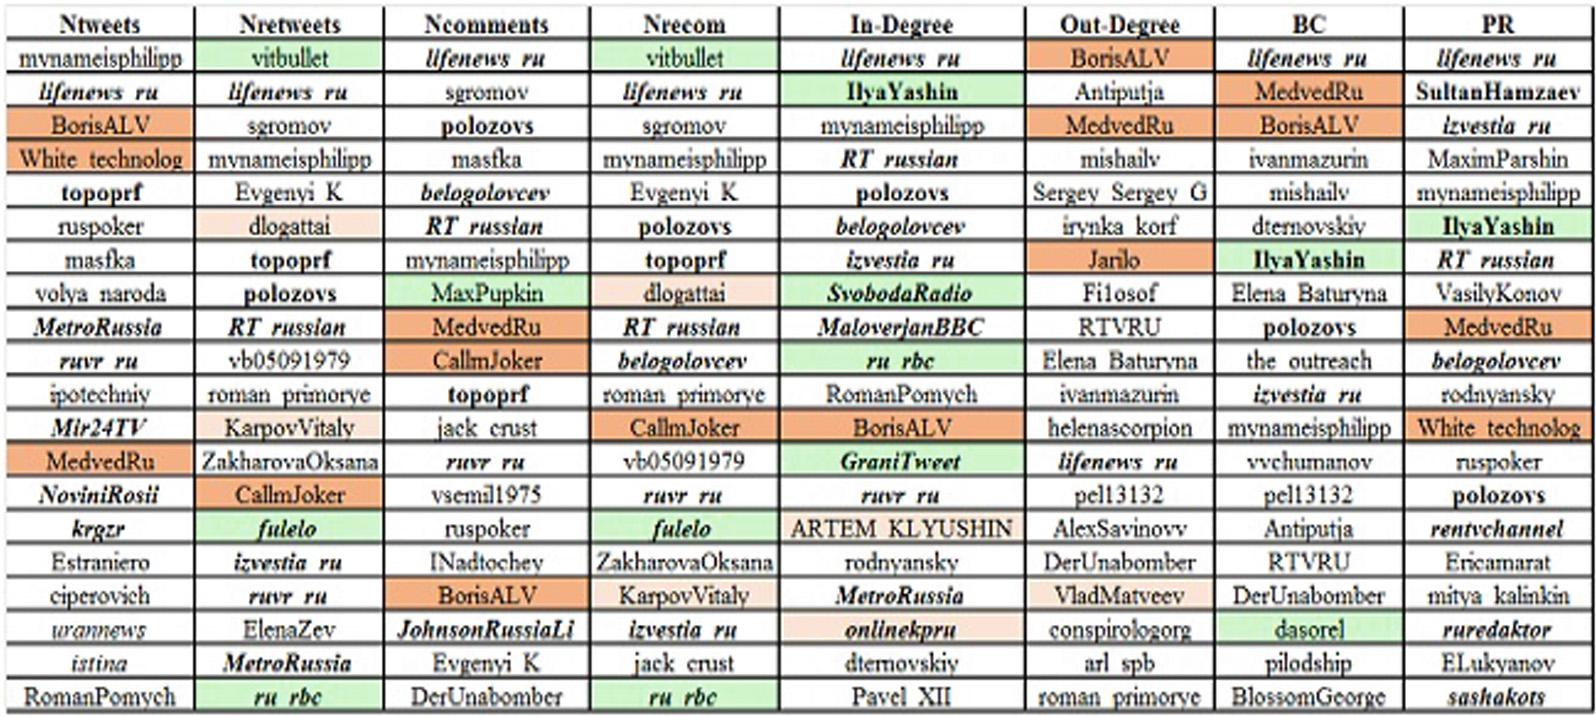
\includegraphics[scale=1.0]{topUsersRussia}
	}
	\caption{Institutional belonging and pro/contra-migrant positioning of top users in Russia.}\label{fig:topUsersRussia}
\end{figure} 

\begin{figure}[ht]
	\centerfloat{
		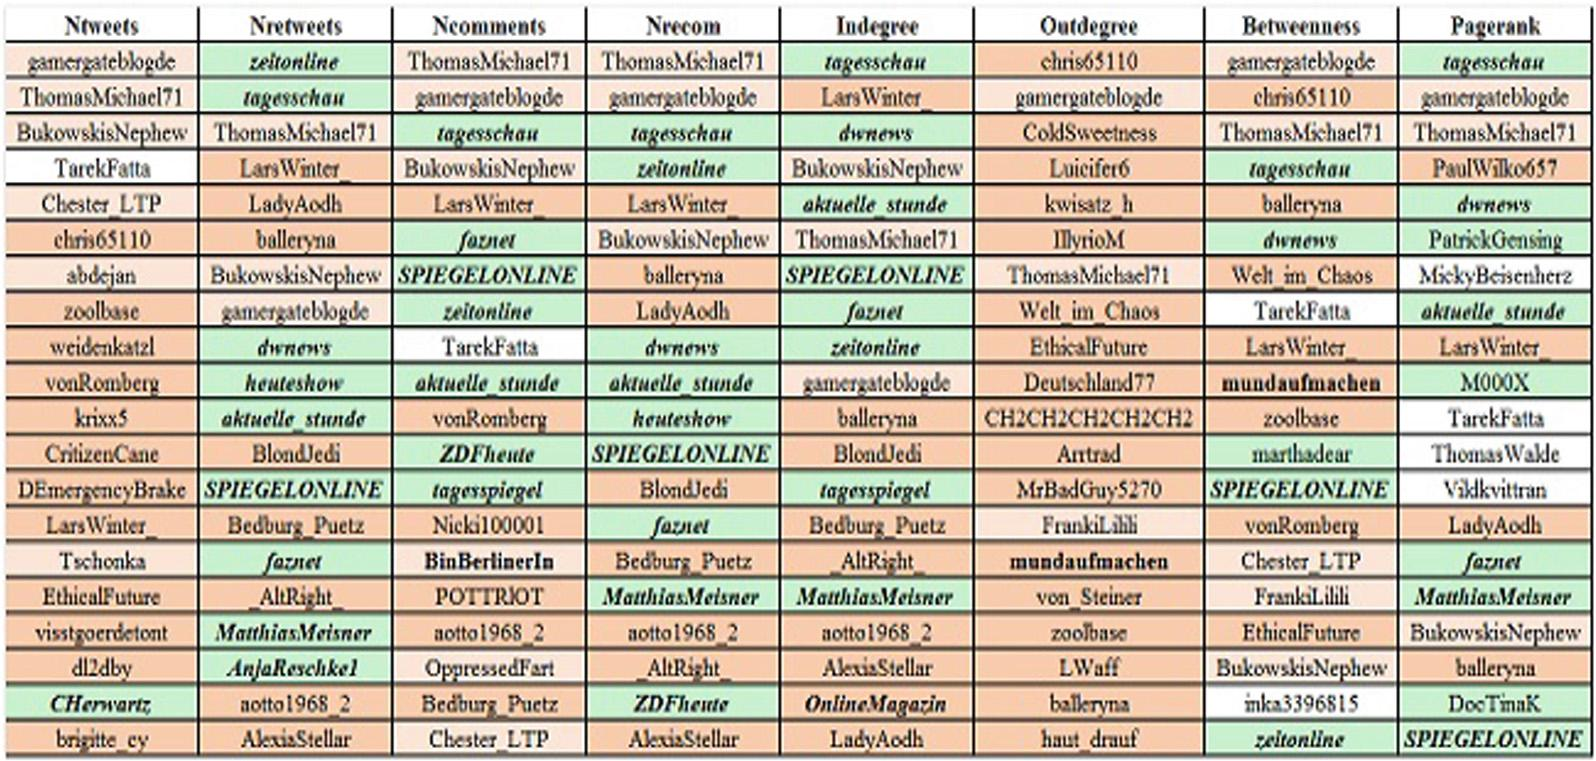
\includegraphics[scale=1.0]{topUsersGermany}
	}
	\legend{
		Regular -- ‘ordinary user’ \\
		Bold -- institutional user/representative \\
		Bold italic -- media account/journalist \\
		Italic -- ‘Twitter media’ \\
		Green -- strong/institutional support of migrants (absent from picture)\\
		Light green -- weak support of migrants \\
		White -- neutral user \\
		Light orange -- weak anti-migrant attitude \\
		Orange -- strong anti-migrant attitude/nationalist account.
	}
	\caption{Institutional belonging and pro/contra-migrant positioning of top users in Germany.}\label{fig:topUsersGermany}
\end{figure} 

\subsubsection{5. Results}

\paragraph{RQ1. Number of Tweets and Discussion Centers.} For both countries, the more users post, the more likely they become both ‘marketing’ (by \(N_{retweets}\) and \(N_{comments}\)) and ‘deliberative’ (by betweenness and pagerank) influencers, despite the difference in the size of datasets. The correlations remain in place for all the metrics for full and active-user datasets, despite the fact that elimination of ‘the crowd’ significantly drops outdegree for the Russian discussion and high values for \(N_{comments}\) and betweenness centrality for Germany. All in all, strength of the correlations remains comparable for all four of our datasets (though higher for Germany for the two aforementioned metrics), which might be telling of the nature of \textit{ad hoc} discussions on Twitter, but can also support the idea of the mediating role of \(N_{tweets}\); this needs further exploration.

But if we look closer at correlation values, we will see that outdegree correlates more weakly with \(N_{tweets}\) than other metrics throughout our data; this might mean that tweeting a lot does not provide for necessarily becoming commented or retweeted; the value is never higher than 0,418, and thus, the correlation is weak enough. Also, only in the German case, \(N_{retweets}\) matters for getting higher betweenness and pagerank, while in Russia their correlation is much weaker. But what, instead, seems to be important for becoming an influencer is a user’s indegree, that is -- how many users have interacted with you. This parameter becomes more important for becoming an authoritative node than the number of tweets, retweets, or comments -- the metrics that many works stated as markers of influencers. For all four of our datasets, the strength of ties between indegree and pagerank is 0,804 or higher. That is, a successful strategy within an \textit{ad hoc} discussion might be not to comment many times or get into a long meaningful discussion but to make a bigger number of users comment on you, perhaps by commenting them as well. On the other hand, outdegree does not seem to matter much for both betweenness and pagerank; this brings us to the conclusion that attractive content (which makes users interact with it) may be more important within such discussions than user activity.

\paragraph{RQ2. Institutionalization of the Discussion.} In Figs.~\cref{fig:topUsersRussia} and~\cref{fig:topUsersGermany}, we have marked institutional users, including media, bold (media -- bold italic). In general, the picture is similar in both countries and may be described as ‘liberal media against individual nationalists’. What is similar (and striking) in both countries is the absence of the much-awaited national/regional authorities, as well as NGOs and human rights watchers. We cannot prove dominance of institutional accounts over ‘ordinary users’, unlike in previous research \cite{XuSangBlasiola}, as we find only two politicians and one account of Public Advisory Chamber among the Russian top users, and two NGO-like organizations in the German top user lists.

Also, we cannot prove absence of nationalists as top users: in both countries, they are not only present but demonstrate blooming activity, and if in Russia they are most active in commenting, in Germany they lead both tweeting and commenting activities, all of them being non-institutionalized.

We call the picture similar, despite that, from Figs.~\cref{fig:topUsersRussia} and~\cref{fig:topUsersGermany}, the German discussion seems highly radicalized and the Russian one shows a lot of neutral users. But this may be explained by two factors. First, Biryuliovo happened over three years ago, and assessment of the accounts of top users does not bring over a lot of anti-migrant posts; this has cast its impact upon our allocation of users as neutral or biased. But we need to state that we have discovered a dominant mood among Russian ‘ordinary people’ which may be described as ‘angry patriotism’: today, such users (over a dozen in the Russian top lists) express ‘patriotic’ views like supporting Donbass population or tweeting on national pride (e.g. on leading industries like aviation, military equipment etc.) but at the same demonize the current country’s leaders as corrupt and ineffective. Thus, these users are highly politicized, no less than the German users; it is just not always possible to deduce their attitude from the tweets of the discussion (especially if they retweeted other accounts) and today’s tweets. Second, some media accounts in the Russian list (like lifenews\_ru, izvestia\_ru, or RT\_russian) were marked neutral, as we could not find direct proof of their anti-migrant bias, but their overall tone is pro-establishment, and thus their position fluctuates from supporting the state views on open visa regime for Central Asian post-Soviet ethnicities to populism of attaching social and cultural threats to their communities. Having said this, we can consider the situation similar indeed in both cases, as it is highly polarized, full of political criticism, and intolerant.

\paragraph{RQ3. The Place of Media in the Discussions.} Media, indeed, occupy a significant place in the discussion and represent a variety of political views and positions. Unlike on Russian Facebook, in this discussion both pro-establishment and highly oppositional media (ru\_rbc, GraniTweet), as well as foreign liberal media and journalists (MaloverjanBBC, fulelo, SvobodaRadio) are present, and the liberal-oppositional media show their efficacy, as they become retweeted and commented by many people without tweeting a lot. In Germany, it is mainstream media, and mostly newspapers, that also become influencers without posting a lot; they get retweeted and commented in general and by a lot of users in particular, and gain high pageranks. But even if so, media do not outperform nationalist users, and they do not get high betweenness centrality, which means that they do not play the role of ‘information mini-hubs’ as the basic nodes of the online public sphere. They remain authoritative (especially in Germany), but the niche of ‘deliberative connectors’ remains free and is occupied by the most polarized users. Thus, the ‘opinion crossroads’ may be there in terms of representation of views within the whole discussion but it is still a question whether the opposing views actually have a chance to meet.

\paragraph{RQ4. Neutrality of Top Users.} As already stated above, neutrality of users cannot be proven, especially in case of Germany. In Russia, general negative politicization of the audience goes along with nationalist and pro-nationalist views, and in Germany the discussion after a major public harassment is shaped not by the forces countering intolerance but by openly anti-migrant discussants; in both cases, it is individuals that polarize the discourse against re-settlers and media that counter this -- even if due to different reasons. Thus, for most of the German media, supporting immigrants is a non-valent issue, and expressing an alternative position would amount to a scandal. In Russia, the division between pro-establishment and oppositional media is also true for the migration issues, and thus liberal-oppositional media support their political standing by expressing pro-migrant views.

\subsubsection{6. Conclusion}

We have looked at two \textit{ad hoc} discussions on violent inter-ethnic conflicts, namely the Biryuliovo bashings in 2013 and mass harassment in Cologne in 2016, to see whether in such discussions user activity leads to higher positions within the discussion network and higher connectivity. Along with this, we assessed the substantial features of top users, such as their institutional status and opinion positioning.

Despite the differences in samples, we have managed to show that comparing influencers is possible, and there are patterns in the structure of influencing that are similar. The main methodological finding is that, in both discussions, the number of users involved mattered more for becoming an influencer (by BC and PRC) than the number of actual tweets, retweets, or comments received by a user.

Though direct comparisons were not always possible by our methodology, we have found more similarities in the two cases than we had expected. Thus, in both countries, the situation may be described as opposition ‘liberal media vs. nationalist users’, and the absence of both authorities and NGOs is striking. Media do become influencers, but in terms of authority (or ‘marketing’ approach) rather than in deliberative terms, as they do not get high betweenness centrality and thus may have difficulties in performing the roles of shapers of information flows. In both countries, the discussion was highly opinionated and emotionally heated even within several weeks after the events, and seemingly higher neutrality of the Russian users was compensated by their overall politicization and rebuttal modus.

Thus, as to the question of whether and how ‘opinion crossroads’ are forming, there is evidence that, in general, left-right or in-system/oppositional views are well represented by media within the discussions. But virtual absence of pro-migrant institutions and opposition of liberal media to pro-nationalist ‘ordinary users’ shows that, in both countries, the discussion is far from being balanced, rational, and inclusive.

\subsection{Public Opinion Dynamics in Online Discussions: Cumulative Commenting and Micro-level Spirals of Silence}\label{subsec:ch2/sec4/sub5}

\subsubsection{1. Introduction}

Social media have become a place where the bulk of grassroots political discussion takes place. Social networking sites, online platforms, and messengers have become a focus of scholarly attention in their relation to public opinion formation and spread, which, in its turn, directly affects the quality of offline democratic deliberation.

The models that described opinion formation in the era of traditional media have been applied to online discussions, with varying degree of proof and support. Thus, the idea of opinion leaders \cite{KatzLazarsfeld} has been re-interpreted to describe the practices of influencers \cite{Gillin,BakshyHofmanMason,BodrunovaLitvinenkoBlekanov2017}, and the older idea of echo chambers \cite{Key} has transformed into filter bubbles \cite{Bruns2019}.

Along with this, today’s public spheres are, in general, described as dissonant \cite{Pfetsch} and discontinued \cite{SmoliarovaBodrunovaBlekanov2020}. The dynamics of formation of dominant opinions have been conceptualized in several theoretical models, among them, most famously, in the idea of spiral of silence \cite{NoelleNeuman1974}. In this conceptualization, under pressure of fear to be excluded, supporters of one candidate become gradually silenced by the supporters of the other one, and the latter are capable of doing this just by expressing their opinion more massively.

However, when applied to the dissonant and disruptive online discussions of today where cumulation of support is often accompanied by communicative aggression \cite{Sidorov,BodrunovaLitvinenkoBlekanov2021}, Noelle-Neumann’s concept and similar conceptualizations needs to be reconsidered and re-tested. This is especially because there is growing evidence that online discussions are the place where silent majority flourishes \cite{MustafarajFinnWhitlock,ChenLiYao,McKeeverMcKeeverHolton,MaiShanBai}.

Today, instead of dialogue and polylogue in the forms of opinion exchange, we witness cumulative modes of discussion prevail \cite{BodrunovaLitvinenkoBlekanov2021}. To re-conceptualize the ways public communication exists and develops in online milieus, we suggest the idea of \textit{cumulative deliberation} on which we elaborate below (see Sect. 2). Our previous works, as well as many works before ours, have shown that cumulation may be regarded as a universal mechanism of public opinion growth and polarization \cite{BodrunovaBlekanovSmoliarova}. E.g., in the form of echo chambering, it works on many levels in globalized discussions, such as language, hashtagging, and sentiment \cite{BodrunovaBlekanovKukarkinCH}. We have also demonstrated that, on Russian oppositional YouTube, users hardly form what might be called ‘a discussion’; they, rather, express themselves \textit{urbi et orbi} without entering any dialogue with particular users, despite their high polarization in political terms and an extremely high level of aggressive and hate speech discovered \cite{BodrunovaLitvinenkoBlekanov2021}.

The current paper further fosters the idea of discovering patterns of cumulative deliberation in oppositional discourse and, this time, uses a year-long dataset from Belarusian oppositional YouTube of 2018. We have collected comments left by users under the videos of six salient Bealrusian oppositional accounts (one of which, Nexta, has become world-renowned during the Belarusian protest of 2020). We have identified users who linked these accounts by posing to at least five of them, and have analysed this core of commenting for the features important for the deliberative process, namely orientation to dialogue \cite{Ksiazek}, aggression \cite{BodrunovaLitvinenkoBlekanov2021,KsiazekPeerZivic}, and political criticism. In the latter we have taken in mind the difference between uncritical, policy-critical, and leadership critical publics, as it was suggested and explained for authoritarian societies \cite{Toepfl}.

In particular, we focus on two research questions. First, we ask whether (and how exactly) the deliberative features mentioned above accumulate in the discussion and affect its dynamics in the core of the discussion (which is, in the Belarusian case, the cross-commenter conglomerate) on various time spans. Second, we look at whether the deliberative feature of the discussion core affect the bulk of the discussion. This paper is only a trial that shows the necessity of further exploration of cumulative patterns of online discussions and points out to possible bigger cumulative effects that deserve exploration and explanation.

The remainder of the paper is organized as follows. Section 2 elaborates on cumulative deliberation as a concept and suggests how dynamics of the discussions might be affected by cumulative patterns of opinion formation. Section 3 poses the research questions. Section 4 describes sampling, data collection, dataset limitations, and methods of data assessment. Section 5 provides the results; Sect. 6 discusses them and concludes the paper.

\subsubsection{2. Cumulative Foundations and Deliberative Features of Online Opinion Formation}

\paragraph{2.1 Cumulative Patterns in Online Opinion Formation}
As already stated above, the idea of cumulation as a basic principle of how online public opinion forms has come from two streams of literature.

\paragraph{Cumulative Effects in Online Opinion Formation.} The first one focuses upon patterns	of winning the public debate -- that is, majority/minority formation in public opinion and electoral research. In political sociology, the works that have demonstrated that people may change opinion just knowing or supposing what others might think have been numerous \cite{NowakSzamrejLatane}, and they have posed a question of whether opinion change is a result of persuasive external arguments, including mediated ones.

However, despite their evident high impact upon the rational choice debate, relatively few important works linked individual/public opinion shifts to communication and deliberation patterns on aggregated levels. Well-known are, e.g., the works on ‘spiral of silence’ by Elizabeth Noelle-Neumann \cite{NoelleNeuman1974} or Latané’s social impact theory that emerged, i.a., from studying interaction patterns \cite{NowakSzamrejLatane,Latane}. But it was not before the advent of social media that the scholars have received a chance to study the multi-level communicative interactions.

There is one significant factor that distinguishes the pre-Internet era from today’s communication. In online communication, the iceberg of what could previously remain an oral utterance exchange and disappear forever after being pronounced, remains written and accessible by the newcomers who join the communicative milieu later in time. Potentially, this casts impact upon the newcomers and their personal, seconds-long opinion formation, in accordance with the social impact theory; this remains highly understudied. At the same time, there is a substantially bigger corpus of works upon various discussion-level effects of opinion cumulation, such as echo chambering and filter bubbles studies or research on influencers who become such by cumulation of user support. (Of these studies, we will focus on user comments studies -- see below).

Thus, cumulative effects in communication have long been demanding generalization
and systematization -- or at least a proper acknowledgement of the role of cumulation in
opinion formation online.

\paragraph{Dissonant Public Spheres: Getting Rid of Excessive Normativity.} The second stream of literature is that on public sphere as a normative space of (arguably) consensusoriented discussion of conflictual issues in public domain, as well as on deliberation as a special form of public communication, an imagined round-table process of collection and adjustment of individual, group, and institutionalized opinions that leads to decision on a given issue. For several decades, public sphere studies have almost exclusively, either adhering or critically, oriented to the works by Juergen Habermas.

The Habermasian view on deliberation is known for its high normativity, as communicative actions need to be rational, consensus-oriented, and civil in order to count for public decision-making. Despite the overwhelming amount of academic criticism from both left and right parts of the political spectrum, as well as the shifts in Habermas’s own conceptualization of public sphere and deliberation, the normative notion of orientation to consensus (or to struggle, in the leftist view \cite{Mouffe}) and high \textit{deliberative quality} of public communication was not challenged.

Again, it was not before the advent of blogs and social networking sites that the scholars questioned the belief that people come into a discussion either ‘to agree or to argue’ \cite{YardiBoyd} -- that is, with a certain deliberative goal. Today, this notion has been shaken by description of online public spheres as dissonant -- that is, not aiming to consonance and consensus; public spheres where myriads of actors express themselves simultaneously \cite{Pfetsch}. There are also works that describe public spheres as discontinued, whose actors constantly change and re-aggregate \cite{SmoliarovaBodrunovaBlekanov2020}, and, in general, disrupted \cite{BennettPfetsch}.

Moreover, recent research suggests that users might participate in dialogical forms of communication much more rarely than deliberation theory suggests \cite{BodrunovaLitvinenkoBlekanov2021}, and that their motivation is neither to agree nor to argue in order to come to a conclusion, but more to express themselves, solidarize with an earlier opinion or negate it without having in mind any longer-term effects. Yet, even such communicative activity, ‘irrelevant, aggressive, and stupid’ \cite[p.~659]{SchultesDornerLehner}, seemingly aimless in deliberative terms and dismissed as slacktivism \cite{Morozov} and ‘sofa warrior’ behavior, acquires importance if seen from the cumulative-effects viewpoint.

The plea for finding new grounds for assessment of public spheres influenced by massive micro-level communication, united with the view upon cumulation as an overarching pattern of how opinion aggregates and dissipates online, has led us to the concept of \textit{cumulative deliberation}. This concept is, in essence, an alternative vision on public deliberation that covers by one umbrella many cumulative effects scattered around academic works on older and newer media and opinion formation via them. Cumulative deliberation allows for a closer-to-reality look at how people talk online, as it lets avoid the excessive normativity and merit the smallest forms of online user activity: each individual comment, like, share, or mention matters for cumulative deliberation. It also aims at discovering patterns of opinion aggregation on various levels and explaining/predicting critical thresholds in cumulative communication. And the patterns of opinion cumulation, not only user intentions, should be subjected to critical assessment within the democratic perspective of public communication.

\paragraph{2.2 User Comments on YouTube and Other Social Media: The Issue of Deliberative Quality of Communicative Micro-action}

Thus, user commenting seen as deliberative activity may be put into the cumulative deliberation perspective -- that is, cumulative patterns and their effects in user commenting need to be detected and assessed, without putting the blame to users for not being rational or purposeful. Previous research shows that users’ comment ‘exchange is socially and not deliberatively motivated’, and, in reading comments, ‘entertainment dimension -- a dimension that is not usually considered to be linked to deliberation processes -- is the more stable one’ \cite[p.~798]{SpringerEngelmannPfaffinger}. This points out to the necessity for the academe to move towards accepting these motivations as normal and assessing the cumulative effects of such online posting.

Close enough to this notion, computational social scientists have tried to detect statistical effects in comment threads and discussion graph structure, such as various types of distributions like lognormal \cite{GomezKappenKaltenbrunner}, negative binomial \cite{TsagkiasWeerkampDeRijke}, Zipf’s law \cite{KumarMahdianMcGlohon}, or power law \cite{BodrunovaBlekanov}. However, cumulative effects may be of a more nuanced nature, as they combine statistical features of communication flows and contents of user utterances (for a short review on early works that include content features into statistical modelling of commenting dynamics, see \cite{WangYeHuberman}). Even successful modelling of discussion growth \cite{WangYeHuberman} often sees comments as discreet items, not cumulative conglomerates, and fails to encompass deliberative features of comments (sometimes focusing on one selected). On the other hand, communication scholars who focus on deliberative quality of commenting \cite{Rowe} are less attentive to various formal levels on which cumulation might shape the discussion, as well as to statistical features of discussions linked to platform affordances and human capacities that define posting and reading.

In our current research, we do not aim at creating overarching models of user commenting; we just want to demonstrate easily discoverable impact of deliberative features of user posts upon various structural levels and temporal fragments of online discussions. In previous studies, several user-dependent features of comments and their deliberative potential have been discussed. In a more systematic view, assessment of democratic qual- ity of deliberation online moves from evaluating the constellation of major institutional discussants to single user and features of their statements.

\paragraph{Orientation to Dialogue.} Addressing the other is an inevitable pre-requisite for any sort of dialogue, public or private. Interactivity has been conceptualized as capable of ‘contribut[ing] to shaping a democratically valuable and vivid interpersonal discourse on topics of public interest’ \cite[p.~1112]{ZiegeleBreinerQuiring}; see also \cite{BoczkowskiMitchelstein,Freelon,RuizDomingoMico}. However, user comments do not necessarily have this feature. Thus, an important division has been introduced between user-to-content (e.g., news video) and user-to-user orientation in commenting \cite{KsiazekPeerZivic}, and user-to-content comments, as a rule, do not involve other users to interaction.

While we praise this important distinction, we prefer to see formal interactivity (often marked by user mentions) as just a part of wider orientation to dialogue. Thus, our earlier study \cite{BodrunovaLitvinenkoBlekanov2021} shows that, on Russian-speaking YouTube, ‘discussion’ in the form of dia- logue hardly takes place at all, despite the political topicality of the assessed videos, and formal and substantial markers of dialogue may not correspond. E.g., even when users formally reply to other users’ comments, they construct the phrases the way that does not invite their correspondents to answer; they just solidarize with the expressed opinion or share their own experience that, in most cases, supports the view in the primary post. Or, vice versa, a comment may be openly dialogical in substance (interrogative, sarcastic, or denialist) without any formal interactivity features. In normative view, dialogue features should oppose.

\paragraph{Aggression.} When a dialogue does take place, it may easily take an anti-normative direction, as users attach each other aggressively, rather than interact in civil manner. Studies of user sentiment, emotions, affect, and aggression in social media content are overwhelming in number. Of emotional substance of comments, various types of aggressive speech are the sharpest; this, i.a., includes hate speech, obscene and tabooed lexicons, politically motivated offence, calls for violence, cyberbullying, humiliation, and harsh shaming. However, we have demonstrated \cite{BodrunovaLitvinenkoBlekanov2021,BodrunovaNigmatullinaBlekanov} that communicative aggression may play constructive roles in online discussions, such as influencing its dynamics and performing individual- and group-level psychological functions.

Today, surprisingly few works focus on how aggressive and emotional speech relates to opinion aggregation and fueling discussions. This is especially true for languages like Russian and Belarusian where obscene lexicon has grown into a highly developed sub-language.

\paragraph{Criticism.} Aggression needs to be distinguished from criticism, another pragmatic dimension of user speech. Critical assessment of reality has for centuries been acknowledged as a pre-requisite for substantial debate on nearly any issue. Political criticism may be directed to individual/group ideological opponents, as well as to the state, public bodies, persons, and policies. Recently, three types of publics have been defined for authoritarian public spheres, based on what is subjected to criticism \cite{Toepfl}, namely uncritical, policy-critical, and leadership-critical publics. Criticism to policies is expected to be milder, more discussion-oriented, and perhaps a bit more toothless, as it follows from the paper. Criticism towards the authorities brings more dangers to the speaker and, thus, demands passing a certain psychological threshold. This might imply that leadership-critical users could use aggressive speech and be less willing to take part in meaningful discussion. Both critical stances, however, may foster cumulative effects in discussions, as earlier critical comments may help diminish participation thresholds for users who comment later, and thus create avalanche effects.

Taken together, these three deliberative features may work on various levels of online discussion architectonics, from single comments to platform-based publics. We will look at their potential to foster cumulative effects in online communication on Belarusian YouTube.

\subsubsection{3. Research Questions}
Having said that, we have formulated the research questions for our study.

\paragraph{RQ1. Are the three deliberative features relate to each other in the discussion, and how?}

\paragraph{RQ2. Do the three deliberative features influence the discussion dynamics, and on what levels and time spans?}

\paragraph{RQ3. Are there any distinctive patterns of cumulative deliberation that we can point to, and on what levels and time spans?}

We do not pose any exact hypotheses, as our study is exploratory; below, we will summarize our findings according to the RQs stated above.

\subsubsection{4. Data Collection and Methods}

\paragraph{4.1 Case Description: Belarusian Oppositional YouTube}

To address the research questions, we have used the dataset of comments published within the year of 2018 to six YouTube accounts from Belarus, all of them politically oppositional, most salient on Belarusian political YouTube in 2018--2019.

This choice is explainable in many respects. First, Belarus remains one of most understudied media landscapes of Europe; as a recognized autocracy, it represents a case for analysis of authoritarian public sphere. Second, the dataset is not hashtag-based, which allows for avoiding the dissipative and affective effects \cite{Papacharissi} in how it develops; the dataset represents a ‘chronic’ discourse on the oppositional YouTube. Its oppositional orientation allows for comparing the results with our earlier work on Russia \cite{BodrunovaLitvinenkoBlekanov2021}; the pre-set political standing of channels sets the conditions for potentially conflictual and polarized opinion exchange. Al the same time, the volume of discussion is by an order of magnitude smaller than in Russia and the most studied Western countries, due to lower levels of YouTube consumption and smaller populace in general; thus, a year-long dataset remains feasible for both automated and manual research. In this respect, Belarusian YouTube is sort of an ‘ideal gas’ of studying online political communication in autocracies. To this, we add that, to avoid geographical echo chambering, we have focused not only on the accounts based in Minsk but also on those produced in other Belarusian regions. The accounts are Belsat (Belarusian oppositional satellite TV channel sponsored from abroad), Nexta (by 2021, a world-famous Belarusian blogger and protest facilitator), Garantiy NET (‘No guarantee’, Gomel; by 2021, the videos of 2018 are deleted), Narodny Reporter (‘Popular reporter’, Brest region), The Belarusian Experimental Field (positioned as all-Belarusian), and Rudabelskaya pakazuha (‘Window dressing in Rudabelka’, Gomel region).

It is worth mentioning that, in 2020, Belarus has lived through a months-long political protest unprecedented in the newest Belarusian history. The data of a year and a half before the protests erupted demonstrate the mood of Belarusians and are relatively highly politicized.

\paragraph{4.2 Data Collection and the Dataset}

YouTube crawling was performed by the web crawler created and patented by our research group \cite{BlekanovSergeevMartynenko}. The overall number of user comments in the dataset is 120,412 posted by 3000+ users.

\paragraph{4.3 Research Procedures and Methods Used}

The logic of our research demanded several steps of working upon the dataset.

\paragraph{Defining the Discussion Core.} After preliminary studying of comment structure and their appearance on actual YouTube pages, we have divided the dataset into the core and periphery. The core users were those who performed an important deliberative function of cross-account commenting, thus transforming the accounts and the discussion into one discursive field. Reconstructing the web graph of the discussion by the YifanHu Gephi algorithm, we have identified users who posted in at least five of six accounts (76 users with 8,610 comments). Answering the RQs was linked to both the discussion core itself and to relations between the core and the periphery of the discussion.

\paragraph{Forming Sub-Datasets.} We have identified the levels on which we search for cumulative patterns. We have used seven levels/time spans formed from the bulk data. The logic of it is to ‘zoom in’ from the whole discussion to the level of one particular day (step-by-step via other time spans), one video, and one user. The sub-datasets used for this paper include the following (see Table~\cref{tab:projectSubdatasets}).

\begin{table}[ht]%
	\centering
	\caption{Sub-datasets of the project.}%
	\label{tab:projectSubdatasets}% label всегда желательно идти после caption
	\begin{adjustbox}{width=1\textwidth}
		\small
		\begin{tabular}{ l  l  l  l  l }% Вертикальные полосы не используются принципиально, как и лишние горизонтальные (допускается по ГОСТ 2.105 пункт 4.4.5) % @{} позволяет прижиматься к краям
			\toprule
			\# & Time span & \makecell[l]{Unit of analysis\\/ Granger test increment} & Type of data & N of comments \\
			\hline
			(1) & Year & Any & \makecell[l]{The whole discussion\\bulk (used to detect\\the core and form\\other datasets)} & 120,412 \\
			(2) & Year & Week & \makecell[l]{The whole discussio\\core} & 8,610 \\
			(3) &  \makecell[l]{5 weeks, February 26\\to April 1} & 24 h & The most rapidly growing discussion segment around a key event &  \makecell[l]{(3a) 1,164 -- core vs\\(3b) 17,222 -- bulk} \\
			(4) &  \makecell[l]{Week, March 26\\to April 1} & 6 h &  \makecell[l]{The most commented\\week around a key\\event} & 287 \\
			(5) & Day, March 26 & 1 h &  \makecell[l]{The day next to the\\key event} &  \makecell[l]{(5a) 113 -- core vs. (5b) 1,269 -- bulk} \\
			(6) & Year & Year &  \makecell[l]{Comment\\conglomerates by each\\cross-commenter} & 8,610 \\
			(7) & Year & Year &  \makecell[l]{Comments under a\\particular video of\\March 25} & 127 \\
			\bottomrule
			\multicolumn{5}{@{}p{\textwidth}}{%
				\hspace*{2.5em}% абзацный отступ - требование ГОСТ 2.105
				\textit{Note}. The sub-datasets (3a), (4), (5a) are formed out of the sub-dataset (2) and, thus, were coded within the coding process for the sub-dataset (2).
			}\\
		\end{tabular}%
	\end{adjustbox}
\end{table}

Zooming in was performed after detecting the most actively growing segment of the year-long discussion. This segment was 5 weeks from February 26 to April 1, 2018, structured around an event of high importance to the opposition, namely the celebration of 100 years of the so-called 1918 Belarusian Republic (March 25, most active commenting taking part on March 26).

\paragraph{Coding Deliberative Features of Comments.} The contents of the sub-datasets (2) including (3a), (4), and (5a), as well as (6) and (7), were coded for the three deliberative features described above, that is, orientation to dialogue (‘dialogue’ from now on), aggression, and criticism.

For the latter, we have introduced additional variables after preliminary reading of the data and following Toepfl’s argument \cite{Toepfl}. Thus, three more coding variables were added: criticism towards authorities/security services (corresponding to ‘leadership-critical public’), and self-criticism. We have discovered this phenomenon of Belarusians criticizing themselves and self-blaming for the political situation in the country and have coded this as a separate variable. Thus, ‘criticism’ was coded as comprising the three types of critique found in the comments.

The coding was performed by two coders (Cohen’s kappa = 0,81), both speaking native Russian and Belarusian, as the discussion was bilingual.

\paragraph{Testing the Dependencies.} For testing the inter-relation between the variables, descriptive statistics (Cramer’s \(V\)) were used. For demonstration of discursive divergence of the cross-commenters, k-means clustering with silhouette quality metric was applied. For assessment of the possible impact of the deliberative features to discussion dynamics, Granger testing was used.

\subsubsection{5. Results}

\paragraph{RQ1.} \textit{Inter-relation between the deliberative features and their impact to discussion structure.} After we have coded the data, it became evident that dialogue, aggression, and criticism were inter-related in our data in specific ways that might relate to cumulation of support or criticism during the discussion.

From the first correlation tests we have seen that, counter-intuitively, aggression is linked not to criticism but to dialogue, and, moreover, this inter-relation intensifies on the most intense commented days (see Tables~\cref{tab:commentInterRelationYearly} and~\cref{tab:commentInterRelationWeekly} for year-long and day-long spans, respectively). Dialogue and aggression correlate strong enough, while none of criticism types correlates with dialogue or aggression, and criticism to power and self.

\begin{table}[ht]%
	\centering
	\caption{Inter-relation between deliberative features in the comments of cross-commenters on the year-long span (Cramer’s V, N = 8,610).}%
	\label{tab:commentInterRelationYearly}% label всегда желательно идти после caption
	\begin{adjustbox}{width=1\textwidth}
		\small
		\begin{tabular}{ l  l  l  l  l  l  l }% Вертикальные полосы не используются принципиально, как и лишние горизонтальные (допускается по ГОСТ 2.105 пункт 4.4.5) % @{} позволяет прижиматься к краям
			\toprule
			Deliberative feature & Dialogue & Aggresion & Criticism & Criticism power & Criticism policy & Criticism self \\
			\hline
			Dialogue & 1.000 & & & & & \\
			Aggresion & 0.289*** & 1.000 & & & & \\
			Criticism & \(-0.177\)*** & \(-0.074\)*** & 1.000 & & & \\
			CriticismPower & \(-0.151\) & \(-0.014\) & n/a & 1.000 & & \\
			CriticismPolicy & \(-0.048\)*** & \(-0.052\)*** & n/a & \(-0.107\)* & 1.000 & \\
			CriticismSelf & \(-0.043\)*** & \(-0.076\)*** & n/a & \(-0.156\)*** & \(-0.054\)*** & 1.000 \\
			\bottomrule
		\end{tabular}%
	\end{adjustbox}
\end{table}

\begin{table}[ht]%
	\centering
	\caption{Inter-relationbetweendeliberativefeaturesinthecommentsofcross-commentersona weekly span, March 26 to April 1 (Cramer’s \(V\), \(N = 287\))*.}%
	\label{tab:commentInterRelationWeekly}% label всегда желательно идти после caption
	\begin{adjustbox}{width=1\textwidth}
		\small
		\begin{tabular}{ l  l  l  l  l  l }% Вертикальные полосы не используются принципиально, как и лишние горизонтальные (допускается по ГОСТ 2.105 пункт 4.4.5) % @{} позволяет прижиматься к краям
			\toprule
			Deliberative feature & Dialogue & Aggresion & Criticism & Criticism power & Criticism self \\
			\hline
			Dialogue & 1.000 & & & & \\
			Aggresion & 0.470*** & 1.000 & & & \\
			Criticism & \(-0.347\)*** & \(-0.243\)*** & 1.000 & & \\
			CriticismPower & \(-0.299\)*** & \(-0.205\) & n/a & 1.000 & \\
			CriticismSelf & \(-0.153\)* & \(-0.095\) & n/a & \(-0.143\)* & 1.000 \\
			\bottomrule
			\multicolumn{6}{@{}p{\textwidth}}{%
				\hspace*{2.5em}% абзацный отступ - требование ГОСТ 2.105
				*\textit{Note}. The correlations between criticism to policy and other variables was not tested due to scarcity of data.
			}\\
		\end{tabular}%
	\end{adjustbox}
\end{table}

Based on this finding and on the insights from the coding process, we have tested whether the discovered correlations matter on the user level -- that is, whether there are distinct discursive clusters that would diverge, e.g., the ‘dialogical and aggressive’ users and critical users. For this, we have used \(k\)-means clustering and silhouette as a quality metric (see earlier accounts on this method used for social media data in \cite{BodrunovaBlekanovKukarkin2018}).

Indeed, we have discovered that two clusters form well enough (\(S > 0,6\); see Fig.~\cref{fig:twoClusterDivergence}); however, the two clusters diverged only on aggression \((p = 0.000)\) and dialogue \((p = 0.001)\), not on criticism \((p = 0.3)\). The best clustering option (of over two dozen probed, from 2 to 5 clusters, from 3 to 5 variables) is presented on Fig.~\cref{fig:threeClusterDivergence}, it has three clusters and is based on the three initial variables (for all variables, \(p < 0.0002\)). On Fig.~\cref{fig:threeClusterDivergence}, the aggressive-dialogical Cluster 3 is formed by 4 users only, with the rest of the users distributing nearly equally between two ‘calm’ clusters with varying level of criticism. However, if we use another sorting option (with observations taken as fixed intervals), their number grows to 15.

\begin{figure}[ht]
	\centerfloat{
		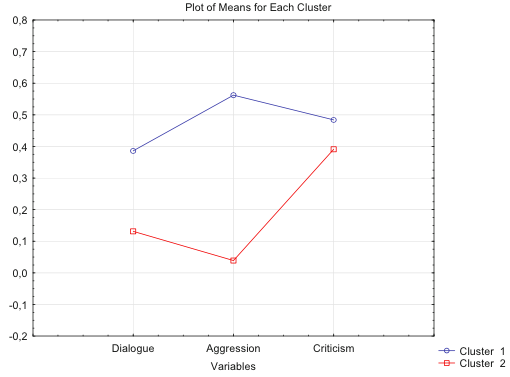
\includegraphics[scale=1.0]{twoClusterDivergence}
	}
	\caption{Plot of means for two-cluster divergence of cross-commenters.}\label{fig:twoClusterDivergence}
\end{figure} 

\begin{figure}[ht]
	\centerfloat{
		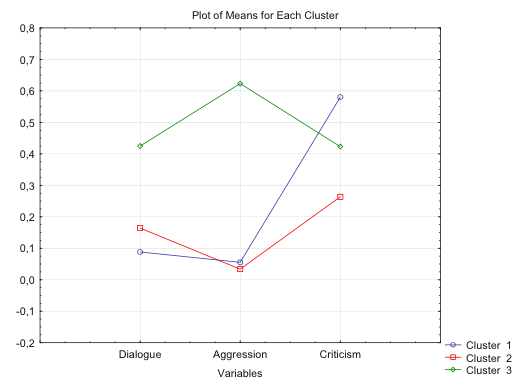
\includegraphics[scale=1.0]{threeClusterDivergence}
	}
	\caption{Plot of means for three-cluster divergence of cross-commenters.}\label{fig:threeClusterDivergence}
\end{figure} 

This supports what we have seen during coding. There are two modes used by cross- commenters of our dataset. Mostly, users self-express ‘urbi et orbi’ or, more rarely, address their comments to the authors of the discussed videos. There were nine users among 76 who never addressed anyone and just commented by expressing themselves; for 42 of 76 users (55\%), dialogue-oriented comments were fewer than 10\%. Such users seem to form a personal ‘opinion bubble’ which they stretch across the YouTube channels they comment in. The dialogue appears to ‘belong’ to other users that enter aggressive interrogations with other users (whom they often dismiss as trolls), and these micro-skirmishes evolve into microscopic ‘spirals of silencing’ one of the opponents.

Another interesting, even if intuitively understandable, finding is that self-criticism is inversely proportional to criticism to authorities, as well as to policy criticism (despite the fact that all options could be coded for one comment). However, unlike criticism on the whole, self-criticism does not help users diverge. We have tested self-criticism in various combinations of variables for 2, 3, and 4 clusters, and self-criticism was never significant. Thus, this modus is spread all over the discussion core, but in small proportions which are not enough to influence individual user strategies; only 12 of 76 users (circa 16\%) have not expressed self-criticism in their comments.

\paragraph{RQ2.} \textit{Impact of the deliberative features to the discussion dynamics.} To assess whether the deliberative features cast impact upon the discussion dynamics, we have tested the relations between the overall number of posts and the number of posts with deliberative features for various time spans (see Table~\cref{tab:projectSubdatasets}). After our findings for the Russian YouTube of 2019 [11] where we have seen that aggression highly influences discussion dynamics, as well as vice versa, we expected this to be also true for the Belarusian YouTube.

However, of all the Granger tests we have conducted for weekly, daily, 6-h, and hourly spans, only two cases detected dependencies. Thus, by Granger tests, dynamics of self-criticism shaped the dynamics of the discussion core in 6-h increment, both for the overall number of posts (6.3*, \textit{p = 0.021}) and for the posts with self-critical ones excluded (5.64*, \textit{p = 0.03}). In its turn, criticism in the discussion core affects the number of comments in the whole dataset within one day (1-h increment). This may point out to a cumulative pattern of core-to-periphery influencing: when criticism in the core discussion grows or diminishes, intensity of the whole discussion changes accordingly. This, of course, needs more testing to detect stricter patterns of influence; however, for the discussion under scrutiny, we see that the macro-levels (yearly and monthly spans) are too loose in terms of number of posts to create meaningful patterns of cumulation, while, within hours, the discussion fluctuates depending on how critical it is.

Another interesting finding, perhaps, is that neither the overall number of comments casts impact upon the number of comments with distinct deliberative features, which is counter-intuitive. We think that this effect is related to the fact that the discussion is too loose in terms of number of posts in time. In non-dense discussions, each week and day start anew: what was said before, even immediately before, neither spurs nor slows down the pace of dispersed user commenting. This is also supported by how the number of comments in the core and the whole discussion inter-relate: their correlation is very high (R Pearson 0.880***), but Granger test does not show any mutual impact (which was expected, at least in terms of impact of the whole discussion upon its core).

This, combined with the knowledge of low orientation to dialogue, creates a picture of dispersed, self-expression-oriented, and non-deliberative \textit{cumulative commenting}. Despite formally present user-to-user comments, they do not involve users into opinion argumentation and (dis)agreement. What they do is perhaps lowering entry thresholds for those who would like to express their dissent towards authorities and the country.

\paragraph{RQ3.} \textit{Qualitative assessment of the results.} Thus, what we have seen as cumulative patterns are the following:
\begin{enumerate}
	\item The personal bubbles of opinion expression. Such users do not enter any dialogue with other commenters; when put into the position of influencing, they may spread their influence to others who reply them in various YouTube accounts.
	
	\item Micro-spirals of silencing. The aggressive-dialogical users enter discussion episodes and silence their opponents in skirmish-like communication. Due to this, a bigger ‘spiral of support’ forms and grows under particular videos.
	
	\item Micro-impact of criticism expressed by users. While the level of aggression was low enough not to cast any significant impact upon the dynamic of user talk, criticism took its place and cast impact within 1-h and 6-h time spans.
	
	\item Cumulative commenting. This might as well describe what happens on the macro-level of the discussion bulk. Cumulative commenting happens when comments are relatively rare and dispersed, previous talk does not shape the current one even within several days, and dialogue does not form. However, opinion (in this case, clearly oppositional, critical towards the authorities, and self-critical to a large extent) forms anyway, which points out to the cumulative effects of how we perceive comments online.
\end{enumerate}

\subsubsection{6. Discussion and Conclusion}

In the discussion on Belarusian oppositional YouTube of 2018, we have discovered two modes of expression that were mutually exclusive -- namely, the aggressive-dialogical and (self-)critical ones. This was true on both the level of a single post and user deliberative strategy. We have seen that these discursive strategies play a role in formation of cumulative patterns within the discussion, forming personal opinion bubbles and micro-spirals of silencing. Both strategies deserve further exploration, as they, e.g., contradict conventional view on filter bubbles as formed by many users. Opinion bubbles of the users that stand in the middle of discussions may involve other users (who respond to their comments) into their orbits, thus forming hardly detectable but clearly important influence spreading patterns. Proving this goes beyond the immediate goal of this paper, but definitely deserves exploring.

We have also shown that Toepfl’s theory \cite{Toepfl} needs to be amplified by the notion of self-critical public. Criticism and self-criticism have become the only deliberative features of the discussion under our scrutiny that, at least to some extent, shaped the overall / core discussion dynamics.

We have spotted patterns of cumulative nature that work each on its own level of the discussion. Thus, micro-spirals of silencing happen within small interactions, and thanks to this a bigger ‘spiral of support’ forms easier under individual videos; personal opinion bubbles exist on the user level; multiple deliberative posts affect the immediate development of the discussion; and cumulative commenting is how it looks in general.

Unlike in Russia \cite{BodrunovaLitvinenkoBlekanov2021}, aggression, due to its non-saliency, did not play a meaningful role in discussion dynamics. This points out to cultural differences in how authoritarian public spheres work, even in countries as culturally close as Russia and Belarus.


\subsection{Influencers on the Russian Twitter: Institutions vs. people in the discussion on migrants}\label{subsec:ch2/sec4/sub6}

\subsubsection{1 Introduction}

Public discussions as a tool of formation of public opinion and of casting impact upon resolution of social unease have long been studied and theorized. By 1990s, it was established that mediatized public sphere where traditional media played the role of information hubs was highly uneven in terms of access to opinion expression; among other features, it was privileging institutional players, including political elites and corporations. Media themselves became privileged as well, as agenda setting, framing of issues and other media effects bringing significant distortions and biases to public discussions \cite{ScheufeleTewksbury} became a factor in public decision making.

With the emergence of Internet, hopes arose that networked communicative spaces would provide better access of citizens to public discussions \cite{White1997}, which would equalize them, at least to some extent, to the existing institutional opinion leaders selected by media who serve as gateways and gatekeepers of public agenda \cite{White1950}. But this optimism soon changed to a more realistic (or, rather, pessimistic) view \cite{Fuchs}, as the growing body of research shows that the disparities detected before tend to be reproduced, rather than smoothed, in online communicative milieus; moreover, new lines of societal cleavages are drawn in hybrid media environments \cite{Chadwick} due to digital divide, diversification of media diets of social groups, and growing fragmentation of communication arenas.

A substantial part of the discussion on democratization of online public spheres has been centered around a figure of \textit{influencer} \cite{PattersonGrennyMaxfield} -- the platform user with several crucial capacities in information dissemination and impact upon other users’ opinions. Influencers are viewed as key structural elements of power and impact distribution in networked discussions \cite{Castells2007,Castells2009,BakshyHofmanMason} as they may either preserve or shift the pre-existing disparities in opinion leadership.

Due to several platform features like short posting, available API data and absence of friend-only modes of publication, Twitter has become a major focus of media researchers who checked hypotheses relevant to media \& public sphere studies with the help of social network analysis (SNA). Among these papers, detection and prediction of influencers and their discursive nature has grown into a major field; more recently, aspects like dynamics of influencer status and its linkage to user trust \cite{LiuJiangLin}, discussion topicality \cite{KellyBarashAlexanyan}, and nature of the publics \cite{Habermas,Dahlgren,BrunsBurgess,BrunsHighfeld2016,Papacharissi} have gained substantial space. But it is still unclear whether Twitter as a communicative platform provides for democratization of the influencer status, especially within discussions on social issues with high polarization potential.

Twitter studies of influencers may, largely, be clustered in sub- areas based on understanding of who the influencers are and how to detect them. Thus, we may trace a division between two understandings of influencers (based on user activity and user connectivity), as well as a methodological division between the works that measure the power of influencers in absolute figures of tweets, followers, retweets, comments and likes, and those using network metrics as tools for detection of opinion leaders. But practically no attempts have been made to juxtapose these ways of detection of impact cast by users, to see whether they produce similar results. Thus may be seen as a significant gap in existing research on influencers in Twitter.

Another gap is that, despite the growing volume of studies on Twitter in Euro-Atlantic countries, CEE countries remain largely under-researched in this respect \cite{HladikStetka}; for Russia, no research exists on influencers within discussions of high social relevance. This paper aims at covering the two indicated gaps by collecting and analyzing data on the Twitter discussion around anti-migrant bashings in Biryoliovo (Moscow) in 2013. To do this, we use a specially developed web crawler, collect the structure of the discussion based on hashtags and keywords as markers of the trending topic, select metrics of analysis, apply them and juxtapose the user lists by user activity metrics and connectivity metrics (Betweenness centrality and Pagerank centrality).

In Section 2, we discuss the nature of influencers and set the research framework. In Section 3, we describe the methodology and the case; in Section 4, the results are presented and discussed.

\subsubsection{2 Research Premises}

\paragraph{2.1 Public discussions online and the figure of influencer}
As stated above, by the time Internet emerged as a constellation of platform-based public communicative spaces, the theory of public sphere and communicative action \cite{HabermasDerOffentlichkeit,Habermas1990} already argued that public discussions were highly uneven in terms of access to discussion and individual impact of speakers \cite{Nieminen}. Institutional speakers (politicians, celebrities, or corporate representatives) naturally gained much more attention within public deliberation due to its mediatization \cite{Calhoun,Schulz}. Then, media themselves became agenda setters \cite{McCombsShaw,McCombs} with the growing importance in public communication flows, as they mediate public communication and choose the agents from elites who are given voice \cite[p.~416]{Habermas}. Also, oppressive nature of the majority-oriented public sphere was highly criticized \cite{Fraser,LaclauMouffe,Dahlberg,FentonDowney}\textbf{}, and the role of minority actors in public deliberation was underlined.

With the appearance of computer-mediated communicative spaces online, a wave of hope for a more horizontally-interlinked, equal in access and, thus, more democratic public sphere arose among Western scholarship \cite{Fuchs}. But soon this optimism faded away, as, by 2010s, it became clear that not only social \cite{Nakamura} but also communicative \cite{Daniels} disparities tend to be reproduced, not diminished, in online communication. Also, new disparities emerge due to ‘digital divide’ \cite{Norris,VanDeursenVanDijk} and varying media diets of different social groups and political communities \cite{PfetschAdam,BodrunovaLitvinenko2015}. As put in \cite{BrunsHighfeld2016}, whether ‘Habermas is on Twitter’ or not is yet unclear, as the influence of ordinary people on Twitter may be minimal \cite[p.~31]{Murthy} \cite[p.~192]{Fuchs}, even if bigger than in other media.

Out of this, two questions have emerged, among many others: 1) which institutional actors shape today’s online discussions and whether ‘ordinary people’ can compete with them in terms of influence; 2) how we define and detect those who shape discussions – discussion leaders, or influencers.

\textit{2.1.1 Approaches to defining influencers on Twitter}
The structure of an online discussion, despite deprivation of its dynamics, may be well represented via the metaphor of a network. Thus, social network analysis (SNA) has been applied to the studies of online discussions since early days of Internet.

Influential users as a part of the network structure have been studied within several research clusters.

In one stream of research (that include academic publications and also marketing research) influencers are conceptualized as popular brand devotees who either directly promote a product/brand or help develop trust and loyalty to them; these roles unite in that of brand advocates \cite{Aquino}. These roles are mostly played by non-political celebrities. As the final marketing goal is to stably motivate for consumption, here, the number of followers, the quantity and regularity of brand-related posting, the intensity of ‘waves of support’ expressed via liking and sharing the influencer’s tweets, are considered key characteristics of an influencer. In some research, the notion of ‘social media capital’ \cite{FrebergGrahamMcGaughey,SajuriaVanHeerdeHudsonHudson} is discussed, but the aforementioned features, unrelated to the structural features of the surrounding network, seem to remain of the biggest importance for social media managers, as these are easily countable in everyday work.

Academic research has utilized the notion of trust to formalize user trust networks as based on shared interests and stable interaction \cite{KimTran}; for an overview, see \cite{LiuJiangLin}). Other important variables include time and domain specificity \cite{LiuJiangLin}. The research in this area moves today to more longitudinal studies to detect stable patterns of influence based on trust and to model consumer trust networks for marketing purposes; but this research is a bit detached from other areas of influencer studies, e.g. those upon political and social issues.

A different understanding of who is an influencer has been developed in studies on discussions on social and political issues in social networks. These discussions usually demonstrate social polarization and grouping, and thus it is important to detect not only who is posting a lot but also whether an effective discussion forms at all. Normatively, the efficacy of democratic discussions depends on maximization of such features as openness, inclusiveness, horizontality and individuality \cite{Fuchs,Papacharissi2010}, as well as rationality and orientation to consensus between opinion poles, as these features are considered crucial for formation of an effective ‘field of discursive connections’ \cite[p.~37]{Calhoun}, or ‘opinion crossroads’ as a metaphor for meaningful discussion capable of elaboration of decisions, despite of growing fragmentation of the communication space \cite{BrunsHighfeld2016}. Structurally, this implies that features like inter-linkage between various clusters in a discussion and number of users involved in commenting and retweeting become crucial.

Both approaches, each in its own way, may be viewed as an extension of theory of two-step communication flow in a given community \cite{KatzLazarsfeld1957}. This ‘opinion leader’ theory is amplified by the ‘influential’ theory \cite{Rogers} -- and some researchers oppose them as a discussion center and information/innovation disseminator \cite[p.~1261]{DuboisGaffney}. Our understanding of an influencer integrates both aspects and aims at checking their interdependency. In our research, we juxtapose the two approaches, to see whether the indicators developed by them produce the same lists of influencers. We do it within a case study of a Twitter discussion of an issue with high potential of social polarization and political involvement, namely on an anti-migrant crisis and violent bashings in the Moscow district of Biryuliovo in October 2013.

\textit{2.1.2 Limitations of research on Twitter influencers}
Of course we see that the limitation of a case study, first of all, lies in the fact that we deal with an ‘issue public’ \cite[p.~422]{Habermas} \cite[p.~108]{BrunsHighfeld2016} -- that is, \textit{ad hoc} publics \cite{BrunsBurgess} that gather and dissolve within a heated discussion \cite[p.~74]{Dahlgren}, become affective \cite{Papacharissi} and thus may not be representative for the ‘calm’ periods of discussion on the same issue; but we suggest the methodology that can be expanded to comparative studies of such conflict/calm periods in future.

Today, use of Twitter for research on public deliberation is intensely debated among ‘Twitter optimists’ and ‘pessimists’. The former consider Twitter a powerful tool for news alerting \cite{ManciniMazzoni} and sourcing of news stories \cite{BroersmaGraham} already capable of changing news agendas, as well as of creating discussions ‘on sub-political’ topics \cite{Beck,LindgrenLundstrom}, even if with limited potential \cite[Ch. 8]{Fuchs}. The latter, though, consider Twitter a depoliticized container of trivial colloquial ‘white noise’ not capable of producing any meaningful discussion \cite{HartleyGreen} and subjected to slacktivism \cite{Morozov}. But we consider Twitter one of the platforms where ‘mass self-publication’ \cite{Castells2009} may still result into ‘self-generated public opinion’, as in full- fledged blogs \cite{KoltsovaKoltcov}. Moreover, Twitter shows up as the quickest milieu for formation and expression of public sentiment \cite{BrunsBurgessCrawford}, and thus the influencers emerging there may have a chance to cast impact upon later discussions on other platforms, including traditional media. Also, Twitter became especially popular in research uniting SNA and media studies, thanks to availability of software capable of data collection from this platform, openness of data to all users (unlike on other social networking sites where private modes of posting are widely used), and feasibility of tweets for analysis, and our results may be put to a rich research context even if not directly compared to the previous studies.

Another possible limitation of our research stems from the assumption of some scholars that the nature of Twitter as a platform actually privileges certain actors \cite{BastosRaimundoTravitzki} as gatekeepers \cite{White1950} / gatewatchers \cite{Bruns2005} or gateways  \cite[p.~262]{BastosRaimundoTravitzki}, since communication there is based on ‘highly skewed distribution of followers and a low rate of reciprocated ties’ in user information exchange and interaction \cite[p.~263]{BastosRaimundoTravitzki}; for earlier proofs, see \cite{BakshyHofmanMason,HubermanRomeroWu,KwakLeePark}. This makes Twitter similar to more information-sharing network than to an offline social network \cite[p.~264]{BastosRaimundoTravitzki}, which, on one hand, undermines the quality of the potential public sphere from the very beginning as it favors information spread rather than discussion, but still suits our purposes, as, by both approaches that we described above, influencers are those who either tweet a lot (and may create strings or waves of retweeting due to that) or engage in a lively discussions with polar opinions represented, commenting and, in their turn, getting retweeted and commented.

Another limitation that rose up very recently is the relation between the influencers and the quality of public sphere in principle -- addressed from an unusual, math-based angle. Thus, authors \cite{LiTang} have proven mathematically that, in a group of equally influential interlocutors, ‘the group consensus is almost quite a certain result’; this means that ‘the latent social influence structure’ is the key factor both for ‘persistence of disagreement’ and for ‘formation of opinions’ convergence or consensus’ \cite[p.~74]{LiTang}. This, in its turn, means that the issue of ‘overt influencers’ (e.g. those who tweet most) vs. ‘latent influencers’ may need to be addressed; we may need to develop new measures to detect the latter and to compare metrics to see which better fulfill this task.

\paragraph{2.2 Who are influencers and how to detect them}
Detection of influencers is mostly done today by social network analysis or by a combination of SNA and other text mining tools. Authors of the research \cite{BrunsMoe} have suggested a three-layer structure of Twitter that represents user information exchange and interaction - \#hashtags on macro-, follower/followee networks on meso-, and \@replies and retweets (individual communication) on micro-level. This corresponds to what we stated above as factors defining influencers, but not fully, as this scheme lacks individual tweeting itself. Then, for our purposes, these parameters need to be re-discussed with the help of other existing literature. E.g. we argue, having in mind the nature of Twitter stated above, that this three-level structure overlooks an important metric -- namely, the number of posts.

Existing research in different countries shows that several parameters need to be taken into account and operationalized for detecting the influencers in ad hoc Twitter discussions. These works may be roughly divided into two groups that use different approaches to measuring user impact on Twitter.

\textit{2.2.1 Metrics based on absolute figures}
Many of today’s research uses network analysis for data collection but measures influence mainly on the micro-level and in absolute figures, that is -- the researchers count the number of likes, retweets, and replies to a tweet and make conclusions upon these types of data. So far, mixed evidence exists on who, in case of such measurement, is labeled as influencer.

Thus, authors \cite{BastosRaimundoTravitzki} have provided support for the assumption that existed in the early days of social networking sites: that in large online networks such as Twitter traditional gatekeepers, including mass media, ‘fade away’ (become gateways or at all dissolve as key nodes) giving opportunity for less known actors to attract significant attention to their messages. The study comes to a conclusion that ‘the intense activity of individuals with relatively few connections is capable of generating highly replicated messages that contributed to Trending Topics without relying on the activity of user hubs’ \cite[p.~260]{BastosRaimundoTravitzki} -- that is, ‘marketing’-like frequent tweeting may lead to leadership in getting retweeting disregarding whether the reposted tweets are forming a discussion. Also, according to Bastos and colleagues, the role of media outlets in forming such retweet waves is significantly exaggerated: ‘[t]heir coverage is widely distributed throughout the environment, but only a small portion of tweets received by ordinary users comes from media outlets’ \cite[p.~269]{BastosRaimundoTravitzki}. Here, influencers should be understood as those who pass information to other users Thus, as stated above, instead of dependence on traditional gatekeepers, both dissemination of information and quality of discussion depend on activity of just several users who produce a lot of retweets and spread a given hashtag (gatewatchers), and on the second level of discussion -- on mid- range (or ‘local-embedded’ \cite{DuboisGaffney}) ‘gateways’ of a rather random origin.

But a big stream of recent academic literature opposes this view and argues two other positions.

First, it is institutional users who remain highly influential in how discussions develop. Thus, several studies have proved based on case analysis that Twitter only strengthens the existing hierarchies with mass media and opinion leaders still playing the key role in dissimilation the information \cite{JungherrJuergens,WuHofmanMason,VaccariValerianiBarbera}. This partly comes from the theoretic understanding of an influencer as a ‘prestigious actor whose position is approved by the audience and who initiates more support than criticism \cite{Adam}, and not from the formal network parameters. Anyway, as research on the US and Swedish segments of Twittersphere has demonstrated, one finds among influencers experts and long-established organizations \cite{FoxZickuhrSmith,Page}. As authors \cite{HladikStetka} note, Twitter becomes especially important in the situations like social upheavals or natural disasters, and as the authors draw on the following works \cite{Vis,Bruns} for this assumption, we see that it is institutional accounts that matter.

Second, most of these researchers underline that, among influencers, media still play the leading role. The author \cite{Vis} shows that, by a composite measure named ‘mentions’ (including original tweets, retweets, mentions and replies), journalists and mainstream media were dominating the top100 accounts in the Twitter coverage of the UK 2011 riots. The author \cite{Bruns}, researching on the Twitter discussion on a major earthquake in New Zealand, shows that, in top16 Twitter accounts that got retweeted\&commented over 1000 times within the researched period, 11 were institutional: media, authorities, ‘utilities’ (mobile phone operators). Despite the list of top influencers defined this way changes in the immediate aftermath of the tragedy, it remains packed by media and authorities’ accounts. Other works cast some light on why this may happen: thus, authors \cite{LotanGraeffAnanny} they show that journalists often retweeted their colleagues.

This stream of research provides also allows for speculation on which metrics should be used to detecting and predicting influencers. Here, as authors \cite{DuboisGaffney} put it, we again see the difference between ‘having a following’ and ‘being seen as an expert’ \cite[p.~1263]{DuboisGaffney}, which corresponds to our division between two understandings of influencers, though the metrics the authors but into the two categories may actually apply to both of them. Most of the works (see \cite{BastosRaimundoTravitzki}; for earlier accounts, see \cite{KwakLeePark,BoydGolderLotan,ChaHaddadiBenevenuto,MendozaPobleteCastillo,SuhHongChi} share the opinion that the number of retweets is the metric that is sufficient to tell who are the influencers in a given discussion. Moreover, authors \cite{SuhHongChi} show a correlation between the number of followers and the retweet rate of an account, and thus, we seem to be able to construct predictors of influence based on absolute measures. But, as stated above, the number of tweets posted per user must not be overlooked as well, as it produces detectable impact and becomes a mediating factor \cite{Jungherr}.

\textit{2.2.2 Metrics from automated network analysis}

The demand to detect hidden influencers not evident via frequent posting may lead us to using more fine-grained metrics of network analysis to see whether these metrics produce different results. Classic SNA defines several key metrics for measurement of the most important nodes within a user/webpage network; most of them have already been successfully applied to reconstructing Twitter discussions and finding the influencers.

Mostly, researchers use one of the three research designs:
\begin{enumerate}
	\item independent use of network analysis metrics, of which the six classic ones include closeness, betweenness centrality, degree centrality, eigenvalue (eigenvector centrality), pagerank centrality, and community (\cite{DuboisGaffney,SanzMenendez} but various other metrics may also be used or excluded (\cite{DuboisGaffney,AlmindIngwersen,BlekanovMoskalets};
	\item use of a combination of metrics (for examples, see \cite{KwakLeePark,GonzalezBailonBorgeHolthoeferMoreno});
	\item suggestion of new metrics derivative from the basic ones (see \cite{MairederWeeksDeZuniga} as an example).
\end{enumerate}

Not to go deep to the discussion of SNA technicalities, we would only state several points that seem relevant for our research. First, we consider network metrics more sophisticated than absolute figures, as, e.g., pagerank metric indicates not only direct citation levels but also the relative importance of the citing nodes; similarly, other metrics take into account the structure of the network and thus may place an influencer more precisely in a ranking based on graph analysis. Second, this cluster of research on influencers has already produced some results showing that various network parameters naturally produce varying lists of influencers \cite{DuboisGaffney}. Third, it is network metrics that may help identify hidden influencers less evident by their absolute-number characteristics. Moreover, the authors \cite{DuboisGaffney} state that media remain influencers when measured by indegree and eigenvalue metrics only; in this paper and other research, new groups of influencers join professional media and experts \cite{HilbertVasquezHalpern}. It is worth knowing whether other basic metrics bring on media as influencers.

\textit{2.2.3 The task of juxtaposition}
Even if the existence of the two streams of academic literature is well-known, they seem to be quite detached from each other; only several works combine absolute and automated measures, including those that combine content analysis and network analysis \cite{Adam,GruzdRoy,XuSangBlasiola}.

As seen from previous research, the number of retweets is considered the absolute-figure metric that reveals the influencers. But we argue that, when one detects influencers via the number of retweets, the number of tweets needs to be taken into account. In an ideal equilateral network, a node with a bigger number of posts will have a bigger chance to get noticed and retweeted; this is why we need to check whether the number of posts in real discussions correlates to the metrics that show how important a user is within the discussion graph. From the existing research (see, e.g. \cite{Vis,Bruns}) it is not always clear whether the number of posts was assessed, and it remains unclear whether the influencers become such due to the fact that they post important information or just due to the fact that they post a lot. We of course may suggest that media and institutions post valuable information and become influencers due to this, especially in crisis and emergency situations, but even in this case we need to suggest that, of two media oriented to the same audience, the one tweeting more will get a bigger ‘tail’ of following.

Such understanding of influencer has in its core the approach which seems to have an inherent duality: on one hand, those who post a lot and comment other users win the game (we may call it \textit{user activity}), and on the other hand -- an influencer is the one who can create a bigger wave of retweets and comments, perhaps with a possibly smaller effort (we may call it \textit{influencer capacity}).

But we argue that, to detect influencers that help build meaningful discussion, these metrics are not enough; for democratization of public discussion, what is also important is involvement of the maximum number of users into interaction with the given user. We argue that this cannot be detected simply by the number of retweets and comments, but can be assessed by evaluating user activity, influencer capacity and deliberative quality of user participation in the discussion.

To measure user activity we look at:
\begin{itemize}
	\item the number of original user posts within the discussion (Ntweets);
	\item the number of other users involved into the discussion by the given user, that is, commented or retweeted by the given user (measured by In-Degree graph metric).
\end{itemize}

To measure influencer capacity we look at:
\begin{itemize}
	\item the number of received interactions, that is, retweets and comments combined, by the given user (Nrecom);
	\item the number of users involving the given user into the discussion by commenting or retweeting his/her tweets (measured by Out-Degree graph metric).
\end{itemize}

We also introduce a second-level metric (simple sum of In- Degree and Out-Degree, InOutSUM) to mark the place of the user within the graph as measured by involvement, as the nodes of our web graph were defined in exactly this way.

To measure deliberative quality, we use traditional networks metrics, of which we will focus on two, namely Betweenness centrality and Pagerank centrality. To our viewpoint, their combination is sufficient to represent an influencer in ‘political’ terms: betweenness centrality deals with the ‘gateway’ nature of an influencer capturing both centrality in the discussion and the capacity to link polar ‘filter bubbles’ \cite{Pariser} inside the discussion space, while pagerank centrality speaks of relative influence within a network by measuring the degree of citation as well as the quality of the citing nodes. This position is supported by a number of other studies \cite{GruzdRoy,XuSangBlasiola}. These metrics correspond with classic SNA research and with the ‘political’ understanding of influencers as effective communication nodes uniting fragmented discussion sphericules \cite{Gitlin} and creating a two-step communication impact. We also consider these metrics combinable and introduce a second-level metric (BCPRrating) based on the combination of the two that reflects the position of a user as influencer within a graph created based on ‘political’ understanding of influencer.

What we aim to add to the existing knowledge is learning:
\begin{enumerate}
	\item whether being an influencer in ‘marketing’ terms (active behavior) on Twitter correlates to becoming an influencer in ‘political’ terms (becoming a discussion center);
	\item whether media prevail as influencers (leading communication nodes) in the Twittersphere, as they do in offline political communication, by both deliberative activity and deliberative quality metrics;
	\item whether nationalist accounts in Russian Twitter had positions of influencers in a conflictual discussions upon an issue related to migrant communities.
\end{enumerate}

\subsubsection{3 Research Case and Design}
\paragraph{3.1 The Biryuliovo bashings: the case of social and communicative polarization in Russia}
To formulate our research hypotheses more precisely, we also need to take into consideration the context of the case under scrutiny. The relevant aspects include the expectations from the Russian Twittersphere formulated in the existing research and the description of the case and the societal cleavages inside it that help form our expectations of who would be the influencers within the discussion on the case.

Russia, even more than Eastern Europe \cite{HladikStetka}, remains under-researched in terms of social media and their place in the media system, as well as relations between social and political communities and social media. In particular, research on Russian Twitter is scarce if not non-existent; only a handful of works deserves reviewing. It is even hard to find the data on estimated use of Twitter in Russia; as for August 2015, figures varied from 8 to 11 mln subscribers \cite{Smirnov}, of which around 50\% could be called active users (those who use the platform at least once a month).

In the recent 25 years, the Russian media system has undergone fundamental changes but in many political features it remains rather post-Soviet \cite{Vartanova}. One of the specific features of the Russian media today is that the media sphere is structured according to value cleavages and, in its standards and approaches to news framing, follows the division between the post-Soviet mid-urban and cosmopolitan hyper-urban clusters of audience -- which, in its turn, in politics expresses itself as the division between systemic and non-systemic political forces \cite{BodrunovaLitvinenko2015,BodrunovaLitvinenko2013}. Online, this leads to formation of closed-up communicative milieus known as online echo chambers \cite{Wallsten}; thus, Russian Facebook represents an example of anti-establishment echo chamber \cite{BodrunovaLitvinenko2013}. Normatively, this brings mixed consequences to the quality of the Russian public sphere: on one hand, echo chambers serve as political mobilization camps, but on the other hand, they lower the ‘opinion crossroads’ potential.

The existing works on Russian Twitter provide mixed evidence on whether Twitter in Russia can play a role of such an ‘opinion crossroads’, but this evidence is definitely bigger than for Russian Facebook. A research group of Russian Economic School \cite{Greene} showed that, indeed, the Russian Twitter of 2012 could be perceived as ‘crossroads’ in terms of presence of pro- establishment and oppositional clusters; pro-establishment networks, though, were better organized and more active. Another research \cite{NikiporetsTakigawa} finds that of pro- and anti-protest positions in the times of major ‘For fair elections’ protest rallies were practically equally represented on Twitter. These findings were partly supported by Berkman Center for Internet and Society at Harvard \cite{KellyBarashAlexanyan} which, for 2010-2011, identified mostly topic-oriented clusters in the Russian Twitter. But they identified that, by March 2011, that political clusters included a distinct oppositional one surrounding Garry Kasparov and also ‘patriotic’ clusters around youth movements ‘Nashi’ and ‘Molodaya gvardia’. They, importantly, also noted that nationalists did not form a distinct part of Twitter structure, unlike in the Russian full-fledged blogs. In their other work \cite{BarashKelly}, the Center states that there is a phenomenon of ‘resonant salience’ in Russian Twitter, which refers to a pattern of outbursts of cross-group activity on an event/topic followed by ‘consistent engagement’ of followers later on \cite[p.~13]{BarashKelly}. Thus, so far, there were no direct research made to identify and describe the influencers in the Russian Twitter discussions.

During two days in October 2013, the case we analyze was in Twitter Trending Topics (as measured by trendinalia.com). This case provides us with expectations as whom to expect as influences in the discussion. The timeline of the case of Biryuliovo anti-migrant bashings includes an (alleged) killing of a Muscovite Egor Sviridov by a phenotypical ‘migrant’, the bashings at a warehouse and its surroundings in Biryuliovo where the alleged killer should have resided and the subsequent street police actions to prevent further violence, several ‘people’s gatherings’ in the area, and arrest of the suspect; the timeline is also surrounded by the statements of federal and Moscow authorities. Thus, important cleavages include those between authorities (federal) and authorities (local); authorities (local/police) and people (bashings participants); people (anti- migrant/nationalists) and people (migrants/pro-migrant/NGOs). Also, we expect high level of media involvement. Whom we expect to see among the influencer users are (in the descending order) media, authorities of both levels, eyewitnesses, NGOs. We do not expect either nationalists or migrants to be highly influential, as stated in previous research \cite{KellyBarashAlexanyan,BodrunovaLitvinenkoYakunin,BodrunovaLitvinenkoGavraYakunin,BodrunovaLitvinenko}.

\paragraph{3.2 Research hypotheses}
Taking into account what was said above, we have formulated five hypotheses.

The hypothesis related to user activity:

\textit{H1.} The users that post most get a better chance to be retweeted/commented by other users – that is, Ntweets significantly correlates to Out-Degree;

\textit{H2.} The users that post more become more effective as influencers – that is, Ntweets significantly correlates to BCPrating.

The hypotheses related to user type:

\textit{H3.} Similarly to previous studies, since in emergency situations institutional users get more trust than ordinary people and become the sources of crucial information, institutionalized users will dominate over ordinary users;

\textit{H4.} As it is known from previous research \cite{Greene,BarashKelly}, political forces, including pro- and anti-migrant users (like nationalists), will be absent from the lists of both active (Ntweets), attractive (Out-Degree), and effective (BCPRrating) users’ lists;

\textit{H5.} Both in the capacity to involve other users (Out-Degree) and deliberative quality (BCPRrating), media will dominate – that is, will have higher ranking positions than other institutional users and eyewitnesses.

\paragraph{3.3 Methodology and research process}
To test the hypotheses, we used vocabulary-based web crawling to collect the data on the discussion and to reconstruct the discussion web graph. We have developed a web crawler with a stable nucleus and modified modules suitable for our purposes \cite{BlekanovSergeevMartynenko}. To create the vocabulary, we have first collected relevant keywords and hashtags at trendinalia.com; then we have added several more based on manual snowballing in over 1,000 tweets that contained the primary vocabulary. As our crawler was not language- or hashtag-limited, we could use both Russian and English keywords and hashtags; only Russian tweets were used for subsequent manual coding (for other research purposes), but English-hashtagged tweets were included into the graph, as many Russians hashtagged their tweets in English. The research period chosen was October 1 to 31, 2013; we used this time span to show the outburst of the discussion and its long tail. 3734 users with 10715 posts were identified as a result of crawling. One step further in crawling (identifying those who commented or retweeted the collected tweets); this returned 12042 users.

We have reconstructed the graph of the discussion and then measured the variables suggested above, that is, Ntweets, In- Degree, Out-Degree, InOutSum, Betweenness centrality (BC), Pagerank centrality (PR), and quality rating (BCPRrating).

To calculate the latter, we have introduced the rankings of user significance within the network based on the users’ BC and PR values. Combining the positions in the ranking was legitimate, as we were interested not in the actual values of the two parameters but in the position of a given user within a network, and thus in the ‘weight’ of the rank position. The two positions were considered equally important, and thus simple sum of the two ranking positions could serve as an indicator of the user position as influencer.

To be able to sum up the ranking positions, we needed to rescale one of the rankings, and we have introduced a normalization coefficient \(\lambda\). Let \(r^{BC} = (1,\ldots,r_n)\) be the set of values for the Betweenness centrality ranking, and \(R^{PR} = (1,\ldots,R_z)\), \(R_z > r_n\) be the set of values for the Pagerank centrality ranking; thus, the normalization coefficient is calculated by the formula \cref{eqn:59}:
\begin{equation}
	\label{eqn:59}
	\lambda = \frac{R_z - 1}{r_n - 1}.
\end{equation}

Normalized BC ranking values \((nr_i)\) are calculated by the formula \cref{eqn:60}:
\begin{equation}
	\label{eqn:60}
	nr_i = 1 + (r_i - 1) \cdot \lambda.
\end{equation}

We applied the chosen metrics to the graph and got the results for each metric. Then, we have conducted descriptive statistics to see whether the suggested metrics correlate. We conducted them on the users Ntweets \(\ge 10\), to include only those users who actively participated in the discussion. Then, we qualitatively assessed the top lists of users for each metric, to see the patterns of transposition of users from the lists by deliberative activity metrics to the lists by deliberative quality metrics. The results are presented below.

\subsubsection{4. Results and Discussion}
The resulting web graph showed no visible clouds that could be interpreted as echo chambers; thus, even if discussion leaders existed, they were not very evident from the graph. The metrics appeared to be more informative.

To test H1 and H2, we have run descriptive statistics analysis (Cramer's V). In our sample of 180 users with Ntweets \(\ge 10\), activity variables highly correlate with the users’ influencer capacity variables. Thus, Ntweets positively, strongly and significantly correlates with Nrecom (Cramer’s V = 0,831, Monte Carlo Sig. = 0,000) and Out-Degree (Cramer’s V = 0,781, Monte Carlo Sig. = 0,000). This proves our H1 for our sample – those users who tweet more tend to get a bigger ‘tail’. Ntweets correlates with the resulting InOutSUM measure (0,775; 0,001), and this comes despite the correlation between Ntweets and In- Degree (that is, the number of tweets and comments/retweets by the same user) is insignificant by the Monte Carlo significance metric. Also, In-Degree and Out-Degree correlate (0,728; 0,000), which tells us that those who retweet/comment more users get retweeted/commented by a bigger number of them, and vice versa. This adds to our understanding of how effective public discussions may be constructed: one needs not only to post a lot but also to comment a bigger number of users, even if just once; but not many users do so, in our case.

As to H2, our results suggest it should be rejected but needs to be double-checked on bigger samples and in other case studies. The correlation between Ntweets and BC is insignificant (Monte Carlo Sig. = 0,226) but only marginally insignificant for PR and BCPRrating (Monte Carlo Sig. = 0,084 and 0,083, respectively), while asymptotic significance was 0,002, 0,000 and 0,000, respectively, and the value for Ntweets vs. PR and BCPRrating was 0,853 in both cases. Thus, we cannot fully prove that the number of tweets has any impact upon a user’s position in the graph by the deliberative quality metrics, but bigger samples may show the opposite.
Several previous works suggested that the number of retweets (or retweets+comments) is the best marker of an influencer – and, thus, may become a predictor of an influencer status. Our results add to this evidence, as Nrecom positively, strongly and significantly relates to BC, PR and BCPRrating (Cramer’s V = 0,845, 0,877, 0,877, respectively, with Monte Carlo sig. = 0,000 in all the cases), despite the graph that we reconstructed was undirected and built based on user interactions (In-Degree and Out-Degree) without looking at the intensity of interactions (that is, the exact number of retweets/comments, or Nrecom).
We have added qualitative analysis to these results and got interesting findings. We have compared the lists of top20 users by each of the eight parameters suggested above. By that, we have detected several distinct groups of users with stable patterns of user activity vs. deliberative quality. Table~\cref{tab:discussionStrategyGroups} presents them in groups. Assessment of the groups leads to several conclusions.

\begin{table}[ht]%
	\centering
	\caption{Groups of users based on their discussion strategy}%
	\label{tab:discussionStrategyGroups}% label всегда желательно идти после caption
	\begin{adjustbox}{width=1\textwidth}
		\small
		\begin{tabular}{ p{0.1\textwidth}  p{0.2\textwidth}  p{0.3\textwidth}  p{0.3\textwidth}  p{0.2\textwidth}  }% Вертикальные полосы не используются принципиально, как и лишние горизонтальные (допускается по ГОСТ 2.105 пункт 4.4.5) % @{} позволяет прижиматься к краям
			\toprule
			\multicolumn{2}{c}{\makecell{Pattern}} & User activity & Deliberative quality & Examples of accounts\\
			\hline
			\multirow{4}{*}{\makecell{Successful}} & Hyper-active & Tweet a lot, comment a lot, get commented a lot & Get the best BC, PR, and BCPRrating & \makecell[c]{BorisALV\\Medved.ru}\\
			& Hidden influencers (1) & Tweet little, retweeted or commented little, but comment a lot of other users & Get high BC, PR, and BCPRrating & \makecell[c]{ivanmazurin\\mishailv\\Jarilo\_\\pel13132\\Antiputja\\RTVRU\\Elena\_Baturyna\\Sergey\_Sergey\_G\\DerUnabomber}\\
			& Hidden influencers (2) & Tweet little, retweeted or commented little, but comment a lot of other users & Get high PR & \makecell[c]{Fi1osof\\helenascorpion\\kp\_live\\AlexSavinovv}\\
			& Elite network & Tweet little, retweeted or commented by a low number of users & Despite seemingly low activity, get high BC, PR and BCPRrating & \makecell[c]{Gavoronok88\\pilodship\\ForbesRussia\\roman\_primorye\\J7exa}\\
			\multirow{2}{*}{\makecell{50/0}} & Crossroads people & Tweet little and comment few users, but their content brings them big waves of discussion. Have a chance to unite echo chambers & Get high BC and BCPRratind & \makecell[c]{dternovskiy\\IlyaYashin}\\
			& Heroes from the people & Tweet relatively little and do not comment but get commented and retweeted by many low-ranked users & Get high BC but low PR & \makecell[c]{RT\_russian\\rodnyansky}\\
			\multirow{3}{*}{\makecell{Unsuccessful}} & White noise & Tweet most, get retweeted and commented most but do not comment & Do not make it to high BC or PR & \makecell[c]{mynameisphilipp\\lifenews\_ru\\MetroRussia}\\
			& Informers & Tweet average, get retweeted a lot but do not retweet or comment & Do not make it to high BC or PR & \makecell[c]{polozovs\\izvestia\_ru\\belogolovcev\\SvobodaRadio\\GraniTweet\\MaloverjanBBC\\ru\_rbc\\RomanPomych\\ARTEM\_KLYUSHIN\\CallmJoker\\onlinekpru}\\
			& Favorites of the few & Tweet and retweet a lot but are retweeted by a few users & Do not make it to high BC or PR & \makecell[c]{topoprf\\ruvr\_ru}\\
			\bottomrule
		\end{tabular}%
	\end{adjustbox}
\end{table}

First, the key activity to become BC and PR is retweeting and commenting many people, not being retweeted. While those who get commented a lot (mostly media, marked light-green) but do not engage in talks do not break through to high BC and PR, those who comment many other users (mostly non-institutional users, marked orange and blue) not only high BC but also PR. These two groups may be called ‘hidden influencers’, as they are seen neither by the number of tweets nor by the number of retweets/comments, but they as a group have the key positions in the structure of the web graph.

Second, we have detected a group that we call the ‘elite network’. These users are even more hidden, as they neither tweet nor retweet many users; neither they get commented by a lot of them. But in the structure of the graph they play a key role as betweenness centers and highly quoted users. It seems they are interlinked and comment on each other. Thus, without the graph- based measures, we could not have detected them.

To test H3, H4, and H5, we have qualitatively assessed the composition of the same top users based on their institutional belonging and political positioning. Despite our analysis was only based on assessment of available tweets and account overviews, we consider the results sufficient and somewhat unexpected.

As to H3 on dominance of institutional users over ordinary people, this hypothesis is largely untrue. Unlike in previous research cases in Western countries, we have found no accounts of federal or Moscow authorities (or their representatives) that would be responsible for handling the bashings -- neither among those who tweet most nor among those who get retweeted or have high centrality metrics. Of institutional accounts, media were present among those who tweet a lot and who get followed, but only four of them (of which two were not among leaders in tweeting) made it to the deliberative center of the discussion, as media were not at all involved into commenting other users (cf. @lifenews\_ru: 3265 tweets with comments virtually absent). Only the Public Chamber of Russia and the only oppositional politician in State Duma, Ilya Yashin, represented the political forces actively taking part in the discussion, and only the latter got followed.

H4, by our results, is formally supported: there are no political (institutional or ‘utility’) accounts on top of the discussion. But at the same time, half of the top users (as measured by BCPRrating) were highly politicized and belonged to either nationalist or liberal-oppositional camp. The former are the biggest discussion centers, but the latter form a bigger group of such centers. Thus, usual institutional influencers changed to politicized citizens.

H5 is, again, not fully supported. We expected media to dominate all the lists of top users – those marking activity and those showing deliberative quality. With great reserve, we can tell that they dominate in the number of tweets and, more surely, in the number of accounts that retweet or comment them; that is, media do perform the role of informers of ‘mass Twitter audience’. But only few of them make it to the deliberative centers of the discussion. At the same time, both pro- and anti-establishment media are present and active, which adds to the ‘crossroads’ potential of the discussion.

\subsubsection{5 Conclusion}
What we have found in this paper goes a bit beyond our direct hypotheses but clearly reflects our initial notion of two approaches to who may be called an influencer on Twitter.
First, we have spotted two types of influencers in the discussion on the Biryuliovo bashings. The first comprised mostly media and was clearly ‘marketing’, as it was based on frequent posting (and low commenting\&retweeting) and getting retweeted a lot. But ‘political’, or ‘deliberative’, influencers formed circles of influential users who inter-linked micro-zones of discussion and were cited by the same highly-ranked users. The latter effect reminds us of the one discovered in previous research where journalists retweeted by other journalists became a circle of influencers, but in our case no user linked to an institution was actually involved. Our results also adds to the evidence that we need to use SNA metrics, not just simple number of retweets, to detect real influencers.

Second, we have discovered high politicization of the discussion, contrary to expectations; moreover, we have shown that, among the top users by centrality metrics, there were two camps represented, namely the nationalist camp and the one that may be called liberal-critical. It includes users from persons with high level of criticism towards the system to oppositional activists, and this circle seems to be bigger than the nationalist one. This division, on one hand, replicates the overall post-Soviet/cosmopolitan division in the Russian media system \cite{BodrunovaLitvinenkoYakunin,BodrunovaLitvinenkoGavraYakunin}, but on the other hand it clearly demonstrates that Twitter has a much bigger ‘crossroads’ potential than other media platforms including social networks like Facebook. We also cannot help stating that traditional media on Twitter do not perform the ‘crossroads’ function, as they have low Betweenness centrality and, thus, do not gather users around them. But at the same time, on Twitter, unlike in offline world, pro- and anti-establishment media have practically equal following and exposure, which, in a way, adds to the ‘crossroads’ nature of Russian Twitter. At the same time, we have discovered only one account openly supporting the position of migrant population; this means that the discussion had low deliberative potential in terms of representation of the sides of the conflict.

Third, we definitely need more research on why, despite Dmitry Medvedev’s account is followed by nearly a half of all the users in Russian Twitter and other politicians are active there, too, in the case of a resonant inter-ethnic crisis, political and municipal accounts had no place in the discussion. Of course the simplest explanation would be that local administrations do not tweet; but one more explanatory factor may be the traditional low trust to institutions in Russia.

\section{Анализ пользовательских дискуссий}\label{sec:ch2/sec5}

\subsection{Кто Виноват? Паттерны присвоения вины и ответственности в сетевых дискуссиях об иммигрантах в России и Германии}\label{subsec:ch2/sec5/sub1}

Конфликты с участием переселенцев по оси «север "--- юг» и их обсуждение в медиа и социальных сетях стали чертой современной публичной сферы в Европе и России. По данным ООН \cite{UN2013}, Россия и Германия остаются одними из основных мест привлечения глобальных миграционных потоков. Это порождает в двух странах напряженность, заметную по росту числа крупных и малых конфликтов на межэтнической почве, а также по поляризации и борьбе в сфере регулирования миграции.

Сетевые дискуссии могут играть роль групп давления в формировании повестки дня и миграционной политики \cite{TrottierFuchs}, но непрямым образом \cite{Tufekci}. Дискуссии актуализируют конфликтные настроения, демонстрируя социальную поляризацию, которая может не совпадать с партийным распределением \cite{BodrunovaBlekanovSmoliarova}, и, несмотря на ограничения исследований виртуального пространства с точки зрения социальной репрезентации \cite{Daniels}, изучение сетевого контента способно выявить аттитюды, в т. ч. описать участников конфликта и отношение к ним.

Важную роль и в разрешении конфликтов, и в обсуждении миграции играет то, какие акторы признаются виновниками конфликта и на кого возлагается ответственность за выход из кризисной ситуации. Остается вопросом, есть ли в присвоении вины и ответственности кросс-культурные закономерности или же они являются национально-обусловленными. Для выявления паттернов вины и ответственности мы изучили дискуссии в Твиттере о четырех сходных конфликтах в России и Германии 2013–2016 гг. Это конфликты с насильственным триггером, в которых межличностный конфликт «вскрывает» групповую напряженность между «принимающим сообществом» и иммигрантами. В разных политических контекстах и медиасистемах паттерны присвоения вины и ответственности различаются, несмотря на схожесть иных аспектов конфликта. При этом исследований, где они бы сравнивались, нет, а русскоязычные сравнительные исследования дискурса о мигрантах в России и Германии публикуются реже, чем раз в десять лет \cite{Malakhov,Svinkina,Didenko}. Сравнительные работы политических лингвистов не задействуют либо российский \cite{NesterovaBurova}, либо немецкий \cite{Kalygina} контексты. Игнорирование российского контекста также характерно для немецких исследований, за исключением редких случаев \cite{Pottker}. Наше исследование призвано частично восполнить этот пробел. Ниже мы оцениваем связь статуса пользователя с паттернами присвоения вины и ответственности, а также описываем направленность вины и ответственности в Твиттере двух стран.

\subsubsection{Социальные медиа и конфликт: присвоение вины и ответственности}

Сегодня ученые исследуют роль новых механизмов общественной дискуссии в политике, в т. ч. роль социальных медиа как в разрешении кризисов \cite{Patrona}, так и в нагнетании конфликтности \cite{HeverinZach}. При этом современные работы менее оптимистичны, чем ранее: они указывают на «нормализацию» пользования социальными медиа со стороны властных акторов \cite{LasorsaLewisHolton} и перенос оффлайновых иерархий в сетевое общение \cite{Daniels}, что снижает потенциал общественного давления.

Несмотря на актуальность этой проблемы, изучение стратегий обвинения в текстах социальных медиа практически не проводится. В когнитивистике, впрочем, нет согласия по поводу того, насколько обвинение в принципе является нормой в ситуации конфликта \cite{PisarevaGritsenko}. Так, в 1990-е гг. считалось, что обвинение и самообвинение связаны с психическим состоянием респондентов \cite{TennenAffleck}, но позже было показано, что перекладывание вины на «систему» помогает физиологической адаптации \cite{LaVeistSellersNeighbors}, т. е. является ожидаемым ответом на конфликт. При этом в научно-правовом дискурсе доминирует иное содержание термина «вина» "--- как доказанной персональной причинности при нарушении закона \cite{Dmitrieva}.

Англоязычная литература во многом сфокусирована на феномене обвинения жертв конфликта (victim blaming), который особенно заметен в дискуссиях, ценностно поляризующих общество \cite{StubbsRichardsonRaderCosby}. Обвинения в соцсетях колеблются между тремя разными по природе полюсами: обсуждением вины акторов конфликтов как политического явления, упоминанием персональной вины преступников и обвинением жертв. Поэтому мы будем использовать анализ заявлений, \textit{claim-making analysis} \cite{KoopmansStatham}, как метод оценки текста, позволяющий включить в рассмотрение все три вида обвинений.

\paragraph{Иммигранты в России и Германии и их обсуждение в традиционных и социальных медиа}

В фокус нашего внимания попали конфликты с насильственным триггером, в которых межличностный конфликт «вскрывает» межгрупповой конфликт, имеющий этнорелигиозную и мигрантскую составляющие. В силу этнитизации и исламизации темы миграции в публичной дискуссии \cite{Malakhov,BodrunovaKoltsovaKoltcov} в таких конфликтах межэтническая напряженность раскрывается в многообразии ее контекстов.

Российские конфликты, выбранные нами, включают убийство Егора Щербакова Орханом Зейналовым и последующие народные волнения в Бирюлево (Москва) в 2013 г. и убийство ребенка няней-узбечкой Гюльчехрой Бобокуловой в 2016 г. Конфликты в Германии включают массовое насилие над женщинами в новогоднюю ночь 2015--2016 г. в Кельне и наезд автобуса на рождественскую ярмарку в Берлине в 2016 г. Во всех этих случаях триггер был создан представителями иммигрантских сообществ, понимаемых как отличных по фенотипу, языку и религиозным предпочтениям. За этим последовала реакция принимающего сообщества, в т. ч. с выходом на улицы и/или обсуждением в соцсетях (тематика попадала в мировые и / или национальные тренды Твиттера). Дискуссии в соцсетях включали вопросы о миграционной политике (закрытие рынков, введение виз для иммигрантов, политика приема беженцев, политика безопасности для городской среды) и вовлекала представителей власти.

\paragraph{Иммигранты в медиа России и Германии: недопредставленность и демонизация}

На иммигрантские сообщества в силу их стигматизации потенциально направлено повышенное внимание обвинителей. А неполная включенность иммигрантов в публичную сферу \cite{Zvereva2014} не оставляет шансов на равный ответ \cite{BleichBloemraadDeGraauw}. В постсоветской России публичный дискурс о мигрантах складывался из властного дискурса (которому часто противостоял дискурс чиновный), масс-медийного и редко актуализируемого академического. К началу 2010-х гг. они переплелись, и на фоне роста неприятия иммигрантов \cite{Bessudnov} доминантами стали: указание на этничность иммигрантов; миф о большом вкладе «приезжих» из Центральной Азии в рост преступности \cite{Mukomel}; дуализм в речах федеральных и региональных чиновников "--- нужда в рабочих руках vs. необходимость введения виз \cite{BodrunovaKoltsovaKoltcov}; замалчи- вание конфликтов и общая неуверенность в том, как освещать в СМИ межэтнические кризисы \cite{HutchinsonTolz}.

Еще одной чертой миграционного дискурса стало нарастание межэтнической проблематики в блогах и социальных медиа \cite{BodrunovaLitvinenkoBlekanov2017}, где формируется собственная повестка обсуждения \cite{Mukomel,ApishevKoltcovKoltsova16}. При этом в публичном поле сложились две коалиции в сфере политики о миграции: во-первых, заинтересованные в субсидиях коммерческие структуры и активисты-«квазиправозащитники», а, во-вторых, немногочисленные активисты, работающие с реальными проблемами иммигрантов \cite{Kondakov}. Исследователи подчеркивают жесткость дискурса о мигрантах, в котором очевидны обвинительная модальность высказываемой позиции \cite{VikulovaSerebrennikova}, стабильность негативных аттитюдов даже в ситуации контакта с иммигрантами \cite{Sokolov}, рост поляризации по оси «свой "--- чужой» \cite{Mukomel2014}, роль политических акторов и СМИ в поддержании настороженного отношения к иммигрантам \cite{KugaiKovaleva,HutchinsonTolz}.

В Германии к 2015--2016 гг. повестка дня в публичных дебатах о миграции изменилась в связи с «миграционным кризисом». В 2000-е гг. внимание общества привлекали выходцы из Турции и стран бывшего СССР, а также репрезентации ислама в публичном дискурсе в целом \cite{BonfadelliMoser}; «арабская весна» и сирийский кризис сместили повестку в сторону обсуждения ближневосточных групп переселенцев \cite{HolmesCastaneda}. Еще недавно дискурс об иммигрантах формировался как дискурс толерантности и о толерантности \cite{Didenko}, но «кризис беженцев» выявил поляризацию населения и складывание анти-мигрантской «темной Германии» \cite{BodrunovaLitvinenkoBlekanov2017,SchelterKunegis}. При этом СМИ хранили подчеркнутый нейтралитет: многие редакционные гайдлайны прямо запрещали называть национальность правонарушителей в криминальных сводках.

\paragraph{Контекст обсуждения конфликтов с участием иммигрантов}

Материалы нашего исследования анализируют онлайн-тексты о конфликтах и/или миграции с применением автоматизированных методов \cite{BikkulovBershadskaya,ApishevKoltcovKoltsova16,Gabrielova,BodrunovaLitvinenkoBlekanov2016,BodrunovaLitvinenkoBlekanov2017}. Показано, что следует принять во внимание дискурсивные и медийные факторы. И в Германии, и в России обсуждение вопросов миграции связано с дискуссией о национализме \cite{Elwert,Drobizheva}, так как связь иммиграции с исламом является предметом религиозно-обусловленной нетолерантности, угроз, призывов к насилию от сторонников «чистоты нации» \cite{Awan,BodrunovaLitvinenkoBlekanov2021}. Также в обеих странах наблюдается напряженность между федеральным и региональным уровнем формирования миграционной политики.

Но в Германии иммигрантские сообщества на несколько лет раньше начали пользоваться гаджетами и выходить в социальные медиа \cite{HeppBozdagSuna,Hinkelbein,KuzhelevaSagan}. В Германии интенсивность пользования Твиттером политиками, госорганами и НКО выше, чем в России, и мы ожидаем большее присутствие иммигрантского сообщества и институтов в немецком Твиттере. К тому же разная степень гражданственности общества в России и Германии позволяет ожидать, что в России промигрантские голоса не будут связаны с НКО, тогда как в Германии иммигрантов, говоря простым языком, будет кому защищать.

\subsubsection{Гипотезы и методология исследования}

Исходя из вышеизложенного, мы сформулировали пять гипотез.
\begin{itemize}
	\item H1.Объемтвитовсуказаниемнавозложениевиныи/илиответственности
	за конфликт выше в российском Твиттере, чем в немецком.
	\item H2. Статус пользователя связан с избираемыми им паттернами вины
	и ответственности.
	\item Н3. В России основным объектом обвинения выступают иммигранты
	(индивидуально и как сообщество), а в Германии "--- государственные
	органы.
	\item Н4. В обеих странах обвинения будут звучать в адрес федеральных
	властей, а разрешения конфликта люди будут ждать от региональных
	властей.
	\item Н5. В обеих странах объем обвинения жертв будет пренебрежимо
	мал.
\end{itemize}

Общая методология проекта описана нами ранее \cite{BodrunovaLitvinenkoBlekanov2016,BodrunovaLitvinenkoBlekanov2017}, здесь мы опишем лишь ход данного исследования. Оно включало следующие этапы: (1) отбор кейсов (с помощью сервиса \textit{trendinalia.com}); (2) формирование наборов ключевых слов (словарей) для веб-краулинга; (3) веб-краулинг на основе словарей. На последней стадии загружались метаданные и твиты пользователей (шаг 1), а также метаданные пользователей, комментировавших, ретвитивших или лайкавших собранные твиты, для дальнейшего определения влиятельных пользователей в выборке шага 1 (шаг 2).

Пользователи шага 1 ранжировались по числу твитов, и для каждого набора данных вычислялся порог активности пользователей K, с тем чтобы сформировать выборки твитов сравнимого объема и репрезентативности для обработки в ручном режиме. После препроцессинга и очистки от нерелевантных твитов получены выборки по конфликтным событиям: Бирюлево "--- 1099, Бобокулова "--- 1513, Берлин "--- 1437, Кельн "--- 2525 твитов. В случае Кельна выборка построена путем обогащения сокращенной выборки твитов «обычных» людей твитами медиа из числа влиятельных пользователей, т. к. первичная выборка слишком велика для ручного анализа.

Выборки закодированы вручную (\textit{Cohen’s Kappa for two coders}). Каждый твит кодировался по пяти переменным: (1) статус пользователя: системный политический актор, внеститемный актор (НКО / представитель радикальной группы / представитель диаспоры), медиа, обычный пользователь; (2) наличие фрейма обвинения или (3) фрейма ответственности; (4) адресат обвинения или (5) возложения ответственности: федеральная власть и национальный лидер, региональная власть и полиция, имми- грантское сообщество, иммигрант(ы) "--- триггер(ы) конфликта, жертва или все общество, медиа, политические группы, иное. Спорные случаи обсуждались рабочей группой.

Для оценки связи переменных применялась корреляция Спирмена. Выборки твитов подвергались экспертному чтению. Ограничения метода включали невозможность гарантировать принадлежность твитов к географическому региону и невозможность собрать твиты, размещенные «под замком»; но мы заинтересованы в изучении публичного дискурса, а подавляющее большинство твитов на немецком и русском принадлежит жителям Германии и России, поэтому данные ограничения несущественны.

В определении стилистики высказывания, указывающего на вину/ ответственность, мы пользовались наработками \textit{claim-making analysis} и теории фрейминга \cite{Fuersich}. Так, принималось в расчет только активное возложение вины и/или ответственности, отличное от критики акторов и призыва к действию. Брались в расчет фреймы вины и ответственности «за пределами» триггера, разъясняющие причины триггерного события, предъявляющие претензии к персонам или социальным группам, сравнивающие триггерное событие с иными подобными. Не кодировались попытки снятия вины и защиты триггеров конфликта и иных акторов.

\subsubsection{Результаты: паттерны вины и ответственности в Твиттере России и Германии}

Обвинение и высказывание ожиданий разрешения конфликтов присутствует, как и ожидалось, в Твиттере в обеих странах. Гипотеза 1 касалась объема таких высказываний; (Рисунок~\cref{fig:blameAndResponsibilityTweets}): как видно Гипотеза 1 должна быть отвергнута, т. к. объем таких твитов в Германии почти в полтора раза выше, чем в России. Интересно сопоставить кейсы с групповым (Бирюлево и Кельн) и индивидуальным триггером (Бобокулова и Берлин). Групповые конфликты демонстрируют сопоставимый паттерн, а в берлинском кейсе обсуждение ответственных занимает намного больше места относительно и российских, и кельнского кейса. Подробное чтение твитов показывает, что разница обусловлена доминированием нейтрального новостного дискурса в кейсе Бобокуловой и тем, что пользователи в России часто констатируют бессилие властей.

\begin{figure}[ht]
	\centerfloat{
		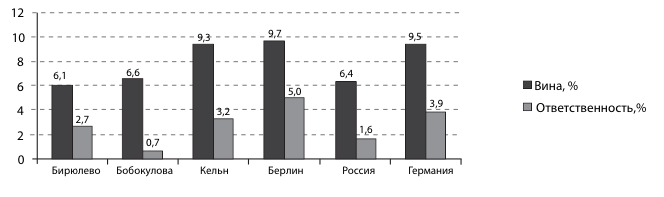
\includegraphics[scale=0.5]{blameAndResponsibilityTweets}
	}
	\caption{Объем твитов с фреймами возложения вины и ответственности, в \% от числа твитов по кейсу/стране}\label{fig:blameAndResponsibilityTweets}
\end{figure}

Гипотеза 2 касалась связи статуса пользователя и адресата обвинения. Как видно (Таблица~\cref{tab:blameAndResponsibilityLink}), в двух из четырех кейсов статус пользователя слабо коррелирует с его/ее мнением о том, кто несет вину за конфликт. Иначе говоря, в половине случаев НКО, государственные акторы и обычные пользователи действительно направляют гнев и обвинения на разных субъектов. Малый объем найденных твитов не позволяет подтвердить Гипотезу 2, но искомая связь очевидна в половине кейсов минимум, при том что в анализ вошли только случаи прямого обвинения и возложения ответственности. Обвинительный дискурс «разлит» в Твиттере в обеих странах, но все же по-разному. Так, в кейсе Бобокуловой, твиты пропитаны дискурсом о вине почти без ее возложения на конкретных акторов. В марте большинство пользователей, включая медиа, называли Бобокулову «няня-убийца» еще до решения суда; в октябре ситуация повторилась, хотя суд отказался назначить Бобокуловой уголовное наказание. При этом в берлинском кейсе водители автобуса назывались подозреваемыми, а не убийцами, даже когда вина тунисца Амира Амри казалась очевидной, что позволило немецким СМИ сохранить лицо при смене подозреваемого.


\begin{table}[ht]%
	\caption{Связь статуса пользователя и адресата возложения вины и ответственности, корреляция Спирмена}%
	\label{tab:blameAndResponsibilityLink}% label всегда желательно идти после caption
	\renewcommand{\arraystretch}{1.6}%% Увеличение расстояния между рядами, для улучшения восприятия.
	\def\tabularxcolumn#1{m{#1}}
	\begin{tabularx}{\textwidth}{@{}>{\centering}m{5cm} >{\centering}m{5cm} >{\centering\arraybackslash}m{6.5cm}@{}}% Вертикальные полосы не используются принципиально, как и лишние горизонтальные (допускается по ГОСТ 2.105 пункт 4.4.5) % @{} позволяет прижиматься к краям
		\toprule     %%% верхняя линейка
		Кейс / страна & Паттерн вины & Паттерн ответственности\\
		\midrule %%% тонкий разделитель. Отделяет названия столбцов. Обязателен по ГОСТ 2.105 пункт 4.4.5
		Бирюлево & 0,010 & "---\\
		Бобокулова & 0,237** & "---\\
		Кельн & 0,136* & 0,182\\
		Берлин & 0,067 & 0,111\\
		Россия в целом & 0,141 (sig. 0,069) & 0,048\\
		Германия в целом & 0,095 (sig. 0,065) & 0,171*\\
		\bottomrule %%% нижняя линейка
		\multicolumn{3}{@{}p{\textwidth}}{%
			\hspace*{2.5em}% абзацный отступ - требование ГОСТ 2.105
			Примечание. Прочерк означает недостаточное количество данных для анализа.
		}\\
	\end{tabularx}%
\end{table}

Гипотезы 3, 4 и 5 касались адресатов обвинения и возложения ответствен- ности в разных странах. Результаты анализа адресатов обвинения и возложения вины представлены для России (Рисунок~\cref{fig:blameAndResponsibilityRussia}) и для Германии (Рисунок~\cref{fig:blameAndResponsibilityGermany}). При этом Гипотеза 3 о том, что в России основным объектом обвинения выступают мигранты, а в Германии "--- госорганы, должна быть отвергнута.

\begin{figure}[ht]
	\centerfloat{
		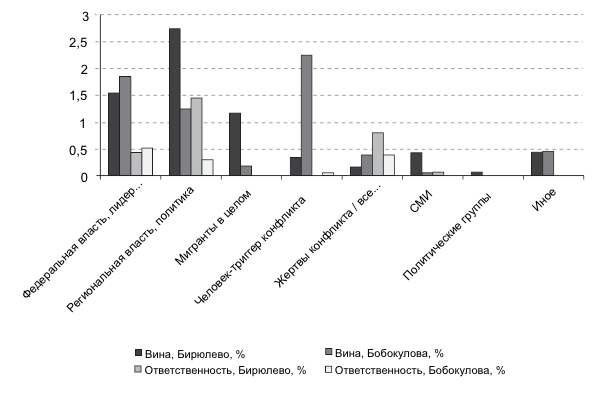
\includegraphics[scale=0.8]{blameAndResponsibilityRussia}
	}
	\caption{Распределение паттернов вины и ответственности, российские кейсы}\label{fig:blameAndResponsibilityRussia}
\end{figure}

\begin{figure}[ht]
	\centerfloat{
		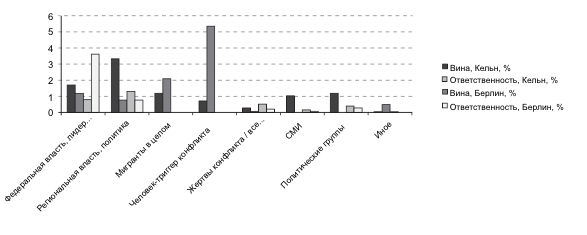
\includegraphics[scale=0.8]{blameAndResponsibilityGermany}
	}
	\caption{Распределение паттернов вины и ответственности, немецкие кейсы}\label{fig:blameAndResponsibilityGermany}
\end{figure}

В конфликтах с групповым триггером наблюдаются сходные паттерны присвоения вины: в обеих странах лидируют региональные власти и по- лиция, затем идет федеральная власть, затем мигранты в целом. Обвинения ложатся либо на лидера страны (особенно на Ангелу Меркель, персонифицирующую политику толерантности), либо на правительство в целом («Правительство готово трусливо спрятаться за овощей-оккупантов, подло предав свой народ "--- лишь бы сохранить власть»). Но наблюдается разница в объеме агрессии по отношению к иммигрантам: в российском Твиттере присутствуют и сарказм, и ноты ненависти, а в немецком "--- сарказм соседствует с признанием своей вины политиками и призывами выяснить, кто все-таки виноват. Также имеется разница в присвоении вины иным акторам. Если в России почти нет обвинений ни СМИ, ни политических групп, то в Германии их объем сравним с объемом обвинений в сторону триггера. В случае Кельна это связано с молчанием СМИ по поводу конфликта и ожиданиями граждан, что СМИ будут более жестко и правдиво освещать роль иммигрантов в нападениях на женщин. Также политическая поляризация и ее отражение в паттернах обвинения очевидно отличает немецкий Твиттер от российского: так, участок дискуссии под феминистским хэштегом \#ausnahmslos («без исключения») снимает вину с мигрантов и перекладывает ее на сексистское общество, в то время как радикальный хэштег \#einearmlaenge, появившийся после рекомендации одного из политиков женщинам держаться «на расстоянии вытянутой руки» от мужчин, использовался для критики не только правительства и политики толерантности, но также феминистских групп. По ходу дискуссии оба хэштега обросли саркастическим дискурсом, противоположным по смыслу. Обвинялись также политические партии "--- как ХДС/ХСС, так и СПД.

В случае Кельна мы могли сравнить медиадискурс с дискурсом «обычных пользователей» (Рисунок~\cref{fig:blameAndResponsibilityKoln}). Видно, что последний является гораздо более жестким с точки зрения наличия обвинений и отличается от первого по структуре. Наибольшую вину пользователи возлагают на политических игроков: федеральное правительство, региональные власти, политические партии, тогда как медиа больше обвиняют полицию (хотя есть и твиты о ее эффективной работе), а также пишут о том, что среди обвиняемых есть иммигранты. Именно пользователи налагают вину на медиа и политические группы, а СМИ обвиняют скорее местные власти и не налагают ни вину, ни ответственность на федеральное правительство.

\begin{figure}[ht]
	\centerfloat{
		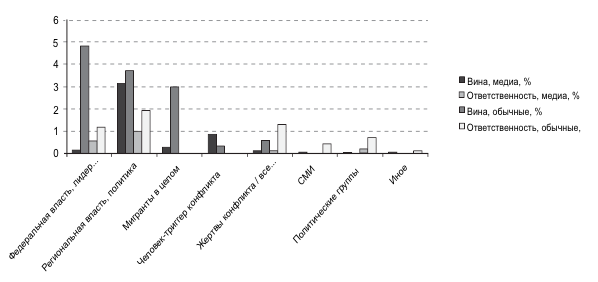
\includegraphics[scale=0.8]{blameAndResponsibilityKoln}
	}
	\caption{Паттерны вины и ответственности в кейсе Кельна: сопоставление дискурса СМИ и «обычных пользователей»}\label{fig:blameAndResponsibilityKoln}
\end{figure}

В кейсе Кельна медийные твиты абсолютно не отражают картину поляризованных настроений пользователей, ограничиваясь констатациями и репортажами о подробностях конфликта. Но и между газетами есть различия: так, только таблоид \textit{Bild} четко указывает, что в насилии в Кельне виноваты иностранцы; СМИ левого спектра, такие как \textit{Sueddeutsche Zeitung} и \textit{Der Freitag}, осторожны в формулировках и нейтральны к иммигрантам.

В конфликтах с индивидуальным триггером паттерн вины иной: основной объем обвинений переложен на виновника/виновницу конфликта, и большую роль в этом в обеих странах играет медийный дискурс, освещающий детали расследования и ареста. Но следует обратить внимание на намного больший объем обвинений в сторону властей в России и в сторону иммигрантских групп "--- в Германии.

Следует признать Гипотезы 3 и 4 опровергнутыми. Реальность дискуссии оказалась противоположна ожиданиям в обеих странах: вина ложится на региональные власти и полицию, а разрешения конфликта люди ожидают от федеральных властей, связывая конфликты с ошибками в миграционной политике. Подтверждена Гипотеза 5: твиты, обвиняющие жертв, во всех конфликтах оказались единичными, а вина и ответственность ложатся на общество, а не на пострадавших. При этом ответственность общества формулируется по-разному. В обеих странах присутствуют радикальные призывы к объединению и «наведению порядка»: «Отвратительные лицемеры! Закончите уже эту \#Asylpolitik! [\#политикуубежища!»] или «Ору папе БЕЙ ХАЧЕЙ! папа в ответ орет из другой комнаты СПАСАЙ РОССИЮ». Однако в Германии также присутствует контрдискурс о необходимости толерантности и снижения уровня сексизма в обществе.

\subsubsection{Заключение}

Вопреки ожиданиям, паттерны наложения вины и ответственности в российском и немецком Твиттере в целом сходны, причем объем обвинений в немецком Твиттере больше. В групповых конфликтах виноватыми признаются федеральная и местная власти и в меньшей степени иммигранты, в конфликтах с персональным триггером "--- зачинщики конфликта. В том, на кого возлагаются вина и ответственность отражается состояние каждого из обществ. Так, в Германии, где медиа и партии активно влияют на миграционную политику, мы видим политическую поляризацию обвинений и выпады в сторону СМИ; но дискурс защиты беженцев и медийный нейтралитет отчасти компенсируют разлом между радикальными феминистками и сторонниками неоконсервативного движения. В российском Твиттере обвинители более солидарны и более агрессивны, а призывы к объединению против неугодных иммигрантских групп ничем не компенсируются, в то время как ожидания, что ситуация разрешится политически ниже в сравнении с Германией.

\subsection{Content Sharing in Conflictual \textit{Ad-Hoc} Twitter Discussions: National Patterns or Universal Trends?}\label{subsec:ch2/sec5/sub2}

\subsubsection{1. Introduction}

In the last decade, online content selection and news spreading proved to be ‘a phenomenon of growing social, economic and political importance’ \cite[p.~331]{LeeMa} capable, arguably, of subversion of traditional media gatekeeping \cite{Carr}. In 2010s, research on factors influencing content sharing has dealt with user motivations and content exposure concepts, among which selective exposure theory shows significant explanatory power; but, till today, these studies provide mixed evidence on which particular factors influence more the selection of shared content, and they remain case-oriented and lack comparative perspectives.

In neighboring research zones, content selection has been studied for decades; thus, of media effects studies, gatekeeping theory is the closest to the studies of content sharing, as it has for long been based on similar sets of research questions. Today, this theory expands to a much greater variety of gatekeeper types, and multi-layer (primary vs. secondary, as well as other divisions) gatekeeping is discussed. But these studies suffer from the same shortcomings; also, the studies do not involve the context of media systems as a variable, while it inevitably casts impact upon the spectra of available content.

This paper aims to partially cover these gaps by analyzing secondary gatekeeping patterns within three Twitter discussions on recent ethnic/racial conflicts in the USA, Russia, and Germany. Here, comparability comes from their \textit{ad hoc} nature \cite{BrunsBurgess} as well as from similarity of the cases in terms of political polarization and policy implications.

Using a specially developed web crawler, we collected the bulk of the discussions, ranged the users by the number of tweets, and assessed the links to outer content in 1,000+ tweets by active users for each case by six variables. In Sect. 1, we present the overview of the research approaches, including primary vs. secondary gatekeeping. In Sect. 2, the cases and the hypotheses are presented. In Sect. 3, we describe data collection, sampling, and coding. In Sect. 4, we provide the results and test the hypotheses. In Sect. 5, we discuss our contribution to the existing research and the limitations of the study.

\subsubsection{2. Explaining Patterns of Content Sharing: Research Approaches}

Today, content sharing encompasses sharing the same content within a platform (e.g. retweeting) and selection and re-publication of media content from outside the platform -- or both, with no distinction in many of published works. Since early 2000s, the researchers have tried to conceptualize and empirically assess the motivations and patterns of content sharing on social media platforms. One of the approaches was uses and gratifications theory which focused on user motives for sharing, finding out that these were, primarily, information seeking, socializing, entertainment, and status seeking  \cite{LeeMa}, especially on online networks as content sharing communities \cite{LeeAntoniadisSalamatian}. Later, network-based approaches added to this evidence that weakly tied users were more likely to share content if they are tied uni-directedly, rather than bi-directedly, thus forming an evidence of content sharing hierarchies in social media \cite{ShiRuiWhinston}

Another research stream tries to identify the factors that influence content selection beyond user motivation. Recently, a range of works tried to check whether the selective exposure theory \cite{SearsPreedman} works for social media -- that is, whether information shared by the users is in line with their values, beliefs, and biases. So far, there is mixed evidence whether this theory works well for content sharing, e.g. on Twitter. For example, authors \cite{ThorsonWells} have shown that, during London riots of 2011, users shared tweets that were in line with their beliefs; in experiment-based research, users do tend to demonstrate bias in news selection \cite{MunsonResnick} -- to the extent of formation of echo chambers \cite{Garett} with the same views reproduced. A group of Italian and American researchers have demonstrated that the selective exposure theory, especially when it comes to personal traits and beliefs, can explain the polarizing effects in echo chambering \cite{QuattrociocchiCaldarelliScala}, consumption of (fake) news \cite{BessiCaldarelliDelVicario}, and in formation of scientific networks \cite{QuattrociocchiAmblardGaleota}. Most echo chambers research is, though, focused on studying in-platform content exchange and its effects (for a review, see \cite{Bessi}), including spreading of online behavior \cite{Centola} and raising issues via collective intelligence \cite{Levy,MaloneKlein}. On the other hand, authors \cite{MorganLampeShafiq} have proved that in sharing news from outside Twitter, users tend to include into their shared links media of various political stands; similar findings were reported for Youtube \cite{HalveyKeane}.

But in both cases, the role of content attracted from outside the platform in formation of user echo chambers remains understudied; we still do not know how this or that piece of content is selected and what makes it attractive enough to break the cross-platform boundaries. Also, being well-grounded in theory, this research remains case-oriented and often lacks comparative component; we try to partly cover this gap.

\paragraph{Content Selection and Gatekeeping.} Mechanisms of content selection for (re)publication were traditionally studied in media effects research, and in particular -- in studies of gatekeeping \cite{White1950}. In general, gatekeeping helps reduce the complexity of the world turning the incoming unstructured information flow into limited and structured sets of comprehensible messages \cite{Singer}. Also, as early as in 1975 \cite{Janowitz}, gatekeeping was associated with objectivity model of journalism based on impartiality and balance, as opposed to advocacy model. But from the very early days of gatekeeping research, it was also considered an oppressive mechanism allowing non-professional intentions in news selection \cite{Mills}.

Media have for decades been studied as major societal information gatekeepers. In 1980s to 1990s, the gatekeeping theory focused on structural constraints of information selection \cite{DonahueOlienTichenor}, of which time and space pressures, professional values, and organizational routines seemed to be more important than the type of platform, thus forming cross-media understanding of news selection priorities. Also, for international gatekeeping, news values theory was used to explain the choice of local/national vs. international news \cite{RobertsBantimaroudis}.

The growth of Internet has drastically changed the gatekeeping landscape. Media institutions felt they were losing monopoly in gatekeeping -- that is, the control over the relationship with the users they had previously prospered with. Industry predictions ranged from alarmist claims of the ‘collapse of gatekeeping’ \cite{WilliamsDeliCarpini} to transformationalism. Among the latter, several ideas deserve mentioning. Thus, the ‘gatewatching’ concept was suggested \cite{Bruns} assigning the users a capacity to transmit information from media without actual participation in content production. Other concepts were ‘network gatekeeping’ \cite{BarzilaiNahon} and ‘audience gatekeeping’ \cite{ShoemakerVos} that described the growing role of information consumers in dissemination of news; soon, these ideas expanded beyond the industry-based structural understanding of ‘gatekeeping layers’, and \textit{secondary gatekeeping} started to be discussed in media studies \cite[p.~6]{ShoemakerVos} \cite{RobertsBantimaroudis,White1950}. Also, today, the gatekeeping theory meets social network analysis where key nodes (users) who either disseminate information themselves or link discussion zones are considered new gatekeepers \cite{JurgensJungherrSchoen} or, rather, gatekeepers with smaller gateways \cite{BastosRaimundoTravitzki}.

Today, three gatekeeping models are most elaborated (for an overview, see [19]). For the first one, authors define five levels of analysis: individual, that of communication routines, organizational, social-institutional, and social-systemic \cite{ShoemakerVos}. For the second \cite{Nielsen}, primary gatekeepers are those ‘who by filtering information and publishing decide what is specifically what we commonly understand as news’; secondary gatekeepers ‘are those that filter already available news content’. Thus, it directly links primary gatekeeping to editorial work, and secondary gatekeeping to content sharing (link-, affinity-, or community-based). The third one \cite{ThorsonWells,WellsThroson} shifts from selection to ‘curation’ of content and suggest five types of curators: journalists, strategic communicators, ‘social others’, computer algorithms, and a reader’s self \cite[p.~35]{WellsThroson}
.
We, though, need to state that we see the distribution of primary/secondary gatekeeping role to be much more complicated than it comes from the current academic debate, and a ‘two-step gatekeeping process’ \cite{Singer} reflecting the idea of two-step communication flow \cite{Katz}, is just one of options. To reduce the complexity, we define them as content producer (‘primary gatekeeper’), content re-publisher (‘secondary gatekeeper’), and intermediary (‘tertiary gatekeeper’). Primary gatekeepers are those who produce pieces of content originally; the content may as well be user-generated. In contrast to this, secondary gatekeepers, when re-publishing, are considering what might be interesting for their core information cocoon. This division seems to be a key one, as their final goals may be similar, as well as factors that shape the individual level of decision-making (from ideology to personality \cite{ShoemakerReese}), ‘resulting in choices that are organizationally efficient and culturally acceptable inside and outside the newsroom’ \cite[p.~56]{Singer}. Tertiary, or ‘algorithmic’ \cite{Napoli} gatekeepers, in their turn, use storage, aggregation, and affinity-based algorithms to shape the overall picture.

What differentiates ‘new’ and ‘old’ gatekeepers is selection principles as part of the ‘content curation’ process. For all of them, the issue of subjectivity in selection has never been resolved: in the 50s and 60s, while it was argued that editors were stuck into the machinery of editorial choice based on vigorous criteria \cite{Gieber}, other authors \cite{Snider,White1950} argued that subjectivity was the basic principle for content selection. With mediatization of society \cite{EsserStromback,Hjarvard}, this gap in understanding has only deepened, as media logic itself has become more subjected to various social pressures, some seen as external for editorial offices and some explicating in subjective editorial decisions. But in online user-level content sharing, user decisions become even more individualized and hectic, also due to combining random/purposeful decisions based on personal traits \cite{Bessi} with the impact of tertiary gatekeepers.

\subsubsection{3. Twitter Discussions as Research Object: The Three Cases}

Of all social media, Twitter has been under researchers’ particular scrutiny due to its bigger feasibility, availability of research software, and platform features. Several works \cite{BakshyRosennMarlow,ShiRuiWhinston} have stated that Twitter is for content dissemination more than other social networks are. Here, we need to discuss how peculiarities of Twitter discussions \cite{ChaBenevenutoHaddadi} and relations between Twitter and the outer media system affect content sharing.

First, we need to acknowledge that replicability of our findings to other discussions may be low due to the \textit{ad hoc} nature of the event-based discussions \cite{BrunsBurgess}. This may lower the comparative potential and be viewed as a natural limitation of this research, even if we have no empirical proof of non-replicability.

Second, the network structure of the discussion, including echo chambers and influencers \cite{BodrunovaBlekanovMaksimov}, may also play a role in content selection -- or, rather, content selection helps shape echo chambers, as it is natural to suggest that the logic of consonant reality \cite{NoelleNeumann} is shows up in all user decisions, including content sharing. In our previous \cite{BodrunovaLitvinenkoGavraYakunin,BodrunovaLitvinenkoBlekanov2016} and ongoing research on Germany and Russia, we have noticed that echo chambers are not only based on attitudes towards immigrants but also on user type. Thus, in Germany in 2014 and 2016, pro-migrant camp is formed around left-liberal media and NGOs, while the pro-nationalist one -- around nationalist leaders in Germany and Switzerland who look like ‘ordinary users’. In the Russian case, under the cover of intense tweeting by media, we discovered a chain of similar pro-nationalist ‘ordinary users’ who also acted as gateways for each other’s content. We may, thus, hypothesize that cross-platform content sharing is linked to the user type, as well as to his/her attitude towards the minority under question.

Third, what may also matter is the difference of media systems and the role of Twitter in them. Russia differs from both Germany and the US in terms of low trust to print media, competitive social media market, and low hybridization of TV. The US and Russian media markets have a distinct online-only segment, while in Germany dominant positions on offline market survive online. All the media systems have relatively high media-political parallelism, and one can trace political alienations in media content and endorsement: progressive/conservative in the US, left/right in Germany, and pro-/anti-systemic in Russia \cite{BodrunovaLitvinenko2013,BodrunovaLitvinenkoGavraYakunin}. As to the Twitter’s position on the media markets, its market niche is a bit bigger in the US than in Germany and Russia; there is lack of substantial research on the comparable user profiling in the three countries.

Thus, we formulate the following RQs: (1) is the pattern of content sharing national-bound or universal? Do established media remain the leading primary gatekeeper for Twitter users in \textit{ad hoc} discussions? Do we see any differentiating impact of the outer media systems upon content sharing? (2) Does the type of secondary gatekeeper correlate with the type of primary gatekeeper? (3) Do personal biases of the secondary gatekeeping correlate with the type of the primary gatekeeper and the views in the attracted content?

\paragraph{The Cases Under Scrutiny.} To better formulate our hypotheses, we will also shortly describe the cases we look at.

In Russia, in October 2013, a Muscovite Egor Scherbakov was, allegedly, killed by an Uzbek immigrant Orkhan Zeynalov; later, Zeynalov was arrested and found guilty. Before the trial, local residents committed repeated bashings of a major warehouse in the Moscow district of Biryulyovo where the migrant community dwelled and worked; they raised against police and formed ‘people’s brigades’ to monitor the local area. The case became the most resonant conflict between Russians and Southern re-settlers in the recent Russian history.

In the USA, in August 2014, a white police officer Darren Wilson shot dead an unarmed African American youngster Michael Brown. Peaceful protest and violent riots rose repeatedly in Ferguson, Missouri, as well as all over the US. The case has polarized American society not only along white/non-white lines but also across political affiliations. 

In Germany, in the New Year night of 2016, mass sexual harassment of women by alleged migrants from Middle East and North Africa took place in Cologne. This made people in many cities protest, mostly under the PEGIDA movement slogans. National media were practically silent on the case, as editorial guidelines prevent journalists from covering ethnics origin of the criminals, while local media reported the case.

\paragraph{Research Hypotheses.} Having stated all the mentioned above, we have formulated the following hypotheses:
\begin{itemize}
	\item H1. Across the cases, an ‘onion’ pattern of content sharing will emerge: social media will be shared most; online-only media will follow, traditional media will come third. In general, structures of media systems will have no visible impact upon content sharing patterns.
	\item H2. The type of secondary gatekeeper will correspond with that of primary gatekeeper in all the three cases.
	\item H3. Personal preferences (pro-/anti-minority) of users will correlate with the type of primary gatekeeper, as well as with pro-/anti-minority bias in shared content.
\end{itemize}

\subsubsection{4. Methodology}

To test the hypotheses, we have collected the discussion content, formed tweets datasets for manual coding, coded them, and made calculations for H1 and descriptive statistics (Cramer’s V) for H2 and H3.

\paragraph{Data Collection.} We have used vocabulary-based web crawling for data collection. To form the vocabularies, we have collected and manually assessed relevant keywords and hashtags at trendinalia.com; all the cases were in Twitter trending topics for at least two days. We have also added keywords found via manual snowballing in 1,000+ popular tweets per case. We used the crawler developed earlier with modules modified for our purposes. The uploading periods included October 1 to 31, 2013 for Russia, August 22 to 31, 2014 for the USA (as the peaking dates of the conflict, August 14 to 21, contained an unfeasible number of tweets for our software), and January 1 to 30, 2016 for Germany. The uploads returned 10715 tweets by 3574 users for Russia, 193812 tweets by 70018 users for the US, and 64874 tweets by 12382 users for Germany.

\paragraph{Sampling of Datasets for Data Annotation.} As we were interested in the active users’ content sharing patterns, we have formed feasible datasets of tweets for assessment based on user lists ranged by quantity of the published tweets. The collections had to be feasible for manual coding, and thus we were seeking the datasets containing around 1000 tweets; for further research, the datasets are to be enlarged. We had to cut the long tail of the discussion, which may have affected the results in terms of the variety of content shared; but the reason for looking at most active users was that they tend to have more stable patterns of posting and content sharing. Thus, our sample is not representative, but randomized sampling would have even distorted the results in a way, as active users are also those who are retweeted more than others \cite{BodrunovaBlekanovMaksimov}, and, thus, the content they share creates impact that goes beyond average.

Cutting the user ‘long tail’ implied establishing a threshold of user activity -- that is, the minimum number of tweets posted in the discussion \cite{Chadwick,MunsonResnick}. Due to very differing user activity, these thresholds (\textit{K} = \textit{Ntweets} per user) differed much: for Russia, \(K = 20\), for the USA, \(K = 66\); for Germany, \(K = 10\); \(K\) was defined as the point where the graph that ranged users stopped to drop significantly from user to user. After that, randomized samples (certain percentage of tweets) from each user were taken depending on the overall user activity in the discussion, to preserve the comparable volume of the datasets: for Russia, 40\%, for the USA, 5\%, for Germany, 30\%. After cutting out irrelevant tweets, replicas, and foreign-language tweets, the final datasets included: for Russia, 1120 tweets; for the USA, 1095 tweets; for Germany, 911 tweets (since many tweets were in English and had to be cut out). The relatively small sample is explained by the fact that reading of media texts could not be automatized, as so far no sentiment analysis or machine-learning techniques could provide for clear understanding of user attitudes.

\paragraph{Coding.} 
Coding. Coding of the datasets was performed by experienced experts and native speakers. Four variables were coded: user type = secondary gatekeeper type (‘ordinary user’/political activist/political actor/hybrid media/online-only media/‘media’ on Twitter/‘culture’/other or non-defined); user’s attitude to minority (neutral/pro/anti/non-defined); type of primary gatekeeper (‘social’, online-only, hybrid media, politics, ‘culture’, other/non-defined); attitude to minority in media content (neutral/pro/anti/non-defined). Links to own content were excluded from the analysis. Also, we excluded the links to Twitter-based photo content (pic.twitter.com). In future, bigger samples may be coded.

\subsubsection{5. Results and Discussion}

On completing the aforementioned procedures, we have received the following results.

\textit{H1.} We have calculated the number of links to content outside Twitter in the three
datasets in absolute figures and in \% (see Table~\cref{tab:datasetLinkNumber}).

\begin{table}[ht]%
	\centering
	\caption{Number of links in the datasets, absolute \(N\).}%
	\label{tab:datasetLinkNumber}% label всегда желательно идти после caption
	\begin{adjustbox}{width=1\textwidth}
		\small
		\begin{tabular}{ c  c  c  c  c  c  c  c  c  c  c }% Вертикальные полосы не используются принципиально, как и лишние горизонтальные (допускается по ГОСТ 2.105 пункт 4.4.5) % @{} позволяет прижиматься к краям
			\toprule
			Country & \multicolumn{2}{l}{\makecell{All links, of all tweets}} & \multicolumn{2}{l}{\makecell{Social media}} & \multicolumn{2}{l}{\makecell{Online-only media}} & \multicolumn{2}{l}{\makecell{Hybrid media}} & \multicolumn{2}{l}{\makecell{Other}} \\
			\hline
			Russia & 159 & \textit{14.2\%} & 62 & \textit{39\%} & 29 & \textit{18.2\%} & 62 & \textit{39\%} & 6 & \textit{3.8\% } \\
			USA & 280 & \textit{25.5\%} & 70 & \textit{25\%} & 96 & \textit{34.3\%} & 67 & \textit{23.9\%} & 46 & \textit{16.4\%}       \\
			Germany & 317 & \textit{34.8\%} & 41 & \textit{12.9\%} & 41 & \textit{12.9\%} & 197 & \textit{62.1\%} & 38 & \textit{12\%} \\
			\bottomrule
		\end{tabular}%
	\end{adjustbox}
\end{table}

In Table~\cref{tab:datasetLinkNumber}, we show political, economic, and cultural links all together, as they are few; everywhere, media are, indeed, the dominant primary gatekeeper, but with very different roles of various types of media. This is why we describe the cases in more detail here.

In the Russian case, we see a picture of rivalry between social and hybrid media -- despite low structural online/offline parallelism and low trust to legacy media in Russia. Thus, the idea of the ‘onion’ pattern of content sharing is not supported; hybrid media are shared more than expected. Social media are represented by blog platforms (Livejournal, Blogspot), the local social network Vkontakte and global Facebook and Instagram, and video hostings (Youtube, Ustream). More interestingly, if we look at online-only and hybrid media in terms of their political bias (and to several political links), we will see that, on Russian Twitter, pro-elite and liberal-oppositional content is shared almost equally, making Twitter much closer an ‘opinion crossroads’ than, e.g., the Russian Facebook, a distinct platform-wide echo chamber, as stated earlier \cite{BodrunovaLitvinenkoGavraYakunin}.

For the American case, we see a picture opposite to the Russian one. Here, only 25\% of the links is to social media and other 24\% -- to hybrid media, while online-only comprise over one third. For America, the ‘onion’ pattern, again, is irrelevant. Also, there are several other features characteristic for the US case. First, all the variety of the mainstream media is shared. The leading print media included \textit{Los Angeles Times}, \textit{The Nation}, \textit{The Atlantic}, \textit{Chicago Tribune}, \textit{USA Today}, \textit{Time}, \textit{The Washington Post}, and \textit{The New Yorker}; of TV, MSNBC, CBS, CNN, and Fox got 2 to 3 links each. Regional media market is well-represented, especially by media of the St.Louis county. Second, there is a striking diversity in formats and political positions of online-only media, many of them being personal or group providers of opinionated writing, grassroots political reporting, and alternative news (like \textit{RawStory.com}, \textit{Madiaite.com}, \textit{Vox}, or \textit{Breitbart}). Some outlets balance between politics and journalism (\textit{TheConservativeFreeHouse}, \textit{ThinkProgress}, \textit{TalkingPointsMemo}, \textit{AmericanThinker}). This diversity is supported by that in political links (8\% of all links) belonging to activist, human-rights, and petition websites. Third, we have found virtually no African American media. Unlike in the tweets, the ‘attracted’ discourse, be it pro- or anti-Black, seems to be shaped by ‘white’ media -- except for Youtube that features eyewitnesses’ views, African American commentators, and rap music in support of Mike Brown.

The German case is the only that proves H1 right, but, again, the ‘onion’ logic does not fully work, as social and online media get equal quantity of links -- both almost five times less than the hybrid media. 26 links, or 8,2\%, belong to political organizations or activists. Surprisingly, 84 of 186 (45\%) of German hybrid media links are to advocacy outlets, but this may be explained by the fact that 70\% of them lead to a right-wing magazine \textit{Zuerst} and are posted by the same user. Of the rest, 46 are supra-regional general-interest and 50 are regional and local general-interest media. The regional distribution is representative enough; the links are not Cologne-centered. Nearly all the big players are also present: newspapers (\textit{FAZ}, \textit{Süddeutsche Zeitung}, and \textit{Die Welt} to \textit{Handelsblatt} and the tabloid \textit{Bild}), news magazines (\textit{Spiegel}, \textit{Focus}), public and commercial TV, and public radio. Due to this, left-right media market polarization reconstructs in the discussion, with right-wing media clearly winning. Online-only media referenced to are also highly politicized. More than half of them (24 out of 41) are the links to advocacy media fostering agendas and news frames alternative to the mainstream media, like \textit{Alternative Dresden News}, \textit{DortmundEcho}, or \textit{Pi-news}.

Thus, our H1 is fully rejected: the ‘onion’ pattern of content sharing is absent. Also, national media systems and the state of civil society seem to have a bigger impact than expected upon the sharing strategies of the users. While in the US and Germany 9\% and 8\% of the links, respectively, belong to political websites, Russian content sharing is depoliticized. What unites all the cases, though, is an ‘opinion crossroads’ in terms of political bias present via media links platform-wide, but it is yet unclear whether it is present within ‘echo chambers’.

\textit{H2 and H3.} To assess correlations between secondary gatekeepers’ types and attitudes to minorities vs. primary gatekeepers’ types and attitudes in their content, we have conducted Cramer’s V for the 4 variables described above. The results are shown in Tables~\cref{tab:gatekeeperTypeVS} and~\cref{tab:gatekeeperAttitideVS}.

\begin{table}[ht]%
	\centering
	\caption{Number of links in the datasets, absolute \(N\).}%
	\label{tab:gatekeeperTypeVS}% label всегда желательно идти после caption
	\begin{adjustbox}{width=1\textwidth}
		\small
		\begin{tabular}{ c  c  c }% Вертикальные полосы не используются принципиально, как и лишние горизонтальные (допускается по ГОСТ 2.105 пункт 4.4.5) % @{} позволяет прижиматься к краям
			\toprule
			& $\ldots$primary gatekeeper type & $\ldots$attitude to minority in primary gatekeeper’s text \\
			\hline
			Russia & 0.220 & \textbf{0.248*} \\
			USA & \textbf{0.183**} & \textbf{0.208**} \\
			Germany &\textbf{ 0.219*** } & \textbf{0.372***} \\
			\bottomrule
			\multicolumn{3}{@{}p{\textwidth}}{%
%				\vspace*{-4ex}% этим подтягиваем повыше
				\hspace*{2.5em}% абзацный отступ - требование ГОСТ 2.105
				Sig.: \(*p \le 0.05\); \(**0.05 < p \le 0.001\); \(***p < 0.001\).
			}\\
		\end{tabular}%
	\end{adjustbox}
\end{table}

\begin{table}[ht]%
	\centering
	\caption{Number of links in the datasets, absolute \(N\).}%
	\label{tab:gatekeeperAttitideVS}% label всегда желательно идти после caption
	\begin{adjustbox}{width=1\textwidth}
		\small
		\begin{tabular}{ c  c  c }% Вертикальные полосы не используются принципиально, как и лишние горизонтальные (допускается по ГОСТ 2.105 пункт 4.4.5) % @{} позволяет прижиматься к краям
			\toprule
			& $\ldots$primary gatekeeper type & $\ldots$attitude to minority in primary gatekeeper’s text \\
			\hline
			Russia & \textbf{0.288***} & \textbf{0.290***} \\
			USA & 0.150 & \textbf{0.350***}  \\
			Germany & \textbf{0.183***} & \textbf{0.401***} \\
			\bottomrule
			\multicolumn{3}{@{}p{\textwidth}}{%
%				\vspace*{-4ex}% этим подтягиваем повыше
				\hspace*{2.5em}% абзацный отступ - требование ГОСТ 2.105
				Sig.: \(*p \le 0.05\); \(**0.05 < p \le 0.001\); \(***p < 0.001\).
			}\\
		\end{tabular}%
	\end{adjustbox}
\end{table}

As we see from Tables~\cref{tab:gatekeeperTypeVS} and~\cref{tab:gatekeeperAttitideVS}, in all the cases, type and attitude of the secondary gatekeeper (that is, Twitter user) weakly but significantly correlates with bias in the shared text -- that is, the hypothesis of selective choice of content is supported in cross-country perspective, and in Germany these ties are the strongest. But at the same time the type of primary gatekeeper (that is, in most cases, media platform) has varying relevance. Thus, in Russia, users of various nature all rely on a variety of media, from hybrid to social, but still choose the content that supports their views; this means they look more at content than stick to their preferred media outlets. In the US, the position of a user towards the minority does not correlate with where a user goes for his/her information supply; it is the particular attitude that will be sought after, and this also may be a sign of occasion-based content consumption and sharing, as there is no stability in linking to the same source. That is, echo chambers in content sharing seem to exist in all the cases, but they are formed via different mechanisms. The type of links seems to be all in all less important for the users than the content, and this supports the idea of active seeking of information rather than ‘information cocooning’ and passivity in content consumption. But, as already stated, this may also support the idea of occasional sharing as soon as the users run into the content that supports their views. This needs further research.

What is also seen is that our idea of collision of the individual and organizational levels of gatekeeping may be supported in future. What we have definitely seen in case of Germany and for several users in the US and Russian datasets is what one may call ‘individual-level filter bubbles’ formed not only via posting but also via content sharing. This may amplify the echo chamber concept, as not only network-level inter-user information exchange but also individual-level filtering leads to the rise of closed-up communicative zones. In our future work, we will try to see in detail which gatekeepers were on which side of the conflict, with bigger samples allowing for better conduct of regression analysis.

\paragraph{Discussion and Limitations.} Several methodological issues rose in the process of dataset formation and coding. Thus, representativeness of the datasets was considered against feasibility, and the decision was to have more users, rather than more tweets from each user, in the datasets, especially because many most active users were posting or retweeting the same tweets multiple times and had to be almost fully eliminated from the datasets. Also, comparability of the cases and the codebooks was discussed; as stated above, the cases were considered comparable due to their political nature, time structure, and main actors involved. But still one needs to realize that the understanding of political cleavages differs much in the three countries, and in some cases bipolarism of the political spectra does not bring a proper solution in judging the content.

We could not always code the ethnic belonging of the users, and this variable was not used in the research. Manual assessment of the datasets shows much bigger presence of African American population on Twitter than migrant population in Germany or Russia (which is nearly 0), but, as we see from the results, this did not affect the results too much -- perhaps due to the structure of the media systems, since they all lack significant representation of the minorities among registered media, and this means that the users share what is available.

And, of course, it was hard not to allow a certain level of subjectivity in coding, but we hope that similarity of the codebooks, cross-checks, and advice from native speakers helped to overcome these limitations.

\subsubsection{6. Conclusion}
In this paper, we have shown that the complexity of gatekeeping in today’s commu- nication flows may be reduced to primary (content producers), secondary (content disseminators), and tertiary (‘algorithmic’) gatekeepers; thus, content sharing patterns shed light onto the relations between primary and secondary gatekeeping.

We have found that national media markets and the state of civil society still help break the cross-national patterns of content sharing on Twitter, and all the variety of views is presented. But at the same time, across cultures, users share the content they solidarize with in their views; but if in Russia and Germany, user bias is linked to the media they consume, in the USA users are more spontaneous in their choice. Thus, the idea of selective content sharing due to bias and user status is supported cross-culturally, but what is shared depends highly on what national arenas offer.

\subsection{Mediatization of twitter? Traditional and online media in ad hoc discussions on inter-ethnic conflicts}\label{subsec:ch2/sec5/sub3}

By 1990s, the scholarly community established consensual understanding that mediatized public sphere \cite{Schulz}. Mediatized public discussions were continuously highly uneven in terms of access to opinion expression \cite{Calhoun}. Among other features, it was privileging institutional players, including political elites and corporations, not only as main newsmakers but also as representatives of conflict sides. Also, media themselves became privileged as well, within the “fourth estate” role conceptualization and due to them being the main nodes in societal communication flows -- and also due to a range of media effects that bring significant distortions and biases to public discussions, gatekeeping \cite{White1950,ShoemakerVos} being one of them. Emergence of Internet seems to have equalized ordinary users to media and other institutional actors in their potential access to online deliberation, but not in their social and political capital \cite{Fuchs}, diminishing offline disparities \cite{Daniels}, political capacities \cite{Chadwick}, or users’ chances of becoming influencers \cite{BodrunovaBlekanovMaksimov,BodrunovaLitvinenkoBlekanov2016} or discussion gateways (Bastos, Raimundo, Travitzki, 2013)\cite{BastosRaimundoTravitzki}.

At the same time, several research streams have been focusing on the concept of mediatization of society, which provides another angle on the roles of established media in wider society. Mediatization research (among many others, see \cite{Hjarvard,EsserStromback2014,HeppKrotz}) shows that the concept of mediatization implies \textit{presence} of media as actors, gatekeepers/gatewatchers, or communication nodes in public discussions as well as \textit{impact} of media content and media logic upon a wide range of social practices, or arenas of mediatization \cite[p.~253]{ThimmDangAnhEinspanner}.

We argue that online user-generated discussion may also be viewed as such a social practice, or arena; not only politics on the whole or religious practices but also the communicative exchange among social media users may find itself under specific impact of established media. Thus, it can be mediatized -- that is, traditional media via their accounts may significantly alter the discussion itself (its topicality, boundaries, length, intensity, or user involvement), reshape agendas, and provide framing. But this, first of all, implies that media need to play significant structural roles within the discussion to be able to alter it. E.g., earlier, media-based public discussions may make us expect that media would be present and active within the discussion and would eventually become influentials/influencers \cite{PattersonGrennyMaxfield,ChaHaddadiBenevenuto} -- that is, highly authoritative users who either create waves of support or link micro-groups in discussion as key gateways \cite{BodrunovaBlekanovMaksimov}.

Another aspect of media presence in the online user discussions is presence via media content dragged into user tweets from outside Twitter. Here, both media hybridization theory \cite{Chadwick} and inter-media agenda-setting theory \cite[p.~113--117]{McCombs2004} allow for posing a question on which media (by type, segment, reach, or location) are popular content providers for Twitter users. In comparative perspective, this would provide some evidence on whether national or universal patterns of media presence dominate. Here, mediatization research neighbors content sharing studies \cite{BakshyRosennMarlow,Singer} and secondary gatekeeping studies \cite{Nielsen}, and we may fruitfully borrow from the latter to enrich the analysis of media presence in Twitter discussions.

So far, structural presence of media on Twitter has been studied in a much more thorough way than the types of content dragged into Twitter discussions. But we see it crucially important to study media’s presence that comes both “from within” and “from outside” Twitter, to be able to measure it in a more efficient way. As several research groups have shown that active tweeting does not always lead to being retweeted and commented, we need to look at other latent ways of casting influence, including sharing content from outside sources.

Such analysis becomes even more important for the discussions of high social relevance like conflicts, natural and anthropogenic disasters, or terrorist attacks, as in such cases people tend to follow news media at least to the same extent as -- or even more than -- authorities’ or rescue agencies’ accounts \cite{ChewEysenbach,Bruns2014}. These situations gather in social media, including Twitter, the so-called \textit{ad hoc} publics where influencer status is hardly predictable, but looking at the two aspects of presence may help define media’s real roles in the discussions.

We use a mixed research design that combines comparative assessment of media activity and media content that the users link to. We look at three similar \textit{ad hoc} discussions in English, German, and Russian (with an in-depth case study of the Russian discussion) to see whether activity of media leads to the influencer status in terms of retweeting and several types of centrality. Our initial assumption is that, first, media will dominate the discussions as active tweeters and, second, that the pattern of dominance will be the same in all the three cases: the biggest mainstream hybrid media will be dominant in both active tweeting and shared content, and the most active media will also become influential by connectivity metrics.

The topicality of the chosen cases is inter-ethnic conflicts, namely Moscow anti-migrant bashings of 2013, Ferguson riots in the US in 2014, and Köln mass harassment in 2016. These cases were selected due to the fact that inter-ethnic conflicts in different countries provide very similar frameworks for online discussions, and, thus, \textit{ad hoc} discussions become comparable, at least in terms of patterns of promoting users to influencer status and content sharing. Also, these conflicts are similar to what Cottle \cite{Cottle2006} has described as “mediatized public crises”; these conflicts all have violent triggers but then they move to public sphere and develop there. So far, the research on media and political conflicts \cite{Cottle,Cottle2006,Horsti,EskjaerHjarvardMortensen} touched ethnicity in several various ways, but mainly it explained how mainstream and diaspora media helped certain social groups in acculturation and integration into host societies, as well as how media frames on war and major conflicts worked in national and translational perspective. But it is still quite rare that smaller-scale and event-based inter-ethnic conflicts become the focus of such analysis, and it is even more rare for comparative studies of online communication.

Another line of research, namely online media and migration studies, provides insights in terms of how media diets of “mediatized migrants” \cite[p.~1]{HeppBozdagSuna} are structured, as well as how media appropriation strategies and media cultures \cite{BaileyGeorgiouHarindranath} may shape the presence of minority voices on social networking platforms. But, again, these studies mostly focus on everyday communicative disparities and mediatization effects \cite{Bozdag}, rather than on whether and how minority\&diaspora actors, including media, succeed (or fail) to shape online public discussions in emergency or conflict situations. Of these discussions, those on Twitter have the shortest reaction-to-event time and the biggest breaking news alert potential, thanks to the brevity of messages and newly-grown habits of institutional tweeting.

Today, Twitter as a communicative platform seems to have a disputable reputation in terms of its political relevance \cite{Fuchs} due to its high volumes of de-problematized discourse and “botization” \cite{SanovichStukalPenfoldBrown}. But still, at least for some researchers, Twitter “can be seen as highly relevant for political exchange and public discourse” \cite[p.~254]{ThimmDangAnhEinspanner}, not only because it works as a news alerts platform, as aforementioned, butalso due to its rapid massive response to crisis events, which suits our research goals. Also, due tofeasibility of Twitter research, there is already a body of case studies of influencers on Twitter (foran overview, see \cite{BodrunovaBlekanovMaksimov}) and of content sharing on Twitter, againstwhich we can assess our cross-national results

To assess the selected cases, we use vocabulary-based web crawling, web graph analytics based on the collected data, and qualitative assessment of selected Twitter accounts and tweet collections. The theoretical premises and limitations, methodology of the study, and our results are presented below.

\subsubsection{Review of Literature}

\paragraph{Twitter publics and media presence in them}
As stated above, it is hard to predict whether traditional disparities in access to opinion expression and deliberative influence are reproduced within \textit{ad hoc} discussions -- and whether media preserve their place as important users within them. In our research, we deal with “issue publics” \cite[p.~422]{Habermas}\cite[p.~108]{BrunsHighfeld2016} -- that is, \textit{ad hoc} discursive constellations \cite{BrunsBurgess} that may grow and dissolve within one heated discussion \cite[p.~74]{Dahlgren} becoming affective \cite{Papacharissi}. Discussions by such publics may not be representative enough for the “calm” periods of Twitter discourse on ethnic tensions.

We analyze the cases that, on one hand, foster ad hoc discussion outbursts by ordinary users based on emotions of both social solidarity and intolerance, thus de-privileging institutional players with their rational discourse. But, at the same time, these cases raise the necessity of verified on-the-ground information, which would empower media (and eyewitness users) within the discussions.

Cha et al. \cite{ChaHaddadiBenevenuto} have drawn attention to the change in understanding of mechanisms of communicative influence, namely to the shift from the classic two-step communication flow theory \cite{KatzLazarsfeld,Rogers} to a more modern approach that emphasizes interpersonal and group factors, including readiness for innovation \cite{DomingosRichardson,WattsDodds}. While both approaches still remain theories lacking solid empirical evidence, the same work by Cha et al. \cite{ChaHaddadiBenevenuto} states that the two-step communication flow idea finds proof on Twitter at large, thus emphasizing the role of conversational mechanisms against content-related mechanisms of communicative influence. This, in effect, may mean that media as established nodes of communication flows should retain their influencer positions despite the quality of audience and discussion itself.

But in some works we find evidence that media disappoint the researchers in terms of their overall presence on Twitter, not speaking of influence. Thus, Bastos and colleagues \cite{BastosRaimundoTravitzki} note that impact of media accounts on Twitter is exaggerated, as “only a small portion of tweets received by ordinary users comes from media outlets” \cite[p.~269]{BastosRaimundoTravitzki}. Cha et al. \cite{ChaHaddadiBenevenuto} note that overall presence of media in Twitter is really low (0.01\%). However, the same authors note that presence of media within the Twitter information flows on major news events is two to six times higher (still remaining low, though). Several studies have shown that, in times of crises, their importance grows further, as Twitter users retweet news sources rather than authority sources or expert opinions. E.g., Chew and Eysenbach \cite{ChewEysenbach} have shown that news websites were the most popular sources of retweets during the H1N1 pandemic. Bruns \cite{Bruns2014}, researching on the Twitter discussion on a major earthquake in New Zealand, shows that, out of top 16 user accounts most commented and retweeted, 11 belonged to institutions, that is, to media, authorities, and “utilities” (mobile operators). Despite the list of top influencers defined this way changes in the immediate aftermath of a tragedy, the list of top influencers remains packed with media and authorities’ accounts. Other works cast some light on why this may happen: thus, Lotan et al. \cite{LotanGraeffAnanny} show that journalists often retweeted their colleagues. At the same time, established media outlets, as An et al. \cite{AnChaGummadi} prove, retain the role of publishing news and stories without much interaction with readers; thus, it is users who actively drag media into the discussion by sharing their content -- either via retweeting tweets posted by media or via linking to media content published outside Twitter. Also, media show the biggest information production capacity, but it is celebrities who are followed most \cite{WuHofmanMason}.

\paragraph{Content sharing and media content shared}
Another stream of literature explores inter-media content distribution and its implications for agenda setting and qualities of public discussions -- from the viewpoint of inter-media impact upon agendas \cite{McCombs2004,HarringtonHighfieldBruns}, in-platform visibility of content \cite{Singer}, and new layers of societal gatekeeping of publicly relevant issues resulting from content sharing practices, or secondary gatekeeping \cite{Nielsen}. But we need to state that current works on Twitter do not pay enough attention to shared media content. Many works are dedicated to estimation of efficacy of news sharing on Twitter by media themselves but not to user strategies and configuration of media presence via shared content. Another bunch of works classifies the core content of tweets or users, without assessing shared content from the viewpoint of media presence.

The literature on content sharing focuses today more on linking user parameters to sharing outcomes and on explaining the driving factors of knowledge diffusion on social platforms \cite{Osatuyi}, including users’ motives for selection of particular content, including media content \cite{LeeMa}. Inside this field, a stream of research examines inter-relations between television or video viewing and Twitter. One work \cite{WohnNa} focuses on the types of content shared simultaneously with TV viewing. The work closest to ours is by Cha et al. \cite{ChaBenevenutoHaddadi} who try to classify content of tweets, types of shared media content serving as a classification parameter. But we have not found any work that would look at media hybridity (web 2.0 / online-only web 1.0 / hybrid) in shared content.

In absence of works that would provide preliminary knowledge on which types of media are more active and popular on Twitter, we have on it two assumptions countering each other. On one hand, mainstream media of hybrid nature (that is, traditional media also present online; see \cite{Chadwick}) usually possess bigger resources than online-only news outlets and, thus, provide exclusive and verified information faster, which gains them dominant positions against online-only media. Then, we know that patterns of power distribution on the Internet tend to more and more reproduce the offline ones. On the other hand, the online audience profile (based on younger, more cosmopolitan and tech-advanced user groups) may favor online media as more relevant to their interests and viewpoints. In the latter case, the structure of media presence would be the “onion” one: social media / online-only media / hybrid media, in descending order. This idea is partly supported, e.g., in the Russian case by the monthly statistics of media use online, as produced by Medialogia rating agency: hybrid media occupy two to three positions only within the top 10 titles most read online -- practically in all monthly lists during last three years. This situation may be described as low structural (online/offline) parallelism on the media market. But anyway we will hypothesize that hybrid media are more referenced to than the online-only ones, as this may be true for the US and German media systems with more established democratic media and higher structural parallelism.

\paragraph{Research hypotheses}
Thus, our hypotheses on mediatization of Twitter discussions of inter-ethnic conflicts are the following:
\begin{itemize}
	\item H1. Media in all the three ad hoc discussions will occupy significant (and comparable) places in the lists of top posting users within the discussions.
	\item H2. Content of mainstream hybrid media will be shared more than that of online-only and social media.
	\item H3. The patterns of media activity and content sharing will be the same in all the three cases.
	\item H4. In all the cases, media that were active on Twitter were also leaders of content sharing.
\end{itemize}

\subsubsection{Methodology}
To test our hypotheses, we needed to select comparable cases, upload the data, and assess the data in several ways. Our judgment on the cases was based on several aspects characteristic for all of them. These aspects included:
\begin{itemize}
	\item a clear inter-ethnic / inter-racial cleavage where a “majority” and a “minority” could be defined;
	\item presence of situational violence (a killing, harassment, street violence etc.);
	\item popular reaction to violence (mass demonstrations, people’s gatherings etc.);
	\item public involvement of federal/state-level/region-level authorities;
	\item public discussion wide enough to reach mainstream media and become national/world Twitter trending topics.
\end{itemize}

Thus, the three cases from Russia (Moscow anti-migrant bashings in 2013, October 1 to 31), the USA (Ferguson riots in 2014, August 15 to 30), and Germany (massive harassment in Cologne in 2016, January 1 to 30) were selected; in case of Ferguson, the exact dates were selected by pre-testing due to feasibility reasons, as the discussion was much bigger than the two others. To collect the Twitter data on the discussions on these cases, we used vocabulary-based web crawling and developed a focused web crawler with changeable modules. As its technical parameters had been described before \cite{BlekanovSergeevMartynenko}, we will not discuss them here. What we need to additionally state is, first, that our crawler is not language-dependent, and thus we could collect data in many languages; second, we consider our crawler to perform better than commonly used software for collection of data, as our software can “retreat” in time beyond the threshold of 900 available tweets set by Twitter. Also, our data collection algorithm ensures that tweets marked as “popular” by Twitter cast no impact upon the result and overcome other well-known limitations of Twitter data collection such as limited number of tweets and limited number of requests to the server per second.

The resulting collections of tweets were represented within non-directed web graphs where users were nodes and linkages between them (retweets or comments) were the edges. Our web crawler collects all public tweets marked by a keyword/hashtag, unlike Twitter Search API-based crawlers freely available on the market, as it uses an algorithm analogous to human unfolding of tweet rolls.

To address the hypotheses, we used the following methods:

\textit{H1. Media in all the three ad-hoc discussions will occupy significant (and comparable) places in the lists of top posting users within the discussions.}

We comparatively assessed the user lists ranged by quantity of tweets and described media found in top20 tweeters for each case.

\textit{H2. Content of hybrid media will be shared more than that of online-only and social media.}

Based on user lists ranged by quantity, we have formed feasible datasets of tweets for assessment. We were interested in the most active users, as they were those who tweeted most. The collections had to be feasible for manual coding, and thus we were seeking the datasets containing around 1000 tweets; later on, the datasets may be enlarged. The sampling procedure implied establishing a threshold of user activity – that is, the minimum of tweets posted within the discussion \cite{LevyWindahl,ChaHaddadiBenevenuto}, but due to very differing user activity these thresholds (\(K = \textit{Ntweets}\) per user) were different in each case: for Russia, \(K = 20\), for the USA, \(K = 67\); for Germany, \(K = 10\). After that, certain percentage of tweets from each user was taken depending on the overall volume of the collected data, to preserve the representativeness of the datasets: for Russia, 40\%, for the USA, 6\%, for Germany, 30\%. After leaving out irrelevant tweets, replicas, and foreign-language tweets, the final datasets included: for Russia -- 1120 tweets, for the USA -- 1060 tweets, for Germany -- 911 tweets.

The datasets were examined on the matter of what content (that from media and other outside sources) was referenced to in the tweets. Self-referential links (that is, links to the user’s own content on other platforms), either by media or by other users, were excluded from the analysis. The media whose content was detected were grouped into three groups: social media, online-only media and web 1.0 news portals, and hybrid media (offline media with online representation portals).

\textit{H3. The patterns of media activity and content sharing will be the same in all the three cases;}

\textit{H4. In all the cases, media that were active on Twitter were also leaders of content sharing.}

Results for H1 and H2 were qualitatively assessed for comparison.

\subsubsection{Results}

\paragraph{H1. Patterns of media activity}
Media in the lists of top users. The lists of top 20 most active users are presented in Table~\cref{tab:top20InConflictDiscussions} where media/journalist accounts are marked bold, while “Twitter media” (accounts created with recognizable “media” purposes) are italicized.

\begin{table}[ht]%
	\centering
	\caption{The top20 most active users in the discussions on inter-ethnic conflicts in Russia, the USA, and Germany, with \textit{Ntweets} indicated for each user}%
	\label{tab:top20InConflictDiscussions}% label всегда желательно идти после caption
	\begin{adjustbox}{width=1\textwidth}
		\small
		\begin{tabular}{ c  c  c  c  c  c  c }% Вертикальные полосы не используются принципиально, как и лишние горизонтальные (допускается по ГОСТ 2.105 пункт 4.4.5) % @{} позволяет прижиматься к краям
			\toprule
			\# & \multicolumn{2}{c}{RUSSIA} &  \multicolumn{2}{c}{GERMANY} & \multicolumn{2}{c}{USA}\\
			\hline
			1 & mynameisphilipp & 187 & Chat\_Atkins & 218 & \textit{\textbf{disetv}} & 4880 \\
			2 & \textbf{ifenews\_ru} & 165 & JoeyGerlach & 137 & gprince1110 & 2199 \\
			3 & BorisALV & 103 & SvenMFGN & 129 & iamemix & 2104 \\
			4 & White\_technolog & 97& DennisEntenmann & 126 & djayyy7 & 1080 \\
			5 & topoprf & 89 & LoveBeatsHB & 80 & deray & 1031\\
			6 & ruspoker & 80 & Juliet777777 & 51 & \textit{HandsUpTO} & 988\\
			7 & masfka & 76 & renben1 & 43 & Nowhydrogen & 568\\
			8 & volya\_naroda & 71 & Greg389 & 38 & Team\_LIBer8 & 549\\
			9 & \textbf{MetroRussia} & 69 & gavthebrexit & 37 & TRJustPassingBy & 493\\
			10 & \textbf{ruvr\_ru} & 67 & \textbf{MatthiasMeisner} & 34 & jlangdale & 419\\
			11 & ipotechniy & 57 & Laatzenietlopen & 34 & \textit{\textbf{News\_LNK}} & 383\\
			12 & \textbf{Mir24TV} & 55 & Rabenzauber & 32 & \textbf{CaccioppoliMike} & 369\\
			13 & \textbf{news\_kavkazcen} & 55 & pumaspucke & 30 & jeffwired & 321\\
			14 & MedvedRu & 51 & KoelleunTschues & 28 & M0HAMMEDWASIQ & 313\\
			15 & NoviniRosii & 49 & LupusLotarius & 27 & KennethaScott & 298\\
			16 & \textbf{krgzr} & 48 & vkenneth\_com & 26 & \textbf{\textit{rightnowio\_feed}} & 294\\
			17 & Estraniero & 45 & montagsdemoGIDA & 24 & Disciple4Lif & 281\\
			18 & ciperovich & 44 & \textbf{2n1f} & 23 & justinstoned & 260\\
			19 & \textbf{\textit{urannews}} & 44 & Antonvlimburg & 23 & ABLVCKGOD & 254\\
			20 & \textbf{\textit{istina}} & 41 & Aluhut\_fuer\_Ken & 22 & AnonFatCat & 252\\
			\bottomrule
		\end{tabular}%
	\end{adjustbox}
\end{table}

Table~\cref{tab:top20InConflictDiscussions} shows the following. The patterns of presence of media in top user lists are very different from country to country. In Russia, hybrid mainstream media (\@lifenews\_ru -- a major corporation of low-mid-market and tabloid media, \@MetroRussia -- the Russian version of the free-of-charge Metro newspaper, TV channel \@Mir24TV and state-funded radio \@ruvr\_ru) are very active, but online-only media (\@news\_kavkazcen, the Twitter representation of the famous pro-Caucasian Kavkaz Center, and \@krgzr -- a social-media-based project with formally “general-interest” but mostly politicized content) are neighboring them. In Germany and the US, to a big contrast, not media but individual journalists (\@MattiasMeisner and \@2n1f for Germany, \@CaccioppoliMike for the US) are most active, and mainstream media lose in activity to all other types of accounts (eyewitnesses, activists, religious and cultural commentators etc.).

\paragraph{“Twitter media” in the lists of top users.} What we have also discovered is that in Russia and the USA, unlike in Germany, “Twitter media” were quite active. As stated above, we call “Twitter media” the accounts that were created to perform media-like functions, e.g. dissemination of information, and have no other platform outside Twitter. As we see, the American Twittersphere has its own media that actively tried to shape the discussion on Ferguson; in Russia, similar accounts are found within the top 20 user list.

\paragraph{H2. Shared content}
As stated above, for qualitative assessment of the links discovered, we grouped them into four categories: social media, online-only media, hybrid media, others. Self-referential links were omitted from the analysis; by self-referential links, we mean clearly identifiable links by a user to his/her/its own content on other platforms. In ambiguous cases, the links were not considered self-referential. Links to Twitter were also omitted from our analysis, as well as links to photos posted via Twitter (pic.twitter.com).

Comparing the number of links discovered in the datasets, we can say that Russian Twitter was virtually twice less mediatized than Germany and the USA (159 vs. 280 and 317 links, or 14,2\% vs. 25,5\% and 34,8\%, respectively). In our cases, more established democracies showed bigger willingness of users to rely on external links. But at the same time the number of non-media links tells another story. Thus, non-media links in Russia were only 6 vs. 46 in Germany and 38 in the USA (3,8\% vs. 16,4\% and 12\%, respectively); that is, the Russian users, when they share content, seem to be a bit more media-dependent than Germans and Americans.

Comparing the structure of media content sharing in the three cases, we see that H2 should be completely rejected, since no country has shown the pattern we expected to see (hybrid media shared most, online-only media second, social media third). Thus, Russia, contrary to expectations, showed that social and hybrid media dominated the users’ attention (62, or 39\%, vs. 29, or 18,2\%, vs. 62, or 39\%). This happened despite the fact that Russia was characterized by relatively low online/offline parallelism and, in 2013, there were quite many online-only media which fostered political agendas. In Germany, the proportion was the opposite (70, or 25\%, vs. 96, or 34,3\%, vs. 67, or 23,9\%), despite firm establishment of hybrid media and their dominance within the online media market. In the US, the constellation, again, differs from the expected one, as social media and online-only media equally (almost 5 times each!) lag behind hybrid media (41, or 12,9\%, vs. 41, or 12,9\%, vs. 197, or 62,1\%).

To explain the differences we have found, we will go deeper into the cases with qualitative analysis. We will describe content sharing in the three cases very shortly, as our main focus is comparative analysis.

\textbf{The Russian case.} In terms of the content referenced to, social media dominate. Users reference to posts in the local social network Vkontakte vs. global Facebook and Instagram, blogging platforms (Livejournal, Blogspot), and video hostings (Ustream, Youtube). A more nuanced picture appears if we assess online-only and hybrid media in terms of their political stance and bias, as well as to political links. We clearly see that, on Russian Twitter, both pro-establishment and liberal-oppositional content coexist; media of both political camps are shared almost equally. This brings the Russian Twitter closer to the idea of “opinion crossroads” than, e.g., the Russian Facebook which works like an anti-establishment (or liberal-oppositional) echo chamber \cite{BodrunovaLitvinenko}. Among pro-establishment/state-owned hybrid media referenced to, one can find TASS information agency, Russia today, Vesti (the news bulletin of the state-owned nation-wide TV channel Rossiya 1), tabloid \textit{Moskovski Komsomolets} and others, while the oppositional/independent side is represented by an even bigger number of media, namely Gazeta.ru, BBC Russian and Slon (online-only) as well as hybrid Radio Liberty, business media holding RBC, \textit{Novaya gazeta}, Echo Moskvy radio station, and TV channel Dozhd (“Rain”), among others.

Politically neutral media are also present, being mostly regional information agencies and papers (\textit{The Moscow News}, Rosbalt, Fontanka, Kolomna Times). It is hard to say which exact media are the most popular, as the figures are too low to search for linkage leaders (those aforementioned reach up to 4 tweets each). Political links form a small but important cluster where the same cleavage between establishment and opposition clearly shows: Kremlin.ru and oprf.ru (the account of Public Advisory Chamber) neighbor Amnesty International, Kasparov.ru and Imrussia.org (sponsored by Mikhail Khodorkovsky). What we also see is that the same Kavkaz Center that was posting actively is linked to (but only once), and that there are no other pro-immigrant voices that users would reference to.

\textbf{The American case.} As shown above, in the Ferguson case, only one fourth of the links belongs to social media and another fourth to mainstream media, while online-only web initiatives encompass over one third of them. For the USA, H2 is also wrong, as, again, the hypothesized scheme of linking to hybrid media seems not to work.

As to the contents, there are several features that stand out in the Ferguson case. First, the most popular media that are linked to are Youtube (31 links), \textit{The Huffington Post} (12), \textit{The Gateway Pundit} (12), and \textit{The Daily Kos} (11); the most popular traditional media, \textit{The Washington Post} and \textit{The New York Times}, make up only to 10 and 6 references, respectively. Facebook and Instagram (9 and 7 links, respectively) add to dominance of online vs. hybrid media.

Second, there is an overall high diversity of media that are represented on the American Twitter by user shares. Thus, all the variety of the national media establishment was the basis for content sharing on the American Twitter. The leading print media were, \textit{i.a., Los Angeles Times, The Atlantic, The Nation, USA Today, Chicago Tribune, The Washington Post, Time, and The New Yorker}. On the other hand, TV channels and networks (CNN, CBS, MSNBC, and Fox) all gained unexpectedly low number of links (2 to 3 each). On the contrary, regional media market was represented quite well: local media from St.Louis county where Ferguson is located received 12 links. Also, 5 links belonged to non-US media (\textit{The Guardian}, BBC, and Russia Today).

Third, there is an even more striking diversity of online-only media, many of them being personal or group initiatives (\textit{JuanCole.com, DaleNapier.com, PatDollard.com, Steyn Online, Taki’s Magazine} or even \textit{3chicpolitico.com}), as well as providers of grassroots opinionated writing and alternative news. Given this, the abovementioned leaders in referencing look not like “someday-grassroots-now-established success media stories” but like “first among many equals”, perhaps just less opinionated than \textit{AmericanThinker, Alternet, ThinkProgress, TheConservativeFreeHouse, PoliticusUsa}, or \textit{TalkingPointsMemo} who try to balance between political advocacy and journalism. Alternative news providers are exemplified, \textit{i.a}., by \textit{Madiaite.com, Vox, RawStory.com}, or, of course, \textit{BreitBart.com}. All in all, online-only media are multiple and diversified indeed in terms of left-right divisions; we witness a highly developed market of online-only opinionated writing initiatives and close-to-journalism practices. This diversity is mirrored by that in political links (23, or 8\%) that belong overwhelmingly to activist, human-rights, and petition websites.

Fourth, despite the diversity of views described above, no African American websites that would provide the viewpoint of this community. There are pro-Middle East and pro-Indian websites linked to, but, unlike in the tweets themselves, representation of African American media is \textit{de-facto} 0 in all the segments. The shared content -- and, thus, the discourse around them -- seems to be shaped by “white” media (of course produced by multi-racial teams). The only exception is Youtube which channels the eyewitnesses’ views as well as opinions by African American commentators. We also cannot help mentioning high visibility of cultural products (like rap compositions to support Mike Brown) within the dataset.

\textbf{The German case.} For Cologne, the logic of H2 works only halfway. As shown above, as online-only outlets and social media gain absolutely equal number of links -- 41, and this figure is almost 5 times smaller than for the hybrid media. 26 links, or 8,2\%, belong to political institutions or activist portals. In 2,5\% of cases, users shared a link to news aggregators, quotes collections, Wikipedia, or Google Maps. Within 197 links to the hybrid media, 11 landing pages belong to non-German media (6 -- Switzerland, 4 -- Austria, 1 -- The New York Times, USA).

Contrary to expectations, 84 of 186 (45\%) of links to the German hybrid media belong to advocacy media outlets; they all position themselves as nationwide sources. But this needs to be judged as a case peculiarity, not the regular picture for Germany, as almost 70\% of these 84 links belong to a right-wing journal titled \textit{Zuerst}. Right-wing views are also presented by the outlets published by Institute of State policy (Institut für Staatspolitik) such as \textit{Sezession} magazine and weekly newspaper \textit{Junge Freiheit} (6 and 7 links out of 84, respectively). All the links to \textit{Zuerst} and \textit{Sezession} are published by one Twitter user who posted 88 tweets with external media links. Every link points to an advocacy media (65 links to two hybrid media, 7 links to two online-only media) or a website of political organization (12 links).

Among the rest, 46 may be recognized as leading to supra-regional media of general interest, and 50 as leading to regional and local general-interest outlets, thus forming a nearly perfect federal/local balance very different from the two other cases. Geography of the links covers a lot of regions, and it is worth noting that the links are not Cologne-centered.

On the supra-regional level, nearly all the big players are found among the shared links. Thus, among newspapers one finds \textit{FAZ, Die Welt, Süddeutsche Zeitung, Die Zeit. taz} and \textit{Handelsblatt}, as well as the tabloid \textit{Bild}. News magazines include \textit{Spiegel}, \textit{Focus}, and \textit{Stern}; public and commercial TV range from ARD and ZDF to N-TV, N24, and 3Sat; public radio links lead to Deutschlandsfunk and Deutschlandsradio Kultur. As it is widely known, the German market of supra-regional mainstream media that we recognize as those that follow the objectivity standards still shows considerable left-right polarization. This polarization reconstructs in the discussion on Cologne, but with right-wing media winning: 9 media are neutral, 4 left-wing and 4 right-wing, but the number of links is 12:13:21, and the media with explicit political preferences get more shares per edition than the neutral ones.

Left-wing advocacy media are, thus, outnumbered: the established left magazine Compact has only 5 links, the newspaper \textit{Neues Deutschland} -- only one. 6 more links point at two sources: Epoch Times, newspaper of Chinese political emigrants (4 out of 84), and a new liberal- conservative magazine Tichy’s Einblick run by a CEO the left-wing Ludwig Erhard Foundation. Online-only media links are also unexpectedly highly politicized: 24 out of 41 of them lead to advocacy media (like \textit{Alternative Dresden News, DortmundEcho}, or \textit{Pi-news}) fostering alternative news agendas.

In Germany, we see an interesting example of how inter-connected chains of opinionated sources are reproduced on Twitter via linkage. Thus, the media network of right-wing political movement “Neue Rechte” (New Right) includes websites \textit{Widerstand} and \textit{DortmundEcho} (7 out of 24 advocacy online media links) and hybrid magazines \textit{Zuerst} and \textit{Sezession}. The share of these New Right media is disproportionally big in our sample but all of them are introduced by only one user, one of the most active ones.

\paragraph{H3. Similarity of patterns of media activity and link sharing}
Both H1 and H2 provide for the conclusion that national context is still the primary definer of the mediatization patterns in social media, including Twitter; the patterns are fundamentally different in several aspects, including percentage of tweets with media links, presence of media in top posting users, and aspects of media market representation. E.g. in Russia media links are present in less than 15\% of tweets, while in Germany they are found in over one third of them.

In terms of media activity, Russia seems more mediatized than Germany and the US, and Germany lacks “Twitter media”, while in case of Ferguson only such “media” were among the most active users. But in link sharing, Russian users are least active, and this shows the picture of media being active but not attractive, and this corresponds to relatively low trust to textual media in the country. Germany is a bit more mediatized than the US, and its pattern definitely favors hybrid media (they comprise over 60\% of all links, and journalists are among the most posting users), while in the US the pattern favors online media. Then, despite all the three countries have relatively high levels of regional autonomy, in Germany we see the balance in representation of nation-wide/local media, while in the US major media dominate and only St.Louis outlets are relevant, and in Russia nation-wide media dominate.

In the US, political opinion is definitely present more in online-only outlets, but in Germany almost half of hybrid media are politicized, and in Russia politicization follows the national pro-/anti-establishment polarization in media that formally declare neutrality, while political opinion media are practically non-existent. As to purely political links, Russia showed remarkable absence of activist and discussion portals, while in the Western democracies they were present in approximately each 35 to 50 tweets. The overall structure of link sharing seems to reflect two main factors: the structure of media trust and the state of civil society in the given country, but this needs more thorough research.

Thus, H3 is also rejected -- but only partly. We can spot several important similarities that may point to the nature of Twitter discussions. First, commercial and cultural portals were insignificant everywhere (despite that in the US musicians were among the most active users), which made mediatization go along with politicization. Second, representation of left-right political divisions was quite significant in all the three countries, which makes Twitter an “opinion crossroads” -- maybe not in terms of the discussion but at least in terms of representation of views. Third, there were practically no links to the media that would represent “the oppressed minority” in each case. Thus, the dominance of “media of the white majority” in shaping the Twitter discourse comes not only through posting (which is contested in the American case) but also through mechanisms of link sharing. Fourth, TV was remarkably absent from both top posting users and from top shared media, while Youtube and other video sharing sites, especially in the US, were among the highly cited media.

\paragraph{H4. Media activity vs. content sharing}
As we clearly see from our results, in no case, active tweeting by media is related to active link sharing. This is even true for Russia where media are among the top tweeters. Thus, doubts must be expressed on whether active tweeting leads to raising the number of links shared by Twitter users. The two aspects of mediatization seem to have no relation to each other. Links are shared according to the traditional structures of media systems and activity of civil society agents.

\subsubsection{Discussion and Conclusions}

In this paper, we have argued that online discussions may also be viewed as mediatized (in terms of the place and impact of established media within the discussion), and thus, studies of content sharing and discursive influencers may be united with mediatization research. If so, mediatization needs to be interpreted two-fold: 1) as presence of media and media-like outlets as actors technically equal to other users, and, thus, their activity, connectivity and SNA-based efficacy parameters may be measured; 2) as presence of media via link sharing -- and, thus, media representation may be measured. In this paper, we have focused on only two metrics, namely posting activity and structure of link sharing. Our main aim was to juxtapose the results to see whether the comparative perspective was at all possible, and to assess the results in comparative perspective.

What we have seen is dominance of national modes of media activity and media link sharing. But there are also interesting similarities in discursive power distribution when we look at right-left and “majority”/“minority” representation. Thus, we have seen that active mediatization was much higher in Russia, while in the USA “Twitter media” were on the rise. In terms of content sharing, no similar pattern was discovered. But in all the cases we have seen “opinion crossroads” to form in political terms, with right media outperforming left in Germany due to activity of just one user. Also, we have seen that active tweeting has nothing to do with what links are shared; this poses a question of the Twitter strategy for media entities.

In conclusion, we could add two things on the limitations of this research. First of all, we recognize well the limitations in sampling and interpretation. Most data collection limitations were overcome by the design of our web crawler, but the qualitative interpretation of the discovered links could have had human-related limitations. But beyond this, we have realized that a conceptual limitation exists, and we will work on this in our further research. When assessing social media links, we were assessing channels, not contents, and sometimes ran into representations of online-only media via, e.g., Facebook. We counted this in as a Facebook link, as for our research the channel mattered more; but for possible content-oriented research it seems necessary to develop an understanding of distinguishing institutional(ized) users from “ordinary people” -- which might be complicated in case of popular bloggers or activists. This is especially true because we have realized that studying structural things does not tell it all, and mediatization of discussions on social platforms may (and should) be studied qualitatively in terms of power disparities and the role of particular channels in opinion formation, but not the way it is often studied (presence of one channel at another one), but within a bigger picture depicting all channels within a discussion. Studying link sharing is one of the ways to reach this goal. We hope that, in future, research on structure of media representation could be linked to studying content, to see what content-related factors shape the sharing patterns on particular channels in cross-country perspective.

\subsection{Political actors in Russian Twitter: Patterns of blaming and responsibility in Twitter discussions on conflicts with post-Soviet immigrants}\label{subsec:ch2/sec5/sub4}

\subsubsection{1 Introduction}

Today, e-governance practices include informal procedures of online communication, and the latter, being facilitated by local and global communicative platforms, becomes a growing and more and more crucial part of e-governing.

One may trace several research areas that deal with the roles of social media platforms within the practices of e-governance. Thus, exploration of the overall democratic efficacy of the online communication tools neighbors the studies where social media become a crucial tool in political crisis management and conflict resolution. As both ‘ordinary users’ and authorities perceive social communicative milieus as the spaces for interpretation of the ongoing crises, in most cases, authorities try to play proactively in social networks and microblogs, including Twitter.

But what is true for advanced democracies may not always be true for transitional ones. Low trust to institutions, lack of practices of public scrutiny, and absence of traditions of accountability affect public demand of responsibility addressed to the authorities. In these terms, we, till today, do not know whether Russia is similar to other countries both in terms of participation of authorities in communication crisis management in social networks and in terms of public claims for action and responsibility addressed to the powerful institutions, as Russian social media remain seriously under-researched. Moreover, studies of Russian-language discourse in social media and microblogs is, beyond several exclusions, virtually absent; these exclusions, though, tell us of gradual radicalization of the Russian social networks, both in terms of language used and presence of radical activists.

We aim at partly filling in this gap by comparative assessment of two conflict-based Twitter discussions related to immigrants from the post-Soviet South (Central Asia and South Caucasus). Our expectation is that, as earlier research shows, the discussions may be politically inclusive in terms of opinions expressed, but they may not include the political actors directly responsible for emergency management. In this paper, we ask the questions about the presence of political actors and radicals in the discussions, as well as the user expectations on conflict resolution.

In Section 2, we provide the literature review on how emergency discussions on Twitter function in other countries. In Section 3, we describe the local research context and the cases we have chosen for analysis. In Section 4, our hypotheses and methodology are explained; in Section 5, the results are stated and discussed.

\subsubsection{2. Literature Review}

\paragraph{2.1 Social media and government: approaches to the role assessment} 
In the recent years, studies of government activities in social media \cite{BarskyTrainorTorres,BertotJaegerHansen,BrunsLiang,CampbellLambrightWells,MendozaPobleteCastillo,Mergel,MergelBretschneider} have followed two major lines of discussion. First, scholars explore efficiency of social media as a tool of democratic participation and engagement \cite{BertotJaegerHansen} and discuss whether social media foster participatory dialogue, engage citizens in public government and co-production of policies, and provide access to the ‘innovation through public knowledge’ \cite[p.~31]{BertotJaegerGrimes}. Social media have become a significant element of e-governance within a very short time period \cite{BarskyTrainorTorres,BertotJaegerHansen,CenterForTechnology,Newman2011,OhKwonRao}, and by their nature, they differ from platforms controlled by governments as to the degree of interactivity and cooperation with citizens \cite{MendozaPobleteCastillo,Mergel}.

The second line of academic literature explores the role of social media in governance practices in cases of emergency \cite{BarashKelly,BrionesKuchLiu,MaciasHilyardFreimuth,PanagiotopoulosBarnettBigdeli}. Emergency management focuses on predicting and preventing incidents of social unrest as well as mitigation of a conflict while the incident or disaster is taking place. Government use social media as a tool for predicting, monitoring, and mediating issues of concern, to ‘provide officials with insights into the perceptions and mood of the community’ \cite[p.~481]{KavanaughFoxSheetz}, to inform and to be informed \cite{GasparPedroPanagiotopoulos,HughesPalenSutton}.

Both authorities and citizens use social media as milieus where interpretation of emergency situations takes place \cite{ComfortWaughCigler,HeverinZach,KavanaughFoxSheetz,Lodge,Osimo,PalenViewegAnderson,ProcterCrumpKarstedt}. Services like Facebook or Twitter were ‘rapidly integrated into disaster environments’ \cite[p.~547]{Comfort}. Social media present a natural platform for information dissemination in the disasters or crises: thus, as early as in case of London subway bombing (2005), social media played an active role \cite{ComfortWaughCigler}. Some researchers have even stated that information flows via social media possess higher potential for engaging between authorities and the public in comparison to other sources of information and deliberation \cite{Crump,SellnowSeeger}.

Correct risk management implemented by the government or local authorities can mitigate public mobilization in an emergency like social unrest or riots \cite{KoltsovaKoltcov,Mileti,SalimovskyErmakova}. Sufficient implementation of communication strategies by the governmental agencies provides community members with ‘timely and reliable information to signal that authorities have the situation under control’ \cite[p.~86]{PalenViewegAnderson}. Community members can develop their own decisions relying on and interpreting this information \cite{ChangKannan,JungPark}. For example, Twitter can be used for collective sensemaking during civil unrest incidents \cite{ReadingTheRiots}, as a warning tool in natural disasters or as means of coping with the stressful effects \cite{DorasamyRamanKaliannan} of food contamination incidents \cite[p.~86]{PalenViewegAnderson}.

\paragraph{2.2 Governance via text in cases of civil unrest: the use of Twitter} 
In general, we may state that relevant studies have shown Twitter’s efficiency in multidimensional communication -- top- down, bottom-up, and lateral -- during crisis events \cite{AlSaggafSimmons,DorasamyRamanKaliannan,HorsleyBarker,HughesPalenSutton}.

Twitter as a channel ‘of timely, actionable and reliable information’ \cite[p.~86]{PalenViewegAnderson} is of vital importance ‘to find, share, and disseminate time-sensitive content such as breaking news and information about unfolding crisis events’ \cite[p.~1]{AlSaggafSimmons}\cite{BrionesKuchLiu,HughesPalenSutton,MengZhangZhao}. In situations that involve high fear and uncertainty \cite{AndrewsFichetDing,HondulaKrishnamurthy,PalenViewegAnderson}, speed and reliability are crucial most importantly for emergency management \cite{BirdLingHaynes,BodrunovaLitvinenkoGavraYakunin,DorasamyRamanKaliannan,ReadingTheRiots,HughesPalenSutton,Noveck,PalenViewegAnderson}. In 2013, Twitter launched a special warning system Twitter Alerts that collects and spreads among users information from authorities registered as sources of official emergency alerts such as police, ambulance, meteorological agencies \cite{PalenViewegAnderson}. Others argue that Twitter provides access to the sources with high level of unreliability \cite{AlSaggafSimmons}. News media and official accounts of institutional users could act as regulators and managers of the information flows \cite{AlSaggafSimmons,JinBrookeLucinda}. Although non-institutionalized actors ‘broadcast more up to date information (and sometimes misinformation) than government organizations and mainstream media’ \cite[p.~483]{KavanaughFoxSheetz}, institutionalized ‘agendas and discussions continue to shape conversation around major news stories’ \cite[p.~6]{MorrisCountsRoseway}.

Twitter provides emergency management agencies with unique possibilities for monitoring and reacting in real time. Traditional methods of monitoring such as surveys do not provide any opportunities for ‘influencing or mitigating events as they evolve’ with that limited period of real time \cite[p.~481]{KavanaughFoxSheetz}. Response time of social media is faster than traditional sources of information \cite{HughesPalenSutton,JungPark,QuHuangZhang}.

Relevant studies focused on the use of Twitter during disasters, mass political demonstrations or riots \cite{HoustonHawthornePerreault,HughesPalen,JinBrookeLucinda} have shown that people use the microblogging platform to disseminate information simultaneously to as many people as possible and they are less likely to search for additional information outside the platform in case of emergency.

Users’ and authorities’ emergency management strategies in social media depend on the type of emergency \cite{PalenViewegAnderson} but the general principles also were revealed by scholars. Users describe the events, condemn the riots, raise donations and express solidarity \cite{GolbeckGrimesRogers}. Authorities try to solve the emergency the fastest possible, to attenuate public stress and avoid the possible escalation \cite{PalenViewegAnderson}.

\paragraph{2.3 Role of emergency management agencies in Twitter discussions}
Within emergency situations, management agencies have a role of an active moderator \cite{BertotJaegerGrimes}. ‘Officials managing social media channels’ \cite[p.~2]{AlSaggafSimmons} release factual information about the situation or activities of the government, disseminate recommendations on safety, encourage the public for more input and ensure the public about law enforcement (with reporting on legal actions). They also spread information provided by other institutional accounts (retweeting police messages), update and comment on sought information or rumors \cite[p.~92]{PalenViewegAnderson}. Moderators validate information and recommend official information and sources \cite{BertotJaegerMunson} via retweets. Official sources play an important role in correcting rumoring \cite{AlSaggafSimmons,OhAgrawalRao}. Thus, during 2011 London riots, local governmental authorities have performed a very active role in the information flow not only posting or retweeting actively but also framing ‘their own Twitter messages to lead public attention to alerts, warnings, updates and proposed actions’ \cite[p.~93]{PalenViewegAnderson}. Official accounts in social media during an emergency are not isolated but act as nodes within an information network \cite{JinBrookeLucinda,PalenViewegAnderson}.

Data from London riots \cite{PalenViewegAnderson} has shown that accounts of the police managed centrally gained more media attention than local police accounts (37\% of retweets made by bloggers, journalists or media organizations vs. 19\% of retweets, accordingly). On the opposite, members of the public were more encouraged to share tweets published by the local police accounts (62\% of retweets by public vs. 40\%). Least active in retweeting police messages was local government (only 2\% of retweets made by local government, from 2\% to 5\% by police) \cite[p.~427]{PanagiotopoulosBarnettBigdeli}.

Three models for police use of Twitter were suggested by Crump \cite{Crowe}: broadcasters recruiting followers with large numbers of followers; local knowledge gatherers, following users who follow large number of other users; community facilitators, encouraging a dialogue between different groups of users \cite{PalenViewegAnderson}.

\subsubsection{3 Inter-Ethnic Conflicts in Today’s Russia and Social Media Research}

The recent history of Russia have seen a rocketing growth of inter-ethnic tensions \cite{BodrunovaBlekanovMaksimov,BodrunovaLitvinenkoGavraYakunin}, with several peaks in 2006, 2010, 2013, and 2016 resulting in violent street anti-immigrant actions in Moscow as well as in smaller localities in the North and South of Russia.

Parallel to this, Runet has remained a virtually non-controlled communication milieu where both radical and liberal views were evolving freely \cite{BarashKelly,SalimovskyErmakova}. So far, the linkages between the growth of social unease towards immigrants from the post-Soviet South (Central Asia and South Caucasus) and the reaction to this process, including conflictual incidents, in social media has been heavily under-researched. To partly cover this gap, we aim at studying Twitter discussions on two inter-ethnic conflicts -- the mass anti-immigrant bashings in the Moscow district of Biryulevo and the case of nanny Gulchehra Bobokulova who killed a 3-year Russian girl in Moscow of 2016.

\paragraph{3.1 Inter-ethnic topics on Runet: freedom vs. extremism}
So far, the research on Russian Twitter remains scarce, and even scarcer is it on conflictual discourse on Twitter. This does not change for quite a long time despite the fact that Twitter in Russia is more popular than in many countries of Europe. Several works published in 2010s create the picture of the Russian Twitter as the place of ‘opinion crossroads’ where political camps are equally and actively represented \cite{Greene,NikiporetsTakigawa}. These findings were partly supported by Berkman Center for Internet and Society at Harvard which, for 2010--2011, as well as in later times, identified mostly topic-oriented clusters in the Russian Twitter \cite{AlexanyanBarashEtling,BarashKelly}.

At the same time, a bigger picture of research on social media in Russia shows that social networks and blogs in the Russian language do not show a lot of interest to ‘ethnic-related’ topics \cite{BodrunovaBlekanovMaksimov,Kapucu}. But at the same time, in absence of pro-migrant discourse that could be initiated by NGOs or local authorities, extremist lexicon and discussions led by nationalist and other radical actors gradually grow in importance \cite{SalimovskyErmakova}.

Thus, our expectations towards the Twitter discussions on the conflicts involving post-Soviet re-settlers in Moscow may be somewhat lower than they would be for other countries in terms of participation of political emergency management actors in the discussion; we may expect that, in their absence or scarce presence, radical actors would play the role of discussion leaders. Our earlier research on influencers on the Russian Twitter \cite{BodrunovaLitvinenkoNigmatullina} shows that this expectation has a certain \textit{raison d’etre}.

What we’re interested in is the following. First, we would like to look at whether political actors (parties, politicians, police, local representatives etc.) take active part in shaping the discourse on emergency -- and who they are. Second, we look at radicalization patterns -- both in terms of presence of radical speakers and salience of calls for negative action against immigrants. Third, we look at patterns of assigning blame and responsibility: we expect that, in possible absence of meaningful representation of efforts by political actors, the users will discuss who’s guilty in the conflict and who needs to resolve it.

We also expect that these aspects of the Twitter discussions may vary from one discussion to another; this is why we comparatively assess two cases united by location (Moscow) but varying by nature (mass/individual).

\paragraph{3.2 The cases of Biryulevo and Bobokulova: the conflicts of varying nature}
We focus on two cases of ethnic-oriented (as well as immigrant-oriented) discussions on the Russian Twitter. We argue that patterns of participation of political actors in the discussion, as well as the patterns of blaming and responsibility loading, may depend on the nature of the conflict. This is why we have chosen the discussions around a mass conflict and an individual crime, to be able to juxtapose the findings.

The bashings in the Moscow district of Biryulevo happened in October 2013, after a killing of a young Muscovite Egor Sviridov by an immigrant from Uzbekistan Orkhan Zeinalov. The events that followed were mass bashings at a warehouse where the local Uzbek community resided, several ‘people’s gatherings’, and repeated police street action including arrests of both migrants and bashings activists and establishment of cordons. We look at October 2013 as the time of active discussion.

The case of Gulchehra Bobokulova is even crueler and at least equally resonant, while it remains an individual crime. In March 2016, Bobokulova who illegally worked at a Moscow family as a nanny killed and beheaded a 3-year-old girl Anastasia, the only daughter in the family. During the first stage of the trial, Bobokulova several times changed the reasons why she committed the crime, from ‘call by Allah’ (which caused allegations of her linkage to extremists) to ‘revenge to Vladimir Putin for bombing Syria’; in the end, the court firmly established she was schizophrenic. The trial has raised a discussion on Twitter, which was particularly important, as mainstream media have formed an agreement on not showing visual materials on the trial and, in some cases, not discussing this issue at all.

We expect that these two cases will provide similar polarization of views, while may foster different levels of involvement of local authorities, police, and other possible emergency managers.

\subsubsection{4 Research Hypotheses and Methodology}

\paragraph{4.1 The research hypotheses}
Having in mind all the stated above, we have formulated the following research questions and hypotheses.

\textit{RQ1.} Presence of emergency management agencies varies according to the scale of mass participation in the conflict. Since people were mobilized to go on the streets in the Biryulevo case only, we should see a clear difference between two cases in terms of presence and behavior of governmental agencies. Thus, we ask: Did official Twitter accounts of authorities belong to the most actively posting users during the primary phase of the Birulyevo bashings and Bobokulova trial?

\textit{H1.} Presence of political actors in the Biryulevo case will be higher than in the Bobokulova case -- both in terms of the number

\textit{RQ2.} If the authorities do not play any active role in an online discussion during the active phase of the crisis, their niche is expected to be taken by radical activists. Thus, we ask: Did Twitter accounts of radical activists belong to the most actively posting users during the primary phase of the Biryulevo bashings and Bobokulova trial?

\textit{H2.} In both cases, we expect that radical activists are among the most active users. We also expect that it is them who call for negative action towards immigrants and immigrant communities.

\textit{RQ3.} We expect that the type of user (institutional belonging, communicative role, and locality) correlates with their reaction to emergency management – whether present or absent. Of the latter, we look especially at who puts to whom the blame for the conflict and the responsibility for its resolution. Thus, we ask: Do the patterns of blaming and responsibility depend on the type of user?

\textit{H3.} The variables of user type (institutional belonging, communicative role, and residence) correlate with the patterns of blaming and responsibility in terms of who is guilty and who is responsible for conflict resolution. We also expect that the blaming patterns will follow the nature of the conflict: thus, in the Biryulevo case, blaming will be put to authorities and the diaspora, while in the Bobokulova case she will be the one to be blamed. But as both cases have reached mass audience as cases related to immigration and Islam, the responsibility patterns will be similar, where the host community will try to make the authorities to be tougher on immigration.

\paragraph{4.2 The methodology and conduct of research}
To answer the research questions and to (dis)prove the hypotheses, we deployed the following combination of methods. First, we used vocabulary-based web crawling for collecting tweets. For this, a special web crawler with adaptable modules has been developed and tested. The tests showed that our crawler collects the discussion (tweets and comments) bypassing the limitations related to Twitter API, as it uses the user-like mode of data collection. This allows for collecting full public tweets, rather than for the data available via Twitter API (like 900 last tweets). Repeatability tests were also made and were successful. We have previously described the web crawling method elsewhere \cite{BlekanovSergeevMartynenko,BodrunovaBlekanovMaksimov,BodrunovaLitvinenkoGavraYakunin}; here, we only provide the details relevant for this paper.

To form the vocabulary, we used a two-step procedure: 1) we collected the discussion-related trending words (as defined by trendinalia.com for each of the discussions); 2) we looked at over 1,000 tweets containing these trending words to find more hashtags and keywords, using the snowballing method. Thus, we used six words in the Biryulevo case and ten words in the Bobokulova case.

Second, out of full tweet collections, we sampled tweets of the most active users and created datasets for manual coding by native speaker coders. For this paper, we provide the results based on small samples of tweets, as this work is still in progress. We code the tweets and their authors, three variables per each. Thus, an individual tweet gets coded by six variables.

The datasets were sampled in the following way. As the discussions varied highly in the amount of tweets posted by the users, we had to establish the thresholds to define who are the most active users, and also create feasible and comparable samples for coding. These two tasks were not easy to combine. To sample the tweet collections, we have used the tactics of user- based random sampling -- that is, sampled a certain percentage of tweets from each user’s individual tweet collection. The threshold for sampling was 40\% of user tweets. Then, we also established the level of activity (by \(N\) of tweets posted during the discussion) to define the list of most active users. As the discussions varied in size very much (the Biryulevo case being several times bigger than the Bobokulova case), we established that the active users for the former case start with 25 tweets per account, and for the latter with 5 tweets per account.

After forming the initial datasets, we cleaned them of replicas, non-Russian-language tweets, and irrelevant tweets (including spam); for Biryulevo, we also cut from the sample the users who had less than 5 tweets remaining. For this case, the active users list includes 38 users with 677 tweets to code. For the Bobokulova case, the list includes 138 users with 536 tweets to code.

Third, the two datasets were coded by experienced coders. The variables for the user type are described as follows:

\begin{itemize}
	\item the user’s institutional status (with growing institutionalization): ordinary user / media, journalists, Twitter media / non-systemic political actors, including NGOs and radicals / authorities and their representatives / other or non-defined;
	\item the user’s communicative role (with growing rationality of the speech): non-eyewitness discussion member / eyewitness / media or journalist / expert or institutional representative / other or non-defined;
	\item the user’s spatial and social localization (with diminishing locality): local host community member / immigrant or diaspora representative / country-level institutional actor / foreigner or foreign actor / non-defined.
\end{itemize}

The variables for the speech patterns are described as follows:

\begin{itemize}
	\item the mood of the speaker: incentive constructive / emotional positive / neutral, ambivalent, or non-defined / emotional negative / incentive destructive. Here, ‘constructive’ stands for solidarity across communities, non-blaming, following legal decisions, and compassion, while ‘destructive’ stands for group divisions, action against people, and markers of otherness;
	\item the blaming pattern: who is to be blamed -- the victim / the murderer / the immigrants / the local host community / the authorities / the whole society / actors outside Russia / no one / non-defined;
	\item the responsibility pattern: who should resolve the situation -- the host community / the immigrants / the authorities / someone external / non-defined.
\end{itemize}

Fourth, the coding was subjected to conducting descriptive statistics. We used Spearman’s rho to see the direction of correlations between the variables, and supported the results by Cramer’s V to double-check their strength.

Our findings are presented below.

\subsubsection{5. Results and Discussion}

The results of the coding demonstrate that Russian Twitter discussions on inter-ethnic conflicts differ substantially from those in the UK, New Zealand, and other countries where Twitter discussions were analyzed.

\paragraph{5.1 The research findings}
\paragraph{H1.} Presence of political actors in the Biryulevo case will be higher than in the Bobokulova case -- both in terms of the number of active users and the number of tweets by them.

The H1 is formally supported by our findings, as accounts belonging to political actors are present in the former case and practically absent in the latter one; but in both cases the presence of official political emergency managers is virtually zero.

Thus, among the 38 users we coded, there are three accounts that may be identified as political: two(!) accounts by the Public Chamber of the Russian Federation and one by a State Duma member Sergey Polozov (a personal account). The Public Chamber is an NGO (but with state funding) that works in the area of human rights and links citizens and state authorities. 1/3 of its members are directly assigned by the President of the Russian Federation, 1/3 represent the Russian regions, and 1/3 belong to other NGOs. The main Twitter account of the Chamber is the only political account that demonstrates a participatory strategy for conflict resolution showing how its members work in the Biryulevo district. The other account works almost as an account of an eyewitness collecting the evidences of the authorities doing some job for resolving the conflict. But this is the only account that is there doing so; Sergey Polozov’s account is full of emotional tweets highly criticizing both the police and the alleged murderer. We even went beyond our sample to check the second group of posting leaders; but within 72 accounts that tweeted 20 times or more, there was only one personal account by a policeman from Nizhny Novgorod.

The same, and even worse, goes for the Bobokulova case. Among the 138 users who tweeted 5 times or more, there are two accounts only that belong to authorities: one is the official journal of Vladimirskaya oblast (Vladimir region), and the other is the official account of the Ministry of Internal Affairs (the police ministry) where two tweets tell the same story of a heroic arrest of the lonely Gulchehra Bobokulova by several policemen.

Thus, we state absence of authorities’ efforts to use Twitter to perform the communicative functions characteristic for their counterparts in other countries; no political crisis management seems to be done via Twitter, one of the most rapid means of information delivery in today’s communicative environment.

\paragraph{H2.}  In both cases, we expect that radical activists are among the most active users. We also expect that it is them who call for negative action towards immigrants and immigrant communities.

The first part of H2 is supported substantially by our findings. Thus, in the Biryulevo case, we see five nationalist accounts (of personal, media-like, and NGO-like nature) among the 38 most active ones, with the overall amounts of tweets as big as 188, or almost 28\% of the whole sample; among the 72 most active accounts, there are two more nationalist Twitter media. The same goes for the Bobokulova case, though to a smaller extent: of 138 accounts, five may be labelled as nationalist, and the amount of tweets is smaller. But it is anyway bigger than the amount of tweets by the authorities.

But the second part of H2 is not supported. When we look at correlations between user type and the user’s mood in the tweets, we see that, indeed, there is a weak but significant link between the mood in the tweets and the users’ institutional status, communicative role, and locality (see Tables~\cref{tab:biryulevoCorrelationData1} and~\cref{tab:bobokulovaCorrelationData}).

\begin{table}[ht]%
	\centering
	\caption{Correlation data for the Biryulevo case: user type vs. user…}%
	\label{tab:biryulevoCorrelationData1}% label всегда желательно идти после caption
	\begin{adjustbox}{width=1\textwidth}
		\small
		\begin{tabular}{ l  l  l  l  }% Вертикальные полосы не используются принципиально, как и лишние горизонтальные (допускается по ГОСТ 2.105 пункт 4.4.5) % @{} позволяет прижиматься к краям
			\toprule
			& …institutional status & …communicative role & …locality\\
			\hline
			Spearman’s rho & \textit{insignificant} & 0,189** & 0,282**\\
			Cramer’s V & 0,171*** & 0,178*** & 0,224***\\
			\bottomrule
			\multicolumn{4}{@{}p{\textwidth}}{%
				%				\vspace*{-4ex}% этим подтягиваем повыше
				\hspace*{2.5em}% абзацный отступ - требование ГОСТ 2.105
				Note. \(p \le 0,05\), ** \textit{is} \(0,05 < p \le 0,001\), *** \textit{is} \(p < 0,001\)
			}\\
		\end{tabular}%
	\end{adjustbox}
\end{table}

\begin{table}[ht]%
	\centering
	\caption{Correlation data for the Bobokulova case: user type vs. user…}%
	\label{tab:bobokulovaCorrelationData}% label всегда желательно идти после caption
	\begin{adjustbox}{width=1\textwidth}
		\small
		\begin{tabular}{ l  l  l  l  }% Вертикальные полосы не используются принципиально, как и лишние горизонтальные (допускается по ГОСТ 2.105 пункт 4.4.5) % @{} позволяет прижиматься к краям
			\toprule
			& …institutional status & …communicative role & …locality\\
			\hline
			Spearman’s rho & 0,209** & 0,238** & 0,239**\\
			Cramer’s V & 0,203*** & 0,180*** & 0,216***\\
			\bottomrule
			\multicolumn{4}{@{}p{\textwidth}}{%
				%				\vspace*{-4ex}% этим подтягиваем повыше
				\hspace*{2.5em}% абзацный отступ - требование ГОСТ 2.105
				Note. \(p \le 0,05\), ** \textit{is} \(0,05 < p \le 0,001\), *** \textit{is} \(p < 0,001\)
			}\\
		\end{tabular}%
	\end{adjustbox}
\end{table}

This may mean that users discussing both conflicts tend have institutional, communicative, and locational gaps between those who express solidarity and those who want more divisions in the society.

But if we look who is calling for negative action against the immigrants, we will see that, in both cases, it is not radical users who call for action, but ‘ordinary users’. To tell the truth, such calls are rare: 21 of 677 tweets in the Biryulevo case and only four in the Bobokulova one, and this difference is easily explained by the fact that these ‘ordinary users’ often perform the role of eyewitnesses -- that is, their reaction is provoked by the ongoing events in Biryulevo. Negative emotions are expressed by mixed audience -- ordinary users, media, and nationalist accounts. But what the latter do most is information dissemination -- the basic function which is not performed by the absent authorities’ accounts -- and posing questions and claims.

\paragraph{H3.} The variables of user type (institutional belonging, communicative role, and residence) correlate with the patterns of blaming and responsibility in terms of who is guilty and who is responsible for conflict resolution. We also expect that the blaming patterns will follow the nature of the conflict: thus, in the Biryulevo case, blaming will be put to authorities and the diaspora, while in the Bobokulova case she will be the one to be blamed. But as both cases have reached mass audience as cases related to immigration and Islam, the responsibility patterns will be similar, as the host community will try to make the authorities to be tougher on immigration.

The H3 is partly supported in terms of correlations between user type and the blaming and responsibility patterns; also, the nature of the case casts significant impact upon the blaming patterns. Thus, for Biryulevo, indeed, who is blaming weakly but significantly correlates with who is blamed (see Table~\cref{tab:biryulevoCorrelationData2}).

\begin{table}[ht]%
	\centering
	\caption{Correlation data for the Biryulevo case: user type vs. blaming and responsibility patterns}%
	\label{tab:biryulevoCorrelationData2}% label всегда желательно идти после caption
	\begin{adjustbox}{width=1\textwidth}
		\small
		\begin{tabular}{ l  l  l  l  }% Вертикальные полосы не используются принципиально, как и лишние горизонтальные (допускается по ГОСТ 2.105 пункт 4.4.5) % @{} позволяет прижиматься к краям
			\toprule
			& User mood & Blaming & Responsibility\\
			\hline
			Spearman’s rho & 0,093* & 0,205** & 0,171**\\
			Cramer’s V & 0,132* & 0,187*** & 0,202***\\
			\bottomrule
			\multicolumn{4}{@{}p{\textwidth}}{%
				%				\vspace*{-4ex}% этим подтягиваем повыше
				\hspace*{2.5em}% абзацный отступ - требование ГОСТ 2.105
				Note. \(p \le 0,05\), ** \textit{is} \(0,05 < p \le 0,001\), *** \textit{is} \(p < 0,001\)
			}\\
		\end{tabular}%
	\end{adjustbox}
\end{table}

There are various actors who are blamed in the Biryulevo case – starting from Orkhan Zeinalov to (and mostly) to immigrants on the whole, the host community, and the authorities, to whom the main amount of blaming is addressed. But in the Bobokulova case almost all the blaming goes directly to the nanny murderer, and Spearman’s rho is insignificant for all the user type variables. At the same time, and also naturally, the amount of blaming is much bigger is the second case (220 tweets vs. 72 tweets for Biryulevo, or 41\% vs. 10,6\%); but for Biryulevo, blaming goes very much along with call for action, while blaming Bobokulova is often limited to calling her a ‘nanny killer’.

As to the patterns of imposition of responsibility, the H3 is, again, disproved. In both cases, there are no significant correlations showing that certain social groups have expectations towards other social groups or institutions. For Biryulevo, the opinion on who should be resolving the conflict is divided almost 50/50 between ‘us the locals’ and the authorities (and in case of ‘us’ is evidently linked with call for negative action), without addressing the immigrant community or the society at large. For Bobokulova, there are almost no expectations or questions on responsibility, except for the pro-state online media hub Ridus which several times tweeted on an initiatve by a State Duma member to execute Bobokulova, as well as a couple tweets from radicals. For this case, the users did not even think of any self-responsibility to prevent such events in future; neither have they addressed the local authorities, diaspora, or immigrants’ host countries. The causes of these unexpectedly ‘absent expectations’ needs further research; but it may be a sign of low trust to authorities in prevention of conditions that lead to the events discussed.

\paragraph{5.2 Discussion}
What we have found may be, all in all, described as the picture of \textit{strategic vacuum} on the part of authorities who bear direct responsibilities for resolving and/or preventing inter-ethnic conflicts in Moscow (and beyond). Just as we expected, in these conditions, radical activists fill in the niche and start leading the discussion -- by not only posting claims or questions but via information dissemination, the key function of the authorities’ communication channels.

At the same time, the politicians who are absent as active strategic players become the figures that are discussed. Thus, for Biryulevo, political establishment representatives, including the highest authorities, were constantly mentioned by the users in negative context. But this is true for mass conflicts, while in the case of a single crime, even if cruel, no responsibility action is expected from the authorities, while there are other types of reactions described in tweets -- e.g., a rapid fall of demand for nannies in Moscow within several days after the beginning of the trial. This means that Muscovites resolve their issues themselves without expecting anything significant from the Moscow authorities.

We realize that these conclusions are based on quite small samples of tweets; we continue working upon larger datasets. We also realize the limitations of human coding that are not deprived of subjectivity and mistakes (this is why all the coding by a particular coder was double-checked by another coder). But we are so far sure that our findings will be supported in future; and that we have discovered a gap in e-governance policies that may deserve consideration by the respective institutions.

\subsection{Politicians Driving Online Discussions: Are Institutionalized Influencers Top Twitter Users?}\label{subsec:ch2/sec5/sub5}

\subsubsection{1 Introduction}

Twitter has been often described in the literature as a user-driven platform where horizontality of user connections puts into question traditional hierarchies of actors who influence the debate; e.g., Twitter dramatically individualized participation in collective actions and social movements \cite{BennettSegerberg,BastosMercea}. According to the studies of digital protest and ‘hashtag activism’, Twitter has enabled longitudinal campaigning that changes structure and content of public discussions \cite{BonillaRosa}. Case studies of Twitter discussions on selected conflicts paid more attention to the content of debate and the character of public communication rather than users participating in the discussion \cite{BonillaRosa,GroshekTandoc}. Also, several important works focused on Twitter activities and strategies of single categories of users -- predominantly communicative elites, like politicians and journalists \cite{BaumannFabianLessmann,LasorsaLewisHolton}. But there is still lack of research on what place such users occupy in \textit{ad hoc} discussions on urgent public matters, whether they regain user attention and authority in the new communicative environment, whether they occupy positions that help organize meaningful discussions, and what lies behind their popularity.

Moreover, there is no consensus among researchers on what kind of users becomes influential and whom to consider an influencer at all, as well as which user metrics one needs to look at to collect a sample of influencers. Our earlier research deals with this issue and offers a framework for selecting top users \cite{BodrunovaLitvinenkoNigmatullina,BodrunovaLitvinenkoBlekanov2016}. In this paper, we apply this approach to assess the political institutionalization of online discussions in cross-national perspective -- that task is, again, under-addressed in current research on social media platforms.

Today’s proliferation of social media comes across cultures and political regimes, and it poses another research question -- whether national traditions of public discussions (or at least some of their features) show up on similar occasions online, or the platform features and limitations make them irrelevant. In this paper, we address this question by comparatively assessing the discussions in Germany (a European democracy), the USA (a non-European democracy), and Russia which shows authoritarian trends in media development, along with other areas \cite{Toepfl2010,Sherstobitov,SmythOates,Denisova,BodrunovaLitvinenko}.

In search of comparable discussions, we looked at three cases of inter-ethnic conflicts that gained national attention and triggered extensive networks of Twitter interactions: the Cologne mass harassment of 2016, Germany, the Ferguson unrest of 2014, USA, and the Biryulyovo bashings of 2013, Russia. All these cases were among national Twitter trending topics and all of them caused nation-wide discussion and social polarization.

For all the cases, we assessed the extent to which the offline user status may change the potential of becoming a Twitter influencer (top user by several parameters); we also looked at the nature of the users that were present in the discussions. In Sect. 2, we present the research framework and literature overview; Sect. 3 provides our research hypotheses; Sect. 4 is dedicated to the methodology and data collection; Sect. 5 pre- sents and discusses our research findings.

\subsubsection{2 Influencers in a Horizontal Network: User Status vs. User Rank in Twitter Discussions}

\paragraph{2.1 Twitter: A Platform for Reciprocal Communication?} The network theory applied in the Twitter studies draws attention to the structure of the Twitter discussion based on weak links and cluster dynamics, the formation of horizontal influencers and various approaches to their analysis, as well as the relationship of the structure and content of tweets in their relation to the type of user.

In comparison to other social networks, Twitter is often characterized by nonlinear dissemination of information \cite{BrunsBurgees2012} and low level of reciprocal relationships \cite{BakshyHofmanMason,Habermas,KwakLeePark} creating of Twitter a picture of quite a loose network of non-reciprocated communication. At the same time, a lot of research has focused on finding communicative disparities and hierarchies of various kinds in this seemingly equal and loose discursive milieu.

Despite the initial horizontal character of Twitter communication, scholars revealed several patterns of hierarchy in relation to user influencer status.

First, users differ in terms of activity: ‘the more active Twitter users frequently engage in gathering and sharing what they perceive to be relevant materials, for example tweeting links to further information (or retweeting relevant posts of other users) to their own followers or to Twitter communities formed around topical hashtags’ \cite{BrunsBurgees2012}. Other authors \cite{BastosRaimundoTravitzki} found that users with higher level of message communication have stronger and more selective influence on the information in Twitter.

Second, although Twitter is seen by scholars as ‘a platform that works on the idea of reciprocation’ \cite{GroshekTandoc}, they have found various types of user inequality in the patterns of reciprocation. Thus, it has been shown that users of one type (for e.g. Twitter accounts of news organizations) usually gain attention from users of the same type (other news organizations) \cite{WuHofmanMason} rather than expand their network to ordinary users. Follower-followee relationships on Twitter may form a kind of relatively stable, long-term network that tends to represent the long-term interests of users \cite{BrunsBurgees2012}.

Third, offline group representation patterns may influence differences in user impact upon how the discussion goes. For instance, as minorities are less connected to social movements, they get lower visibility among the influencers \cite{Juris,Clark,BodrunovaLitvinenko2013}; or, ‘young people from historically underrepresented communities neither experience themselves as members of a singular community on- or off-line, nor uniformly choose to follow or interact online with elites who have emerged as political leaders’ \cite{Clark}. Nevertheless, the optimistic view that is shared by a large group of scholars says that Twitter enables communities by ‘artefacts of engagement -- comments, photos, videos, tweets, and news stories’ \cite[p. 239]{Clark} which, as the same author claims after studying involvement of young people into Ferguson events and online discussions, “provided an avenue into what Dahlgren called the ‘proto-political’” \cite{Dahlgren}\cite[p. 244]{Clark}. Participation in online discussions made this social group also visible to other parts of the community; this was ‘important, as both strong collective identities and strongly felt shared grievances are known to play a significant role in spurring members of one’s extended social networks to consider participating for the first time’ \cite[p. 244]{Clark}. Clark also identifies ‘Black Twitter’ as ‘a space in which counter-publics may form as people find and follow one another, engage in discussions about the meanings of Blackness, and discuss strategies for engaging in political action that arise from those meanings’ \cite[p. 239]{Clark}. But at the same time, this implies that ‘Black Twitter’ in some respect opposes the wider discussion environment and lacks political institutionalization.

Fourth, a lot of research is focused on how the platform features of Twitter and structural peculiarities of the discussions bring certain users to the positions of influencers. The notions of gateway formation \cite{BastosRaimundoTravitzki} and gatewatching \cite{Bruns2011,Bruns2005} demonstrate that networking patterns strongly influence the potential discussion hierarchies. But this research is not that well linked to the offline nature of the users, which till today remains a research gap. Moreover, the nature of Twitter discussions has been also described as ad hoc, which implies that the findings for one discussion are not applicable to another one. But both research on Twitter gateway formation \cite{BastosRaimundoTravitzki} and our own research shows that technical nature of Twitter discussions has stable features that enable comparative research.

And, perhaps most important, several studies of Twitter have linked user rankings and influencer status to their offline metadata. Thus, studies on Twitter segments that belong to the USA and Sweden have shown that experts, professionals, and old-established organizations exert more considerable influence within discussions \cite{FoxZickuhrSmith,Ruth}. In case of emergency, e.g. natural disaster or a terror attack, the so-called utility accounts may start to play a bigger role \cite{Bruns2011}. The same author has also shown that media and politicians belong to influencers on Twitter \cite{Bruns2011}; other works have shown that, for example, Norwegian politicians and journalists share patterns of Twitter activity \cite{EnliSimonsen} but not in all features. E.g. politicians posted significantly more retweets with hashtags than the journalists, and the politicians’ promoted hashtags through retweets, while journalists used hashtags to promote original content \cite{EnliSimonsen}.

Thus, among the various factors that are, arguably, expected to shape growth of a user’s influencer status, beyond the platform and network nature, the most relevant for institutionalized users would be their activity, their belonging to certain types of institutions, their grassroots/systemic status, and their belonging to the majority/ minority. But this has not yet been tested in comparative perspective, including the democratic/non-democratic states.

As it is known from a lot of research on the aftermath of the Arab Spring \cite{Lynch,TufekciWilson}, as well as from other studies on Twitter and authoritarianism \cite{TufekciWilson,HowardAgarwalHussain}, post-communist, semi-authoritarian and authoritarian states may have differing patterns of political use of Twitter, as well as regime responses to it. This creates a perspective for comparing online discussion patterns in democratic, non-democratic, and hybrid or semi-authoritarian countries, to learn how much they actually differ.

\paragraph{2.2 Measuring Influence in Twitter Discussions} 
To dig a bit deeper into the nature of linkages between the offline user status and his/her online influencer status, we need to look at two major research lines that deal with: (1) how influencers are defined; and (2) how online behavior patterns of political actors is linked to their reaching the influencer positions.

As noted above, hierarchization of Twitter users has been documented in many studies, but not that many of them did it in relation to political actors. Moreover, as soon as it concerns political topics on Twitter, the overwhelming majority of the studies include into ‘politically relevant actors’ not only political institutions and parties, individual politicians, and grassroots movements and their leaders, but also media of various kind. We will follow this tradition and further discuss how offline dominance of these communicative actors translates into their online influencer status.

\textit{Defining Influencers.} As we have addressed this issue in our previous research papers \cite{BodrunovaLitvinenkoNigmatullina,BodrunovaLitvinenkoBlekanov2016}, we will now focus on the aspects relevant for the topic of this research only, as well as on the newest literature in the field.

As stated previously, today’s research on Twitter influencers may be divided in two streams. The first group of scholars includes an account or a group of users into influencers on the basis of non-network-dependent metrics such as the number of followers, comments, or retweets. Within this stream of literature, retweets have been marked as the preferred measure for defining who the influencers are -- these users are retweeted both most frequently and most widely \cite{FrebergGrahamMcGaughey,Aquino,SajuriaVanHeerdeHudsonHudson}. ‘An analysis of responses and retweets provides a useful indication of the overall visibility of each account: as discussed, retweets are a means of amplifying the reach of a tweet, and thus of increasing the visibility of a tweet and its sender’ \cite{BrunsBurgees2012,KwakLeePark,BoydGolderLotan,ChaHaddadiBenevenuto}. There even is a classification introduced by authors \cite{LarssonMoe} for the most active users that includes politicians, bloggers and journalists as well as anonymous users and is based on two types of retweeting -- that is, mentions via @ and RT networks.

Diffusion of messages on Twitter has different velocity depending on retweet activity \cite{BastosRaimundoTravitzki} and user status \cite{LarssonMoe,CollianderMarderFalkman}. What is also important is that a retweet is considered to be ‘a form of further disseminating someone else’s message to one’s own network’ \cite{GroshekTandoc,MascaroGoggins}. Measuring number of retweets is about ‘both influence in diffusion and value in market of a tweet’ \cite[p. 792]{LiuShiChen}. A simple retweet is, in most cases, regarded as the sign of solidarization with the position expressed in the original tweet, but we also know that the retweeting practices vary considerably \cite{BoydGolderLotan}. ‘Retweeting users may even see themselves as information brokers, bridging distinct communities of interest by passing on tweets from one network cluster to another’ \cite{BrunsBurgees2012}. In other works, comments and likes, as well as their combinations, are also considered important as influencer markers, but this line of research is definitely smaller.

The second approach measures connectivity (involvement into discussion or in a network) instead of activity. According to this approach, the most influential are those users who have potential in uniting echo chambers in Twitter because they form big nodes in the discussion networks. Most often, to measure this user potential, the metrics of SNA are employed. The clear difference between two approaches is rooted in fact that such SNA metrics as betweenness and pagerank centralities are network-dependent. “Degree centrality is conceptually the simplest one, which is defined as the number of links incident upon a node. Meanwhile, betweenness centrality and closeness centrality are global metrics which more complex but it can better to identify the influential nodes” \cite{Maharani}. A lot of combinations of network measures have been offered by researchers to define the top users; we rely most on (in/out)degree, betweenness, and pagerank metrics for ad hoc discussions \cite{BodrunovaLitvinenkoNigmatullina}.

In our previous research, we have pioneered juxtaposing absolute metrics and network-based metrics, to show that these correlate \cite{BodrunovaLitvinenkoNigmatullina,BodrunovaLitvinenkoBlekanov2016}. In the most recent studies, there have also been attempts to correlate individual indicators, but no more than three \cite{GroshekTandoc}. But this time we aim at linking this research method to the offline user status that we define via user metadata and user descriptions, as well as the content of the accounts.

\textit{User behavior and their influencer status.} Several studies \cite{EnliSimonsen,GrahamBroersmaHazelhoff,LarssonIhlen} have studied peculiar behavior that distinguishes them from average user profiles. Thus, it was shown that politicians and journalists form isolated networks and tend to interact within these circles – which also may be caused by the nature of the Twitter networks themselves, as other studies have found it for other types of users \cite{BodrunovaLitvinenkoNigmatullina,BodrunovaLitvinenkoBlekanov2016}. Thus, more than two thirds of German politicians that actively use Twitter referred to other politicians in their tweets \cite{BaumannFabianLessmann}. On the other hand, for wider audiences, ‘official’ accounts are able to establish themselves as authoritative sources of information, even in the open environments of social media’ \cite{BrunsBurgees2012}. We also know that behavior matters: witty and sharply formulated political tweets, for example, have a great potential of spreading around the network \cite{AelstVanErkelDheer,ParmeleeBichard}. Also, candidates who have a prominent position in the media are generally also the ones who are more popular on Twitter \cite{AelstVanErkelDheer}.

Similar patterns may be found in online behavior of media and journalists. In case of Ferguson, despite having vast following, on average more than a million followers, legacy media journalists and organizations reciprocated by following only small numbers of users and were the least engaging in terms of retweeting and commenting other users \cite{GroshekTandoc}. These signs of traditional communicative hierarchies let journalists and legacy media remain within top popular users as defined via following but in several days were no longer the most influential in terms of generating discussions and gatekeeping information about the Ferguson decision. This is partly explained by their passive activity on Twitter, according to the authors.

Thus, we will try to explore whether patterns of political actors (including media) are similar in cross-cultural perspective.

\paragraph{2.3 Establishing Comparative Perspective: Twitter and Politics in Germany, the USA, and Russia}

To form better our hypotheses, we need to establish a comparative perspective. For this, we will describe the political use of Twitter in the three countries and show that the cases under our scrutiny are comparable.

\textit{Twitter and politics in Germany, the USA, and Russia.} Although Twitter technologically is the same all over the world, societal structure of users, as well as political clusterization and political use of Twitter, differs from country to country.

24\% of US population used Twitter in 2016 (Pew Research Center). It is hard to identify the leaders of the US Twitter for the American audience, as the data that are provided are not country-based; e.g. the third poplar profile belongs to Barack Obama and is followed by 89.5 Mln of users who obviously live all over the world. According to the open data, most popular accounts of US citizens belong to the show business celebrities.

Throughout the recent years, online polarization has been increasing on the US Twitter \cite{GarimellaWeber,CohenRuths}. Support for the Democratic party is more visible on Twitter than that of Republicans (31\% vs. 19\%) \cite{GreenwoodPerrinDuggan}. Almost 60\% of social media users feel irritated while participating in online discussions with users of different political position \cite{DugganSmith}. A very small number of large organizations that have a very large online network of Twitter followers are concentrating the online political voice \cite{HongNadler}. Among members of the US House of Representatives, politicians with extreme ideological positions tend to have more Twitter followers, both left- and right-wing extremists have larger Twitter readership than their moderate peers \cite{HongKim}. Twitter is actively used in the USA in the election periods, as well as in times of nationwide events.

The divergence of users based on race is more significant in the US Twitter than elsewhere. Also, studies showed that education and ethnic heterogeneity are associated with uncivil communication on the US Twitter, while annual household income and unemployment rate were not related to Twitter incivility \cite{VargoHopp}.

Russian Twitter was launched in 2011 and is less popular than the national social networks Vkontakte (desktop monthly reach in June 2016 46 Mln) and Odnoklassniki (desktop monthly reach in June 2016 30 Mln) \cite{TNSWebIndex2016} as well as Facebook (monthly reach in June 2016 14.4 Mln) \cite{Frolova}. Monthly reach of Twitter was about 12 Mln \cite{Frolova,BrandAnalytics}. Kelly et al. have revealed several political clusters within the Russian Twitter in 2010 and 2011. The cleavages between clusters correlated with topics of discussion rather than with social stratification, which is a sign of presence of echo chambers in Russian Twitter \cite{KellyBarashAlexanyan}. At the same time, both pro-government and oppositional political voices are represented in Russian Twitter almost equally, with slight dominance of pro-establishment voices \cite{Greene,NikiporetsTakigawa}. Leaders of the Russian Twitter are TV anchors and politicians: prime minister Dmitry Medvedev and TV showman Ivan Urgant have about 5.5 Mln followers each. Old-established news organizations (\textit{Channel One} and \textit{Vesti}) are followed by 3.7 Mln of Twitter users each \cite{SocialBakers}. Parody microblogs are also highly visible: the spoof account @KermlinRussia gained over 1.5 Mln followers becoming more popular than the official presidential account the spoof was parodying \cite{Denisova2017}. While not a big share of Russian population uses Twitter the platform attracts more politically active users \cite{BodrunovaLitvinenko2013,BodrunovaLitvinenko2015}.

In general, the Russian segment of Twitter is under-researched. The evidence from previous research provides contradictory data on whether Russian Twitter tends to form echo chambers \cite{KellyBarashAlexanyan} or play rather a role of mediator between different views \cite{BodrunovaLitvinenko2013,BodrunovaLitvinenko2015,BarashKelly}. Also, very recently, the number of bots has risen substantially, especially in discussions on political matters, but this was still irrelevant in 2013.

Twitter is also not very popular in Germany. While more than 30\% of German population have created once a Twitter account, in 2015 only about 10\% of German population used this micro-blogging platform actively \cite{MoscaQuaranta}. Leaders of the German Twitter are celebrities -- football and show business stars with about 4 Mln of followers. In comparison to them, most popular media accounts gained about 2 Mln of followers and accounts of politicians attracted less than 400,000 followers.

Among German Twitter users who were politically active in the 2013 elections, almost every third prefers to participate in supportive networks where users always or often agree with others \cite{VaccariValerianiBarbera2016}; thus, German Twitter is tending to form echo chambers and user chains. Political journalists unite in a journalism-centered bubble where political accounts are included since journalists prefer to follow institutionalized users as sources and do not use Twitter for communication with the audience \cite{Nuernbergk}.

This description shows that we may expect higher presence of political actors in Twitter of democratic countries, and these users will be of different nature (institutional as well as grassroots, perhaps more institutional in Germany than in the US). We can also expect presence of all major political powers on Twitter, but their interaction with users will be scarce, as previous research shows.

\textit{The conflicts under scrutiny.} The three conflicts that we have chosen for our analysis include the Biryulyovo bashings of 2013, Russia, the Ferguson unrest of 2014, USA, and the Cologne mass harassment of 2016, Germany. These conflicts were selected due to the fact that they contained clear political elements, were all ethnic/racial-based, provoked massive discussions on Twitter (reaching the national Twitter trending topics), and had similar ad hoc nature in terms of technical organization. Political criteria for selection included the following: the cases had a violent trigger, evoked or revealed major political polarization in the society, caused peaceful protest, and involved institutional political actors and police forces.

In Russia, major anti-migrant bashings happened in September 2013 in the Moscow district of Biryulevo, triggered by an alleged killing of a Muscovite Egor Sviridov by an Uzbek Orkhan Zeinalov and directed to a warehouse where a lot of Central Asian immigrants (mostly illegal) lived and traded. Police and additional military forces had to gather in the area to stop violence; there were claims on the part of attackers that police over-reacted to the events. Later that autumn, peaceful gatherings of local dwellers continued; there were no direct links in change of Moscow policy towards immigration, but the markets and warehouses in the Russian capital have since then been under particular scrutiny of police and immigration officers.

In the USA, an African American teenager Mike Brown was killed unarmed by a white police officer named Darren Wilson. This event provoked major riots not only in the town of Ferguson where the killing happened but also in other cities and towns; peaceful protest spread up to Washington, DC. The case has polarized the audiences; several media reported that more money was raised for Wilson than for the Brown family. For several weeks, protests continued and had minor policy implications on the local level.

In Germany, in the New Year eve of 2016, mass harassment of female celebrators happened on the main square of Cologne; over a 1,000 women self-reported to be affected, and several risked their lives due to firework pieces being directed to them. As police proved, most of the harassers belonged to the re-settled communities from Middle East and North African countries. The conflict provoked nationwide debates but was also characterized by the silence of media for the first few days, as editorial guidelines did not let papers and TV report on the nationality of harassers.

\subsubsection{3 Method}

\paragraph{3.1 The Research Questions and the Hypotheses} Based on what was said above, we formed the following research questions:

\paragraph{RQ1. Is the structure of presence of politically relevant (institutionalized political, grassroots political, and media) users among the influencers similar in all the three cases?}
\paragraph{RQ2. Do politically institutionalized users play bigger role in the discussion than other politically aligned users?}
\paragraph{RQ3. Is offline status of the users linked to their online influencer status, and by which parameters?}

According to the research questions, we have formulated three hypotheses:

\begin{enumerate}
	\item H1. Due to the nature of the civil society in the countries, there is bigger presence of grassroots political users and NGOs in the USA and Germany in the top user lists than in Russia.
	
	\item H2. Due to importance of political actors during conflicts, as well as inertia of traditional hierarchies, users who belong to the current national-scale political institutions form big nodes in the discussion networks -- that is, they are ranked high by degree, betweenness, and pagerank centralities.
	
	\item H3. The position of users in the top lists correlates with the users’ political status. Thus, the more politically institutionalized a user is, the more he is ‘liked’, retweeted, and commented; also, (s)he occupies a higher place in the structural hierarchy of the discussion web graph (higher InDegree, Degree, Betweenness, and Pagerank). As to the OutDegree, it inversely correlates with political institutionalization, as traditional hierarchies are reproduced in the online discussions.
\end{enumerate}

\paragraph{3.2 The Research Methodology} To answer the research questions, we have done the following:
\begin{enumerate}
	\item We conducted vocabulary-based web crawling to collect the discussion content and to analyze their structure. The keywords were selected at www.trendinalia.com, in accordance with hashtags high-rated by this web service that monitor Twitter trending topics around the world in real time environment and diachronically. A special web crawler has been developed to bypass the limitations of Twitter API;
	
	\item We have reconstructed the discussion web graphs to get the data on network-related metrics;
	
	\item We sampled 50 top users based on nine parameters (number of tweets; number of interactions (likes, comments and retweets); centralities -- degree, indegree, out-degree, betweenness, and pagerank); then we merged them in general lists of top users. Thus, if a user was found in at least one single-metric list, he/she was to be found in the merged top user list. As many users were within top lists by many parameters, the final top lists included 205 users for Russia, 205 users for Germany, and 230 users for the USA. The total number of users in the datasets included 3574 users for Russia, 12382 users for Germany, and 70018 users for the USA;
	
	\item We manually coded the users in the lists for their offline status, aiming at showing their growing political institutionalization (from ‘ordinary users’ to ‘institutional political actors’);
	
	\item We used descriptive statistics (Spearman’s rho and Cramer’s V) to see whether the offline user status correlates with the online metrics;
	
	\item We qualitatively assessed the place of political users within the top lists.
\end{enumerate}

\subsubsection{4 Findings}


\textit{H1. Due to the nature of the civil society in the countries, there is bigger presence of grassroots political users and NGOs in the USA and Germany in the top user lists than in Russia} (Table~\cref{tab:topTierListUserStatus}).

\begin{table}[ht]%
	\centering
	\caption{User status in the top user lists}%
	\label{tab:topTierListUserStatus}% label всегда желательно идти после caption
	\begin{adjustbox}{width=1\textwidth}
		\small
		\begin{tabular}{ l  l  l  l }% Вертикальные полосы не используются принципиально, как и лишние горизонтальные (допускается по ГОСТ 2.105 пункт 4.4.5) % @{} позволяет прижиматься к краям
			\toprule
			& \makecell[l]{Germany\\\(N=230\)} & \makecell[l]{Russia\\\(N=205\)} & \makecell[l]{USA\\\(N=205\)}\\
			\hline
			Ordinary people & 48.70\% & 36.59\% & 27.32\% \\
			Activists and politically active bloggers & 10.87\% & 13.66\% & 23.41\% \\
			Media & 23.48\% & 22.93\% & 17.56\% \\
			Political actors outside state institutions & 1.74\% & 3.41\% & 3.41\% \\
			\makecell[l]{State authorities of any level and their individual\\representatives} & 3.48\% & 6.83\% & 0.49\%\\
			Arts people, celebrities, and experts & 6.96\% & 3.41\% & 13.66\% \\
			Other/non-defined/irrelevant & 4.78\% & 13.17\% & 14.15\% \\ 
			\bottomrule
		\end{tabular}%
	\end{adjustbox}
\end{table}

The biggest share of grassroots political users is present in the USA -- almost 25\% of our sample in comparison to 11\% in Germany and 14\% in Russia. In Germany, many ordinary users have a clear political position that can be understood from their tweets but they don’t define themselves as activists. Despite the share of authorities is bigger in Russia than in Germany, the level of authorities should be taken into consideration. While the sample of Russian political users includes low-level politicians -- deputies of local councils or executives, as well as institutionalized party members outside the State Duma, the list of influential German Twitter users includes a member of the European Parliament, former Federal Minister of Justice and Consumer Protection, and members of parliamentary parties. 50\% of politicians belonging to the German Twitter influencers represent the right-wing party Alternative for Germany (AfD). Thus, H1 is partly supported for the US and Russia.

\textit{H2. Due to importance of political actors during conflicts, as well as inertia of traditional hierarchies, users who belong to the current national-scale political institutions form big nodes in the discussion networks -- that is, they are ranked high by degree, betweenness, and pagerank centralities.}

H2 is not supported for the United States, since there are no state authorities of any level and their individual representatives among users ranked high by degree, betweenness, or pagerank centralities. For Germany, it is partly supported, since there are representatives of ‘Alternative for Germany’ (rating 11 out of 50 by betweeness and 44 by pagerank), ‘Die Linke’ (The Left Party -- rating 33 by degree) and the Social Democratic Party of Germany (rating 41 for degree).

Representatives of state actors are much more authoritative on the Russian Twitter. There are 7 of them that were ranked high by degree (50\% of this type of users in the whole sample), 4 ranked high by betweenness and 8 ranked high by pagerank

Among these users, one is the member of Committee on Drug Prevention by the Federation Council, upper house of the Federal Assembly of Russia (6 by degree, 10 by betweenness, 15 by pagerank). Beside him, the three users also were ranked high by all the three metrics: a member of the Council of the youth wing of the ‘United Russia’ party, an account of the Civic Chamber of the Russian Federation and a member of a populist Liberal Democratic Party of Russia.

\textit{H3. The position of users in the top lists correlates with the users’ political status. Thus, the more politically institutionalized a user is, the more he is ‘liked’, retweeted, and commented; also, (s)he occupies a higher place in the structural hierarchy of the discussion web graph (higher InDegree, Degree, Betweenness, and Pagerank). As to the OutDegree, it inversely correlates with political institutionalization, as traditional hierarchies are reproduced in the online discussions.}

What we see from Table~\cref{tab:userStatusRhoCorrelation} is the following. First, for Germany and the USA, we see a similar pattern. The growth of the level of political institutionalization correlates with absolute figures of user activity, namely likes and retweets -- that is, political figures tend to maintain authority and keep the audience’s wish to interact with their content. This is a sign of traditional hierarchies still being in place in online discussions; belonging to an institution linked to politics slightly raises the chances to be more times liked and retweeted -- but not commented, which also shows that the nature of the discussion is not dialogue and the politically institutionalized users do not tend to enter discussions and generate mutual commenting. This is also partially supported by the fact that there is no correlation between user status and betweenness centrality -- that is, politically institutionalized users do not tend to be linking groups of users more than others, which they could do if talked to people more.

\begin{table}[ht]%
	\centering
	\caption{Spearman’s rho correlating the user status to…}%
	\label{tab:userStatusRhoCorrelation}% label всегда желательно идти после caption
	\begin{adjustbox}{width=1\textwidth}
		\small
		\begin{tabular}{ c  c  c  c  c  c  c  c  c }% Вертикальные полосы не используются принципиально, как и лишние горизонтальные (допускается по ГОСТ 2.105 пункт 4.4.5) % @{} позволяет прижиматься к краям
			\toprule
			& …likes & …retweets & …comments & …Indegree & …OutDegree &…Degree & …Betweenness & …Pagerank \\
			\hline
			USA & 0.299** & 0.235** & -- & 0.214** & \(-0.179\)* & -- & -- & -- \\
			Germany & 0.145* & 0.231** & -- & 0.150* & \(-0.227\)* & -- & -- & 0.189** \\
			Russia & -- & -- & -- & 0.257** & -- & 0.231** & 0.153* & 0.288** \\
			\bottomrule
		\end{tabular}%
	\end{adjustbox}
\end{table}

Also, for the USA and Germany, we see clear support of the idea that political institutionalization raises the number of users who interact with the given user (by InDegree metric) and diminishes the number of users who are interacted with on the part of the given user. In other words, if you belong to a political institution, you post information that people tend to like and share, and you remain attractive for more users than average, but you tend to be passive in communicating with them. This is another sign of traditional hierarchies rising in the ad hoc discussions where all the users are seemingly equal. In Germany, political users also show higher authority among the most authoritative users (by pagerank centrality), but we explain this by the nature of the case and the top user list -- while in Ferguson there were almost no politicians at all, in Germany their presence was bigger and they could enter the ‘authority chain’ of users with high pagerank centrality.

In Russia, by sharp contrast, we see that political users, despite their relatively massive presence, do not create the picture of being different from ordinary users in terms of user attention (likes, retweets, or comments), but the structure of the discussion still makes them different from the average user. They are not only referenced to by more people (not because of content, it seems, but because of their status), but the people who reference to political actors also tend to be more authoritative. It even seems that institutionalized users form something like a self-referential cluster of the discussion, with external audience seeing also referencing to it. This looks like another form of keeping hierarchies – based not on political individual but on political status itself.

But anyway, in all the three countries, politically institutionalized users do not stand in the position of linking people in the discussions and forming circles of interest around them – only in Russia their betweenness centrality is slightly connected to the user status but the correlation is really weak. This may be the sign of the situation when, while traditional hierarchies still work in people’s minds, the real role of political actors in public discussions is not that significant.

These findings are partly supported also by Cramer’s V metric (see Table~\cref{tab:userStatusVCorrelation}) -- with the difference for Germany where there are practically no significant correlations that would show up. But for the USA and Russia correlations not only are there but are really strong, showing the differences between content-based and status-based nature of influencing the discussion by politically institutionalized actors in the US and Russia, respectively.

\begin{table}[ht]%
	\centering
	\caption{Spearman’s rho correlating the user status to…}%
	\label{tab:userStatusVCorrelation}% label всегда желательно идти после caption
	\begin{adjustbox}{width=1\textwidth}
		\small
		\begin{tabular}{ c  c  c  c  c  c  c  c  c }% Вертикальные полосы не используются принципиально, как и лишние горизонтальные (допускается по ГОСТ 2.105 пункт 4.4.5) % @{} позволяет прижиматься к краям
			\toprule
			& …likes & …retweets & …comments & …Indegree & …OutDegree &…Degree & …Betweenness & …Pagerank \\
			\hline
			USA & 0.925** & 0.944** & 0.915** & -- & -- & -- & -- & -- \\
			Germany & -- & -- & -- & 0.813** \textit{(sig. 0.055)} & -- & -- & -- & -- \\
			Russia & -- & -- & -- & 0.716*** & -- & 0.747*** & -- & 0.980*** \\
			\bottomrule
		\end{tabular}%
	\end{adjustbox}
\end{table}

Thus, we see our hypothesis is partly supported for Germany and the USA; there is the pattern of attention growth for more politically institutionalized users there, based on the number of users who pay attention to politicians, as well as on their content which users find sharable in the crisis situations. In Russia, on the contrary, the pattern is not there, and the discussion first seems more deprived of hierarchies, but the structural metrics reveal that the status itself matters -- arguably, more than content these user post. This leads us to the conclusion that political presence in Twitter in democratic countries differs from that in post-authoritarian ones, especially in terms of what creates the authority.

\subsubsection{5 Conclusion}

Thus, we see that even preliminary research like ours shows that there are significant gaps in political representation within conflictual discussions on Twitter; there is room for significant improvement in terms of discussion engagement of political actors, including media and grassroots politicians.

We also see that the USA and Germany tend to differ from Russia in terms of how exactly the hierarchies are reproduced -- in Russia, it is the status itself that matters, and the more politically institutionalized a user is, the bigger chance is that he/she will form an important network node, while in the US and Germany we see that content matters more, but political users fail anyway to be discussion centers.

This provides new grounds for further research on behavior and role of politically aligned users on Twitter.

Of course we see many limitations in this kind of research; also, we have not provided in-depth analysis of the strategies of political actors and the causes that lead them to the detected (and relative) failure in uniting the user groups and discussion echo chambers. But this lies a bit beyond the scope of this paper and demands further research. What we would like to underline is that the divergent patterns of political influencing may be grounded not only in the nature of the national publics but also the nature of the national political arenas.

\subsection{A Self-Critical Public: Cumulation of Opinion on Belarusian Oppositional YouTube before the 2020 Protests}\label{subsec:ch2/sec5/sub6}

\begin{displayquote}
	My friend! You’re a major, aren’t you! You get it all! Stop the guys! To our beautiful sky! Forests! Fields! <…> I love my country so much! You too! You understand everything! Stop the guys! We have such a chance! We all have! We are for the truth! Power is in the truth! Stop the guys! And we will owe you! We, like you, are all Belarusians! Let's try to live the truth!
\end{displayquote}

These words by an anonymous protester addressed to a special forces major were pronounced during the Belarusian street protest rally on the night of 10 August 2020, after the presidential elections, won by official vote count for the sixth time by Aliaksandr Lukashenka. The quote was publicized by \textit{Nexta}, a Belarusian oppositional media now existing as a complex of Telegram channels but, in 2018, mostly active on YouTube. Starting from the election eve, the popular protest rose in Belarus; from that moment on, \textit{Nexta}’s number of subscribers on Telegram grew in a rolling manner in real time for several days, soon reaching nearly 2 million users. This, for a 9.5 million Belarusians (even with the Belarusian diasporas and \textit{Nexta}’s international followers), was an absolute record.

Such growth did not start from scratch. In the 2010s, Belarusian opposition was perceived by many as relatively disunited and existing only “off-system,” without casting any impact upon political decision-making. The formally oppositional parties in the parliament were built into the system of power and mostly supported the status quo. The non-systemic opposition found its shelter on social media, including \textit{Odnoklassniki.ru} (“Classmates”), Twitter, and later YouTube and Telegram. In 2018 and 2019, Belarusian YouTube contained several Minsk-based and regional oppositional channels that contributed to preparing the soil for the post-election protest.

The quote above mirrored a strikingly peaceful mood of the Belarusian protesters who continuously emphasized that the protests were against a particular person and the regime associated with this person, not against fellow citizens. During the rallies, the protesters carried both the white-red-white symbols of the independent Belarus of 100years ago and the current Belarusian post-Soviet flags, underlined the right of the regime supporters to hold their own rallies, brought flowers to the police, and took off shoes if they climbed upon benches. This made both international and domestic observers wonder what the Belarusian oppositional public and the consensus behind it were.

The protest seemed to touch various social groups, from plant workers to students, housewives, and owners of small businesses. Despite this, the public behind it was not amorphous, mostly because it was networked. On social media including YouTube and Telegram, the protesters discussed electoral agendas and protest facilitation, as well as criticized organizational patterns of everyday life and “mundane” discontent related to them \cite{SmoliarovaBodrunova}, and such discussions were clearly making the discussants a critical public \cite{Toepfl}. However, their discourse differed substantially from both policy-critical and leadership- critical publics, as conceptualized by Toepfl for (semi-) authoritarian public spheres.

In this article, we aim at partly covering a gap that exists in studying autocratic public spheres and publics, including those of Belarus. To find out the features of the oppositional public that existed in Belarus before the protests, we collect and analyze YouTube comments to the popular Belarusian oppositional accounts and connections between their authors for the whole of 2018. The six YouTube accounts, \textit{Nexta} among them, were selected with the help of YouTube statistics, expert evaluation by Dr Aliaksandr Herasimenka (University of Oxford, United Kingdom, as for 2021), and discussions with local activists. The number of the collected comments was 120,411 and the number of commenters was 34,770.

First, we assess the commenters’ interconnectedness, in order to define their formal structure as a closed-up community, random-user conglomerate, or a group with a more complex structure. Second, we look at the core group of cross-commenters and discursive features of their comments, including orientation to dialogue, aggression, and antagonism/agonism. Third, we ask whether this discussant group, allegedly the most critical to the regime, formed a policy- critical, leadership-critical, or other type of critical public.

The remainder of the article is organized as follows. The second section sheds light on the theory of critical publics in (semi-)autocracies and describes the recent developments in the Belarusian public sphere and politics. The third section goes deeper into the research questions, data collection, and methods of data analysis. The fourth section presents our results, followed by the concluding remarks.

\subsubsection{The Belarusian Public Sphere and Social Media in the Late 2010s}

\paragraph{Critical Publics in Non-Democracies}
Today, studies of political publicness in non-democracies \cite{GurievTreisman,StockmannLuoShen} show that public discussion takes place there just as intensely as in democratic states, even if the balance between state-affiliated and “non-systemic” actors is significantly distorted.

The very presence of publics in autocracies, including those on social media, is not in question any longer; however, we know little about the nature of such publics and their potential for social change.

Toepfl \cite{Toepfl} has suggested that autocratic publics vary by the level and direction of political criticism they express; this, in effect, means that, to become functional, a public needs to be critical. Distinguishing between uncritical, policy-critical, and leadership-critical publics, Toepfl also linked publics to their residential milieus, like networking platforms or media audiences, thus making place/environment a significant attribute of an authoritarian public.

At a birds-eye view, these milieus tend to be less intersecting than in democracies. In post-Soviet autocracies, political cleavages differ in their nature from the Western left–right patterns \cite{BodrunovaLitvinenko2015,Manaev} and, spurred by platformization, tend to create “thinking ghettoes.” One such cleavage is “the system” versus “non-systemic” actors \cite{Ledeneva}. The former includes the state, its security services, and state-affiliated political, media, and non-governmental organization (NGO) entities, including, for example, formally oppositional parliamentary parties. The latter are political parties outside parliaments, political activists, oppositional and underground media, and human-rights-watch and social-aid NGOs often aided from abroad, which allows for denouncing them as foreign agents \cite{EgorovShutovKatsuk}. Today, projects and discussion milieus on social media have joined this cohort.

In Karol Jakubowicz’s terms, the media system of Belarus has, till today, been “atavistic” with respect to the communist media systems \cite[p.~21]{Jakubowicz}. Thus, public affairs newspapers are state-run for 93\%, and TV channels are for 68\% \cite[p.~210]{Manaev}. They enjoy a major market share and preferential treatment, thus clearly defining public agendas \cite{Shirokanova}. In response, they face “natural” and “adequate” restrictions in news selection \cite{SchimpfosslYablokov}. As Jaromilek \cite[p.~89, emphasis in original]{Jaromilek} notes, “the postulated \textit{plurality of openness and access to information} could not be reached at all. As a consequence, plurality of political meanings and \textit{communicative feedback} was badly affected.” Also, Belarusian TV content has been significantly complemented by Russian channels and TV series throughout the post-Soviet time.

Along with that, autocratic strategies of working with dissent vary from repression to cooptation to “gardening” \cite{LitvinenkoToepfl} when moderate oppositional milieus/publics are tolerated or weakly supported to demonstrate liberalism. In such conditions, independent media cannot provide for substantial change, as they, with very rare exceptions, do not form wide enough publics around them. Non-systemic media actors choose between radicalization and formation of “parallel” \cite{Kiriya2012} or “alternative-agenda” \cite{BodrunovaLitvinenko2015} discussion enclaves limited to their core interested audiences and lacking communication with the authorities \cite{Shirokanova}. Portals and whole platforms may become such closed-up milieus, but we have only scarce data on whether their users feel and behave as publics and can insist on self-assembly and self-expression \cite{Shirky}. Moreover, we lack knowledge on the nature of criticism and public dialogue on such milieus; in particular, whether they are antagonistic, agonistic/adversarial, or consensual \cite{Mouffe}, and to whom they address their criticism.

\paragraph{The “Egalitarian Nationalism” and Belarusian Identity in the 2010s}
If publics depend on identities, Belarusians had for long put this under question. By the 2000s, Belarus was described as a “denationalized nation,” for which nation-building and country development did not depend upon national(ist) identity \cite{Marples}, and a country in between great powers, whose statehood experienced several false starts \cite[p.~xi]{Wilson2021}. By then, a wave of national revival of the early 1990s was reversed by Lukashenka’s policies planted on fertile ground: in the 1980s, Belarus was “the most ‘Soviet’ of the USSR (Union of Soviet Socialist Republics) republics” \cite[p.~337]{Leshchenko}, with the highest standard of living among them. Successful exploitation of post-Soviet patterns in policing and economy was fostered by tolerance of Belarusians to the USSR and historic remoteness of the ideal of independent republic with its symbols, including the white-red-white flag and the Pahonia shield of the Dutchy of Lithuania of centuries ago. In as late as 2010, Belarus still “seem[ed] better suited to a more inclusive civic identity than an exclusive ethnic one” \cite{BuhrShadurskiHoffman}.

As Leshchenko \cite{Leshchenko2008} argued, in Belarus under Lukashenka, weakness of ethnic identity was used extensively by the regime. A special sort of national ideology -- “egalitarian nationalism” -- became a cornerstone of autocratic rule, failure of democratization, and authoritarian consolidation in Belarus. For domestic use, it “discarded Belarusian ethnic references, such as the language, and employed the ethical values of a collectivist repertoire instead” \cite[p.~1420]{Leshchenko2008} (see also \cite{Kazharski}). Restored Soviet policies, language (Russian), and symbols, as well as romanticization of Soviet-style Belarusianness \cite{Gapova} and Lukashenka’s image of personal caretaker of the country, helped reach a feeling of continuity of the Soviet lifestyle for many Belarusians. Emphasis on the “national mentality traits” like non-adherence to materialism, consumerism, and individualism, has been combined with showcases of jailing of “corrupt” professorship, while disappearance of journalists and activists critical toward the regime remained under-covered in national media. East–West differences similar to Ukrainian were less salient, though not non-extant. Orthodoxy, Catholicism, and Protestantism’s peaceful co-existence contributed to depoliticization of the general public, despite the state’s growing hostility to the Roman Catholic Church and simultaneous political involvement of the Belarusian Exarchate of the Russian Orthodox Church \cite{Vasilevich}. The national language (excluding dialects) was taught at schools but spoken by less than 5\% of the population; only after the Euromaidan events in Ukraine, it spread online, mostly by language enthusiasts.

As to the international arena, Lukashenka’s ability to maneuver politically and financially between the European Union and Russia became world-infamous and finally backfired in the late 2010s \cite{Nizhnikau}. This also became part of the forking national self-consciousness that fluctuated between East and West, just as between past and future; these dimensions were not always directly associated with each other. Bekus \cite{Bekus} described not one but two pro-European philosophies of Belarusians. Thus, “Belarus is Europe” linked Belarusians to the Western neighbors by classic cultural, political, and values-based heritage. Alternatively, moving “from Russia towards Europe [in order] to reach neutrality,” meant Belarus to become a “meeting point of civilizations” and “a neutral and self-sufficient country” (p.~2). This avoidance of alienation and polarity is also mirrored in how Belarusians intertwine the Russian and Belarusian language \cite{Bekus2014} not only in the widespread dialects like \textit{trasyanka} but also on language-patchworked newspaper pages.

After Euromaidan in Ukraine and Russian integrational rhetoric of the late 2010s, the second option started to win the public mind. Instead of polarizing toward East/West, Belarusians started to talk of their own way and “letting Belarus alone,” choosing neither the “color revolution” scenario nor integration with Russia. This, of course, would be an over-generalization to say that a public consensus emerged; but, by 2018, many small-scale discussions on social media raised the issue of political, linguistic, and historic identity of Belarusians.

\paragraph{Aliaksandr Lukashenka: Between Cynicism and Fears of Turmoil}
Toepfl \cite{Toepfl} tells of leadership-critical publics, and Belarus has had a leader that definitely evoked one. Lukashenka has retained his post since 1994, partly thanks to amendments of Constitution by referenda and pushing out oppositional parties \cite{KorostelevaLawsonMarsh}. However, the grassroots support to Bats’ka (“father” in Belarusian, a popular Lukashenka’s nickname) who embodied the post-Soviet values of paternalism and “sturdy householding” must not be underestimated \cite{OhanaGenerale}.

According to Jaromilek \cite[p.~87]{Jaromilek}, Lukashenka’s regime fully consolidated by 2009; after that, Belarus ceased to be the European Union’s primary post-Soviet target country \cite{Marples2009}. Wilson \cite{Wilson2021} draws attention to how successfully Lukashenka has combined political repression (never formally proven as coming from him directly), elimination of challengers from political scene, and “authoritarian public goods” like clean cities or absence of open corruption (reached, we would add, by Draconian measures like show-off anti-corruption campaigns in universities or extremely high punishments for small bribes). Within the authoritarian-populist welfare state \cite{HortZakharov}, the policies supporting byudzhetniki (people on state-funded salaries) have ensured him a wide frontier of support before the 2010s. However, the misbalances in the Belarusian econ- omy created by this approach could not allow for economic growth, and, after the Donbass conflict started, Lukashenka has changed the social contract from “power in exchange for growth of real income” to “power in exchange for peace and security” \cite{Nikolyuk}.

Yet, despite being labeled “the last dictator of Europe” \cite{Wilson2021}, Lukashenka has experienced a peculiar treatment by Belarusians, as, for many, he was tolerated rather than supported. Similar to popular jokes and late-Soviet anecdotes, he was cynically described as a part of “the system,” a distant but unavoidable curse, in clear accordance with the post-Communist mind-set \cite{Schopflin}. This signaled the rise of a public that did not link criticism toward leadership to constructive policy criticism.

\paragraph{Oppositional Political Parties Versus Being Oppositional}
Weakness of the Belarusian opposition, both party-based and unorganized, dates back to the Brezhnev era, as the dissident movement was weaker in Belarus than in Russia or Ukraine, and even the Chernobyl disaster has not created any signifi- cant oppositional consolidation \cite{KorostelevaLawsonMarsh}. Since the early 2000s, Belarusian parties, despite the wide political spectrum they represented, experienced extremely low support and were detached from ruling legal restraints for peaceful oppositional action, lack of resources, and inability to reach intra-party consensus.

Belarusian Popular Front (BNF) and several other non-systemic parties survived throughout the Lukashenka era; but they have been marginal, just as the systemic oppositional parties were toothless. Selective repression was accompanied by allowing some personal freedom to citizens subject to their abstaining from politics, to further discourage activism and label the opposition as “noisy” \cite[p.~381]{Bedford}, freak, and renegade. Mostly due to this, being oppo- sitional started to be seen as independent from parties, while institutionalized oppositional leaders were marginalized by various means \cite[p.~5]{Kazharski}. However, “ghettoization” of activist opposition \cite{BedfordVinatier} does not equal to hushing popular political criticism. In Belarus, grassroots opposition to the “system” beyond “systemic” and “non-systemic” parties needs to be taken into account. Thus, led by oppositional leaders from time to time only, political protest has accompanied Lukashenka’s presidency nearly throughout its five terms, with peaks at elections and also in 2010, 2011, and 2017 \cite[p.~6]{Kazharski}.

\paragraph{Internet in Belarus: A State-Controlled but Contested Terrain}
Internet, a commonly recognized soil for free assembly, reached, by optimistic measurement, 79\% \cite{Smorgunov} by 2018. In official polls of 2018, Internet rocketed to 60.4\% as the second main information source defeated only by TV which, though, was losing its positions (72\% against 85.7\% in 2016), just as print press and radio were \cite[p.~190]{Hradziushka}. Also, 2018 was the year when, on one hand, YouTube peaked in popularity and, on the other hand, the state enforced a new wave of Internet regulation.

Internet control in Belarus has been infamous for its strictness and absurdity, like online access by passport in Internet cafes. This was a result of a complex of laws that gradually tightened control over “illegal content” without providing a definition for it. Thus, since 2010, all Internet sites created in Belarus had to register and store their data in Belarus, and these were used to partially block, for example, Gmail, VK.com (ex-VKontakte.ru), or political news portals. In 2014, “a new edition of the Law on media <…> raised the status of blogs to that of media” \cite[p.~15]{Shirokanova}; in 2015, banning web pages after three warnings was introduced. However, there had been no multiple legal prosecutions for online posts (unlike in Russia), and Chinese-like firewalls were never implemented. American platforms, including YouTube, operated in a climate where restrictive laws were used arbitrarily, and pirated content flourished \cite[p.~625]{Iosifidis}. Commenting on YouTube was not restricted beyond the platform limitations and the necessity to register your identity when getting online -- which, though, did not prevent creating nicknames for YouTube accounts.

\paragraph{The Belarusian Public Sphere and Social Media}
The public sphere of Belarus has mostly been studied within the “post-communist media in transition” paradigm \cite{Sparks}. It has been critically distorted due to unhindered dominance of state-owned media and state actors, as well as intrusion of ideology into education: “[D]e jure and de facto dominance of the presidency <…> entrenched the state’s discursive hegemony in the public sphere” \cite[p.~463]{Burkhardt}. Thus, for a long time, the development of the public sphere in Belarus followed the polarizational “pro/contra system” pattern described above. Scholars mostly describe its actors as belonging to either pro-state or oppositional realms, not those that bridge political positions \cite{Lesnikova,OhanaGenerale}.

Since the fall of the USSR, the Belarusian public sphere has passed several stages of development, on which various actors played the leading roles. Thus, since late 1990s, oppositional media either resided abroad like \textit{Charter97.org} or were a new breed of \textit{samizdat}, or undercover publishing, and played both informational and facilitational roles creating networks of co-thinkers around themselves \cite[p.~68]{Lesnikova}. By 2008, the activist part of the public sphere consolidated as internally polarized \cite{Jaromilek}, and most pro-Western NGOs and oppositional media were relegated to nearly underground existence \cite{OhanaGenerale} becoming largely irrelevant for the general public.

Despite that, street protests, as stated above, have been there nearly throughout the Lukashenka era. They started to be facilitated by e-mail no later than 2006 \cite[p.~29]{Shirky2011}. With the advent of social networks, the latter became facilitators of oppositional street actions, either linked to nationalism or otherwise. Such events included Livejournal-based protest flash mobs of 2006 \cite{Shirokanova}, the applauding flash mob of 2011 discussed in Vkontakte.ru and the following protest rallies \cite[p.~69]{Lesnikova} \cite{Shirokanova}, or celebrations of the 100th anniversary of Belarusian Republic in 2018 discussed on Twitter and YouTube.

In between street rallies, platforms like VKontakte.ru and Facebook gave a shelter to activism and wider politicized discourse, mostly within the younger population strata over-represented in Bynet. Many older-age Belarusians remained non-involved in political discussion beyond chatting in kitchens, and political agendas alternative to TV, as Shirokanova \cite{Shirokanova} notes, remained nearly invisible for the majority of the population. Also, apolitical Odnoklassniki.ru quickly became very popular in Belarusian countryside, contributing to platformization of the society and depoliticization of online presence of Belarusians, even if cleverly used by the opposition for hidden network building \cite[p.~236]{Herasimenka}. Thus, social media have been home for oppositional discourse, but at the same time contributed to scatteredness of oppositional powers and platform-based divides between social strata. By 2018, no platform could be called a home of opposition.

\paragraph{By 2018: An Emergent Consensus}
We also need to add that the public mood in Lukashenka’s Belarus was closer to consensual than in Putin’s Russia or post-Maidan Ukraine. Before 2020, oppositional rallies did not gather thousands, and non-systemic parties could not pro- vide for an alternative vision of future shared by many; thus, no large-scale “gardening” was necessary. In the society with no huge rich–poor gap, widespread critique of the political regime at “kitchen chats” was, before a certain moment, counter-balanced by an equally widespread feeling of “anything but not war.” In this feeling, the unprecedentedly huge trauma of World War II (when, by Soviet-time calculations, circa 25\% of Belarusians were killed) reinstated itself in fears of Ukraine-like political turmoil dismissed as irrational, economically maleficent, and leading to a real war. To our viewpoint, social peace and feelings of shared (mis-)fortune, rather than attractive prospects for future, prevented radicalism, nationalism, and “non-systemic” politics to become the main force for the oppositional consensus before 2020.

However, it is not that, before 2020, Belarusians remained constantly tolerant to Lukashenka and its policies. Thus, the first “anti-systemic” turn in public opinion was noticed in the after-recession 2009–2010, along with a decline in the standard of living; at that moment, agreement with the state policies dropped, and preferences toward Europe rose. This movement was, presumably, partly reversed due to the Crimea and Donbass crisis. By 2017, a growing feeling of uncertainty and instability was properly addressed neither by the authorities nor by the opposition \cite{Manaev2017}; the “light-version” reforms that started in 2017 stopped in 2018 \cite{BelarusianYearbook}.

And, as stated above, by 2018, a consensus of another sort had started to form in Belarus. Wilson \cite{Wilson} points out that it emphasized the concept of sovereignty. Neither Russia “rising from its knees” nor Europe widely consid- ered as intermingling into the Ukrainian politics provided an attractive model of future. It was a gradual but rather fundamental turn since the mid-2000s when only 7\% rejected closer ties with both Russia and the European Union \cite[p.~225]{RontoyanniKorosteleva}. Below, looking at YouTube talk of 2018, we will try to show what the essence of this consensus was and whether there was a public that was its bearer.

\subsubsection{The Research Questions and Methodology}

\paragraph{The Research Questions}
As said above, and in accordance with the literature review, we have formulated the following research questions (RQs).

\paragraph{RQ1. Was the pool of commenters to oppositional chan- nels on the Belarusian YouTube a closed-up community, a group of random visitors, or a conglomerate with a more complex structure?}

\paragraph{RQ2. Was there a core group of commenters and, if yes, was it dialogue-oriented? And what was the nature of the dialogue -- was it antagonistic (confrontational), adver- sarial (recognizing differences), or consensual (express- ing agreement and/or movement to another political position)? What was the constellation of these modes in commenting?}

\paragraph{RQ3. Did this discussant group, allegedly openly critical to the regime, formed a critical public? Was it policy-critical, leadership-critical, or another critical public?}

We do not state any research hypotheses, as our research is exploratory.

\paragraph{Data Collection}
In selecting the YouTube channels for our dataset, we have used the following logic. First, not only Minsk-based but also regional channels had to be represented. Second, it had to be media-like channels, as those of oppositional parties were more oriented to party members; we also wanted to see how people comment on media content alternative to official TV, as media-like content continues to be publicly attractive and is perceived as pursuing public interest, not private polit- ical interests. After initial monitoring, we also followed the expert advice by Aliaksandr Herasimenka, a Belarus-born researcher on Belarusian opposition and media.

As a result, we have chosen the following six channels:
\begin{itemize}
	\item \textit{Belsat}, a Polish satellite channel in Belarusian, of clearly oppositional stance;
	\item \textit{Nexta} (Minsk);
	\item \textit{Garantiy net} (No guarantee, Homel);
	\item \textit{Narodny reportyor} (Popular reporter, Brest);
	\item \textit{Leave the Vagon!} / \textit{The Belarusian Experimental Field} (rural area);
	\item \textit{Rudabelskaya pakazukha} (\textit{Rudabelka} show-off, rural area).
\end{itemize}

The dataset was collected and pre-processed via a specialized web crawler with changeable modules \cite{BodrunovaLitvinenkoBlekanov2017} (for the use on YouTube, see the study by Bodrunova, Litvinenko, Blekanov, \& Nepiyushchikh \cite{BodrunovaLitvinenkoBlekanov2021}). The number of comments was 120,411, and the number of commenters was 34,770; beside this, data for cross-account commenting and data for graph metrics were uploaded. The only limitation was that the markers of the position of comments in threads (root comment/response) could not be uploaded; however, this was a minor limitation for us, as we were interested more in the discursive reciprocity than in formal interactivity.

\paragraph{Data Analysis}
To address RQ1, we have used web graph reconstruction (the Gephi library, ForceAtlas2, and OpenOrd algorithms). Within the graph, we have detected how many users have commented on several accounts, thus interlinking the accounts and creating an all-encompassing discussion core. The latter comprised the users who commented on at least five of six accounts. We have also qualitatively assessed the graph structure, the user metrics curves, and the key commenters to see whether the discussion core was separated from its periphery and corresponded to the structure depicted by Belarusian authorities.

To address RQ2, we have coded all the posts of the discussion core for dialogue markers. First, we defined presence of appeal to another user in the comments -- as stated above, it differed from formal belonging to comment threads. Second, we coded the antagonistic OR agonistic/adversary OR consensual nature of comments. After pre-reading, we coded:
\begin{enumerate}
	\item As antagonism (including calls for unification) both against the authorities/media/security services and against the fellow commenters;
	\item As willingness to discuss. questions to commenters and mentions of their arguments;
	\item As agreement with statements, expressions of approval and support to authors of videos were excluded if they lacked substantial claims.
\end{enumerate}

Third, we have coded the posts for presence of aggression and have checked the correlations (Spearman’s rho and Pearson’s) between aggression, on one hand, and overall orientation to dialogue, antagonism, agonism, and consensus, on the other hand. For coding posts, pairs of coders were trained and their agreement rate tested (Cohen’s kappa ranging from .72 to .93 for all the variables).

For RQ3, after preliminary self-informing reading and suggestion on the types of critical publics, we have coded the posts in the discussion core for the addressees of criticism. Correlations between the type of addressee and the RQ2 variables were also tested. Interpretive reading and elements of discourse analysis were employed for qualitative assessment of user statements and referrals \cite{Evolvi}. K-means clustering was used to find sub-publics and assess the relative contribution of the discursive features into types of sub-publics.

The results of our study are presented below.

\subsubsection{The Results: A Self-Critical Public}

\paragraph{RQ1: A Community or a Public?}
As mentioned above, we have uploaded the users’ comments together with their metadata, created a web graph of commenting (see Figure~\cref{fig:discussionWebGraph-1}), and assessed the resulting user metrics.

%\begin{figure}[ht]
%	\begin{minipage}[b][][b]{0.49\linewidth}\centering
%		\includegraphics[width=0.5\linewidth]{knuth1} \\ a)
%	\end{minipage}
%	\hfill
%	\begin{minipage}[b][][b]{0.49\linewidth}\centering
%		\includegraphics[width=0.5\linewidth]{knuth2} \\ b)
%	\end{minipage}
%	\caption{The discussion web graph: (a) by the ForceAtlas2 algorithm and (b) by the OpenOrd algorithm}
%	\label{fig:discussionWebGraph}
%\end{figure}

\begin{figure}[ht]
	\centerfloat{
		\hfill
		\subcaptionbox{\label{fig:discussionWebGraph-1}}{%
			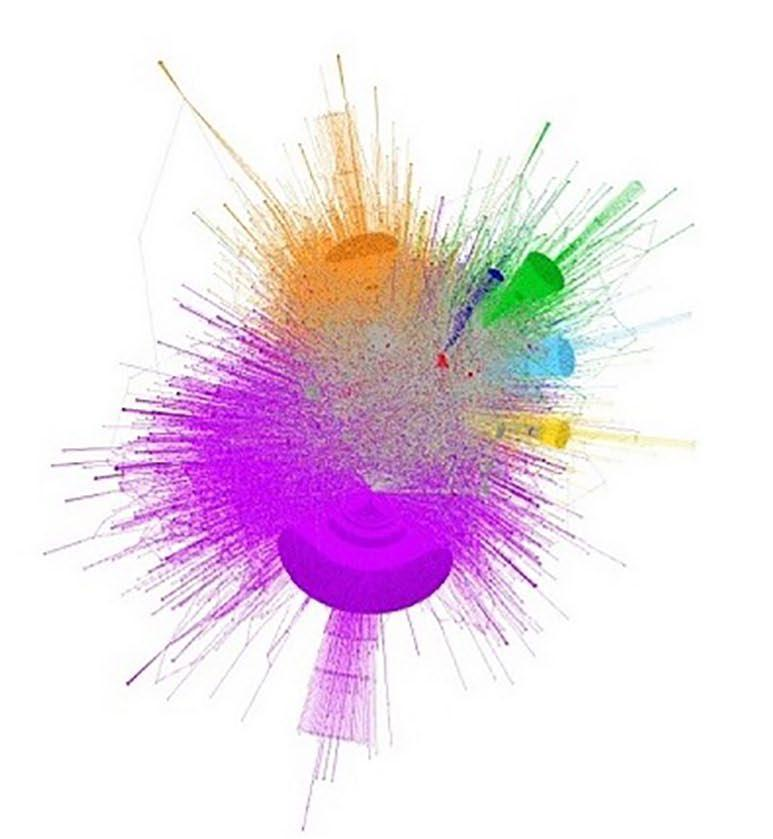
\includegraphics[width=0.5\linewidth]{discussionWebGraph1}}
		\hfill
		\subcaptionbox{\label{fig:discussionWebGraph-2}}{%
			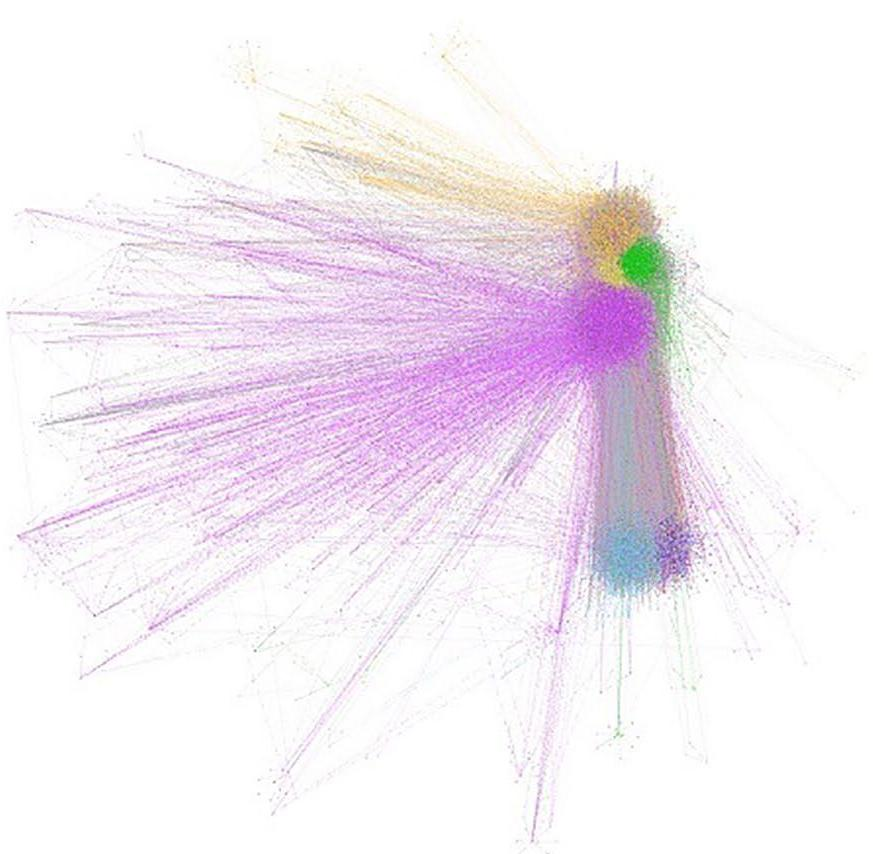
\includegraphics[width=0.5\linewidth]{discussionWebGraph2}}
		\hfill
	}
	\legend{lilac: commenters to \textit{Nexta};
		gray: users who commented in 2 to 5 accounts; 
		orange: commenters to \textit{Belsat};
		green: commenters to \textit{No guarantee};
		light blue: commenters to \textit{Popular reporter}; 
		yellow: commenters to \textit{Leave the Vagon!};
		blue: commenters to \textit{Rudabelka show-off};
		red: users who commented in all accounts.}
	\caption[Этот текст попадает в названия рисунков в списке рисунков]{The discussion web graph: (a) by the ForceAtlas2 algorithm and (б) by the OpenOrd algorithm}\label{fig:discussionWebGraph}
\end{figure}

As Figure~\cref{fig:discussionWebGraph} shows, attractiveness of the channels was unequal. Six of 10 commenters commented to \textit{Nexta}, and \textit{Nexta} only (59.34\%). \textit{Belsat} (11.54\%) and \textit{No guarantee} (5.35\%) came next, while \textit{Popular reporter} (3.62\%), \textit{Leave the Vagon!} (2.14\%), and \textit{Rudabelka show-off} (0.86\%) were least popular. This is explainable, given the latter channels’ local status.

Beside these users, circa 17\% of commenters united the channels and formed an inter-channel discussion core, as they commented to more than one channel. Thus, 7,076 users (16.96\%) commented on two to five channels; 75 users commented on all the six channels. The latter sub-sample will be used in our studies of the nature of Belarusian oppositional public.

To further clarify the core/periphery constellation, we have reconstructed the graph by another algorithm, OpenOrd (Figure~\cref{fig:discussionWebGraph-2}). Figure~\cref{fig:crossCommentersMetricsCurves} shows two modules, one comprising four channels and one with the two remaining ones, with gray and red users in between bridging densely the two nebulae. The periphery links mostly to Nexta and Belsat, the two channels closest to classic media by format. Activist chan- nels create denser commenting publics, but they are all interlinked.

\begin{figure}[ht]
	\centerfloat{
		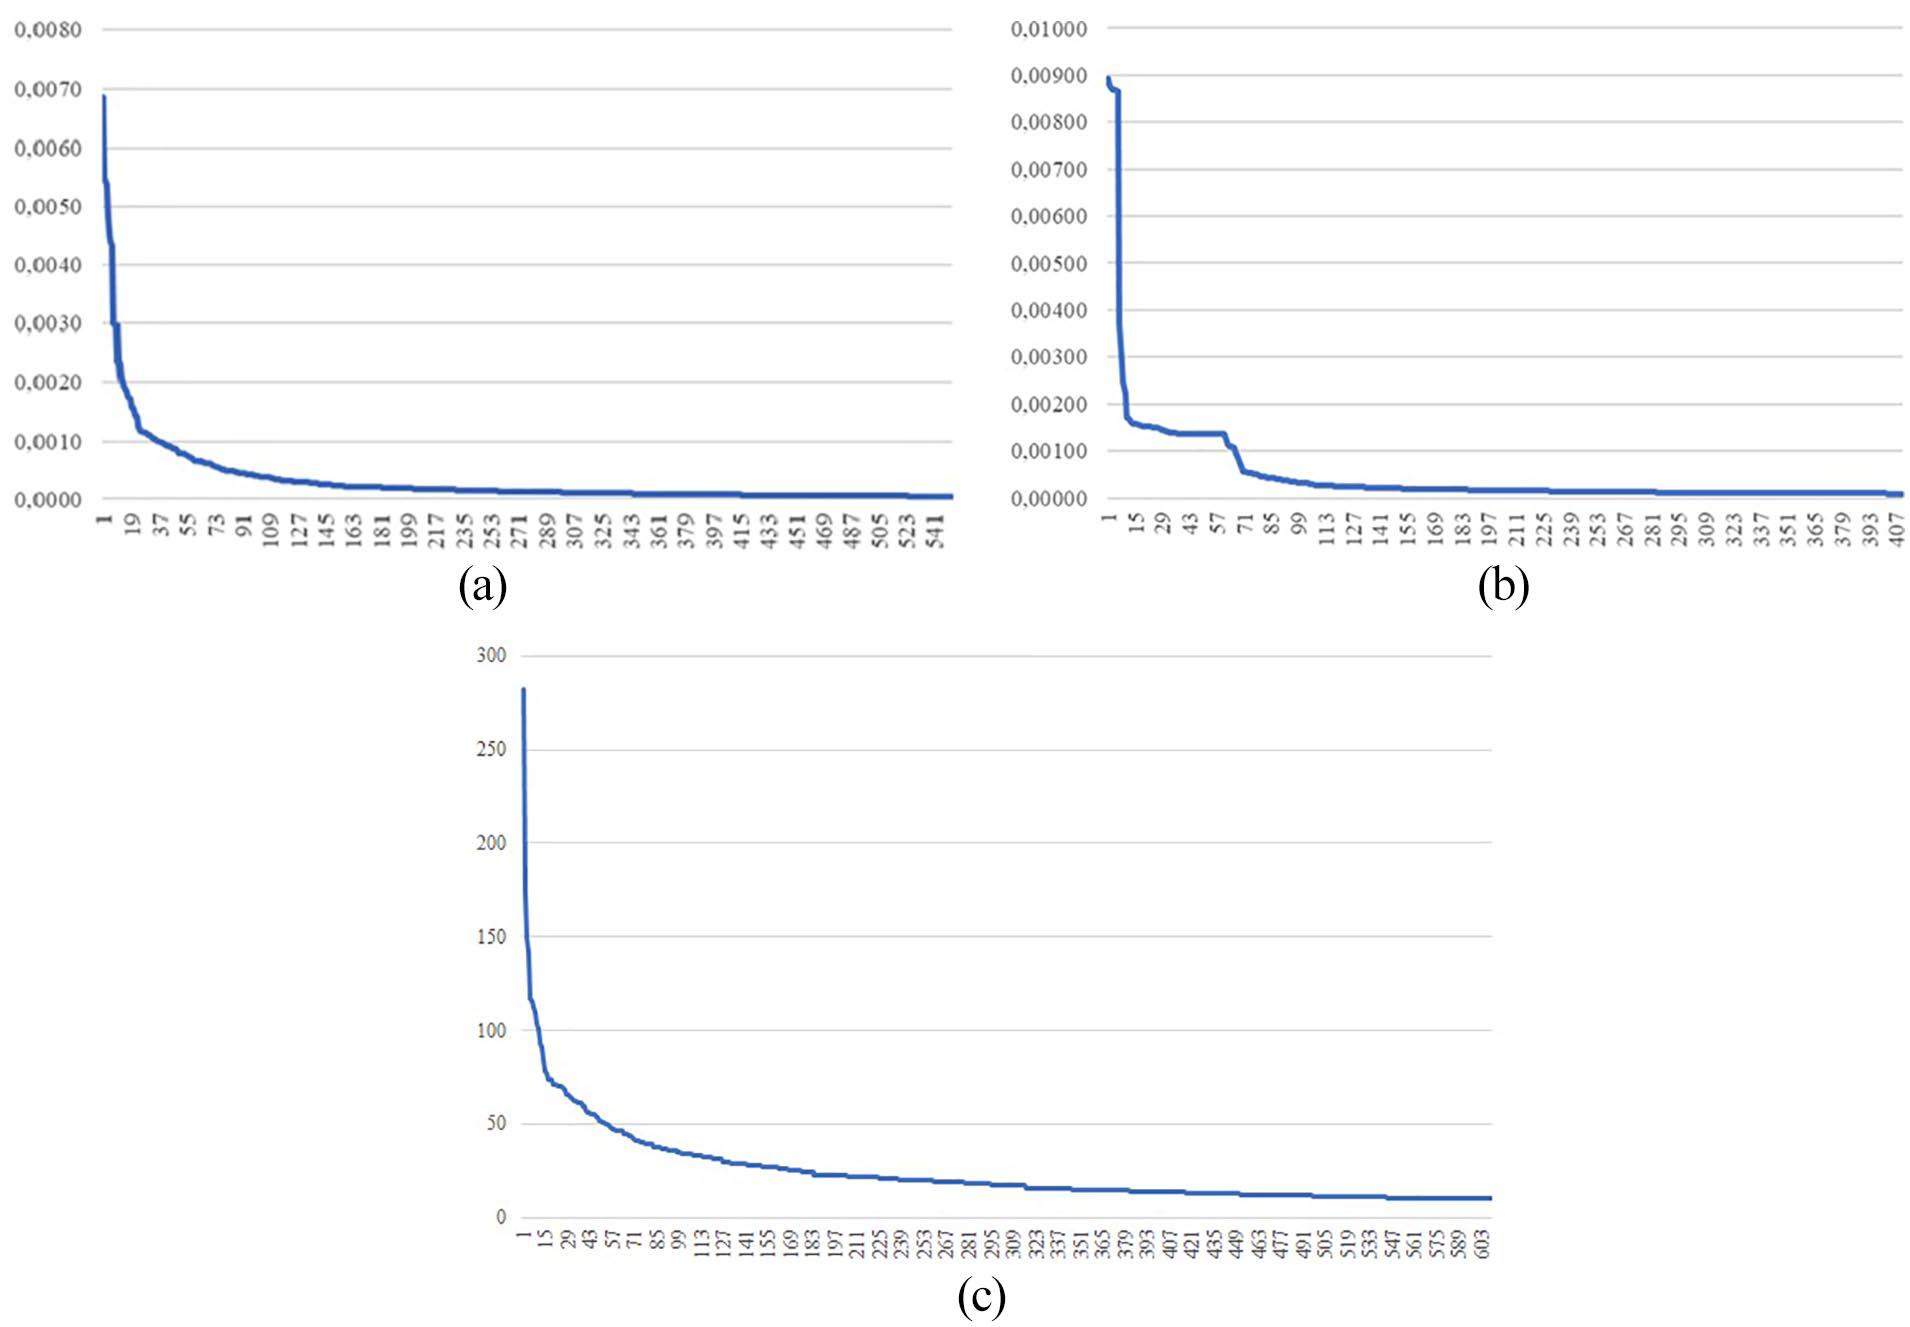
\includegraphics[scale=0.75]{crossCommentersMetricsCurves}
	}
	\caption{Cross-commenters’ metrics curves: (a) betweenness centrality (\(K\)), user long tail cut at user \#553 (\(K = 0.0001\)); (b) pagerank centrality (\(M\)), user long tail cut at user \#410 (\(M = 0.00001\)); (c) indegree centrality (\(N\)), user long tail cut at user \#610 (\(N = 10\)). The six commented accounts are excluded.}\label{fig:crossCommentersMetricsCurves}
\end{figure}

To avoid algorithms-induced distortions in our judgment, we have also assessed the curves of user graph metrics, namely betweenness, pagerank, and degree centralities (Figure~\cref{fig:crossCommentersMetricsCurves}). Graphs of betweenness (“user-as-crossroads” importance) and indegree (number of incoming comments) centralities show smooth decline, which means that the borders of the core are not sharp. The pagerank graph shows five important users (all being ordi- nary citizens) and a group of \(\sim 70\) users of secondary importance. Overall, the graphs reveal that the commenters were not a closed-up community the way that Belarusian authorities often depicted them but a public with a cross-commenting core and a wide but active periphery (3+ comments per user on average).

Also, we have assessed the top 100 users by the three centralities, to see whether they represented foreign institutions or citizens whose presence would support the claim of “foreign agents” used by the authorities to discredit the opposition. To our best possible judgment, within the three top 100 lists, there were several media-like channels (\textit{Belarusian world, Real Belarus! Homel Society}, and \textit{Selvestor Vivat} of oppositional stance, \textit{West Polesian} focusing on folk culture, \textit{fanzone fanzone} on sports, and \textit{RadioDestroyer} on self-made radio stations) and three foreign users (one male from Poland, one mum with a little daughter from Germany, one unidenti- fied). One alleged “foreign-agent-like” account, \textit{Biełarus z-za miažy} (Polish “Belarus from abroad”), indeed, was present within top 100 pagerank pages, but we could not learn its stance, as it was completely unavailable in 2021. One Polish account was also found among 76 cross-commenters.

Thus, the active public we have discovered was genuinely Belarusian, with only minor presence of foreign users and media-like initiatives.

\paragraph{RQ2: The Conflictual Nature of the Public}
Our coding of 8,644 posts shows that antagonism was highly salient (3,131 posts or 36.2\%); thus, the discourse was, indeed, permeated by conflict. However, agonistic/adversarial mood was also salient enough (1,112 posts or \(\sim13\)\%); but it manifested only in readiness to discuss (posing questions and reacting to statements in a responsive mode or partial agreement), not in readiness to recognize differences. Consensual claims beyond emotional support (198 posts or 2.9\%) related exclusively to agreement with co-thinkers and authors of the videos, not to agreeing with ideological counterparts.

Two other dimensions of agonism/antagonism were pres- ence of dialogue markers (2,087 posts or 24.1\%) and aggression (883 posts or 10.2\%). The share of aggressive posts resembles that on the Russian political YouTube \cite{BodrunovaLitvinenkoBlekanov2021}. Interestingly, correlations (see Table~\cref{tab:discursiveFeaturesCorrelationsComment}) show that dialogue is linked to both antagonism and agonism. For antagonism, this is due to aggressive rebuttals toward alleged pro-Russian trolls; and this explains why dialogue is also linked to aggression. For agonism, it is genuine dialogue with questions to fellow commenters. Expectedly, for individual comments, aggression directly correlated with antag- onism and inversely with agonism, thus proving that posing substantial questions lowers aggression (even slightly more than agreement does!).

\begin{table}[ht]%
	\centering
	\caption{Correlations of discursive features: on the level of a comment}%
	\label{tab:discursiveFeaturesCorrelationsComment}% label всегда желательно идти после caption
	\begin{adjustbox}{width=1\textwidth}
		\small
		\begin{tabular}{ l  l  l  l  l  l  l  l  l }% Вертикальные полосы не используются принципиально, как и лишние горизонтальные (допускается по ГОСТ 2.105 пункт 4.4.5) % @{} позволяет прижиматься к краям
			\toprule
			& Aggression & Criticism & \makecell[l]{Criticism:\\Leadership} & \makecell[l]{Criticism:\\Policy} & \makecell[l]{Criticism:\\Self} & Antagonism &  Agonism & Agreement \\
			\hline
			Dialogue & .\textbf{242**} & \textbf{\(-.213\)**} & \textbf{\(-.166\)**} & \(-.073\)** & \(-.056\)** & .143** & \textbf{.190**} & \\
			Aggression & 1 & \(-.044\)** & \textbf{.049**} & \textbf{\(-.080\)**} & \(-.084\)** & \textbf{.394**} & \textbf{\(-.099\)**} & \(-.049\)**\\
			Criticism &  & 1 & \textbf{.707**} & \textbf{.329**} & \textbf{.372**} & \textbf{.247**} & \(-.055\)** & \(-.070\)**\\
			Criticism: Leadership & & & 1 & \(-.102\)** & \textbf{\(-.146\)**} & \textbf{.361**} & \textbf{\(-.086\)**} & \(-.065\)**\\
			Criticism: Policy & & & & 1 & \(-.087\)** & \(-.061\)** & & \(-.024\)**\\
			Criticism: Self & & & & & 1 & \(-.071\)** & .033** & \\
			Antagonism & & & & & & 1 & \textbf{\(-.289\)**} & \textbf{\(-.112\)**}\\
			Agonism & & & & & & & 1 & \(-.059\)**\\
			Agreement & & & & & & & & 1\\
			\bottomrule
			\multicolumn{9}{@{}p{\textwidth}}{%
				%				\vspace*{-4ex}% этим подтягиваем повыше
				\hspace*{2.5em}% абзацный отступ - требование ГОСТ 2.105
				Note. *\(p \le .05\); **\(p \le .01\). Correlations supported on the aggregate level are in bold.
			}\\
		\end{tabular}%
	\end{adjustbox}
\end{table}

To check whether discursive features depended on the number of comments by one user, we aggregated the comments by user, calculated percentages of comments for each feature, and checked the dependencies (see Table~\cref{tab:discursiveFeaturesCorrelationsAggregate}). The main correlations were supported and only involvement into dialogue grew substantially when the number of comments by a user grew.

\begin{table}[ht]%
	\centering
	\caption{Correlations of discursive features: on the aggregate level}%
	\label{tab:discursiveFeaturesCorrelationsAggregate}% label всегда желательно идти после caption
	\begin{adjustbox}{width=1\textwidth}
		\small
		\begin{tabular}{ l  l  l  l  l  l  l  l  l  l  l }% Вертикальные полосы не используются принципиально, как и лишние горизонтальные (допускается по ГОСТ 2.105 пункт 4.4.5) % @{} позволяет прижиматься к краям
			\toprule
			& Dialogue & Aggression & Criticism & \makecell[l]{Criticism:\\Leadership} & \makecell[l]{Criticism:\\Policy} & \makecell[l]{Criticism:\\Self} & Antagonism &  Agonism & Agreement & \makecell[l]{Agonism +\\Agreement} \\
			\hline
			Number of comments & .416** & & &  & & & & & & \\
			
			Dialogue & 1 & .\textbf{299**} & \textbf{\(-.238\)**} & \textbf{\(-.249\)**} & & & & \textbf{.479**} & & .442**\\
			
			Aggression & & 1 & & \textbf{.425**} & \textbf{\(-.304\)**} & & \textbf{.790**} & \textbf{\(-.298\)**} &  & \(-.323\)**\\
			
			Criticism & & & 1 & \textbf{.766**} & \textbf{.305**} & \textbf{.327**} & \textbf{.511**} & & & \(-.055\)** \\
			
			Criticism: Leadership & & & & 1 & \(-.102\)** & & \textbf{\(-.268\)**} & \textbf{.629**} & \textbf{\(-.311\)**} & \(-.339\)**\\
			
			Criticism: Policy & & & & & 1 & \(-.087\)** & & & \(.229\)** & \\
			
			Criticism: Self & & & & & & 1 & & & & \\
			
			Antagonism & & & & & & & 1 & \textbf{\(-.340\)**} & \textbf{\(-.225\)**} & \(-.378**\)\\
			Agonism & & & & & & & & 1 & & \(.966\)**\\
			Agreement & & & & & & & & & 1& .439**\\
			\makecell[l]{Agonism +\\Agreement} & & & & & & & & & & 1\\
			\bottomrule
			\multicolumn{11}{@{}p{\textwidth}}{%
				%				\vspace*{-4ex}% этим подтягиваем повыше
				\hspace*{2.5em}% абзацный отступ - требование ГОСТ 2.105
				Note. *\(p \le .05\); **\(p \le .01\). Correlations supported on the aggregate level are in bold.
			}\\
		\end{tabular}%
	\end{adjustbox}
\end{table}

Median percentage for dialogical comments per author was less than 10\% (9.6\%), even if 25 of 75 users had \(\ge 20\%\) of dialogue-oriented comments. Aggression was much lower (median \(= 4.5\%\)), with 10 users posting \(\ge 20\%\) aggressive comments. However, antagonism was high (median \(= 33.4\%\)), with 64 users allowing it in \(\ge 20\%\) comments and 13 reaching \(\ge 50\%\), only partly compensated by agonism and agreement (combined median \(= 11.9\%\)).

Altogether, the shape of conflict on Belarusian oppositional YouTube was antagonistic, with commenters’ firm conviction of particular views, not seeking agreement with opponents, and dialogue mostly aiming at rebuttals toward alleged trolls. However, it was relatively non-aggressive and, in many cases, showed readiness to pose questions to opponents and co-thinkers.

\paragraph{RQ3: Direction of Criticism and Discursive Clusters}
However, the true main feature of the discourse was criticism. It differed from aggression (“The Ministry of Education and the education departments [of local administrations] are destroying our Belarusianness”), and was not always antagonistic.

Following Toepfl’s \cite{Toepfl} division of authoritarian publics into uncritical, policy-critical, and leadership-critical, we have coded presence of criticism and its direction. After preliminary reading, however, we have added one more category, which was self-criticism -- critique addressed to “us ourselves,” Belarus as a country/society, or oneself personally. Strikingly salient in the dataset, self-criticism sharply distinguished the Belarusian discourse from, for example, the Russian one of 2019. For the reasons of objectivity, we have also coded support to authorities as a counterbalance.

The latter, though, was expectedly next-to-absent, found in 17 comments, with 3 among 494 comments by one user as a maximum. Criticism, on the contrary, was present in 3,801 comments (\(\sim 44\%\)), with only one user having \(\le 20\%\) of critical posts, and 36 users of 75 being overwhelmingly critical (\(\ge 50\%\) comments). However, the direction/addressee of this criticism varied.

The highest amount of criticism was evoked by the “system” \cite{Ledeneva}, with the median \(= 27.7\%\). This included Aliaksandr Lukashenka himself; authorities in general and civil servants in particular; militiamen; and pro-Russian trolls. Lukashenka is described as “tsar” and \textit{peresident} (“over-sitter”), \textit{ne Bat’ka} (as “parents are not elected”), \textit{lukashescu} (reminiscent to Ceausescu), and \textit{lukavy} (“cunning”) afraid of his own people. More troubling, though, are rare descriptions of lukanomics and demands for dismantling of presidency as an institution, along with support of fair elections and freedoms:

\begin{displayquote}
	…Turnover of power, or, better, absence of presidentship in Belarus is key to normal statehood.
\end{displayquote}

The authorities are described as arrogant, shame-evoking, thieves who “feed themselves at the trough” while lying and imitating work, oppositional to people, and powerless to decide. Militiamen are compared to jackals and Hitlerjugend. Often, together they are compared to occupants, and the country is called “occupied” and people “enslaved.” Antagonism in the dataset was mostly linked to descriptions of power as insane, incompetent, barbaric, showing-off, mistrusted, unduly rich, incapable of negotiation, and laughable at. The hopeless mood of “the further the worse” was dominant.

Many comments are addressed to alleged pro-Russian commenters, while, in the core, there was only one pro-Russian user. Pro-Russians were shamed (sometimes aggressively) as trolls and bots, while recognizable responses to (pro-)European or (pro-)American commenters were extremely rare (six of all). This might be a sign of pro-Russian “trollization” of the periphery of the discussion, oppo- site to the authorities’ claims of European impact upon online communication. In contrast to trolls, oppositional bloggers are a “punch in the gut” to the “system.”

In Toepfl’s theory, leadership-critical publics, presumably, appear where policy-critical publics already exist. However, we have discovered a leadership-critical public without policy criticism. For a Western observer, this is a paradox; for autocratic publics, though, cursing “the system” without assessing its individual shortcomings is characteris- tic, due to absence of traditions of publicly discussing policies. For policy criticism, the median \(= 5\%\); the users only mentioned some examples of bad policy decisions, without giving reasons or suggesting alternatives.

Self-criticism was more impressive. It stably spread through the dataset, with the median \(= 9\%\), and included sarcasm toward official slogans like “Belarus -- a country for living,” criticizing \textit{pamyarkounasc}’ - forbearance and long-suffering viewed as traditional for Belarusians, and, most often, stating citizen’s responsibility for letting the country into its current state:

\begin{displayquote}
	Quite livable here -- for an American pensioner.
\end{displayquote}

\begin{displayquote}
	[I feel] shame, because we are all responsible that our country is ruled by exactly this [person].
\end{displayquote}

\begin{displayquote}
	Everyone wants change but no one wants to do anything.
\end{displayquote}

\begin{displayquote}
	We need, in general, an alternative Belarusian national life.
\end{displayquote}

The narrative of self-victimization intertwined with two more narratives -- the necessity of unified efforts and deeds instead of words within legal boundaries -- 

\begin{displayquote}
	I agree this is scary, but law needs to be our weapon, if we do not follow the law, we will become them.
\end{displayquote}

\begin{displayquote}
	Alas, most probably, no way via the courts, as this is their arms against ordinary people. <…> our only armament against the system is solidarity.
\end{displayquote}

\begin{displayquote}
	We need to find other ways. It will anyway depend fully on people’s activity.
\end{displayquote}

\begin{displayquote}
	Even a critical mass of amoebae will never explode.
\end{displayquote}

-- and the narrative of the aforementioned “third way” for Belarusians:

\begin{displayquote}
	We will go another way. Not to NATO, not to the Russian Federation. How about this option? Neutralism.
\end{displayquote}

The users state that they want to “make friends, not enemies” with “all the countries of the civilized world,” including Europe, the United States, and Russia -- which, regretfully for the commenters, choses more and more a way to self-isolation. In such statements, neither policy criticism nor self-criticism is linked to aggression (see Table~\cref{tab:discursiveFeaturesCorrelationsAggregate}), and the more leadership criticism is present, the less self-criticism is expressed by the users.

Another addition to Toepfl’s view is that discursive features like dialogue or aggression/antagonism need to be used in combination with criticism to define the types of autocratic publics. By using k-means clustering, we have shown that these features allow for seeing difference between actively aggressive-critical, passive-critical, non-aggressive dialogical modes of discussion (see Figure~\cref{label}).

\begin{figure}[ht]
	\centerfloat{
		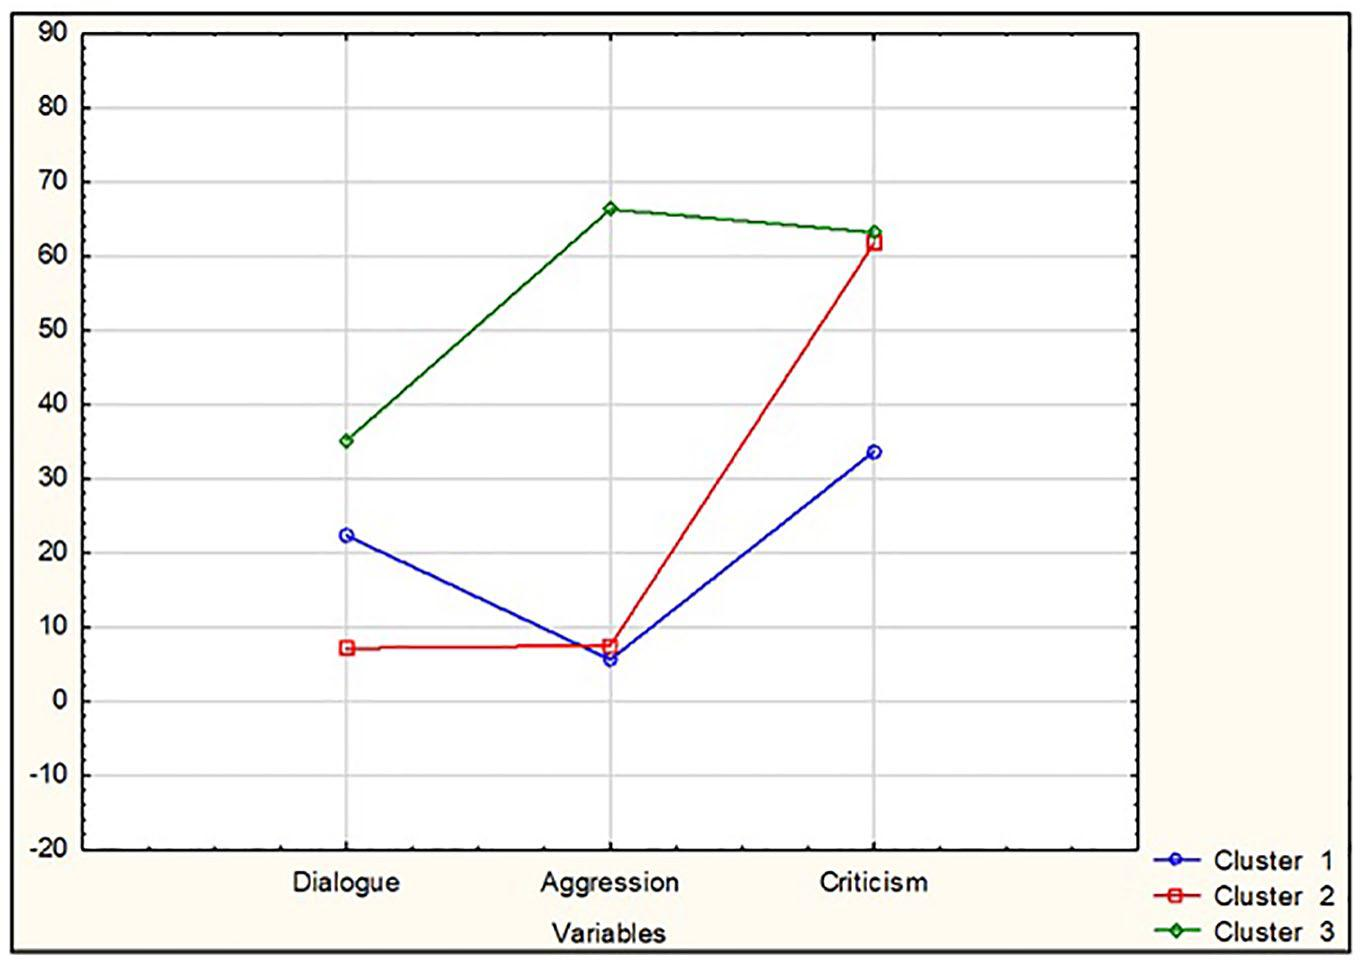
\includegraphics[scale=0.75]{crossCommentersSubClusters}
	}
	\caption{Sub-clusters of cross-commenters by discursive features. Three clusters represent the best decision by the silhouette metric; \(p \le .0000\) for all the clusters}\label{fig:crossCommentersSubClusters}
\end{figure}

\subsubsection{Discussion and Conclusion}

In general, what we have seen on Belarusian oppositional YouTube of 2018 was, to our viewpoint, the graduate cumulation of opinion that, in August 2020, reached a threshold and spilled over to Belarusian streets.

We have shown that, at least for 2018, the oppositional public on Belarusian YouTube was open but non-random; genuine but already highly alert against trolls and bots; detached from political parties but reaching the critical point of politicization. It bore the markers of readiness to massive protest, such as acknowledgment of people’s own guilt and calls for solidarity against the “system.” Without much dialogue on policing, criticism toward the systemic features of the state combined with unusually high self-blaming and non-acceptance of Belarus and Belarusians themselves in their long-suffering. The commenters’ positions reflected what later formed a countrywide consensus and partly laid a foundation for the 2020 protests.

Studies like ours allow for capturing the public mood better than polls or political party research; we have detected a combination of readiness for change, “adversarial antagonism,” and self-criticism. The Belarusian case demonstrates that antagonism on social media is a double-edged sword: it allows uniting in hatred but eliminates chances for deliberation of participants with opposing standpoints.

Our additions to the theory of autocratic publics include presence of leadership-critical publics without policy criticism in their discourse, lack of policy-and-leadership criticism, importance of self-critical narratives, and multi-dimensionality of discourses and (if publics are characterized by discourses) of publics. The linkages between antagonism/agonism and criticism of various directions need to be further explored, too. And, last but not the least, tracing today’s changes in the Belarusian oppositional discourse online would provide a unique chance to see how such discourses mutate after a relative failure (or victory?) of a nationwide resistance wave.

\FloatBarrier
